\documentclass[a4paper,twoside,10pt,openright]{report}%Dokumentenklasse 
\usepackage{graphicx} %Compiler

\usepackage{dsfont}

%%%% Schrift und Kodierung %%%%
	\usepackage[T1]{fontenc} %Zeichensatzkodierung von 7bit auf 8bit 
	\usepackage[utf8]{inputenc} %Zeichensatzkodierung Unicode bzw. UTF8
	\usepackage{lmodern} %Vektorschrift
	%\RequirePackage[english,spanish,es-nolayout]{babel}
	\usepackage[english]{babel}
	\usepackage{textcomp}
	\usepackage{lmodern}
	\usepackage{url}
	\usepackage[bookmarksnumbered=true]{hyperref}
    \graphicspath{{figures/}}	
	
%%% COLORS %%%
\newcommand{\hl}[1]{
   \textcolor{MidnightBlue!90!black}{#1} 
}

\usepackage{pifont}% http://ctan.org/pkg/pifont
\newcommand{\cmark}{\ding{51}}%
\newcommand{\xmark}{\ding{55}}%

\usepackage{stackrel}

\usepackage{feynmp}

\usepackage{amsthm}
\newtheorem{definition}{Definition}
\newtheorem{proposition}{Proposition}
	
%%%% Fancy Header %%%
\usepackage{fancyhdr}
\usepackage[dvipsnames]{xcolor}
\usepackage{tikz} 
\usepackage{pgfplots}
%\usepackage{pgf-pie}

\usetikzlibrary{arrows}
\usetikzlibrary{shapes.geometric, arrows}

\definecolor{mycolor}{rgb}{0.45,0.45,0.45}% dark grey

\newcommand{\mcD}{\mathcal{D}}
\newcommand{\mcL}{\mathcal{L}}
\newcommand{\dth}{\Delta_{\text{th/sys}}}
\newcommand{\dst}{\Delta_{\text{stat}}}
\newcommand{\dsy}{\Delta_{\text{syst}}}
\newcommand{\sthsy}{\sigma_{\text{th/sys}}}
\newcommand{\sth}{\sigma_{\text{th}}}
\newcommand{\sst}{\sigma_{\text{stat}}}
\newcommand{\ssy}{\sigma_{\text{syst}}}

\newcommand{\Langle}{\big\langle}
\newcommand{\Rangle}{\big\rangle} 
 
\fancyhf{}
\fancyhead[LE]{\sffamily\color{mycolor}\nouppercase{\leftmark}} % left even, right odd
\fancyhead[RO]{\sffamily\color{mycolor}\nouppercase{\rightmark}} % left even, right odd
\fancyfoot[CE,CO]{\sffamily\color{mycolor}\nouppercase{\thepage}} % center even, center odd
\renewcommand{\headrule}{{\color{mycolor}%
\hrule width\headwidth height\headrulewidth \vskip-\headrulewidth}}
\renewcommand{\headrulewidth}{0.5pt}

\fancypagestyle{plain}{%
    \fancyhf{}%
    \fancyfoot[CE,CO]{ { \sffamily\color{mycolor}{\thepage} } }
	\renewcommand{\headrulewidth}{0.0pt}
}

%\fancypagestyle{fancy}{%
%   \fancyhf{}
%	\fancyhead[LE,RO]{\sffamily\color{mycolor}\nouppercase{\leftmark}} % left even, right odd
%	\fancyfoot[CE,CO]{\sffamily\color{mycolor}\nouppercase{\thepage}} % center even, center odd
%	\renewcommand{\headrule}{{\color{mycolor}%
%	\hrule width\headwidth height\headrulewidth \vskip-\headrulewidth}}
%	\renewcommand{\headrulewidth}{0.5pt}
%}


%%% Customize titles %%%%
\usepackage[ ]{titlesec}  %
\usepackage{etoolbox}
\makeatletter
\patchcmd{\ttlh@hang}{\parindent\z@}{\parindent\z@\leavevmode}{}{}
\patchcmd{\ttlh@hang}{\noindent}{}{}{}
\makeatother
%\titleformat{\chapter}[display]
%  { \normalsize \huge  \color{black}}%
%  {\flushright \normalsize \color{mycolor} \MakeUppercase %
%  {\sffamily \chaptertitlename } \hspace{1 ex}%
%  { \fontsize{60}{60}\selectfont \color{mycolor} \sffamily  \thechapter }}%
%  {10 pt}%
%  {\sffamily \huge \color{mycolor}\bfseries}
%\newcommand\mychapformat[1]{\parbox[t]{\dimexpr\textwidth-3em\relax}{\raggedleft#1}}
\titleformat{\chapter}[hang]{\Huge\bfseries\color{mycolor}\sffamily}% the number
	{\thechapter\hspace{20pt}\textcolor{mycolor}{|}\hspace{20pt}}%
	{0pt}{\Huge\bfseries\color{mycolor}\sffamily}% the title
\titleformat*{\section}{\sffamily\LARGE\color{mycolor}}
\titleformat*{\subsection}{\sffamily\Large\color{mycolor}}
\titleformat*{\subsubsection}{\sffamily\large\color{mycolor}}
\titleformat*{\paragraph}{\sffamily\large\bfseries\color{mycolor}}



	
%%%% Mathepakete %%%%
	\usepackage{array}
	\usepackage{calc}
	\usepackage{amsmath}
	\usepackage[intlimits]{empheq}
	\usepackage{amssymb,mathrsfs}
	\usepackage{theorem}
	\usepackage{slashed}
	\usepackage{feynmp-auto}

%%%% Sonstiges %%%%
	%\usepackage{subcaption}
	\expandafter\def\csname ver@subfig.sty\endcsname{}
	\usepackage{subfig} %Ermöglicht subfloats, also mehrere Tabellen/Bilder in einer Umgebung
	\usepackage{float} %Setzt mit [H] Figuren genau dort hin, wo sie im Text auftauchen
	\usepackage{booktabs} %Andere Tabellen
	\usepackage{gensymb}
	\usepackage{extarrows}%lange Pfeile
%	\usepackage{pst-pdf}	
	\usepackage{wasysym} %Symbolpaket
	\usepackage{multirow} %Ein Wert für mehrere Zeilen oder Spalten von Tabellen. Verwendung \multirow{#AnzahlZeilen}{*}{Name} bzw. analog \multicolumn{}{}{}
	\usepackage{rotating} %ermöglicht Schiefe Schrift
	%\usepackage{ziffer} %Deutsche Zahlen (Komma als Dezimalstelle im Mathemodus!)
	\usepackage{nicefrac} %Im Text schöne Brüche
	\usepackage[inner=3cm, outer=2.4cm, top=3cm]{geometry} %Passt Seitenränder an (left, right, top, bottom, width, height, textwidth, textheight)
	\usepackage{scrhack} %Verbessert angeblich LaTeX-Pakete
	\usepackage{numprint} %ROOT-Zahlen in deutsches zahlenformat übertragen. Syntax: \numprint[kg]{1.234e56} wird zu 1,234 * 10^56 kg
	\usepackage{cite}
	\usepackage{placeins}
	\usepackage{changepage}
	%\hyphenation{con-fine-ment}
	
%%%% spezielle Formatierungen %%%%
	\setlength{\emergencystretch}{25pt} %verhindert das Herausragen von Wörtern übers Zeilenende
	\setlength{\parindent}{0pt} %Kein Einschub bei neuem Absatz
	\setlength{\parskip}{2pt plus 1pt} %Erhöht Abstand zwischen Absätzen (um 1pt flexibel bei Seitenumbrüchen)
	
	%%%% Dokument-Variablen %%%%
\date{\today}

%%%% Eigene Befehle %%%%
\DeclareGraphicsRule{*}{mps}{*}{}
	\newcommand{\mE}[1]{\,\mathrm{#1}} %Einheiten im Mathemodus
	\renewcommand{\sl}[1]{\slashed{#1}} %Feynman-Slash
	\newcommand{\dummyImage}[2]{  %Erzeugt eine Umgebung wie includegraphics
		\frame{\mbox{\rule{0pt}{#2}	Bild fehlt  noch \rule{#1}{0pt}}}
	}
	\renewcommand{\i}{\mathrm{i}} %Imaginäre Einheit
%	\renewcommand{\vec}[1]{\textbf{#1}} %Fette Vektoren
	\newcommand{\bc}{\begin{center}}
	\newcommand{\ec}{\end{center}}

\newcommand{\matM}{\mathcal{M}}
\newcommand{\matH}{\mathcal{H}}
\newcommand{\matS}{\mathcal{S}}
\newcommand{\matU}{\mathcal{U}}
\newcommand{\matUL}{\mathcal{U}_L}
\newcommand{\matUR}{\mathcal{U}_R}

%%% center all the figures and tables
\makeatletter
\g@addto@macro\@floatboxreset\centering
\makeatother

% maximal number of floating environments on each page 
\setlength{\floatsep}{0pt}
\setcounter{topnumber}{1}
\setcounter{bottomnumber}{1}
\setcounter{totalnumber}{1}
\renewcommand{\topfraction}{1.0}
\renewcommand{\bottomfraction}{1.0}
\renewcommand{\textfraction}{0.0}
\renewcommand{\thefootnote}{\fnsymbol{footnote}}

\def\tablename{Table}
\def\figurename{Figure}

\newcommand{\newparagraph}{\par\bigskip\noindent}
\newcommand{\toolfont}[1]{\texttt{#1}}
\newcommand{\ord}{\ensuremath{\mathcal{O}}}
\newcommand{\ope}[1]{\ensuremath{\mathcal{O}_{#1}}}
\newcommand{\largex}{\ensuremath{\large \boldsymbol{\times}}}
\newcommand{\brlargex}{\ensuremath{\large (\boldsymbol{\times})}}
\newcommand{\mheavy}{\ensuremath{M}}

\newcommand{\lag}{\ensuremath{\mathcal{L}}}
\newcommand{\mat}{\ensuremath{\mathcal{M}}}
\newcommand{\delx}{\ensuremath{\Delta}}
\newcommand{\data}{\ensuremath{\mathcal{D}}}
\newcommand{\jump}{\vspace{0.3cm}}
\newcommand{\bsg}{\ensuremath{\mathcal{B}(b \to s \gamma)}}
\newcommand{\rself}{\ensuremath{\hat{\Sigma}}}
\newcommand{\retildehat}{\ensuremath{\mbox{Re}\hat{\Sigma}}}
\newcommand{\retilde}{\ensuremath{\mbox{Re}\,\Sigma}}
\newcommand{\dweaksing}{\ensuremath{\delta_{\text{weak}}^{\text{sing}}}}
\newcommand{\dweak}{\ensuremath{\delta_{\text{weak}}}}
\newcommand{\newtext}[1]{\textcolor{red}{#1}}
\newcommand{\suit}{\textcolor{blue}{$\spadesuit$}}
\newcommand{\neutn}{\ensuremath{\tilde{\chi}^0_n}}
\newcommand{\gluino}{\ensuremath{\tilde{g}}}
\newcommand{\squark}{\ensuremath{\tilde{q}}}
\newcommand{\met}{\ensuremath{\slashed{E}_T}}
\newcommand{\nqsq}{\ensuremath{\tilde{\chi}\,\tilde{q}\,q}}
\newcommand{\msbar}{\ensuremath{\overline{MS}}}
\newcommand{\sw}{\ensuremath{s_w}}
\newcommand{\swd}{\ensuremath{s^2_w}}
\newcommand{\cw}{\ensuremath{c_w}}
\newcommand{\cwd}{\ensuremath{c^2_w}}
\newcommand{\myrbox}[1]{\parbox{4.0cm}{#1}}

\usepackage{xspace}
\newcommand{\brinv}{\ensuremath{BR_{\text{inv}}}\xspace}
\newcommand{\vegas}{\textsc{Vegas}\xspace}
\newcommand{\madgraph}{\textsc{Madgraph}\xspace}
\newcommand{\geant}{\textsc{Geant4}\xspace}
\newcommand{\pythia}{\textsc{Pythia}8\xspace}
\newcommand{\fastjet}{\textsc{FastJet}\xspace}
\newcommand{\delphes}{\textsc{Delphes}\xspace}
\newcommand{\sherpa}{\textsc{Sherpa}\xspace}
\newcommand{\sklearn}{\textsc{scikit-learn}\xspace}
\newcommand{\keras}{\textsc{Keras}\xspace}
\newcommand{\tensorflow}{\textsc{TensorFlow}\xspace}
\newcommand{\pytorch}{\textsc{PyTorch}\xspace}
\newcommand{\theano}{\textsc{Theano}\xspace}
\newcommand{\adam}{\textsc{Adam}\xspace}

\newcommand{\psib}{\overline{\psi}}
\newcommand{\bpm}{\begin{pmatrix}}
\newcommand{\epm}{\end{pmatrix}}

\newcommand{\p}{\partial}
\newcommand{\br}{\text{BR}}
\newcommand{\qqquad}{\qquad \qquad}
\newcommand{\qqqquad}{\qquad \qquad \qquad}

\newcommand{\matx}{|\mathcal{M}|^2}
\newcommand{\really}{\stackrel{!}{=}}
\newcommand{\SFitter}{\textsc{SFitter} }

% units of measure
\newcommand{\mev}{{\ensuremath\rm MeV}}
\newcommand{\gev}{{\ensuremath\rm GeV}}
\newcommand{\tev}{{\ensuremath\rm TeV}}
\newcommand{\fb}{{\ensuremath\rm fb}}
\newcommand{\ab}{{\ensuremath\rm ab}}
\newcommand{\pb}{{\ensuremath\rm pb}}
\newcommand{\sign}{{\ensuremath\rm sign}}
\newcommand{\iab}{\text{ab}^{-1}}
\newcommand{\ifb}{{\ensuremath\rm fb^{-1}}}
\newcommand{\ipb}{{\ensuremath\rm pb^{-1}}}

% really great macro by Chris Lester
\def\slashchar#1{\setbox0=\hbox{$#1$}           % set a box for #1
   \dimen0=\wd0                                 % and get its size
   \setbox1=\hbox{/} \dimen1=\wd1               % get size of /
   \ifdim\dimen0>\dimen1                        % #1 is bigger
      \rlap{\hbox to \dimen0{\hfil/\hfil}}      % so center / in box
      #1                                        % and print #1
   \else                                        % / is bigger
      \rlap{\hbox to \dimen1{\hfil$#1$\hfil}}   % so center #1
      /                                         % and print /
   \fi}
\newcommand{\dslash}{\slashchar{\partial}}
\newcommand{\Dslash}{\slashchar{D}}

\def\eg{{e.g.}\ }
\def\ie{{i.e.}\ }
%\def\etal{{\sl et al} \,}
%\DeclareMathOperator{\tr}{Tr}
\newcommand{\pbp}{\ensuremath{H^\dagger\,H}}
\DeclareMathOperator{\tr}{Tr}
\newcommand{\Dfb}{\mbox{$\raisebox{2mm}{\boldmath ${}^\leftrightarrow$}\hspace{-4mm} D$}}
\newcommand{\Dfba}{\mbox{$\raisebox{2mm}{\boldmath ${}^\leftrightarrow$}\hspace{-4mm} D^a$}}
\newcommand{\overbar}[1]{\mkern 1.5mu\overline{\mkern-1.5mu#1\mkern-1.5mu}\mkern 1.5mu}
\let\vec\mathbf % vectors in bold
\renewcommand{\d}{\text{d}}



\addto\captionsenglish{\renewcommand{\bibname}{References}}
%\bibliographystyle{utphys}
\pagestyle{fancy}

\begin{document}
\begin{fmffile}{feynman}
%\maketitle

\pagenumbering{alph}
\thispagestyle{empty}
\mbox{}
\vspace*{5mm}
\begin{center}
\sffamily
\large
Dissertation\\[1.5mm]
submitted to the\\[1.5mm] 
Combined Faculties of the Natural Sciences and Mathematics\\[1.5mm]
of the Ruperto-Carola-University of Heidelberg, Germany \\[1.5mm]
for the degree of \\[1.5mm]
Doctor of Natural Sciences


\vfill
{
\normalsize
Put forward by\\[1.5mm]
Marco Bellagente\\
born in Desio\\
Oral examination: XX.XX.2022
}
\end{center}
\clearpage{\pagestyle{empty}\cleardoublepage}

\newpage
\thispagestyle{empty}
\mbox{}
\vspace*{3cm}
\sffamily
\begin{center}
%\rule[.3ex]{11cm}{1pt}\\
\line(2,0){310}\\[3mm]
\Huge{Go with the Flow}\\[2mm]
\Large{Normalizing Flow applications for High Energy Physics}\\[3mm]
\line(1,0){310}
%\rule[.3ex]{11cm}{1pt}
\end{center}


\vfill
\begin{tabular}{ll}
Referees: &  Prof. Dr. Jan-Martin Pawlowski\\[2mm]
               &  Prof. Dr. Monica Dunford \\
\end{tabular}

\rmfamily

\newpage
%\pagestyle{plain}
\clearpage{\pagestyle{empty}\clearpage}

%\documentclass[a4paper,twoside,10pt,openright]{report}%Dokumentenklasse 
\usepackage{graphicx} %Compiler

\usepackage{dsfont}

%%%% Schrift und Kodierung %%%%
	\usepackage[T1]{fontenc} %Zeichensatzkodierung von 7bit auf 8bit 
	\usepackage[utf8]{inputenc} %Zeichensatzkodierung Unicode bzw. UTF8
	\usepackage{lmodern} %Vektorschrift
	%\RequirePackage[english,spanish,es-nolayout]{babel}
	\usepackage[english]{babel}
	\usepackage{textcomp}
	\usepackage{lmodern}
	\usepackage{url}
	\usepackage[bookmarksnumbered=true]{hyperref}
    \graphicspath{{figures/}}	
	
%%% COLORS %%%
\newcommand{\hl}[1]{
   \textcolor{MidnightBlue!90!black}{#1} 
}

\usepackage{pifont}% http://ctan.org/pkg/pifont
\newcommand{\cmark}{\ding{51}}%
\newcommand{\xmark}{\ding{55}}%

\usepackage{stackrel}

\usepackage{feynmp}

\usepackage{amsthm}
\newtheorem{definition}{Definition}
\newtheorem{proposition}{Proposition}
	
%%%% Fancy Header %%%
\usepackage{fancyhdr}
\usepackage[dvipsnames]{xcolor}
\usepackage{tikz} 
\usepackage{pgfplots}
%\usepackage{pgf-pie}

\usetikzlibrary{arrows}
\usetikzlibrary{shapes.geometric, arrows}

\definecolor{mycolor}{rgb}{0.45,0.45,0.45}% dark grey

\newcommand{\mcD}{\mathcal{D}}
\newcommand{\mcL}{\mathcal{L}}
\newcommand{\dth}{\Delta_{\text{th/sys}}}
\newcommand{\dst}{\Delta_{\text{stat}}}
\newcommand{\dsy}{\Delta_{\text{syst}}}
\newcommand{\sthsy}{\sigma_{\text{th/sys}}}
\newcommand{\sth}{\sigma_{\text{th}}}
\newcommand{\sst}{\sigma_{\text{stat}}}
\newcommand{\ssy}{\sigma_{\text{syst}}}

\newcommand{\Langle}{\big\langle}
\newcommand{\Rangle}{\big\rangle} 
 
\fancyhf{}
\fancyhead[LE]{\sffamily\color{mycolor}\nouppercase{\leftmark}} % left even, right odd
\fancyhead[RO]{\sffamily\color{mycolor}\nouppercase{\rightmark}} % left even, right odd
\fancyfoot[CE,CO]{\sffamily\color{mycolor}\nouppercase{\thepage}} % center even, center odd
\renewcommand{\headrule}{{\color{mycolor}%
\hrule width\headwidth height\headrulewidth \vskip-\headrulewidth}}
\renewcommand{\headrulewidth}{0.5pt}

\fancypagestyle{plain}{%
    \fancyhf{}%
    \fancyfoot[CE,CO]{ { \sffamily\color{mycolor}{\thepage} } }
	\renewcommand{\headrulewidth}{0.0pt}
}

%\fancypagestyle{fancy}{%
%   \fancyhf{}
%	\fancyhead[LE,RO]{\sffamily\color{mycolor}\nouppercase{\leftmark}} % left even, right odd
%	\fancyfoot[CE,CO]{\sffamily\color{mycolor}\nouppercase{\thepage}} % center even, center odd
%	\renewcommand{\headrule}{{\color{mycolor}%
%	\hrule width\headwidth height\headrulewidth \vskip-\headrulewidth}}
%	\renewcommand{\headrulewidth}{0.5pt}
%}


%%% Customize titles %%%%
\usepackage[ ]{titlesec}  %
\usepackage{etoolbox}
\makeatletter
\patchcmd{\ttlh@hang}{\parindent\z@}{\parindent\z@\leavevmode}{}{}
\patchcmd{\ttlh@hang}{\noindent}{}{}{}
\makeatother
%\titleformat{\chapter}[display]
%  { \normalsize \huge  \color{black}}%
%  {\flushright \normalsize \color{mycolor} \MakeUppercase %
%  {\sffamily \chaptertitlename } \hspace{1 ex}%
%  { \fontsize{60}{60}\selectfont \color{mycolor} \sffamily  \thechapter }}%
%  {10 pt}%
%  {\sffamily \huge \color{mycolor}\bfseries}
%\newcommand\mychapformat[1]{\parbox[t]{\dimexpr\textwidth-3em\relax}{\raggedleft#1}}
\titleformat{\chapter}[hang]{\Huge\bfseries\color{mycolor}\sffamily}% the number
	{\thechapter\hspace{20pt}\textcolor{mycolor}{|}\hspace{20pt}}%
	{0pt}{\Huge\bfseries\color{mycolor}\sffamily}% the title
\titleformat*{\section}{\sffamily\LARGE\color{mycolor}}
\titleformat*{\subsection}{\sffamily\Large\color{mycolor}}
\titleformat*{\subsubsection}{\sffamily\large\color{mycolor}}
\titleformat*{\paragraph}{\sffamily\large\bfseries\color{mycolor}}



	
%%%% Mathepakete %%%%
	\usepackage{array}
	\usepackage{calc}
	\usepackage{amsmath}
	\usepackage[intlimits]{empheq}
	\usepackage{amssymb,mathrsfs}
	\usepackage{theorem}
	\usepackage{slashed}
	\usepackage{feynmp-auto}

%%%% Sonstiges %%%%
	%\usepackage{subcaption}
	\expandafter\def\csname ver@subfig.sty\endcsname{}
	\usepackage{subfig} %Ermöglicht subfloats, also mehrere Tabellen/Bilder in einer Umgebung
	\usepackage{float} %Setzt mit [H] Figuren genau dort hin, wo sie im Text auftauchen
	\usepackage{booktabs} %Andere Tabellen
	\usepackage{gensymb}
	\usepackage{extarrows}%lange Pfeile
%	\usepackage{pst-pdf}	
	\usepackage{wasysym} %Symbolpaket
	\usepackage{multirow} %Ein Wert für mehrere Zeilen oder Spalten von Tabellen. Verwendung \multirow{#AnzahlZeilen}{*}{Name} bzw. analog \multicolumn{}{}{}
	\usepackage{rotating} %ermöglicht Schiefe Schrift
	%\usepackage{ziffer} %Deutsche Zahlen (Komma als Dezimalstelle im Mathemodus!)
	\usepackage{nicefrac} %Im Text schöne Brüche
	\usepackage[inner=3cm, outer=2.4cm, top=3cm]{geometry} %Passt Seitenränder an (left, right, top, bottom, width, height, textwidth, textheight)
	\usepackage{scrhack} %Verbessert angeblich LaTeX-Pakete
	\usepackage{numprint} %ROOT-Zahlen in deutsches zahlenformat übertragen. Syntax: \numprint[kg]{1.234e56} wird zu 1,234 * 10^56 kg
	\usepackage{cite}
	\usepackage{placeins}
	\usepackage{changepage}
	%\hyphenation{con-fine-ment}
	
%%%% spezielle Formatierungen %%%%
	\setlength{\emergencystretch}{25pt} %verhindert das Herausragen von Wörtern übers Zeilenende
	\setlength{\parindent}{0pt} %Kein Einschub bei neuem Absatz
	\setlength{\parskip}{2pt plus 1pt} %Erhöht Abstand zwischen Absätzen (um 1pt flexibel bei Seitenumbrüchen)
	
	%%%% Dokument-Variablen %%%%
\date{\today}

%%%% Eigene Befehle %%%%
\DeclareGraphicsRule{*}{mps}{*}{}
	\newcommand{\mE}[1]{\,\mathrm{#1}} %Einheiten im Mathemodus
	\renewcommand{\sl}[1]{\slashed{#1}} %Feynman-Slash
	\newcommand{\dummyImage}[2]{  %Erzeugt eine Umgebung wie includegraphics
		\frame{\mbox{\rule{0pt}{#2}	Bild fehlt  noch \rule{#1}{0pt}}}
	}
	\renewcommand{\i}{\mathrm{i}} %Imaginäre Einheit
%	\renewcommand{\vec}[1]{\textbf{#1}} %Fette Vektoren
	\newcommand{\bc}{\begin{center}}
	\newcommand{\ec}{\end{center}}

\newcommand{\matM}{\mathcal{M}}
\newcommand{\matH}{\mathcal{H}}
\newcommand{\matS}{\mathcal{S}}
\newcommand{\matU}{\mathcal{U}}
\newcommand{\matUL}{\mathcal{U}_L}
\newcommand{\matUR}{\mathcal{U}_R}

%%% center all the figures and tables
\makeatletter
\g@addto@macro\@floatboxreset\centering
\makeatother

%% maximal number of floating environments on each page 
\setlength{\floatsep}{0pt}
\setcounter{topnumber}{1}
\setcounter{bottomnumber}{1}
\setcounter{totalnumber}{1}
\renewcommand{\topfraction}{1.0}
\renewcommand{\bottomfraction}{1.0}
\renewcommand{\textfraction}{0.0}
\renewcommand{\thefootnote}{\fnsymbol{footnote}}

\def\tablename{Table}
\def\figurename{Figure}

\newcommand{\newparagraph}{\par\bigskip\noindent}
\newcommand{\toolfont}[1]{\texttt{#1}}
\newcommand{\ord}{\ensuremath{\mathcal{O}}}
\newcommand{\ope}[1]{\ensuremath{\mathcal{O}_{#1}}}
\newcommand{\largex}{\ensuremath{\large \boldsymbol{\times}}}
\newcommand{\brlargex}{\ensuremath{\large (\boldsymbol{\times})}}
\newcommand{\mheavy}{\ensuremath{M}}

\newcommand{\lag}{\ensuremath{\mathcal{L}}}
\newcommand{\mat}{\ensuremath{\mathcal{M}}}
\newcommand{\delx}{\ensuremath{\Delta}}
\newcommand{\data}{\ensuremath{\mathcal{D}}}
\newcommand{\jump}{\vspace{0.3cm}}
\newcommand{\bsg}{\ensuremath{\mathcal{B}(b \to s \gamma)}}
\newcommand{\rself}{\ensuremath{\hat{\Sigma}}}
\newcommand{\retildehat}{\ensuremath{\mbox{Re}\hat{\Sigma}}}
\newcommand{\retilde}{\ensuremath{\mbox{Re}\,\Sigma}}
\newcommand{\dweaksing}{\ensuremath{\delta_{\text{weak}}^{\text{sing}}}}
\newcommand{\dweak}{\ensuremath{\delta_{\text{weak}}}}
\newcommand{\newtext}[1]{\textcolor{red}{#1}}
\newcommand{\suit}{\textcolor{blue}{$\spadesuit$}}
\newcommand{\neutn}{\ensuremath{\tilde{\chi}^0_n}}
\newcommand{\gluino}{\ensuremath{\tilde{g}}}
\newcommand{\squark}{\ensuremath{\tilde{q}}}
\newcommand{\met}{\ensuremath{\slashed{E}_T}}
\newcommand{\nqsq}{\ensuremath{\tilde{\chi}\,\tilde{q}\,q}}
\newcommand{\msbar}{\ensuremath{\overline{MS}}}
\newcommand{\sw}{\ensuremath{s_w}}
\newcommand{\swd}{\ensuremath{s^2_w}}
\newcommand{\cw}{\ensuremath{c_w}}
\newcommand{\cwd}{\ensuremath{c^2_w}}
\newcommand{\myrbox}[1]{\parbox{4.0cm}{#1}}

\usepackage{xspace}
\newcommand{\brinv}{\ensuremath{BR_{\text{inv}}}\xspace}
\newcommand{\vegas}{\textsc{Vegas}\xspace}
\newcommand{\madgraph}{\textsc{Madgraph}\xspace}
\newcommand{\geant}{\textsc{Geant4}\xspace}
\newcommand{\pythia}{\textsc{Pythia}8\xspace}
\newcommand{\fastjet}{\textsc{FastJet}\xspace}
\newcommand{\delphes}{\textsc{Delphes}\xspace}
\newcommand{\sherpa}{\textsc{Sherpa}\xspace}
\newcommand{\sklearn}{\textsc{scikit-learn}\xspace}
\newcommand{\keras}{\textsc{Keras}\xspace}
\newcommand{\tensorflow}{\textsc{TensorFlow}\xspace}
\newcommand{\pytorch}{\textsc{PyTorch}\xspace}
\newcommand{\theano}{\textsc{Theano}\xspace}
\newcommand{\adam}{\textsc{Adam}\xspace}

\newcommand{\psib}{\overline{\psi}}
\newcommand{\bpm}{\begin{pmatrix}}
\newcommand{\epm}{\end{pmatrix}}

\newcommand{\p}{\partial}
\newcommand{\br}{\text{BR}}
\newcommand{\qqquad}{\qquad \qquad}
\newcommand{\qqqquad}{\qquad \qquad \qquad}

\newcommand{\matx}{|\mathcal{M}|^2}
\newcommand{\really}{\stackrel{!}{=}}
\newcommand{\SFitter}{\textsc{SFitter} }

% units of measure
\newcommand{\mev}{{\ensuremath\rm MeV}}
\newcommand{\gev}{{\ensuremath\rm GeV}}
\newcommand{\tev}{{\ensuremath\rm TeV}}
\newcommand{\fb}{{\ensuremath\rm fb}}
\newcommand{\ab}{{\ensuremath\rm ab}}
\newcommand{\pb}{{\ensuremath\rm pb}}
\newcommand{\sign}{{\ensuremath\rm sign}}
\newcommand{\iab}{\text{ab}^{-1}}
\newcommand{\ifb}{{\ensuremath\rm fb^{-1}}}
\newcommand{\ipb}{{\ensuremath\rm pb^{-1}}}

% really great macro by Chris Lester
\def\slashchar#1{\setbox0=\hbox{$#1$}           % set a box for #1
   \dimen0=\wd0                                 % and get its size
   \setbox1=\hbox{/} \dimen1=\wd1               % get size of /
   \ifdim\dimen0>\dimen1                        % #1 is bigger
      \rlap{\hbox to \dimen0{\hfil/\hfil}}      % so center / in box
      #1                                        % and print #1
   \else                                        % / is bigger
      \rlap{\hbox to \dimen1{\hfil$#1$\hfil}}   % so center #1
      /                                         % and print /
   \fi}
\newcommand{\dslash}{\slashchar{\partial}}
\newcommand{\Dslash}{\slashchar{D}}

\def\eg{{e.g.}\ }
\def\ie{{i.e.}\ }
%\def\etal{{\sl et al} \,}
%\DeclareMathOperator{\tr}{Tr}
\newcommand{\pbp}{\ensuremath{H^\dagger\,H}}
\DeclareMathOperator{\tr}{Tr}
\newcommand{\Dfb}{\mbox{$\raisebox{2mm}{\boldmath ${}^\leftrightarrow$}\hspace{-4mm} D$}}
\newcommand{\Dfba}{\mbox{$\raisebox{2mm}{\boldmath ${}^\leftrightarrow$}\hspace{-4mm} D^a$}}
\newcommand{\overbar}[1]{\mkern 1.5mu\overline{\mkern-1.5mu#1\mkern-1.5mu}\mkern 1.5mu}
\let\vec\mathbf % vectors in bold
\renewcommand{\d}{\text{d}}


\thispagestyle{empty}
%\begin{document}
\vspace*{1cm}
\section*{Abstract}

bla bla

\vspace*{2.2cm}
\section*{Zusammenfassung}

bla bla Auf Deutsch

%\end{document}

\clearpage{\pagestyle{empty}\clearpage}
%\thispagestyle{empty}
\pagenumbering{roman}
\tableofcontents
%\thispagestyle{empty}
%\clearpage{\cleardoublepage}
%\clearpage{\pagestyle{empty}\cleardoublepage}

%\documentclass[a4paper,twoside,10pt,openright]{report}%Dokumentenklasse 
\usepackage{graphicx} %Compiler

\usepackage{dsfont}

%%%% Schrift und Kodierung %%%%
	\usepackage[T1]{fontenc} %Zeichensatzkodierung von 7bit auf 8bit 
	\usepackage[utf8]{inputenc} %Zeichensatzkodierung Unicode bzw. UTF8
	\usepackage{lmodern} %Vektorschrift
	%\RequirePackage[english,spanish,es-nolayout]{babel}
	\usepackage[english]{babel}
	\usepackage{textcomp}
	\usepackage{lmodern}
	\usepackage{url}
	\usepackage[bookmarksnumbered=true]{hyperref}
    \graphicspath{{figures/}}	
	
%%% COLORS %%%
\newcommand{\hl}[1]{
   \textcolor{MidnightBlue!90!black}{#1} 
}

\usepackage{pifont}% http://ctan.org/pkg/pifont
\newcommand{\cmark}{\ding{51}}%
\newcommand{\xmark}{\ding{55}}%

\usepackage{stackrel}

\usepackage{feynmp}

\usepackage{amsthm}
\newtheorem{definition}{Definition}
\newtheorem{proposition}{Proposition}
	
%%%% Fancy Header %%%
\usepackage{fancyhdr}
\usepackage[dvipsnames]{xcolor}
\usepackage{tikz} 
\usepackage{pgfplots}
%\usepackage{pgf-pie}

\usetikzlibrary{arrows}
\usetikzlibrary{shapes.geometric, arrows}

\definecolor{mycolor}{rgb}{0.45,0.45,0.45}% dark grey

\newcommand{\mcD}{\mathcal{D}}
\newcommand{\mcL}{\mathcal{L}}
\newcommand{\dth}{\Delta_{\text{th/sys}}}
\newcommand{\dst}{\Delta_{\text{stat}}}
\newcommand{\dsy}{\Delta_{\text{syst}}}
\newcommand{\sthsy}{\sigma_{\text{th/sys}}}
\newcommand{\sth}{\sigma_{\text{th}}}
\newcommand{\sst}{\sigma_{\text{stat}}}
\newcommand{\ssy}{\sigma_{\text{syst}}}

\newcommand{\Langle}{\big\langle}
\newcommand{\Rangle}{\big\rangle} 
 
\fancyhf{}
\fancyhead[LE]{\sffamily\color{mycolor}\nouppercase{\leftmark}} % left even, right odd
\fancyhead[RO]{\sffamily\color{mycolor}\nouppercase{\rightmark}} % left even, right odd
\fancyfoot[CE,CO]{\sffamily\color{mycolor}\nouppercase{\thepage}} % center even, center odd
\renewcommand{\headrule}{{\color{mycolor}%
\hrule width\headwidth height\headrulewidth \vskip-\headrulewidth}}
\renewcommand{\headrulewidth}{0.5pt}

\fancypagestyle{plain}{%
    \fancyhf{}%
    \fancyfoot[CE,CO]{ { \sffamily\color{mycolor}{\thepage} } }
	\renewcommand{\headrulewidth}{0.0pt}
}

%\fancypagestyle{fancy}{%
%   \fancyhf{}
%	\fancyhead[LE,RO]{\sffamily\color{mycolor}\nouppercase{\leftmark}} % left even, right odd
%	\fancyfoot[CE,CO]{\sffamily\color{mycolor}\nouppercase{\thepage}} % center even, center odd
%	\renewcommand{\headrule}{{\color{mycolor}%
%	\hrule width\headwidth height\headrulewidth \vskip-\headrulewidth}}
%	\renewcommand{\headrulewidth}{0.5pt}
%}


%%% Customize titles %%%%
\usepackage[ ]{titlesec}  %
\usepackage{etoolbox}
\makeatletter
\patchcmd{\ttlh@hang}{\parindent\z@}{\parindent\z@\leavevmode}{}{}
\patchcmd{\ttlh@hang}{\noindent}{}{}{}
\makeatother
%\titleformat{\chapter}[display]
%  { \normalsize \huge  \color{black}}%
%  {\flushright \normalsize \color{mycolor} \MakeUppercase %
%  {\sffamily \chaptertitlename } \hspace{1 ex}%
%  { \fontsize{60}{60}\selectfont \color{mycolor} \sffamily  \thechapter }}%
%  {10 pt}%
%  {\sffamily \huge \color{mycolor}\bfseries}
%\newcommand\mychapformat[1]{\parbox[t]{\dimexpr\textwidth-3em\relax}{\raggedleft#1}}
\titleformat{\chapter}[hang]{\Huge\bfseries\color{mycolor}\sffamily}% the number
	{\thechapter\hspace{20pt}\textcolor{mycolor}{|}\hspace{20pt}}%
	{0pt}{\Huge\bfseries\color{mycolor}\sffamily}% the title
\titleformat*{\section}{\sffamily\LARGE\color{mycolor}}
\titleformat*{\subsection}{\sffamily\Large\color{mycolor}}
\titleformat*{\subsubsection}{\sffamily\large\color{mycolor}}
\titleformat*{\paragraph}{\sffamily\large\bfseries\color{mycolor}}



	
%%%% Mathepakete %%%%
	\usepackage{array}
	\usepackage{calc}
	\usepackage{amsmath}
	\usepackage[intlimits]{empheq}
	\usepackage{amssymb,mathrsfs}
	\usepackage{theorem}
	\usepackage{slashed}
	\usepackage{feynmp-auto}

%%%% Sonstiges %%%%
	%\usepackage{subcaption}
	\expandafter\def\csname ver@subfig.sty\endcsname{}
	\usepackage{subfig} %Ermöglicht subfloats, also mehrere Tabellen/Bilder in einer Umgebung
	\usepackage{float} %Setzt mit [H] Figuren genau dort hin, wo sie im Text auftauchen
	\usepackage{booktabs} %Andere Tabellen
	\usepackage{gensymb}
	\usepackage{extarrows}%lange Pfeile
%	\usepackage{pst-pdf}	
	\usepackage{wasysym} %Symbolpaket
	\usepackage{multirow} %Ein Wert für mehrere Zeilen oder Spalten von Tabellen. Verwendung \multirow{#AnzahlZeilen}{*}{Name} bzw. analog \multicolumn{}{}{}
	\usepackage{rotating} %ermöglicht Schiefe Schrift
	%\usepackage{ziffer} %Deutsche Zahlen (Komma als Dezimalstelle im Mathemodus!)
	\usepackage{nicefrac} %Im Text schöne Brüche
	\usepackage[inner=3cm, outer=2.4cm, top=3cm]{geometry} %Passt Seitenränder an (left, right, top, bottom, width, height, textwidth, textheight)
	\usepackage{scrhack} %Verbessert angeblich LaTeX-Pakete
	\usepackage{numprint} %ROOT-Zahlen in deutsches zahlenformat übertragen. Syntax: \numprint[kg]{1.234e56} wird zu 1,234 * 10^56 kg
	\usepackage{cite}
	\usepackage{placeins}
	\usepackage{changepage}
	%\hyphenation{con-fine-ment}
	
%%%% spezielle Formatierungen %%%%
	\setlength{\emergencystretch}{25pt} %verhindert das Herausragen von Wörtern übers Zeilenende
	\setlength{\parindent}{0pt} %Kein Einschub bei neuem Absatz
	\setlength{\parskip}{2pt plus 1pt} %Erhöht Abstand zwischen Absätzen (um 1pt flexibel bei Seitenumbrüchen)
	
	%%%% Dokument-Variablen %%%%
\date{\today}

%%%% Eigene Befehle %%%%
\DeclareGraphicsRule{*}{mps}{*}{}
	\newcommand{\mE}[1]{\,\mathrm{#1}} %Einheiten im Mathemodus
	\renewcommand{\sl}[1]{\slashed{#1}} %Feynman-Slash
	\newcommand{\dummyImage}[2]{  %Erzeugt eine Umgebung wie includegraphics
		\frame{\mbox{\rule{0pt}{#2}	Bild fehlt  noch \rule{#1}{0pt}}}
	}
	\renewcommand{\i}{\mathrm{i}} %Imaginäre Einheit
%	\renewcommand{\vec}[1]{\textbf{#1}} %Fette Vektoren
	\newcommand{\bc}{\begin{center}}
	\newcommand{\ec}{\end{center}}

\newcommand{\matM}{\mathcal{M}}
\newcommand{\matH}{\mathcal{H}}
\newcommand{\matS}{\mathcal{S}}
\newcommand{\matU}{\mathcal{U}}
\newcommand{\matUL}{\mathcal{U}_L}
\newcommand{\matUR}{\mathcal{U}_R}

%%% center all the figures and tables
\makeatletter
\g@addto@macro\@floatboxreset\centering
\makeatother

%% maximal number of floating environments on each page 
\setlength{\floatsep}{0pt}
\setcounter{topnumber}{1}
\setcounter{bottomnumber}{1}
\setcounter{totalnumber}{1}
\renewcommand{\topfraction}{1.0}
\renewcommand{\bottomfraction}{1.0}
\renewcommand{\textfraction}{0.0}
\renewcommand{\thefootnote}{\fnsymbol{footnote}}

\def\tablename{Table}
\def\figurename{Figure}

\newcommand{\newparagraph}{\par\bigskip\noindent}
\newcommand{\toolfont}[1]{\texttt{#1}}
\newcommand{\ord}{\ensuremath{\mathcal{O}}}
\newcommand{\ope}[1]{\ensuremath{\mathcal{O}_{#1}}}
\newcommand{\largex}{\ensuremath{\large \boldsymbol{\times}}}
\newcommand{\brlargex}{\ensuremath{\large (\boldsymbol{\times})}}
\newcommand{\mheavy}{\ensuremath{M}}

\newcommand{\lag}{\ensuremath{\mathcal{L}}}
\newcommand{\mat}{\ensuremath{\mathcal{M}}}
\newcommand{\delx}{\ensuremath{\Delta}}
\newcommand{\data}{\ensuremath{\mathcal{D}}}
\newcommand{\jump}{\vspace{0.3cm}}
\newcommand{\bsg}{\ensuremath{\mathcal{B}(b \to s \gamma)}}
\newcommand{\rself}{\ensuremath{\hat{\Sigma}}}
\newcommand{\retildehat}{\ensuremath{\mbox{Re}\hat{\Sigma}}}
\newcommand{\retilde}{\ensuremath{\mbox{Re}\,\Sigma}}
\newcommand{\dweaksing}{\ensuremath{\delta_{\text{weak}}^{\text{sing}}}}
\newcommand{\dweak}{\ensuremath{\delta_{\text{weak}}}}
\newcommand{\newtext}[1]{\textcolor{red}{#1}}
\newcommand{\suit}{\textcolor{blue}{$\spadesuit$}}
\newcommand{\neutn}{\ensuremath{\tilde{\chi}^0_n}}
\newcommand{\gluino}{\ensuremath{\tilde{g}}}
\newcommand{\squark}{\ensuremath{\tilde{q}}}
\newcommand{\met}{\ensuremath{\slashed{E}_T}}
\newcommand{\nqsq}{\ensuremath{\tilde{\chi}\,\tilde{q}\,q}}
\newcommand{\msbar}{\ensuremath{\overline{MS}}}
\newcommand{\sw}{\ensuremath{s_w}}
\newcommand{\swd}{\ensuremath{s^2_w}}
\newcommand{\cw}{\ensuremath{c_w}}
\newcommand{\cwd}{\ensuremath{c^2_w}}
\newcommand{\myrbox}[1]{\parbox{4.0cm}{#1}}

\usepackage{xspace}
\newcommand{\brinv}{\ensuremath{BR_{\text{inv}}}\xspace}
\newcommand{\vegas}{\textsc{Vegas}\xspace}
\newcommand{\madgraph}{\textsc{Madgraph}\xspace}
\newcommand{\geant}{\textsc{Geant4}\xspace}
\newcommand{\pythia}{\textsc{Pythia}8\xspace}
\newcommand{\fastjet}{\textsc{FastJet}\xspace}
\newcommand{\delphes}{\textsc{Delphes}\xspace}
\newcommand{\sherpa}{\textsc{Sherpa}\xspace}
\newcommand{\sklearn}{\textsc{scikit-learn}\xspace}
\newcommand{\keras}{\textsc{Keras}\xspace}
\newcommand{\tensorflow}{\textsc{TensorFlow}\xspace}
\newcommand{\pytorch}{\textsc{PyTorch}\xspace}
\newcommand{\theano}{\textsc{Theano}\xspace}
\newcommand{\adam}{\textsc{Adam}\xspace}

\newcommand{\psib}{\overline{\psi}}
\newcommand{\bpm}{\begin{pmatrix}}
\newcommand{\epm}{\end{pmatrix}}

\newcommand{\p}{\partial}
\newcommand{\br}{\text{BR}}
\newcommand{\qqquad}{\qquad \qquad}
\newcommand{\qqqquad}{\qquad \qquad \qquad}

\newcommand{\matx}{|\mathcal{M}|^2}
\newcommand{\really}{\stackrel{!}{=}}
\newcommand{\SFitter}{\textsc{SFitter} }

% units of measure
\newcommand{\mev}{{\ensuremath\rm MeV}}
\newcommand{\gev}{{\ensuremath\rm GeV}}
\newcommand{\tev}{{\ensuremath\rm TeV}}
\newcommand{\fb}{{\ensuremath\rm fb}}
\newcommand{\ab}{{\ensuremath\rm ab}}
\newcommand{\pb}{{\ensuremath\rm pb}}
\newcommand{\sign}{{\ensuremath\rm sign}}
\newcommand{\iab}{\text{ab}^{-1}}
\newcommand{\ifb}{{\ensuremath\rm fb^{-1}}}
\newcommand{\ipb}{{\ensuremath\rm pb^{-1}}}

% really great macro by Chris Lester
\def\slashchar#1{\setbox0=\hbox{$#1$}           % set a box for #1
   \dimen0=\wd0                                 % and get its size
   \setbox1=\hbox{/} \dimen1=\wd1               % get size of /
   \ifdim\dimen0>\dimen1                        % #1 is bigger
      \rlap{\hbox to \dimen0{\hfil/\hfil}}      % so center / in box
      #1                                        % and print #1
   \else                                        % / is bigger
      \rlap{\hbox to \dimen1{\hfil$#1$\hfil}}   % so center #1
      /                                         % and print /
   \fi}
\newcommand{\dslash}{\slashchar{\partial}}
\newcommand{\Dslash}{\slashchar{D}}

\def\eg{{e.g.}\ }
\def\ie{{i.e.}\ }
%\def\etal{{\sl et al} \,}
%\DeclareMathOperator{\tr}{Tr}
\newcommand{\pbp}{\ensuremath{H^\dagger\,H}}
\DeclareMathOperator{\tr}{Tr}
\newcommand{\Dfb}{\mbox{$\raisebox{2mm}{\boldmath ${}^\leftrightarrow$}\hspace{-4mm} D$}}
\newcommand{\Dfba}{\mbox{$\raisebox{2mm}{\boldmath ${}^\leftrightarrow$}\hspace{-4mm} D^a$}}
\newcommand{\overbar}[1]{\mkern 1.5mu\overline{\mkern-1.5mu#1\mkern-1.5mu}\mkern 1.5mu}
\let\vec\mathbf % vectors in bold
\renewcommand{\d}{\text{d}}


%\thispagestyle{plain}
%\begin{document}

\chapter*{Preface}

The research presented in this thesis was conducted at the Institute 
for Theoretical Physics at Heidelberg University from February 2019 to
February 2022. 
The contents of the Chapters~\ref{chap:gan}-\ref{chap:lsr}
are based on work in collaboration with other authors and have previously 
been published as~%\textcolor{white}{\cite{Biekotter:2017gyu,Biekotter:2018jzu,Biekotter:2018rhp}}
%
\begin{itemize}
	\item[{[1]}] M.~Bellagente, A. Butter, G. Kasieeczka, T.~Plehn and R.~Winterhalder,\\
			``How to GAN away Detector Effects'',\\
			\textit{SciPost Phys.}~\textbf{8} (2020) no.~4, 070, 
			\href{https://arxiv.org/abs/1912.00477}{\texttt{arXiv:1912.00477 [hep-ph]}}
	%
	\item[{[2]}] M.~Bellagente, A.~Butter, G.~Kasieeczka, T.~Plehn, R.~Winterhalder, L.~Ardizzone and U.~Köthe,\\
			``Invertible networks or partons to detector and back again'',\\
			\textit{SciPost Phys.}~\textbf{9} (2020) 074, 
			\href{https://arxiv.org/abs/2006.06685}{\texttt{arXiv:2006.06685 [hep-ph]}}
	%		
	\item[{[3]}] M.~Bellagente,  M.~Luchmann, M.~Haußmann and T.~Plehn,\\
			``Understanding Event- Generation Networks via Uncertainties'',\\
			%\textit{SciPost Phys.}~\textbf{6} (2019) no.~2, 024, 
			\href{https://arxiv.org/pdf/2104.04543.pdf}{\texttt{arXiv:2104.04543 [hep-ph]}}
	%		
	\item[{[4]}] R.~Winterhalder,  M.~Bellagente, and B.~Nachmann\\
			``Latent Space Refinement for Deep Generative Models'',\\
			%\textit{SciPost Phys.}~\textbf{6} (2019) no.~2, 024, 
			\href{https://arxiv.org/pdf/2106.00792.pdf}{\texttt{arXiv:2106.00792 [stat.ML]}}
			
\end{itemize}
%

%Finally, the author is involved in ongoing projects that have not been ready for publication 
%at the time of writing this thesis.


%\end{document}

\clearpage{\pagestyle{empty}\cleardoublepage}
\pagestyle{fancy}
\pagenumbering{arabic}
\setcounter{page}{1}


\chapter{Introduction}\label{chap:introduction}
\enlargethispage{2ex}
\vspace*{-2pt}

The research program carried out at the Large Hadron Collider (LHC) relies on vast amount of synthetic data to perform hypothesis tests~\cite{Apostolakis:2308666, Aarrestad:2729448, Calafiura:2729668, ATL-SOFT-PUB-2018-002}. Simulations of parton level interactions and the subsequent processes of parton showering and hadronization, as well as the simulation of detector effects, are traditionally performed with Monte Carlo methods~\cite{delphes, madgraph, pythia, Bothmann:2019yzt}. These methods are built using first-principles, in the sense that they are expected to describe the corresponding physical system to the best of our knowledge, being that a detector or a quantum field theory. 
However, precision and interpretability do not come for free, and a major shortcoming of these methods lies in their computational efficiency. In fact, Monte Carlo simulations takes the biggest share of computational resources of collaborations working at the LHC, with detector simulations being the biggest contributors~\cite{Calafiura:2729668}. As a notable example, the time needed to fully simulate a detector response with \geant~\cite{AGOSTINELLI2003250} can be of the order of minutes.
If we give up on the idea of simulating a physical system from first principles, we can reformulate the problem entirely as a sampling task: a detector image may be for instance regarded as a sample from an hypothetical distribution $p_{detector}$ defined on some high-dimensional space. The same idea may be applied to other stages of the simulation pipeline, such as the simulation of parton level events, or parton showers.
If samples drawn from such a distribution can be used as a surrogate for first principle simulations, massive gains in computational time are theoretically possible, hence the recent interest in the potential of deep generative models for particle physics\cite{aachen_wgan1, aachen_wgan2, Erdmann:2018kuh, wgan_0, calogan1, calogan2, 2020GANpileup, 2019Lund, DijetGAN1, DijetGAN2, Diefenbacher:2020rna, 2021Getting, ATL-SOFT-PUB-2018-001, 2020iflow1, 2020iflow2, dohi2020variational}. 

%(see \href{https://iml-wg.github.io/HEPML-LivingReview}{HEPML-LivingReview} to get the full picture).

Deep generative models are a natural tool for supporting  (or replacing) traditional Monte Carlo simulations, as they have the necessary expressive power to accurately reproduce complex, high-dimensional and multi-modal distributions. Furthermore, the field of high energy physics does not suffer from a typical bottleneck of deep learning, where clean, (labelled) natural images, texts, or biomedical data, can be expensive to obtain or be protected by privacy laws. Conversely, truly large, particle physics datasets are either publicly available or can be in most cases generated using open source software.

Furthermore, the potential of deep generative models goes beyond the production of synthetic data. Depending on the particular framework, they can solve a variety of tasks, including unfolding~\cite{Andreassen:2019cjw, Datta:2018mwd,fcgan} classification~\cite{ardizzone2021training, mackowiak2020generative}, model proposal~\cite{2020ganEFT}, out-of-distribution detection~\cite{nalisnick2019deep, kirichenko2020normalizing, serra2020input, song2019unsupervised}, parton distribution functions compression~\cite{compressing_pdf} and anomaly detection~\cite{knapp2020adversarially, pol2020anomaly, cheng2021variational, newPhysAnom}. 
Given the variety of applications and the number of publications on the topic, we refer to \href{https://github.com/iml-wg/HEPML-LivingReview}{https://github.com/iml-wg/HEPML-LivingReview} for a complete overview.

The thesis is organized as follows:
in the remaining part of Chap.~\ref{chap:introduction} we give a definition of generative models and introduce the unfolding problem, the two main topics of the thesis; in Chap.~\ref{chap:unfolding} we illustrate a method for unfolding detector effects based on deep generative models; in Chap~\ref{chap:bnn} we then address a key aspect for a realistic use in LHC analysis, namely how to define uncertainties over a deep generative model's output; in Chap.~\ref{chap:lsr} we introduce a method to handle topological obstructions induced by parton level cuts. We conclude with a summary of the main results and with possible future directions.
The work of this thesis is based on Ref.~\cite{cond_gan, Bellagente:2020piv, Bellagente:2021yyh, LSR}.

\section{Generative models}\label{sec:gmm}
Given data instances $\mathcal{X} = \{ x_1, \ldots , x_N \}$, a generative model is a probabilistic model of $p(x)$, i.e.\ of the underlying probability density from which $\mathcal{X}$ is sampled. 
In machine learning, generative modelling, or density estimation, is the unsupervised task of approximating a probability density via a parametrized function $G_{\theta}$, whose parameters $\theta$ are inferred in an automatic fashion. If $G_{\theta}$ is a good approximation of $p(x)$, new and realistic samples can be drawn from it.
Similarly, if the data comes with labels $\mathcal{Y}$, we wish to approximate the conditional probability density $p(x | y)$ with a conditional probabilistic model $G_{\theta}(x | y)$.
The underlying assumption of density estimation is that the manifold on which $\mathcal{X}$ lies can be described by a number of parameters which is lower than the dimensionality of the data itself. This way $G_{\theta}$ 
is forced to discover regularities and patterns of the input data.

\subsection{Gaussian Mixture Models}

As an example, given some multi-modal distribution $p(x)$, we may represent it compactly with a finite mixture
%
\begin{align}
p(x) = \sum_{k=1}^{K} \pi_{k} p_{k}(x)
\end{align}
%
with mixture weights $\pi_{k}$ constrained as
%
\begin{align}
0 \leq \pi_k \leq 1, \quad \sum_{k=1}^{K} \pi_{k} = 1.
\end{align}
%
The components $p_{k}(x)$ belong to a family of a basic distributions, e.g.\ Gaussians $\mathcal{N}_k(x | \mu_k, \Sigma_k)$, in which case we call the model Gaussian Mixture Model (GMM)~\cite{Reynolds2009}. The model's parameters $\theta = \{ \mu_k, \Sigma_k, \pi_k; ~ k = 1, \ldots, K \}$ can be inferred via maximum likelihood. Assuming that the points in the dataset $\mathcal{X} = \{x_1, \ldots , x_N \}$ are identically and independently distributed, the likelihood can be written in the factorized form
%
\begin{align}
p(\mathcal{X} | \theta ) = \prod_{n=1}^N p(x_n | \theta), \quad p(x_n | \theta) = \sum_{k=1}^K \pi_k \mathcal{N}_k(x_n | \mu_k, \Sigma_k),
\end{align}
%
leading to the log-likelihood
%
\begin{align}
\mathcal{L} \coloneqq \log p(\mathcal{X} | \theta ) = \sum_{n=1}^N \log \sum_{k=1}^K \pi_k \mathcal{N}_k(x_n | \mu_k, \Sigma_k).
\end{align}
%
The optimal parameters $\theta^{*}$ are those that maximize the log-likelihood, and can therefore be obtained by solving for $\theta$ the equation $\text{d} \mathcal{L} / \text{d}\theta = 0$.
As a concrete example, taking the derivative of $\mathcal{L}$ with respect to $\mu_{k}$ yelds
%
\begin{align}
\frac{\partial \mathcal{L}}{\partial \mu_k} &= \sum_{n=1}^{N} \frac{1}{p(x_n | \theta)} \frac{\partial p(x_n | \theta) }{\partial \mu_k} = \sum_{n=1}^{N} (x_n - \mu_k)^{T} \Sigma_k^{-1} \frac{\pi_k \mathcal{N}(x_n | \mu_k, \Sigma_k)}{\sum_{j=1}^{K} \pi_j N(x_n | \mu_j, \Sigma_j) } \\
&= \sum_{n=1}^{N} r_{nk} (x_n - \mu_k)^{T} \Sigma_k^{-1} .
\end{align}
%
where we have defined the responsibilities
%
\begin{align}
r_{nk} = \frac{\pi_k \mathcal{N}(x_n | \mu_k, \Sigma_k)}{\sum_{j=1}^{K} \pi_j N(x_n | \mu_j, \Sigma_j) }.
\end{align}
%
Setting $\partial \mathcal{L} / \partial \mu_k  = 0$ we obtain
%
\begin{align}
\mu_k^{*} = \frac{1}{ \sum_{n=1}^{N} r_{nk}} \sum_{n=1}^{N} r_{nk} x_n,
\end{align}
%
Similarly, it is possible to show that both $\pi_k^{*}$ and $\Sigma_k^{*}$ can also be expressed in terms of $r_{nk}$. 
As it is often the case in machine learning, there is no closed form solution to the maximization problem for $k > 1$, and we rely instead on an updating scheme which, starting from randomized values of $\theta$, iteratively finds a better approximation of $\theta^{*}$.
In the contest of GMMs, this iterative solution is called Expectation-Minimization algorithm~\cite{ExpMin1}, and can be summarized as
%
\begin{itemize}
\item
Initialize $\mu_k, \Sigma_k, \pi_k$;
\item
E-step: evaluate the responsibilities $r_{nk}$ using current parameters $\mu_k, \Sigma_k, \pi_k$;
\item
M-step: estimate the new values $\mu_k^{*}, \Sigma_k^{*}, \pi_k^{*}$ using the current responsibilities.
\end{itemize}
Each E/M-step increases the likelihood~\cite{ExpMin2}. The number of iterations and mixtures are hyperparameters.
In Fig.~\ref{fig:gmm} we show a simple example of a Gaussian mixture model used to predict the density of a 2-dimensional dataset.
%------------------------------------------------------------
\begin{figure}[t]
\centering
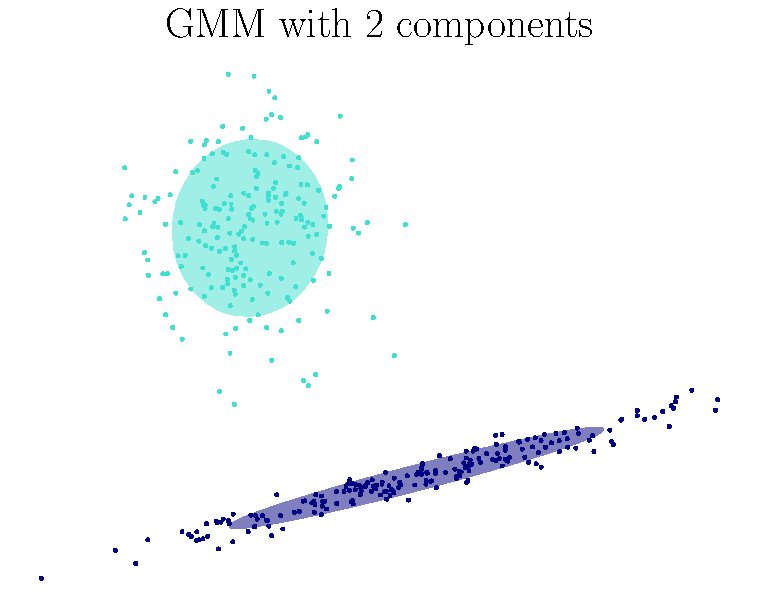
\includegraphics[page = 1, width=0.49\textwidth]{./figures/gmm}
\caption{Gaussian mixture model with two components. The equal probability surfaces are highlighted in colours.}
\label{fig:gmm}
\end{figure}
%------------------------------------------------------------

\section{Deep Generative Models}\label{sec:DGM}
We may regard the GMM as the simplest form of statistical generative model. Recent years have seen the advent of novel methods for generative modelling which we collectively refer to as Deep Generative Models (DGM), in complete analogy to what deep learning means with respect to machine learning. 
Before describing the most relevant forms of DGMs, and with no claim of completeness, we recall that some of the key features of deep learning include
\begin{itemize}
\item
models are parametrized by Neural Networks (NN) whose specific form depends on the particular task;
\item
the NN parameters are inferred via a stochastic gradient descent approach;
\item
in order to really exploit NNs, vast amount of high-fidelity data is needed for their training.
\end{itemize}
The last bullet is particularly attractive for LHC analysis, in that not only scientific collaborations such as ATLAS and CMS have already collected petabytes of data (with a lot more to come with the next upgrade of the collider), but we can also prepare data in a controlled environment for benchmarking models.

Concerning the practical realisation of DGMs, the three most successful frameworks studied and employed in the literature are
\begin{itemize}
\item
Normalizing Flows (NF~\cite{inn,coupling2,glow, nflow1,papamakarios2019normalizing,nflow_review,mller2018neural, grathwohl2018ffjord,chen2019neural});
\item
Generative Adversarial Networks (GAN)~\cite{goodfellow,Creswell2018, wgan_gp, wgan_original, lim2017geometric, zhang2019selfattention};
\item
Variational Autoencoders~\cite{kingma2014autoencoding,Kingma2019}.
\end{itemize}
The first two have been extensively employed in this thesis, and will be therefore further elaborated in the following sections.

\subsection{Normaling Flows}\label{intro:normflow}
Normalizing Flow  are defined in terms of a parametrized change of variable $G_{\theta}: z \rightarrow x$ between distributions
%
\begin{align}\label{eq:nf}
p_X(x) = p_Z(z) \left|\det \frac{\partial G_{\theta}(z)}{\partial z}\right|^{-1} = p_Z(\bar{G}_{\theta}(x)) \left|\det \frac{\partial \bar{G}_{\theta}(x)}{\partial x}\right|,
\end{align}
%
where $\bar{G}_{\theta} = G^{-1}_{\theta}$.
Regardless of how complicated $p_{X}(x)$ may be, if there exists a bijection $G_{\theta}$ such that $p_Z(z)$ is a simple distribution, e.g.\ a Gaussian $\mathcal{N}_{\mu=0, \Sigma=\mathbb{I}}$, we can draw samples from $p_{X}(x)$ via the generative pipeline
%
\begin{align}
z \sim p_Z(z) \longrightarrow x = G_{\theta}(z)  \sim p_{X}(x),
\end{align}
%
%
%------------------------------------------------------------
\begin{figure}[t]
\centering
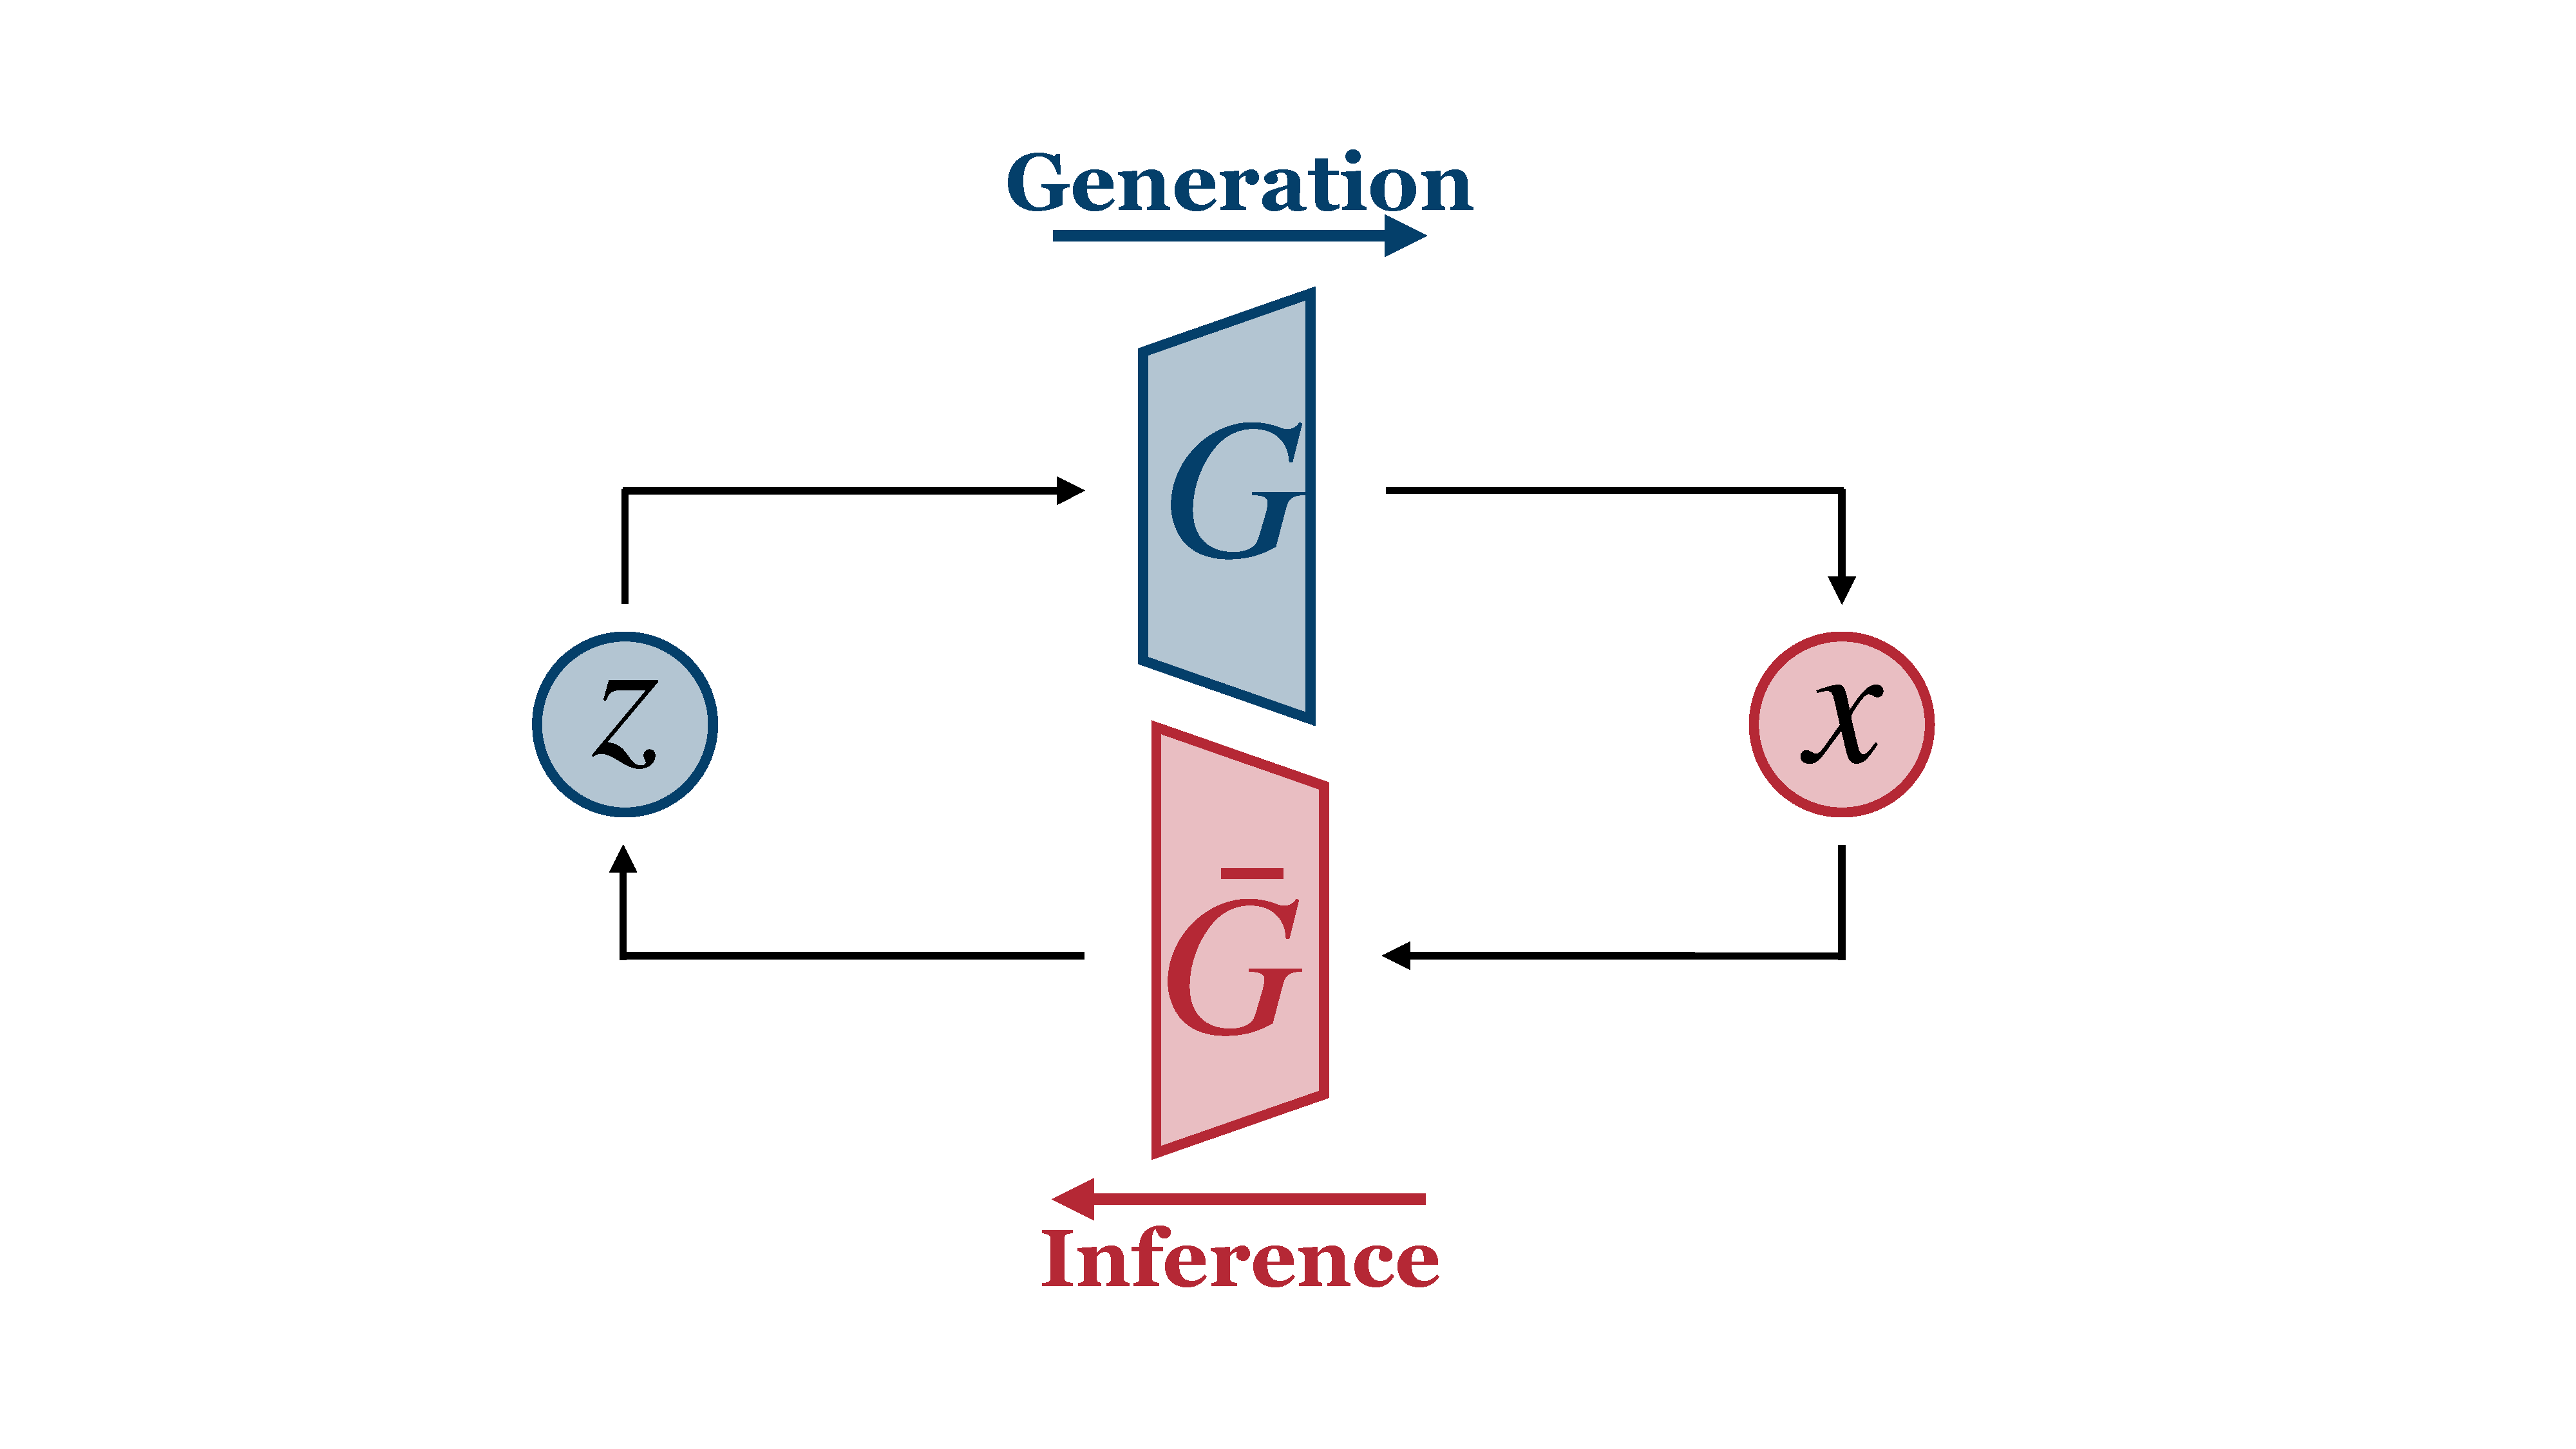
\includegraphics[page = 1, width=0.99\textwidth]{./figures/inn}
\caption{Schematic representation of a NF: a random variable $z$ sampled from a fixed, simple distribution is transformed via a map $G$ to a sample $x$ sampled from a complex target distribution. If $G$ is a bijection, and its inverse $\bar{G} = G^{-1}$ can be easily evaluated, the inverse direction can be used to train the model with Maximum Likelihood.}
\label{fig:NF}
\end{figure}
%------------------------------------------------------------
%
see Fig.~\ref{fig:NF} for a schematic representation. Similar to the GMM example in Sec.~\ref{sec:gmm}, the parameters of $G_{\theta}$ can be chosen to minimize the negative log-likelihood
%
\begin{align}\label{eq:change_of_variable}
\begin{split}
\mathcal{L} &= - \sum_{n=1}^N \log \left[ p_Z(\bar{G} _{\theta}(x_n)) \left|\det \frac{\partial \bar{G} _{\theta}(x)}{\partial x_n}\right| \right]\\
&= -\sum_{n=1}^N \log p_Z(\bar{G} _{\theta}(x_n)) + \log \left|\det \frac{\partial \bar{G} _{\theta}(x_n)}{\partial x_n}\right|\\
&= \sum_{n=1}^N \frac{(\bar{G} _{\theta}(x_n))^2}{2} - \log \left|\det \frac{\partial \bar{G} _{\theta}(x_n)}{\partial x_n}\right|,
\end{split}
\end{align}
%
where we have used $p_{Z}(z) = \mathcal{N}_{\mu=0, \Sigma=\mathbb{I}}$ and have discarded irrelevant constant terms. 
In practice, we only need to compute $\bar{G} _{\theta}(x_n)$, the corresponding determinant of the Jacobian, and minimize the combination in the final line of Eq.~\ref{eq:change_of_variable}.

This rather straightforward blueprint hides three complications one needs to carefully address. First of all, not only $G_{\theta}$ must be a bijection, i.e.\ its inverse must exist, but both $G_{\theta}$ and $\bar{G} _{\theta}$ must be efficiently computable, as one is required for training and the other for generating. Finally, the map must have a tractable Jacobian. If $G_{\theta}$ is parametrized by a standard NN, such as a Multi-Layer Perceptron (MLP), none of the three properties is satisfied. These constraints restrict the class of allowed transformations, limiting the expressive power at our disposal.
However, not all hope is lost, as we can build progressively more complex maps by simply stacking many simple functions, while maintaining the tractability of the Jacobian.
Given a bijection $G_{i}$ with inverse $\bar{G}_{i}$ and a cheap Jacobian, the composition
\begin{align}
G = G_{n} \cdot  G_{n-1} \ldots \cdot G_{1}
\end{align}
has inverse
\begin{align}
\bar{G} = \bar{G}_{1} \cdot   \ldots \cdot \bar{G}_{n-1} \cdot \bar{G}_{n},
\end{align}
and its determinant is the product of each individual determinant
\begin{align}
\det G = \prod_{i=1}^{N}  \det G_{i}.
\end{align}
This means that a composition of bijections is again a bijection whose computational complexity simply grows linearly with the number of compositions.
As a result, this research line is primarily dedicated to finding the optimal trade-off between computational complexity and model expressive power. 
In the remaining of this section we give an overview of past and currently used methods.

\subsubsection{Planar and Radial Flows}
The original work on NFs~\cite{pmlr-v37-rezende15} introduces the simple planar and radial flows. Despite representing seemingly simple transformations, they are not easily invertible.
A planar flow takes the form
%
\begin{align}
G(x) = x + u h(w^{T}x + b),
\end{align}
%
where $u, w, b$ are parameters and $h$ is a non-linear activation function. This transformation expands and contracts the distribution of $x$ along certain axis. The planar flow has the simple Jacobian
%
\begin{align}
\det \frac{\partial G}{\partial x} = 1 + h^{'}(w^{T}x + b) u^{T}w
\end{align}
%
which can be computed in $\mathcal{O}(D)$ time but cannot be inverted in closed form and its inverse does not exist in general.
Radial flows modify instead the distribution around a point $x_0$ as
%
\begin{align}
G(x) = x + \frac{\beta}{\alpha + ||x - x_0||}(x - x_0).
\end{align}
%
The same considerations apply here, the determinant of a radial flow can be efficiently computed, but its inverse is not always defined and cannot be computed in closed form.

\subsubsection{Dimensional Partitioning}

Introduced in ~\cite{coupling1, coupling2}, this approach builds an invertible transformation by splitting a $D$-dimensional input $x$ into two subspaces $(x_1, x_2)$, and defining the bijection $G$, normally called a coupling layer, as
%
\begin{align}
y_1 &= h(x_1, f(x_2))\\
y_2 &= x_2.
\end{align}
%
with inverse
%
\begin{align}
x_1 &= h^{-1}(y_1, f(y_2))\\
x_2 &= y_2.
\end{align}
%
The main feature of a coupling layer is that even if $f$ is an arbitrary function, the Jacobian of $G$ is always a triangular matrix which does not depend on the derivative of $f$. 
Different strategies can be used to perform the partitioning and ensure that every 
dimension gets transformed, such as alternating splittings in half and random 
permutations~\cite{coupling1}, using masked flow~\cite{coupling2} or using $(1 \times 1)$ convolutions~\cite{glow}. 
This is the method of choice for all the studies in this thesis, and in Chap.~\ref{chap:unfolding} we explain in details our implementation. 

\subsubsection{Autoregressive Flows}

An autoregressive flow is a non-linear generalization of a multiplication by a triangular matrix~\cite{kingma2017improving, papamakarios2018masked}. 
Motivated by the product rule of probability, stating that a joint density can be computed as a product of one dimensional conditionals
%
\begin{align}
p(x) = \prod_i p (x_i | x_{1:i-1}),
\end{align}
%
in an autoregressive model the output $y = G(x)$ is computed step-by-step as a function conditioned on the previous entries, i.e.\   
%
\begin{align}
y_t = h(x_t, f_t(x_{1:t-1})),
\end{align}
%
where $x_{1:t} = (x_1, \ldots, x_t)$, and $f_t$ is an arbitrary map taking a $t-1$ dimensional input. 
Similarly to a coupling layer, since each output $y_t$ only depends on $x_{1:t}$, the resulting Jacobian is again triangular and its determinant can be efficiently computed. The main difference with respect to coupling layers is that the inverse function, which can be trivially computed for the former, must be computed recursively as
%
\begin{align}
x_t = h^{-1}(y_t, f_t(x_{1:t-1})).
\end{align}
%
As this operation is inherently sequential, it cannot be parallelized and represent therefore a bottleneck for training this kind of model. Depending on the application, one may want to either have a fast forward direction, in which case one gets a so called masked autoregressive flow, or a fast inverse direction, giving instead an inverse autoregressive flow.

\subsubsection{Residual Flows and ODE}

The last method we present is based on residual connections, i.e.\  maps with the form
%
\begin{align}
G(x) = x + f(x).
\end{align}
%
Residual blocks have been used for a long time~\cite{he2015deep}, and have been adapted into invertible architecture in Ref.~\cite{gomez2017reversible, jacobsen2018irevnet}. Splitting input and output as $(x_1, x_2)$, $(y_1, y_2)$, the map
%
\begin{align}
y_1 &= x_1 + f(x_2)\\
y_2 &= x_2 + l(y_1)
\end{align}
%
is trivially invertible, but has an inefficient Jacobian. Ref.~\cite{gomez2017reversible, jacobsen2018irevnet} introduces
strategies to enforce the invertibility.
Most notably, however, is the fact one can see a residual connection as the discretized 
version of an ordinary differential equation. 
The starting point is an ordinary differential equation of the form
%
\begin{align}\label{eq:ode}
\frac{d}{dt}x(t) = F(x(t), \theta(t)),
\end{align}
%
where $F : \mathbb{R}^D \times \Theta \rightarrow \mathbb{R}^D$ encodes the dynamics of the system, $\Theta$ is a set of parameters and $\theta : \mathbb{R} \rightarrow \Theta$ is a parametrization.
The discrete version of Eq.~\ref{eq:ode} 
%
\begin{align}
x_{n+1} - x_n = \epsilon F(x_n, \theta_n), 
\end{align}
%
is equivalent to the equation of a residual connection with residual block $\epsilon F$.
Starting from this intuition, Ref.~\cite{dupont2019augmented, chen2019neural , grathwohl2018ffjord} 
propose to directly solve the continuous version Eq.~\ref{eq:ode}, which in this differential equation picture 
would correspond to training an infinitely deep network.

\medskip

We conclude this section with a comment motivating the study of Chap.~\ref{chap:lsr}. As already stated, invertible models are bijections, or homeomorphisms~\cite{dupont2019augmented,  huang2020augmented} (note that this is a strict equivalence, i.e.\   an invertible model does not approximate a homeomorphism, it is one), and as such they are by construction unable to map manifolds with different topological features, such as the number of holes and disconnected patches. In particular, if we stick to the standard formulation and only consider Gaussian latent spaces, we may only be able to represent data whose underlying manifold is compact and has genus zero. As this may be a limiting factor for the naive use of normalizing flows in particle physics, in Chap.~\ref{chap:lsr} we illustrate a possible method to account for it.

\subsection{Generative Adversarial Networks}\label{intro:gan}
GANs introduce a brand new paradigm for generative modelling which, unlike the previously described methods, doesn't involve computing the likelihood at all, and is therefore a form of likelihood-free machine learning. Instead, GANs rely on a two-sample test between distributions, i.e.\   a statistical test to determine whether or not two samples are drawn from the same distribution. This test is formulated as a differentiable objective function so that it can be minimized with stochastic gradient descent methods, in such a way that it is minimal iff the two distributions are statistically identical.
The statistical test is performed by a discriminator $D_{\phi}$ whose job is to tell apart real and fake samples. The final piece of a GAN is a generator $G_{\theta}$, a map from noise $z$ to target samples $\tilde{x}$, see Fig.~\ref{fig:gan}. In DL, both $D_{\phi}$ and $G_{\theta}$ are properly shaped NNs.
%
%------------------------------------------------------------
\begin{figure}[t]
\centering
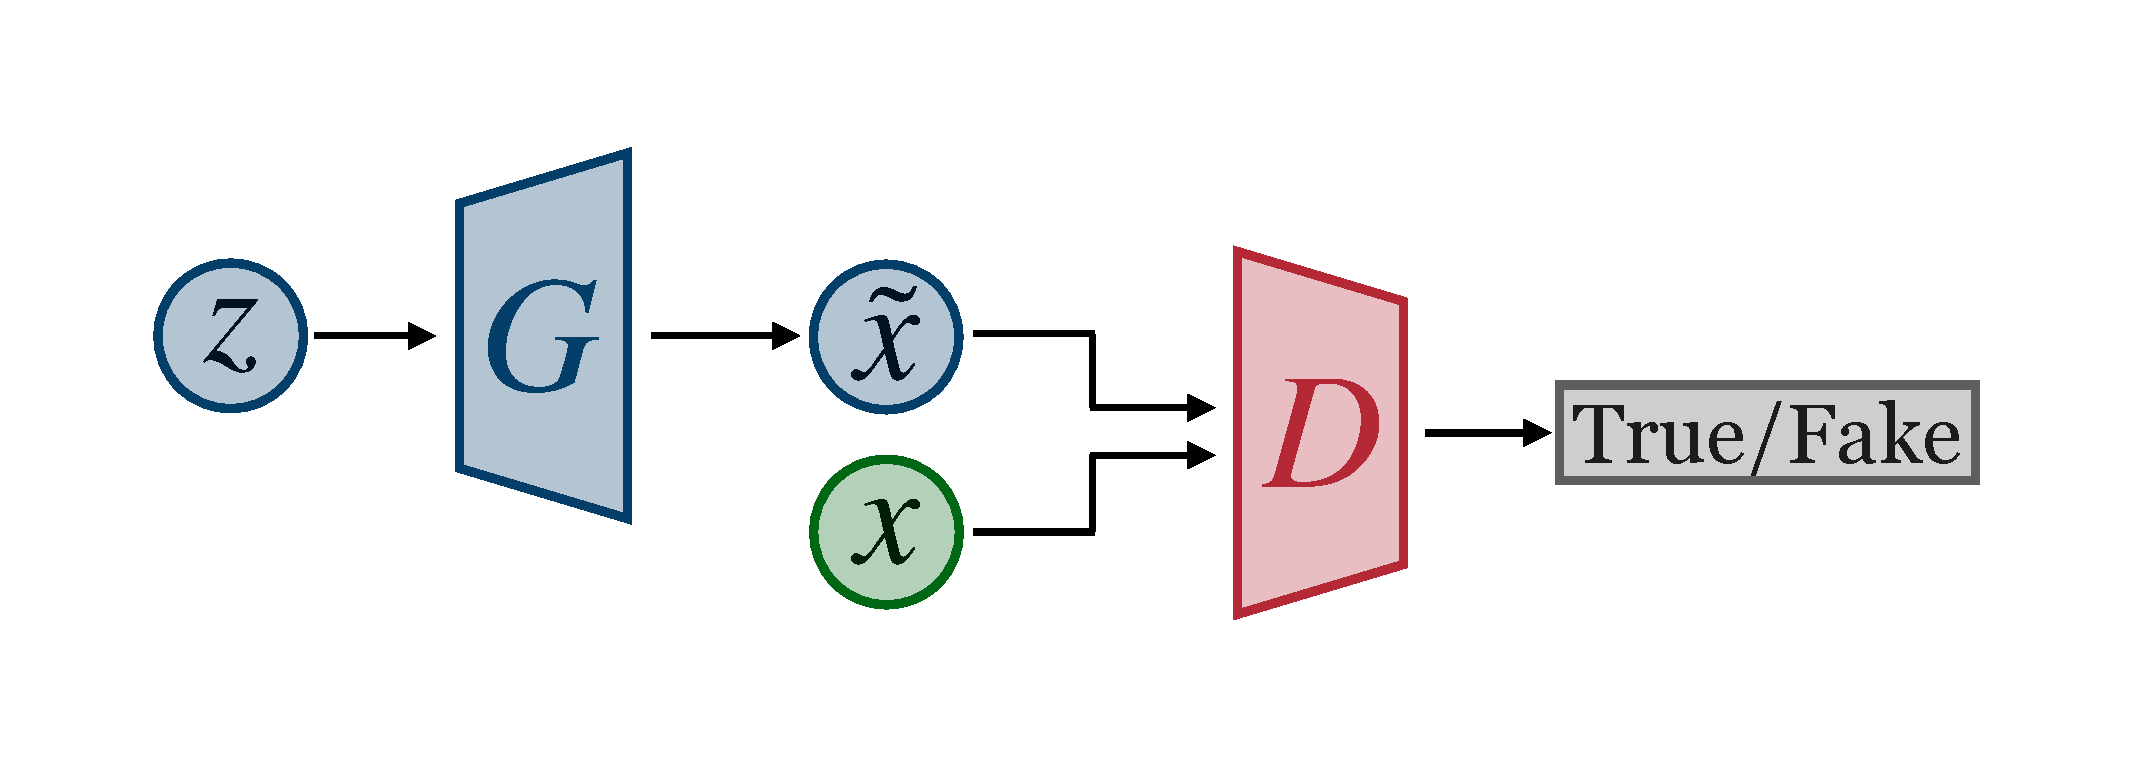
\includegraphics[page = 1, width=0.99\textwidth]{./figures/gan}
\caption{Schematic representation of a GAN: a generator $G$ deterministically maps noise $z$ to fake samples $\tilde{x}$. The discriminator $D$ is trained as a binary classifier of true versus fake data, while $G$ tries to fool it.}
\label{fig:gan}
\end{figure}
%------------------------------------------------------------
%
While many different ways to define the GAN objective have been proposed, we refer to the original formulation\cite{goodfellow} as it is close to the one employed in Chap.~\ref{chap:unfolding}. Formally, we consider the min-max game 
%
\begin{align}
\min_{\theta} \max_{\phi}\mathbb{E}_{x \sim p_{X}(x)} \left[ \log D_{\phi} (x) \right] + \mathbb{E}_{z\sim p_{Z}(z)} \left[ \log \left( 1 - D_{\phi} (G_{\theta}(z) \right) \right].
\end{align}
%
For a fixed generator, this is nothing other than a binary classification task, and an optimal discriminator should output $1$ for any $x \sim p_{X}(x)$ and $0$ otherwise, which we can summarize as
%
\begin{align}
D_{\phi^{*}}(x) = \frac{p_{X}(x)}{p_{X}(x) + p_{G}(x)},
\end{align}
%
with $p_{G}(x)$ being the distribution implicitly defined by the generator. 
Fixing $\phi = \phi^{*}$, the generator part of the objective is equivalent to minimizing the Jenson-Shannon divergence $JS(p_{X}, p_{G})$, with
%
\begin{align}
JS\left(p, q\right) = \frac{1}{2} \left(KL\left(p, \frac{p + q}{2}\right) + KL\left(q, \frac{p + q}{2}\right) \right),
\end{align}
%
and $KL(a, b)$ is the Kullback-Leibler divergence between $p$ and $q$. This objective has a global minimum for $p_{G} = p_{X}$.
It turns out that if the discriminator is optimal, the objective function has vanishing gradient for the generator, leading to the standard alternating training of GANs: every $k$ updates of $\phi$ we perform an update of $\theta$, $k$ being a hyperparameter.
Training a GAN is a highly non trivial task with many potential issues if extra care is not taken, notably
\begin{itemize}
\item
the optimization procedure is typically unstable and needs to be regularized;
\item
for multi-modal targets, generators can collapse to a single mode;
\item
since the objective function is not convex, there is no clear way to evaluate the model performances or to determine a stopping point.
\end{itemize}
%Plenty of empirical tips and tricks to stabilize the training of GANs are available in the literature, in the form of modified objective functions, gradient penalties, noise injection, specific optimizers and more.

An important difference between the two presented frameworks is that a GAN represents a target density only implicitly, i.e.\    $G_{\theta}$ is only a sampler from $p_{X}$, but can't be used to estimate its value (with the exception of low dimensional problems where kernel methods may be used to smooth a binned distribution). On the other hand, the explicit value of the density can be trivially computed with a NF from Eq.~\ref{eq:nf} if we assume a perfect map to the latent space distribution.

\section{Unfolding}\label{intro:unfolding}

In any quantitative science we wish to be able to estimate the possible value of "true" parameters, directly connected to some underlying theory, given that we are only able of observing a distorted version of them in the best scenario, more realistically we will have to be satisfied with observing a different set of parameters entirely.
In particular, we are often interested in lifting the effects induced by the detectors and possible physical and theoretical backgrounds. This procedure is normally called de-convolution, and takes the name of unfolding in particle physics. In this section we first revise a standard method for unfolding based on Bayesian inference, and then illustrate how to set-up a deep-learning version of it.

\subsection{Iterated Bayesian Unfolding}
In this section we will define the fundamental ideas of unfolding following closely Ref.~\cite{DAgostini:1994fjx, dagostini2010improved}.
Bayesian inference is a framework to estimate unknown parameters from observed data. A starting point for Bayesian unfolding is the discretization of the problem, in the form of binning of observable distribution of events, with each bin being treated as an independent variables.
%
%------------------------------------------------------------
\begin{figure}[t]
\centering
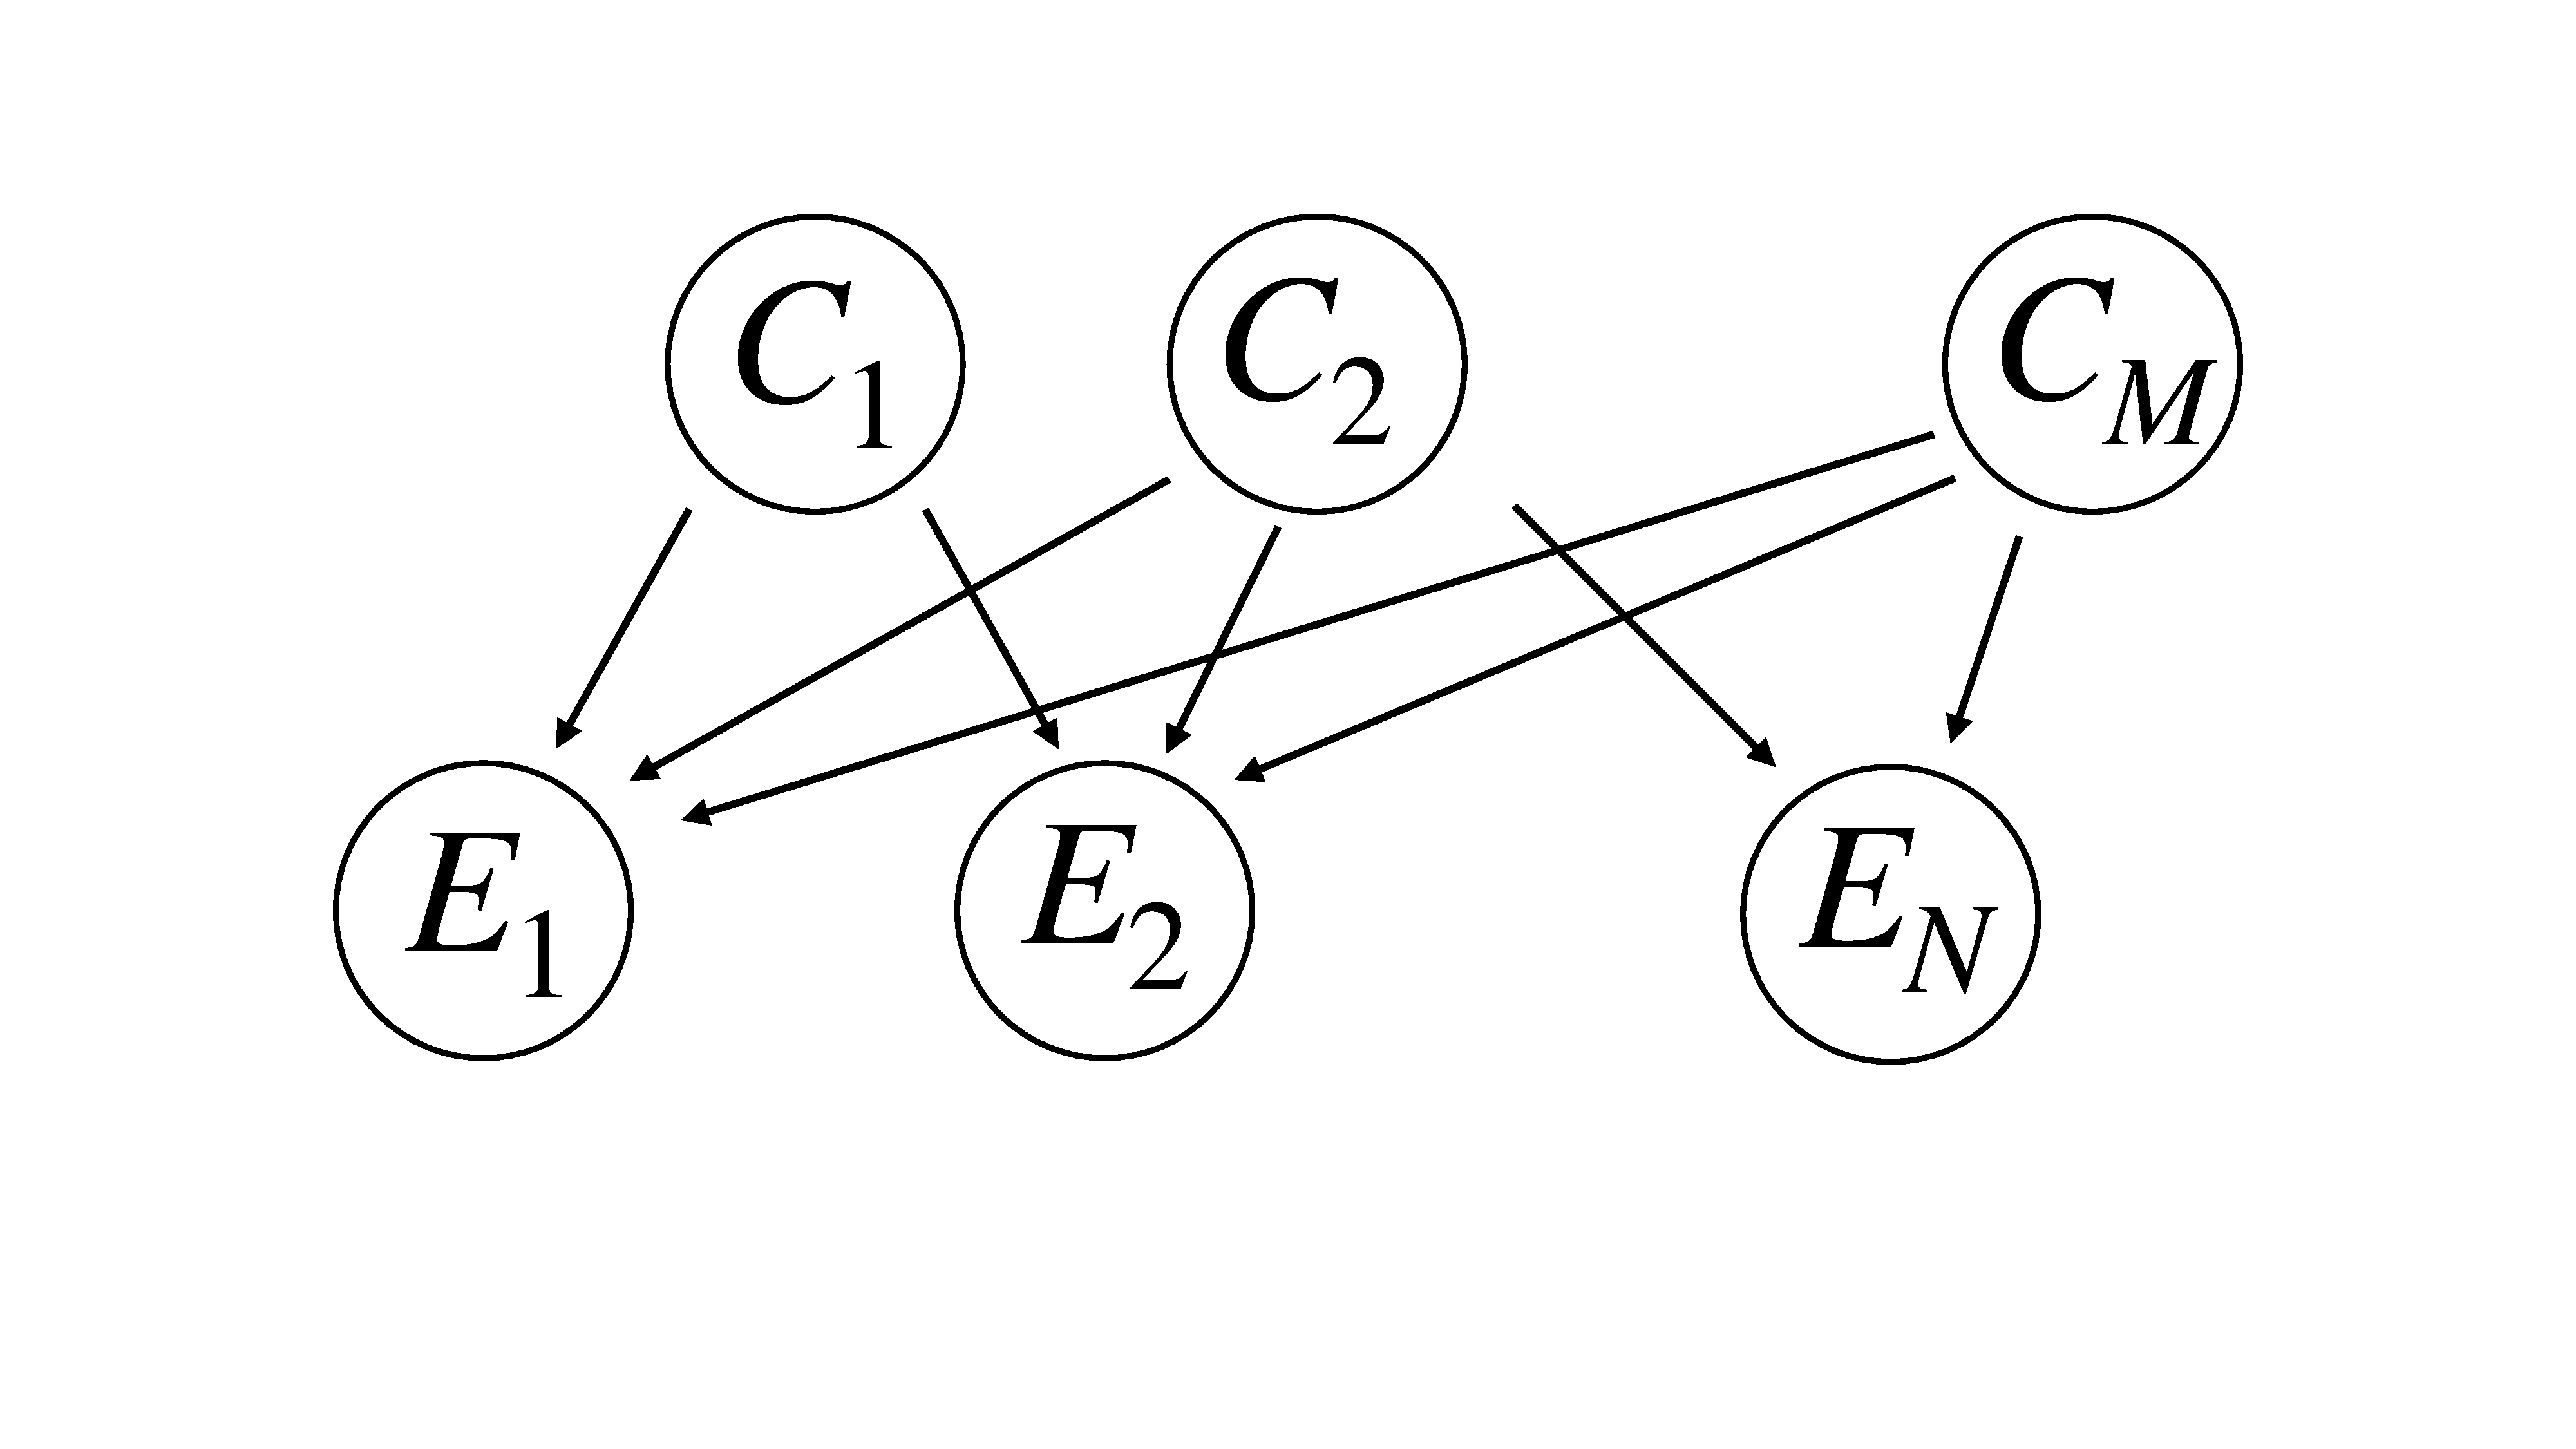
\includegraphics[page = 1, width=0.95\textwidth]{./figures/graphical_model}
\caption{Graphical model of causes and effects. Each arrow represents a probabilistic link}
\label{fig:graph_model}
\end{figure}
%------------------------------------------------------------
%
Borrowing the language of graphical models, the problem can be described by the Bayesian network of Fig.~\ref{fig:graph_model}, $C_{i}$ being the true number of events in each cause bin, given that we observe $E_{j}$ events per bin.
It's important to notice that as the links between cause and effect is probabilistic, so will be the number of true events per bin. Concretely,  given causes $C_i$ and effects $E_j$, we wish to estimate the conditional distribution
%
\begin{align}\label{eq:unf}
P(C_i | E_j)
\end{align}
%
Following standard Bayesian inference, Eq.~\ref{eq:unf} may be computed as
%
\begin{align}\label{eq:bayes_inf}
P(C_i | E_j) = \frac{P(E_j | C_i) P(C_i)}{\sum_{l=1}^{n_E} P(E_j| C_l) P(C_l)},
\end{align}
Eq.~\ref{eq:bayes_inf} is Bayes' theorem stating that the posterior is proportional to the likelihood, provided that we multiply by the prior
%
\begin{align}
P(C_i | E_j) \propto P(E_j | C_i) P(C_i),
\end{align}
%
and the denominator is a normalization factor.
%The main issue in the practical application of Eq.~\ref{eq:bayes_inf} is that there is no closed to compute 
The unfolding algorithm proceeds as follows:
\begin{itemize}
\item
estimate the number of expected events in bin $C_i$ given that $n(E_i)$ is the observed counting bin $E_j$\\
\begin{align}
n(C_i)|_{n(E_j)} \sim P(C_i | E_j) n(E_j);
\end{align}
\item
include effects from all observations\\
\begin{align}
n(C_i) = \sum_j P(C_i | E_j) n(E_j);
\end{align}
\item
correct for the effect of different efficiencies $\epsilon_i$\\
\begin{align}\label{eq:IBU}
\tilde{n}(C_i) = \frac{1}{\epsilon_i} n(C_i) = \frac{1}{\epsilon_i}\sum_{j=1}^{n_E} P(C_i | E_j) n(E_j);
\end{align}
with the efficiencies computed from the smearing matrix as
\begin{align}
\epsilon_i = \sum_{j=1}^{n_E} P(E_j | C_i) = \sum_{j=1}^{n_E} \lambda_{ij},
\end{align}
where $\lambda_{ij} = P(E_j | C_i)$ are the entries of a smearing matrix $\Lambda$ estimated from Monte Carlo simulations. 
\end{itemize}

The above algorithm is essentially the first form of Bayesian unfolding presented in Ref.~\cite{DAgostini:1994fjx}. Ref.~\cite{dagostini2010improved} introduced several improvements over the first version. A first improvements concerns the explicit modelling of the smearing matrix. In the original formulation, one starts by generating a large number of events in each cell and counting where they end up after the simulation. The entries $\lambda_{ij}$ are estimated as
%
\begin{align}
\lambda_{ij} \sim \frac{n(E_j)^{MC}}{n(C_i)^{MC}}.
\end{align}
%
We can both improve this estimate, and include its uncertainty, by employing again Bayes theorem and computing a posterior over the $\lambda_{ij}$. Given a column $\lambda_i$ of $\Lambda$, we have
%
\begin{align}
f(\lambda_i | n(E)^{MC}, n(C_i)^{MC}) \propto P(n(E)^{MC} | n(C_i)^{MC}, \lambda_i) f(\lambda_i).
\end{align}
%
If we choose a Dirichlet prior for $\lambda_i$ it is possible to show
%
\begin{align}
\lambda_i \sim \text{Dir}(\alpha_{\text{posterior}, i}), \quad \alpha_{\text{posterior}, i } = \alpha_{\text{prior}, i} + n(E)^{MC}|_{n(C_i)^{MC}},
\end{align}
%
where
%
\begin{align}
\text{Dir}(x | \alpha) = x_1^{\alpha_1 -1 } \ldots x_n^{\alpha_n -1 }.
\end{align}
%
We can now account for the extra uncertainty in $P(C_i | E_j)$ by computing
%%
%\begin{align}
%f(x | \alpha) = \frac{\Gamma(\alpha_1 + \ldots + \alpha_n)}{\Gamma(\alpha_1) \ldots \Gamma(\alpha_n)} x_1^{\alpha_1 -1} \ldots x_n^{\alpha_n -1}
%\end{align}
%%
%
\begin{align}
P(C_i | E_j) \longrightarrow P(C_i | E_j, \Lambda); \qquad P(C_i | E_j) = \int P(C_i | E_j) f(\Lambda) d\Lambda,
\end{align}
%
i.e.\ the posterior over causes depends explicitly on the smearing matrix $\Lambda$, which is sampled from the posterior distribution $f(\Lambda)$.
Most notably, however, is the additional iteration of the algorithm. Bayesian inference only makes sense when we have a prior belief of what the possible values of the unobserved parameters are. Choosing a "correct" prior is a tricky task, as this choice, which is arbitrary, affects the posterior distribution.
Ref.~\cite{dagostini2010improved} suggests that the dependence on the prior can be reduced by iterating the unfolding procedure, by using the result of unfolding step $n$ as the prior of unfolding $n+1$. This method is therefore called Iterated Bayesian Unfolding (IBU).

We conclude the introduction with a brief discussions of the limitations of iterated Bayesian unfolding, and equivalent methods. The first obvious limitation is that the method relies on binning measurements into histograms. Binning can be problematic as aside with the exception of few limited case there's no obvious best binning, and each individual observable typically requires an ad hoc manual choice of the binning. Directly related to this is the fact that the total number of bins grows exponentially with the number of dimensions, each being a different observable. This means that differential cross section measurements beyond a few dimensions are impractical.

\subsection{OmniFold}

In parallel to the work of Ref.~\cite{cond_gan, Bellagente:2020piv}, which constitutes the main content of Chap.~\ref{chap:unfolding}, another deep-learning framework for unfolding has been published. Because of its relevance as the only other existing method for unfolding relying on deep-learning, and for its connection to IBU, we believe that an explanation of the \textsc{OmniFold} method~\cite{Andreassen:2019cjw} deserves its own section.

\textsc{OmniFold} has been proposed to overcome the two main shortcomings of IBU, binning and handling multiple dimensions, by generalizing the iterated version of Eq.~\ref{eq:IBU} to the continuous, multi-dimensional case. In Fig.~\ref{fig:omnifold} we illustrate schematically the method.
%
%------------------------------------------------------------
\begin{figure}[t]
\centering
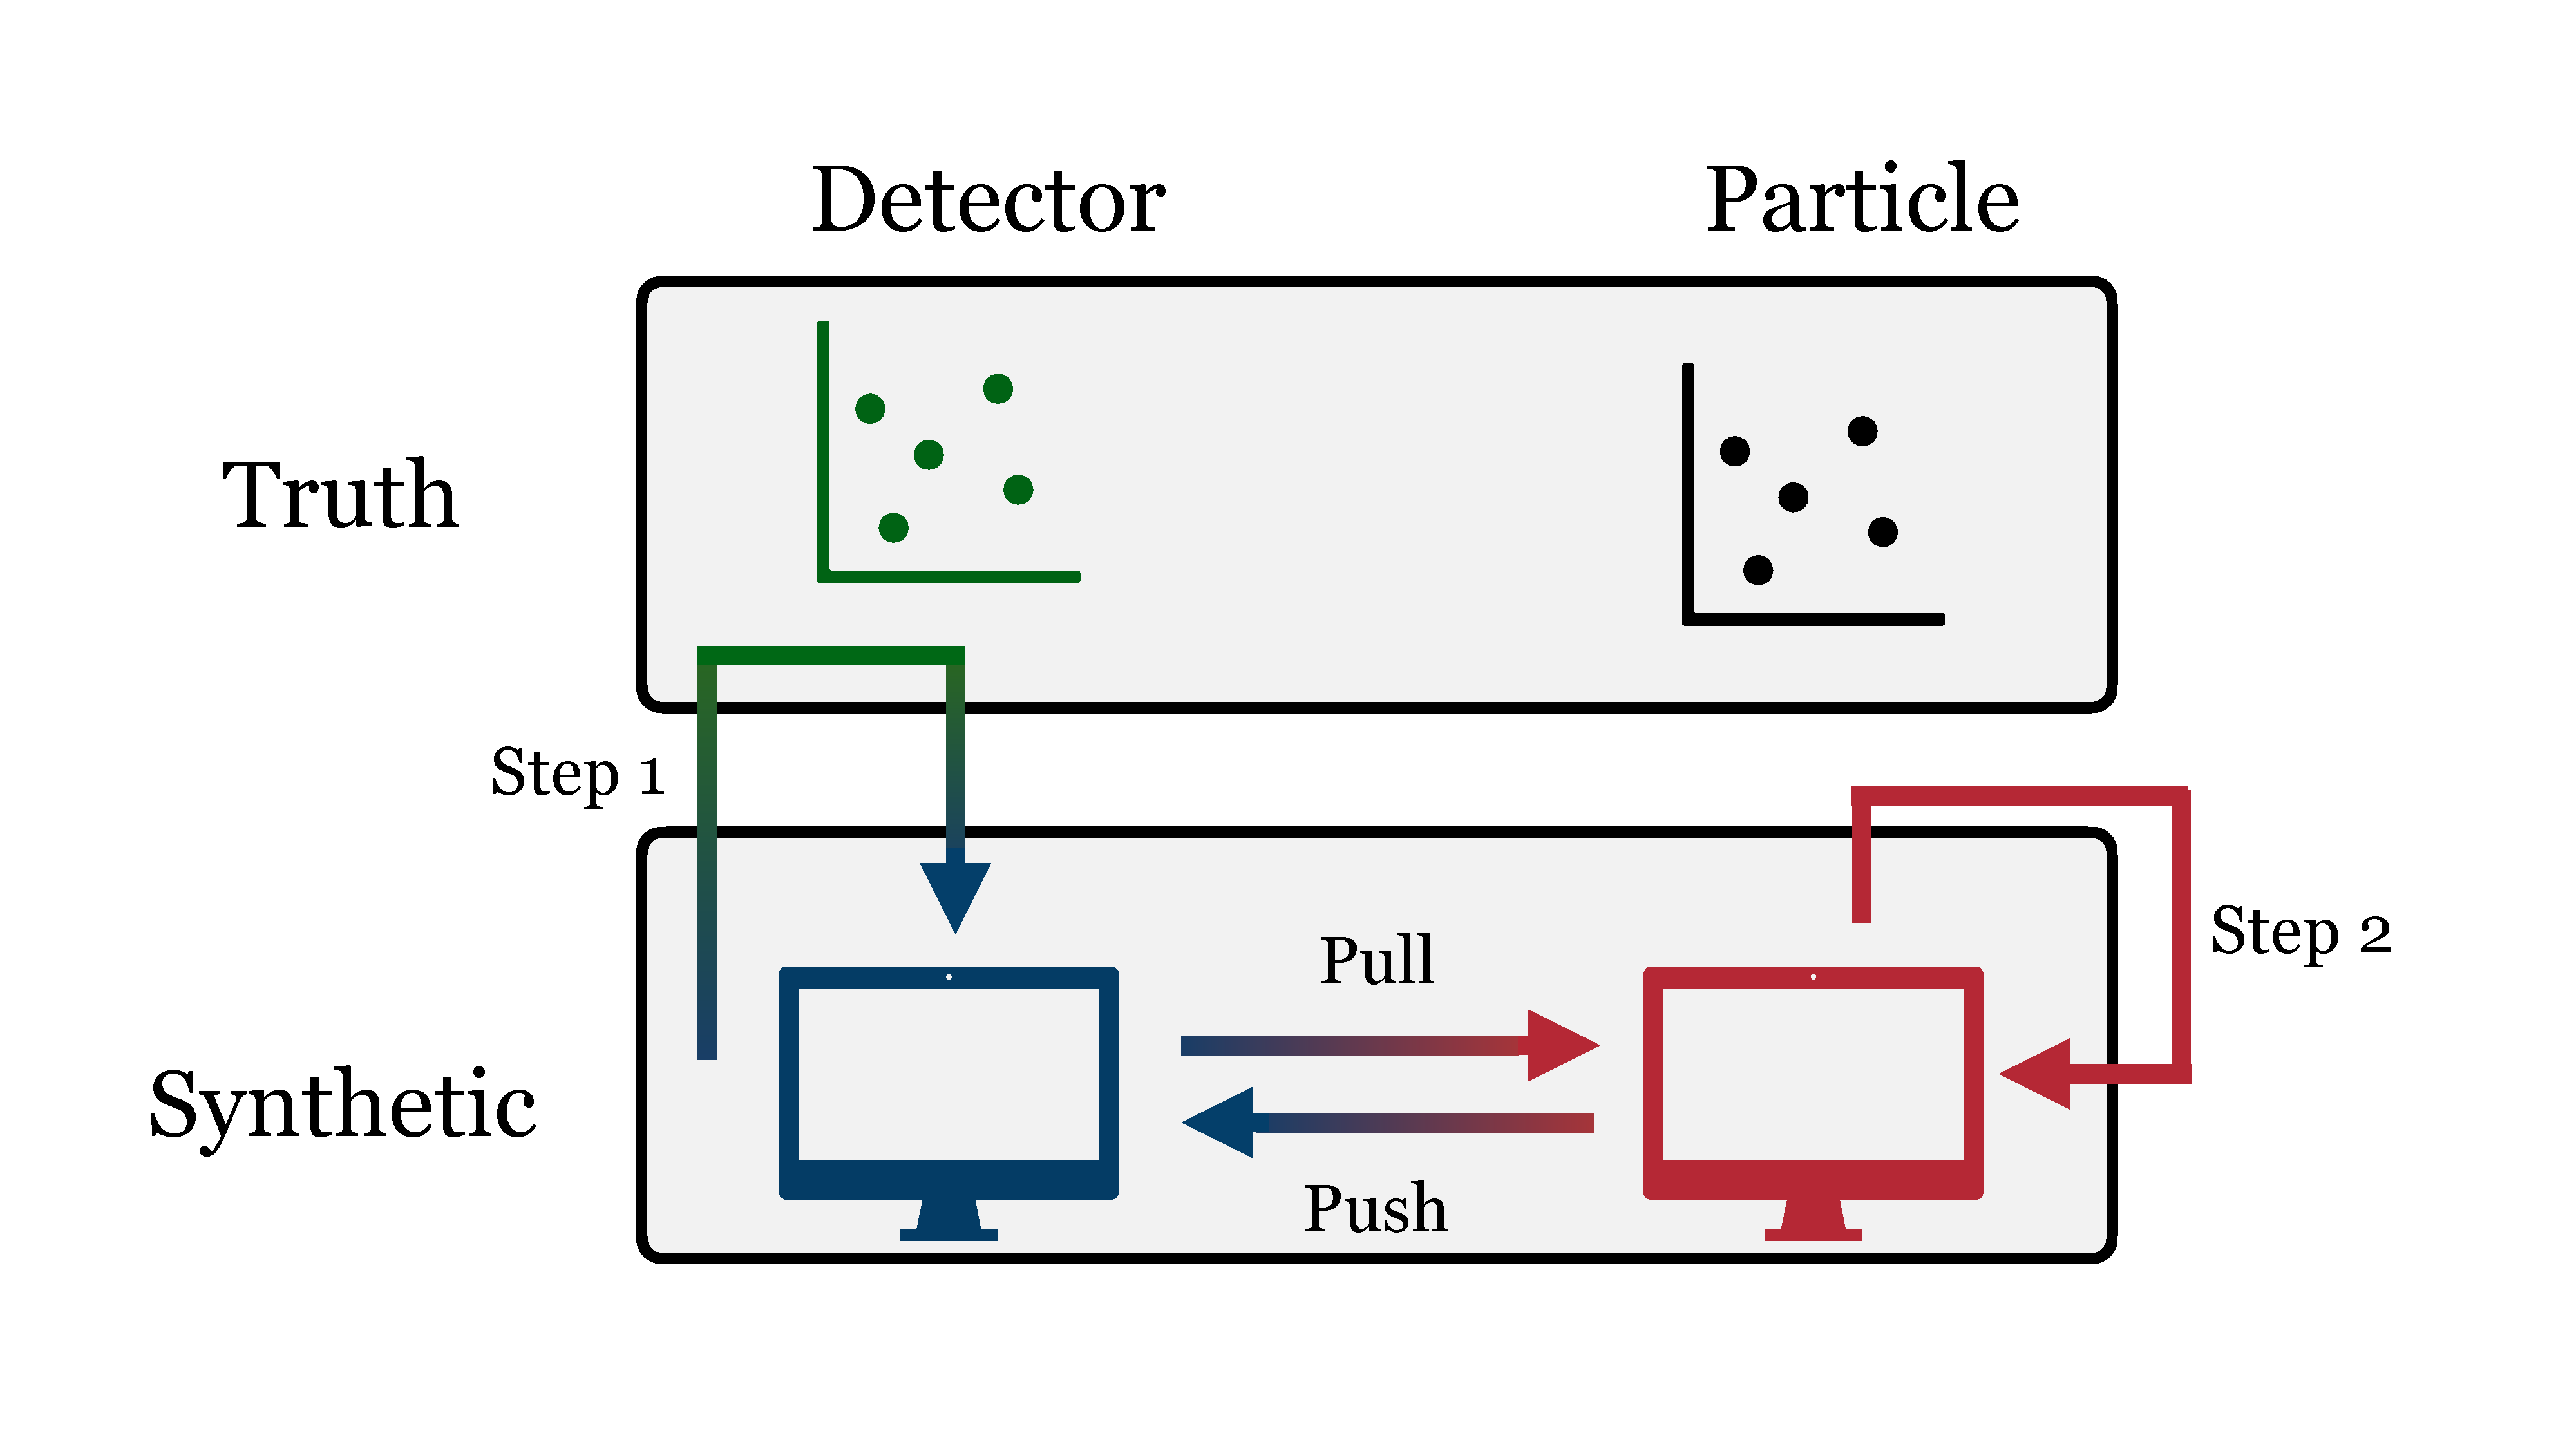
\includegraphics[page = 1, width=0.95\textwidth]{./figures/omnifold}
\caption{Illustration of the \textsc{OmniFold} method: synthetic data is reweighted against the true data at the detector level. This weights are pulled back at the particle level to induce weights on the particle level data. In the second step the original synthetic particle level data is weighted to match its reweighted version. The process is then iterated.}
\label{fig:omnifold}
\end{figure}
%------------------------------------------------------------
%
Starting with particle level events $t$ with initial weights $\nu_0(t)$ simulated with Monte Carlo, we produce a paired set of detector level events $m$ with induced weights $\nu_0^{\text{push}}(m) = \nu_0(t)$.
We then compute new weights $\omega_0(m)$, and use them to obtain the next set of particle level weights $\nu_1(t)$. The key idea to achieve the correct reweighting is that the likelihood ratio
%
\begin{align}
L \left[ (w, X), (w^{'}, X^{'}) \right](x) = \frac{p_{w, X}(x)}{p_{w^{'}, X^{'}}(x)},
\end{align}
%
can be approximated using a classifier trained to distinguish $(w, X)$ against $(w^{'}, X^{'})$~\cite{Andreassen:2019nnm, brehmer1, brehmer2, mining, cranmer2016approximating}.
With the likelihood ratio it is straightforward to reweight events as
\begin{align}
\omega_n(m) = \nu_{n-1}^{\text{push}} L \left[ (1, \text{truth, det)}), (\nu_{n-1}^{\text{push}}, \text{Synt, det)})\right],\\
\nu_n(t) = \nu_{n-1} L \left[ (\omega_n, \text{synt, part)}), (\nu_{n-1}, \text{synt, part)})\right].
\end{align}
It is possible to show that after one iteration the new weights are given by
%
\begin{align}
\nu_1 p_{synt, part}(t) = \int dm^{'} p_{\text{ synt, part| Synt, Det}} (t | m^{'}) p_{\text{truth, det}}(m^{'})
\end{align}
%
which is a continuous version of Eq.~\ref{eq:IBU}. On top of that, \textsc{OmniFold} is not limited by the dimensionality of the observables, and can in principle unfold the full phase space of an event, provided that the classifier employed is powerful enough.

%\documentclass[a4paper,twoside,10pt,openright]{report}%Dokumentenklasse 
\usepackage{graphicx} %Compiler

\usepackage{dsfont}

%%%% Schrift und Kodierung %%%%
	\usepackage[T1]{fontenc} %Zeichensatzkodierung von 7bit auf 8bit 
	\usepackage[utf8]{inputenc} %Zeichensatzkodierung Unicode bzw. UTF8
	\usepackage{lmodern} %Vektorschrift
	%\RequirePackage[english,spanish,es-nolayout]{babel}
	\usepackage[english]{babel}
	\usepackage{textcomp}
	\usepackage{lmodern}
	\usepackage{url}
	\usepackage[bookmarksnumbered=true]{hyperref}
    \graphicspath{{figures/}}	
	
%%% COLORS %%%
\newcommand{\hl}[1]{
   \textcolor{MidnightBlue!90!black}{#1} 
}

\usepackage{pifont}% http://ctan.org/pkg/pifont
\newcommand{\cmark}{\ding{51}}%
\newcommand{\xmark}{\ding{55}}%

\usepackage{stackrel}

\usepackage{feynmp}

\usepackage{amsthm}
\newtheorem{definition}{Definition}
\newtheorem{proposition}{Proposition}
	
%%%% Fancy Header %%%
\usepackage{fancyhdr}
\usepackage[dvipsnames]{xcolor}
\usepackage{tikz} 
\usepackage{pgfplots}
%\usepackage{pgf-pie}

\usetikzlibrary{arrows}
\usetikzlibrary{shapes.geometric, arrows}

\definecolor{mycolor}{rgb}{0.45,0.45,0.45}% dark grey

\newcommand{\mcD}{\mathcal{D}}
\newcommand{\mcL}{\mathcal{L}}
\newcommand{\dth}{\Delta_{\text{th/sys}}}
\newcommand{\dst}{\Delta_{\text{stat}}}
\newcommand{\dsy}{\Delta_{\text{syst}}}
\newcommand{\sthsy}{\sigma_{\text{th/sys}}}
\newcommand{\sth}{\sigma_{\text{th}}}
\newcommand{\sst}{\sigma_{\text{stat}}}
\newcommand{\ssy}{\sigma_{\text{syst}}}

\newcommand{\Langle}{\big\langle}
\newcommand{\Rangle}{\big\rangle} 
 
\fancyhf{}
\fancyhead[LE]{\sffamily\color{mycolor}\nouppercase{\leftmark}} % left even, right odd
\fancyhead[RO]{\sffamily\color{mycolor}\nouppercase{\rightmark}} % left even, right odd
\fancyfoot[CE,CO]{\sffamily\color{mycolor}\nouppercase{\thepage}} % center even, center odd
\renewcommand{\headrule}{{\color{mycolor}%
\hrule width\headwidth height\headrulewidth \vskip-\headrulewidth}}
\renewcommand{\headrulewidth}{0.5pt}

\fancypagestyle{plain}{%
    \fancyhf{}%
    \fancyfoot[CE,CO]{ { \sffamily\color{mycolor}{\thepage} } }
	\renewcommand{\headrulewidth}{0.0pt}
}

%\fancypagestyle{fancy}{%
%   \fancyhf{}
%	\fancyhead[LE,RO]{\sffamily\color{mycolor}\nouppercase{\leftmark}} % left even, right odd
%	\fancyfoot[CE,CO]{\sffamily\color{mycolor}\nouppercase{\thepage}} % center even, center odd
%	\renewcommand{\headrule}{{\color{mycolor}%
%	\hrule width\headwidth height\headrulewidth \vskip-\headrulewidth}}
%	\renewcommand{\headrulewidth}{0.5pt}
%}


%%% Customize titles %%%%
\usepackage[ ]{titlesec}  %
\usepackage{etoolbox}
\makeatletter
\patchcmd{\ttlh@hang}{\parindent\z@}{\parindent\z@\leavevmode}{}{}
\patchcmd{\ttlh@hang}{\noindent}{}{}{}
\makeatother
%\titleformat{\chapter}[display]
%  { \normalsize \huge  \color{black}}%
%  {\flushright \normalsize \color{mycolor} \MakeUppercase %
%  {\sffamily \chaptertitlename } \hspace{1 ex}%
%  { \fontsize{60}{60}\selectfont \color{mycolor} \sffamily  \thechapter }}%
%  {10 pt}%
%  {\sffamily \huge \color{mycolor}\bfseries}
%\newcommand\mychapformat[1]{\parbox[t]{\dimexpr\textwidth-3em\relax}{\raggedleft#1}}
\titleformat{\chapter}[hang]{\Huge\bfseries\color{mycolor}\sffamily}% the number
	{\thechapter\hspace{20pt}\textcolor{mycolor}{|}\hspace{20pt}}%
	{0pt}{\Huge\bfseries\color{mycolor}\sffamily}% the title
\titleformat*{\section}{\sffamily\LARGE\color{mycolor}}
\titleformat*{\subsection}{\sffamily\Large\color{mycolor}}
\titleformat*{\subsubsection}{\sffamily\large\color{mycolor}}
\titleformat*{\paragraph}{\sffamily\large\bfseries\color{mycolor}}



	
%%%% Mathepakete %%%%
	\usepackage{array}
	\usepackage{calc}
	\usepackage{amsmath}
	\usepackage[intlimits]{empheq}
	\usepackage{amssymb,mathrsfs}
	\usepackage{theorem}
	\usepackage{slashed}
	\usepackage{feynmp-auto}

%%%% Sonstiges %%%%
	%\usepackage{subcaption}
	\expandafter\def\csname ver@subfig.sty\endcsname{}
	\usepackage{subfig} %Ermöglicht subfloats, also mehrere Tabellen/Bilder in einer Umgebung
	\usepackage{float} %Setzt mit [H] Figuren genau dort hin, wo sie im Text auftauchen
	\usepackage{booktabs} %Andere Tabellen
	\usepackage{gensymb}
	\usepackage{extarrows}%lange Pfeile
%	\usepackage{pst-pdf}	
	\usepackage{wasysym} %Symbolpaket
	\usepackage{multirow} %Ein Wert für mehrere Zeilen oder Spalten von Tabellen. Verwendung \multirow{#AnzahlZeilen}{*}{Name} bzw. analog \multicolumn{}{}{}
	\usepackage{rotating} %ermöglicht Schiefe Schrift
	%\usepackage{ziffer} %Deutsche Zahlen (Komma als Dezimalstelle im Mathemodus!)
	\usepackage{nicefrac} %Im Text schöne Brüche
	\usepackage[inner=3cm, outer=2.4cm, top=3cm]{geometry} %Passt Seitenränder an (left, right, top, bottom, width, height, textwidth, textheight)
	\usepackage{scrhack} %Verbessert angeblich LaTeX-Pakete
	\usepackage{numprint} %ROOT-Zahlen in deutsches zahlenformat übertragen. Syntax: \numprint[kg]{1.234e56} wird zu 1,234 * 10^56 kg
	\usepackage{cite}
	\usepackage{placeins}
	\usepackage{changepage}
	%\hyphenation{con-fine-ment}
	
%%%% spezielle Formatierungen %%%%
	\setlength{\emergencystretch}{25pt} %verhindert das Herausragen von Wörtern übers Zeilenende
	\setlength{\parindent}{0pt} %Kein Einschub bei neuem Absatz
	\setlength{\parskip}{2pt plus 1pt} %Erhöht Abstand zwischen Absätzen (um 1pt flexibel bei Seitenumbrüchen)
	
	%%%% Dokument-Variablen %%%%
\date{\today}

%%%% Eigene Befehle %%%%
\DeclareGraphicsRule{*}{mps}{*}{}
	\newcommand{\mE}[1]{\,\mathrm{#1}} %Einheiten im Mathemodus
	\renewcommand{\sl}[1]{\slashed{#1}} %Feynman-Slash
	\newcommand{\dummyImage}[2]{  %Erzeugt eine Umgebung wie includegraphics
		\frame{\mbox{\rule{0pt}{#2}	Bild fehlt  noch \rule{#1}{0pt}}}
	}
	\renewcommand{\i}{\mathrm{i}} %Imaginäre Einheit
%	\renewcommand{\vec}[1]{\textbf{#1}} %Fette Vektoren
	\newcommand{\bc}{\begin{center}}
	\newcommand{\ec}{\end{center}}

\newcommand{\matM}{\mathcal{M}}
\newcommand{\matH}{\mathcal{H}}
\newcommand{\matS}{\mathcal{S}}
\newcommand{\matU}{\mathcal{U}}
\newcommand{\matUL}{\mathcal{U}_L}
\newcommand{\matUR}{\mathcal{U}_R}

%%% center all the figures and tables
\makeatletter
\g@addto@macro\@floatboxreset\centering
\makeatother

%% maximal number of floating environments on each page 
\setlength{\floatsep}{0pt}
\setcounter{topnumber}{1}
\setcounter{bottomnumber}{1}
\setcounter{totalnumber}{1}
\renewcommand{\topfraction}{1.0}
\renewcommand{\bottomfraction}{1.0}
\renewcommand{\textfraction}{0.0}
\renewcommand{\thefootnote}{\fnsymbol{footnote}}

\def\tablename{Table}
\def\figurename{Figure}

\newcommand{\newparagraph}{\par\bigskip\noindent}
\newcommand{\toolfont}[1]{\texttt{#1}}
\newcommand{\ord}{\ensuremath{\mathcal{O}}}
\newcommand{\ope}[1]{\ensuremath{\mathcal{O}_{#1}}}
\newcommand{\largex}{\ensuremath{\large \boldsymbol{\times}}}
\newcommand{\brlargex}{\ensuremath{\large (\boldsymbol{\times})}}
\newcommand{\mheavy}{\ensuremath{M}}

\newcommand{\lag}{\ensuremath{\mathcal{L}}}
\newcommand{\mat}{\ensuremath{\mathcal{M}}}
\newcommand{\delx}{\ensuremath{\Delta}}
\newcommand{\data}{\ensuremath{\mathcal{D}}}
\newcommand{\jump}{\vspace{0.3cm}}
\newcommand{\bsg}{\ensuremath{\mathcal{B}(b \to s \gamma)}}
\newcommand{\rself}{\ensuremath{\hat{\Sigma}}}
\newcommand{\retildehat}{\ensuremath{\mbox{Re}\hat{\Sigma}}}
\newcommand{\retilde}{\ensuremath{\mbox{Re}\,\Sigma}}
\newcommand{\dweaksing}{\ensuremath{\delta_{\text{weak}}^{\text{sing}}}}
\newcommand{\dweak}{\ensuremath{\delta_{\text{weak}}}}
\newcommand{\newtext}[1]{\textcolor{red}{#1}}
\newcommand{\suit}{\textcolor{blue}{$\spadesuit$}}
\newcommand{\neutn}{\ensuremath{\tilde{\chi}^0_n}}
\newcommand{\gluino}{\ensuremath{\tilde{g}}}
\newcommand{\squark}{\ensuremath{\tilde{q}}}
\newcommand{\met}{\ensuremath{\slashed{E}_T}}
\newcommand{\nqsq}{\ensuremath{\tilde{\chi}\,\tilde{q}\,q}}
\newcommand{\msbar}{\ensuremath{\overline{MS}}}
\newcommand{\sw}{\ensuremath{s_w}}
\newcommand{\swd}{\ensuremath{s^2_w}}
\newcommand{\cw}{\ensuremath{c_w}}
\newcommand{\cwd}{\ensuremath{c^2_w}}
\newcommand{\myrbox}[1]{\parbox{4.0cm}{#1}}

\usepackage{xspace}
\newcommand{\brinv}{\ensuremath{BR_{\text{inv}}}\xspace}
\newcommand{\vegas}{\textsc{Vegas}\xspace}
\newcommand{\madgraph}{\textsc{Madgraph}\xspace}
\newcommand{\geant}{\textsc{Geant4}\xspace}
\newcommand{\pythia}{\textsc{Pythia}8\xspace}
\newcommand{\fastjet}{\textsc{FastJet}\xspace}
\newcommand{\delphes}{\textsc{Delphes}\xspace}
\newcommand{\sherpa}{\textsc{Sherpa}\xspace}
\newcommand{\sklearn}{\textsc{scikit-learn}\xspace}
\newcommand{\keras}{\textsc{Keras}\xspace}
\newcommand{\tensorflow}{\textsc{TensorFlow}\xspace}
\newcommand{\pytorch}{\textsc{PyTorch}\xspace}
\newcommand{\theano}{\textsc{Theano}\xspace}
\newcommand{\adam}{\textsc{Adam}\xspace}

\newcommand{\psib}{\overline{\psi}}
\newcommand{\bpm}{\begin{pmatrix}}
\newcommand{\epm}{\end{pmatrix}}

\newcommand{\p}{\partial}
\newcommand{\br}{\text{BR}}
\newcommand{\qqquad}{\qquad \qquad}
\newcommand{\qqqquad}{\qquad \qquad \qquad}

\newcommand{\matx}{|\mathcal{M}|^2}
\newcommand{\really}{\stackrel{!}{=}}
\newcommand{\SFitter}{\textsc{SFitter} }

% units of measure
\newcommand{\mev}{{\ensuremath\rm MeV}}
\newcommand{\gev}{{\ensuremath\rm GeV}}
\newcommand{\tev}{{\ensuremath\rm TeV}}
\newcommand{\fb}{{\ensuremath\rm fb}}
\newcommand{\ab}{{\ensuremath\rm ab}}
\newcommand{\pb}{{\ensuremath\rm pb}}
\newcommand{\sign}{{\ensuremath\rm sign}}
\newcommand{\iab}{\text{ab}^{-1}}
\newcommand{\ifb}{{\ensuremath\rm fb^{-1}}}
\newcommand{\ipb}{{\ensuremath\rm pb^{-1}}}

% really great macro by Chris Lester
\def\slashchar#1{\setbox0=\hbox{$#1$}           % set a box for #1
   \dimen0=\wd0                                 % and get its size
   \setbox1=\hbox{/} \dimen1=\wd1               % get size of /
   \ifdim\dimen0>\dimen1                        % #1 is bigger
      \rlap{\hbox to \dimen0{\hfil/\hfil}}      % so center / in box
      #1                                        % and print #1
   \else                                        % / is bigger
      \rlap{\hbox to \dimen1{\hfil$#1$\hfil}}   % so center #1
      /                                         % and print /
   \fi}
\newcommand{\dslash}{\slashchar{\partial}}
\newcommand{\Dslash}{\slashchar{D}}

\def\eg{{e.g.}\ }
\def\ie{{i.e.}\ }
%\def\etal{{\sl et al} \,}
%\DeclareMathOperator{\tr}{Tr}
\newcommand{\pbp}{\ensuremath{H^\dagger\,H}}
\DeclareMathOperator{\tr}{Tr}
\newcommand{\Dfb}{\mbox{$\raisebox{2mm}{\boldmath ${}^\leftrightarrow$}\hspace{-4mm} D$}}
\newcommand{\Dfba}{\mbox{$\raisebox{2mm}{\boldmath ${}^\leftrightarrow$}\hspace{-4mm} D^a$}}
\newcommand{\overbar}[1]{\mkern 1.5mu\overline{\mkern-1.5mu#1\mkern-1.5mu}\mkern 1.5mu}
\let\vec\mathbf % vectors in bold
\renewcommand{\d}{\text{d}}


%\pagestyle{fancy}
%\graphicspath{{../figures/}}	
%\begin{document}

\chapter{Unfolding with deep generative models}\label{chap:unfolding}
\enlargethispage{2ex}
\vspace*{-2pt}

\enlargethispage{2ex}

{\bf LHC analysis accounts for the distortion induced by detector measurements using an unfolding procedure. Two shortcomings of existing unfolding techniques are their reliance on binned distributions, and, consequentially, their restriction to a limited number of selected observables. We show how conditional generative models can be used to map detector level observables to a pre-defined hard process. Specifically, we consider ZW production at the LHC, with either a fixed or variable number of QCD jets reconstructed by the detector. While open questions remain on the prior-independence of generative unfolding, it represents a first step toward multi-dimensional unbinned unfolding.}
  
%%%%%%%%%%%%%%%%%%%%%%%%%%%%%%%%%%%%%%%%%%%%%%%%%%%%%%%%%%%%%%%%%%%%%%%%
\section{Introduction}
\label{sec:ganintro}

Our understanding of LHC data from first principles is a unique
strength of particle physics. It is based on a simulation pipeline which
starts from a hard process described by perturbative QCD, then
adds the logarithmically enhanced QCD parton shower, fragmentation
and hadronization, and concludes with a simulation of the detector~\cite{black_book}. 
In this henceforth called forward direction, simulations are based on 
highly optimized, reliable Monte Carlo techniques, and ideally we would 
just compare measured and simulated events to draw conclusions about a
new physics hypothesis.

Because our simulation chain is well defined only in one direction, the typical
LHC analysis starts with a new, theory-inspired hypothesis encoded in
a Lagrangian as new particles and couplings. For every point in the
new physics parameter space we simulate events, compare them to the
measured data using likelihood methods, and discard the new physics
hypothesis. 

We propose to use generative models to invert Monte Carlo simulations.
Technically, we propose to use GANs or INNs to invert part of the LHC simulation chain
with a simplified template.
This application builds on a long list of one-directional
applications of generative or similar networks to LHC simulations,
including phase space integration~\cite{maxim,bendavid},
amplitudes~\cite{Bishara:2019iwh,Badger:2020uow}, event
generation~\cite{dutch,gan_datasets,DijetGAN2,gan_phasespace,Alanazi:2020klf}, 
detector simulations~\cite{calogan1,calogan2,fast_accurate,aachen_wgan1,aachen_wgan2,ATLASShowerGAN,ATLASsimGAN,Belayneh:2019vyx,Buhmann:2020pmy},
parton showers~\cite{shower,by_example,monkshower,juniprshower}, or
searches for physics beyond the Standard Model~\cite{bsm_gan}.  
In particle physics, INNs have proven useful
for instance in phase space generation~\cite{Bothmann:2020ywa},
linking integration with generation~\cite{Gao:2020vdv,Gao:2020zvv}, or
anomaly detection~\cite{Nachman:2020lpy}.

This chapter is organized as follows:
in Sec~\ref{sec:basics} we begin by revising the inverse problem and present in details
the data preparation for the reference process considered in this chapter. 
Then, in Sec.~\ref{sec:ganunfolding}, we show step-by-step how to formulate
the generative inversion. We start with a naive GAN inversion and see 
how a mismatch between local structures at parton level and detector level 
leads to problems, leading to the introduction of a fully conditional GAN (FCGAN) .
We will see how the conditional setting gives us all the required properties of an
inverted detector simulation.
Building on that, in Sec.~\ref{sec:inn} we show how the bijective structure 
of the INN makes their training especially stable.  If we add sufficiently 
many random numbers to the INN we can start generating probability 
distributions in the parton-level phase space.  
The conditional INN~\cite{cinn,cinn2} adds even more
sampling elements to the generation of unfolded configurations.  
For arbitrary kinematic distributions we can test the calibration of all proposed
methods output using truth information and find that the cINN 
is capable of generating meaningful posterior distributions in
the multi-dimensional parton-level phase space.
Finally, we illustrate in Sec.~\ref{sec:jets} how the inversion can link two
phase spaces with different dimension. This allows us to unfold based
on a model with a variable number of final state particles at the
detector level and is crucial to include higher-order perturbative
corrections. 
We show how the cINN can account for jet radiation and
unfolds it together with the detector effects.

%%%%%%%%%%%%%%%%%%%%%%%%%%%%%%%%%%%%%%%%%%%%%%%%%%%%%%%%%%%%%%%%%%%%%%%%
\section{Unfolding basics}
\label{sec:basics}

Unfolding particle physics events is a classic example for an inverse
problem~\cite{Gagunashvili:2010zw, Spano:2013nca, Glazov:2017vni}. 
In the limit where detector effects can be described by Gaussian noise, 
it is similar to unblurring images. 
However, actual detector effects depend on the individual
objects, the global energy deposition per event, and the proximity of
objects, which means they are much more complicated than Gaussian noise. The
situation gets more complicated when we add effects like QCD jet
radiation, where the radiation pattern depends for instance on the
quantum numbers of the incoming partons and on the energy scale of the
hard process.

What we do know is that we can describe the measurement of phase space 
detector-level distributions $\d \sigma/\d x_d$ as a random process.
This means, in turn, that estimating parton-level distributions 
$\d \sigma/\d x_p$ should also be treated as a problem of statistical inversion.

%What we do know is that we can describe the measurement of phase space 
%detector-level distributions $\d \sigma/\d x_d$ as a random process, just as the
%detector effects or jet radiation can be simulated by a set of random
%numbers describing a Markov process. 
%This means that also the
%inversion or extraction of the parton-level distribution $\d \sigma/\d x_p$ 
%is a statistical problem.

%%%%%%%%%%%%%%%%%%%%%%%%%%%%%%%%%%%%%%%%%%%%%%%%%%%%%%%%%%%%%%%%%%%%%%%%
\subsection{Binned toy model and locality}
\label{sec:basics_binned}

As a one-dimensional toy example we can look at a binned
(parton-level) distribution $\sigma^{(p)}_j$ which gets transformed
into another binned (detector-level) distribution $\sigma^{(d)}_j$ by
the kernel or response function $g_{ij}$,
%
\begin{align}
  \sigma^{(d)}_i = \sum_{j=1}^N g_{ij} \sigma^{(p)}_j \; .
\end{align}
%
We can postulate the existence of an inversion with the kernel
$\bar{g}$ through the relation
%
\begin{align}
  \sigma^{(p)}_k
  = \sum_{i=1}^N \bar{g}_{ki} \sigma^{(d)}_i
%  = \sum_i \bar{g}_{ki} \sum_j g_{ij} \sigma^{(p)}_j \notag \\
  = \sum_{j=1}^N \left( \sum_{i=1}^N \bar{g}_{ki} g_{ij} \right) \sigma^{(p)}_j
  \quad \text{with} \quad
  \sum_{i=1}^N \bar{g}_{ki} g_{ij} = \delta_{kj} \; .
\end{align}
%
If we assume that we know the $N^2$ entries of the kernel $g$, this
form gives us the $N^2$ conditions to compute its inverse $\bar{g}$.
We illustrate this one-dimensional binned case with a semi-realistic
smearing matrix
%
\begin{align}
  g
  &=
  \begin{pmatrix}
  1 - x & x & 0 \\ x & 1-2x & x \\ 0 & x & 1-x
  \end{pmatrix} \; .
\label{eq:gtoy}
\end{align}
%
We illustrate the smearing pattern with two input vectors, keeping in
mind that in an unfolding problem we typically only have one kinematic
distribution to determine the inverse matrix $\bar{g}$,
%
\begin{alignat}{7}
  \sigma^{(p)} &= n \begin{pmatrix} 1 \\ 1 \\ 1 \end{pmatrix}
  &\quad &\Rightarrow \quad
  \sigma^{(d)} = \sigma^{(p)}\; , \notag \\
  \sigma^{(p)} &= \begin{pmatrix} 1 \\ n \\ 0 \end{pmatrix}
  &\quad &\Rightarrow \quad
  \sigma^{(d)} %= \begin{pmatrix} 1+(n-1)x \\ n-2(n-1)x \\ 1+(n-1)x \end{pmatrix}
  = \sigma^{(p)} + x \begin{pmatrix} n-1 \\ -2n + 1 \\ n \end{pmatrix} \; .
\end{alignat}
%
The first example shows how for a symmetric smearing matrix a flat
distribution removes all information about the detector effects. This
implies that we might end up with a choice of reference
process and phase space such that we cannot extract the
detector effects from the available data. The second example
illustrates that for bin migration from a dominant peak the
information from the original $\sigma^{(p)}$ gets overwhelmed
easily. We can also compute the inverse of the smearing matrix in
Eq.\eqref{eq:gtoy} and find
%
\begin{align}\label{eq:inv_matrix}
  \bar{g}
%  &= \frac{1}{(3x -1)(x-1)} 
%  \begin{pmatrix}
%  x^2 -3x +1 & x(x-1) & x^2 \\ x(x-1) & (x-1)^2 & x(x-1) \\ x^2 & x(x-1) & x^2-3x-1
%  \end{pmatrix}
%  &= \frac{1}{(1-3x)(1-x)} 
%  \begin{pmatrix}
%  1-3x+x^2 & -x+x^2 & x^2 \\ -x+x^2 & (1-x)^2 & -x+x^2 \\ x^2 & -x+x^2 & 1-3x+x^2
%  \end{pmatrix}
  \approx \frac{1}{1-4x}
  \begin{pmatrix}
  1-3x & -x & x^2 \\ -x & 1-2x & -x \\ x^2 & -x & 1-3x
  \end{pmatrix} \; ,
\end{align}
%
where we neglect the sub-leading $x^2$-terms whenever there is a
linear term as well. 
We see from Eq.~\ref{eq:inv_matrix} that even in an idealized toy model, 
in which the inverse $\bar{g}$ does exist and can be explicitly computed,
a local transfer matrix leads to a global unfolding matrix,
though the most off-diagonal entries are suppressed.

%%%%%%%%%%%%%%%%%%%%%%%%%%%%%%%%%%%%%%%%%%%%%%%%%%%%%%%%%%%%%%%%%%%%%%%%
\subsection{Bayes' theorem and model dependence}
\label{sec:basics_model}


Over the continuous phase space a detector simulation can be written
as
%
\begin{align}
\frac{\d \sigma}{\d x_d}
%= \int d x_p \; g(x_d,x_p) \epsilon(x_p) \; \frac{d \sigma}{d x_p} \; ,
= \int \d x_p \; g(x_d,x_p)\; \frac{\d \sigma}{\d x_p} \; ,
\label{eq:toy1}
\end{align}
%
where $x_d$ is a kinematic variable at detector level, $x_p$ the same
variable at parton level, and $g$ a kernel or transfer function which
links these two arguments. We ignore efficiency factors for now, because
they can be absorbed into the parton-level rate. To invert the
detector simulation we define a second transfer function $\bar{g}$
such that~\cite{Cowan:2002in,Blobel:2011fih,Balasubramanian:2019itp}
%
\begin{align}
\frac{\d \sigma}{d x_p}
= \int \d x_d \; \bar{g}(x_p,x_d) \; \frac{\d \sigma}{\d x_d}
%&= \int d x_d d x_p' \; \bar{g}(x_p,x_d) g(x_p',x_d) \; \frac{d \sigma}{d x_p'} \; ,
= \int \d x_p' \; \frac{\d \sigma}{d x_p'} \int \d x_d \; \bar{g}(x_p,x_d) g(x_d, x_p')  \; .
\label{eq:toy2}
\end{align}
%
This inversion is fulfilled if we construct the inverse $\bar{g}$ of
$g$ defined by
%
\begin{align}
\int \d x_d \; \bar{g}(x_p,x_d) g(x_d,x_p') = \delta(x_p - x_p') \; ,
\label{eq:toy3}
\end{align}
%
all in complete analogy to the binned form above.  The symmetric form
of Eq.\eqref{eq:toy1} and Eq.\eqref{eq:toy2} indicates that $g$ and
$\bar{g}$ are both defined as distributions. In the $g$-direction we
use Monte Carlo simulation and sample in $x_p$, while $\bar{g}$ needs
to be sampled in $g(x_p)$ or $x_d$. In both directions this
statistical nature implies that we should only attempt to unfold
sufficiently large event samples.

The above definitions can be linked to Bayes' theorem if we identify
the kernels with probabilities. We now look at $\bar{g}(x_d|x_p)$
in the slightly modified notation as the probability of observing
$x_d$ given the model prediction $x_p$ and $g(x_p|x_d)$ gives the
probability of the model $x_p$ being true given the observation
$x_d$~\cite{Lucy_1974,Zech_2013}. In this language Eq.\eqref{eq:toy1}
and~\eqref{eq:toy2} describe conditional probabilities, and we can
write something analogous to Bayes' theorem,
%
\begin{align}
  \bar{g}(x_p|x_d) \; \frac{\d \sigma}{\d x_d}
  \sim g(x_d|x_p) \; \frac{\d \sigma}{\d x_p} \; .
\end{align}
%
In this form $\bar{g}(x_p|x_d)$ is the posterior, $g(x_d|x_p)$ as a
function of $x_p$ is the likelihood, $\d \sigma/\d x_p$ is the prior,
and the model evidence $\d \sigma/\d x_d$ fixes the normalization of the
posterior.  From standard Bayesian analyses we know that
the posterior will in general depend on the prior, in our case the
kinematics of the underlying particle physics process or model.

If the posterior $\bar{g}(x_p|x_d)$ in general depends on the model $\d
\sigma/\d x_p$, then Eq.\eqref{eq:toy2} does not look useful. On the
other hand, Bayesian statistics is based on the assumption that the
prior dependence of the posterior defines an iterative process where
we start from a very general prior and enter likelihood information
step by step to finally converge on the posterior. The same approach
can define a kinematic unfolding
algorithm~\cite{DAgostini:1994fjx}. We will not discuss these
methods further, but come back to this model dependence throughout the
chapter.

%%%%%%%%%%%%%%%%%%%%%%%%%%%%%%%%%%%%%%%%%%%%%%%%%%%%%%%%%%%%%%%%%%%%%%%%
\subsection{Reference process $pp \to ZW$}
\label{sec:basics_proc}

%-------------------------------------------------
\begin{figure}[b!]
\begin{center}
\begin{fmfgraph*}(140,70)
\fmfset{arrow_len}{2mm}
\fmfset{curly_len}{3mm}
\fmfset{wiggly_len}{3mm}
\fmfstraight
\fmfleft{i1,i2}
\fmfright{o1,o2,o3,o4}
\fmf{fermion,tension=1.0,width=0.6}{i1,v1,i2}
\fmf{photon,tension=2.5,width=0.6}{v1,v2}	
\fmf{photon,tension=1.0,label=$W$,lab.side=right,width=0.6}{v2,d1}		
\fmf{photon,tension=1.0,label=$Z$,lab.side=left,width=0.6}{v2,d2}
\fmf{fermion,width=0.6}{o3,d2,o4}
\fmf{fermion,width=0.6}{o2,d1,o1}
\fmflabel{$j$}{o1}
\fmflabel{$j$}{o2}
\fmflabel{$\ell^+$}{o3}
\fmflabel{$\ell^-$}{o4}
\end{fmfgraph*}

\end{center}
\caption{Sample Feynman diagram contributing to $WZ$ production, with
  intermediate on-shell particles labelled.}
\label{fig:feyn_intro}
\end{figure}
%-------------------------------------------------

As a benchmarking process we consider
%
\begin{align}
pp
\to ZW^\pm
\to (\ell^- \ell^+) \; (j j ) \; ,
\end{align}
%
One of the contributing Feynman diagrams is shown in
Fig.~\ref{fig:feyn_intro}. 
Having jets and leptons in the final state, we can test the performances of the
 model for both small and large detector effects.
We generate the $ZW$ events using \madgraph~\cite{madgraph} without
generation cuts and then simulate parton showering with
\pythia~\cite{pythia8} and the detector effects with
\delphes~\cite{delphes} using the standard ATLAS card.  
For jet clustering we use the anti-$k_T$ algorithm~\cite{anti_kt} with
$R=0.6$ implemented in \fastjet~\cite{FastJet}. All jets are required
to have
%
\begin{align}
p_{T, j} > 25~\gev
\qquad \text{and} \qquad
|\eta_j| < 2.5 \; .
\label{eq:jetcond}
\end{align}
%
For the hadronically decaying $W$-boson the limited calorimeter
resolution will completely dominate over the parton-level Breit-Wigner
distribution.
The absolute dimension of the dataset used will be specified at every 
section, and data will always be split into $90\%$ training and $10\%$ 
test data.

Initially, we design a minimal set-up which allows us to 
directly relate the outcome of the hard process to the detector-level
observables.
This is achieved by having a fixed number of reconstructed elements 
at the detector level, matching exactly the number of parton level leptons
and qcd jets.
For the data simulation, this means that we need to switch off initial 
state radiation and select only events with exactly two jets and a 
pair of same-flavour opposite-sign leptons. 
In this simplified set-up reconstructed jets and partons are matched by
their angular distance, while the detector and parton level leptons are
directly assigned by charge. This gives us two samples matched event by event,
one at the parton level ($x_p$) and one including detector effects
($x_d$).  
Each of them is given as an unweighted set of four 4-vectors. 
These 4-vectors can be simplified if we assume all external
particles at the parton level to be on-shell. This method can easily 
accommodate weighted events.

In a second step we relax the constraints allowing both initial state
radiation and a variable number of detector-level jets.
We still require a pair of same-flavor opposite-sign leptons and 
at least two jets in agreement with the condition in Eq.\eqref{eq:jetcond}. 
The four jets with highest $p_T$ are then used as input to the network, ordered by
$p_T$. Events with less than 4 jets are zero-padded. This more challanging set-up 
is only used for the conditional INN in Sec.~\ref{sec:inn_cond}.

This does not mean that in a possible application we take a
parton shower at face value. All we do is assume that there is a
correspondence between a hard parton and its hadronic final state, and
that the parton 4-momentum can be reconstructed with the help of a jet
algorithm. The question if for instance an anti-$k_T$ algorithm is an
appropriate description of sub-jet physics does not arise as long as
the jet algorithm reproduces the hard parton momentum.


%%%%%%%%%%%%%%%%%%%%%%%%%%%%%%%%%%%%%%%%%%%%%%%%%%%%%%%%%%%%%%%%%%%%%%%%
\section{GAN unfolding}\label{sec:ganunfolding}

\subsection{Naive GAN}

%------------------------------------------------------------
\begin{figure}[t]
\centering
\usetikzlibrary{arrows}
\usetikzlibrary{shapes.geometric, arrows}

%\definecolor{Gcolor}{HTML}{3b528b}
%\definecolor{Dcolor}{HTML}{e41a1c}

%\definecolor{Gcolor}{HTML}{2c7fb8}
%\definecolor{Dcolor}{HTML}{f03b20}

\definecolor{Gcolor}{HTML}{2c7fb8}
\definecolor{Dcolor}{HTML}{f03b20}

\tikzstyle{generator} = [thick, rectangle, rounded corners, minimum width=1.5cm, minimum height=1cm,text centered, draw=Gcolor]
\tikzstyle{discriminator} = [thick, rectangle, rounded corners, minimum width=1.5cm, minimum height=1cm,text centered, draw=Dcolor]
\tikzstyle{mmd} = [thick, rectangle, rounded corners, minimum width=1.5cm, minimum height=1cm,text centered, draw=black]
\tikzstyle{io} = [thick,circle, trapezium left angle=70, trapezium right angle=110, minimum width=1.2cm, minimum height=1cm, text centered, draw=black]

\tikzstyle{iodotted} = [thick, circle, trapezium left angle=70, trapezium right angle=110, minimum width=1.2cm, minimum height=1cm, text centered, draw=black, dotted]

\tikzstyle{process} = [thick, rectangle, minimum width=1cm, minimum height=1cm, text centered, draw=black]

\tikzstyle{xG} = [thick,rectangle, minimum width=2.2cm, minimum height=3cm, text depth= 2.2cm, draw=black]
\tikzstyle{s0} = [thick,rectangle, minimum width=2cm, minimum height=3cm, text centered]
\tikzstyle{s1} = [thick, dotted, rectangle, minimum width=1.6cm, minimum height=1.1cm, text centered, draw=black]


\tikzstyle{decision} = [thick,rectangle, minimum width=1cm, minimum height=1cm, text centered, draw=black]


\tikzstyle{dots} = [circle, minimum size=2pt, inner sep=0pt,outer sep=0pt, draw=Dcolor, fill = Dcolor]

\tikzstyle{arrow} = [thick,->,>=stealth]

\begin{tikzpicture}[node distance=2cm]


\node (generator) [generator] {$G$};
\node (xG) [io, right of = generator, xshift=1.0cm, yshift=0cm] {$\{x_G\}$};
\node (xd) [io, left of=generator, xshift=-0.2cm, yshift=0cm] {$\{x_d\}$};
\node (discriminator) [discriminator, right of = xG, xshift=1.0cm, yshift=0cm] {$D$};

\node (xp) [io, below of = xG, xshift=0.5cm, yshift=0cm] {$\{x_p\}$};

\node (detector) [process, below of=xd, xshift=-0.0cm, yshift=0cm] {detector};
\node (parton) [process, left of=xp, xshift=-0.2cm, yshift=0cm] {parton};

\draw [arrow, color=black] (detector) -- (xd);
\draw [arrow, color=black] (parton) -- (xp);
\draw [arrow, color=black] (xd) -- (generator);
\draw [arrow, color=black] (xp) -- (discriminator);
\draw [arrow, color=Gcolor] (generator) -- (xG);
\draw [arrow, color=Gcolor] (xG) -- (discriminator);

\node (dloss) [process, right of=discriminator, xshift=0.5cm, yshift=0cm] {$L_{D}$};
\node (gloss) [process, below of=dloss, xshift=0.0cm, yshift=0cm] {$L_{G}$};
\node (mmd) [mmd, below of=discriminator, xshift=0.0cm, yshift=0cm] {MMD};

\draw [arrow, color=Gcolor] (discriminator) -- (gloss);
\draw [arrow, color=Dcolor] (discriminator) -- (dloss);

\coordinate[ above of = dloss, xshift=0cm, yshift=-1cm] (d1);
\coordinate[ above of = discriminator, xshift=0cm, yshift=-1cm] (d2);
\draw[thick, dashed, color=Dcolor] (dloss) -- (d1);
\draw[thick, dashed, color=Dcolor] (d1) -- (d2);
\draw[arrow, dashed, color=Dcolor] (d2) -- (discriminator);

\draw[arrow, color=Gcolor] (xG) --  (mmd);
\draw[arrow, color=black] (xp) --  (mmd);
\draw[arrow, color=Gcolor] (mmd) --  (gloss);


\coordinate[ below of = gloss, xshift=0cm, yshift=1.0cm] (out1);
\coordinate[ below of = generator, xshift=0cm, yshift=-1.0cm] (out2);
\draw[thick, dashed, color=Gcolor] (gloss) --  (out1);
\draw[thick, dashed, color=Gcolor] (out1) --  (out2);
\draw[arrow, dashed, color=Gcolor] (out2) --  (generator);








\end{tikzpicture}

\caption{Structure of a naive unfolding GAN. The input $\{ x_d \}$
  describes a batch of events sampled at detector level and $\{
  x_{G,p} \}$ denotes events sampled from the generator or
  parton-level data. The blue (red) arrows indicate which
  connections are used in the training of the generator
  (discriminator).}
\label{fig:GANs}
\end{figure}
%------------------------------------------------------------

A standard method for fast detector simulation is
smearing the outgoing particle momenta with a detector response
function. This allows us to generate and sample from a probability
distribution of smeared final-state momenta for a single parton-level
event. For the inversion we need to rely on event samples, as we can
see from a simple example: we start from a sharp $Z$-peak at the
parton level and broaden it with detector effects. Now we look at a
detector-level event in the tail and invert the detector simulations,
for which we need to know in which direction in the invariant mass the
preferred value $m_Z$ lies. This implies that unfolding detector
effects requires a model hypothesis, which can be thought of as a
condition in a probability of the inversion from the detector
level. The problem with this point of view is that the parton-level
distribution of the invariant mass requires a dynamic reconstruction
of the Breit-Wigner peak, which is not easily combined with a Markov
process. In any case, from this argument it is clear that unfolding
only makes sense at the level of large enough event samples.

Our GAN follows closely the description given in Sec.~\ref{sec:DGM},
and consists of a generator network $G$ competing against a
discriminator network $D$ in a min-max game, as illustrated in
Fig.~\ref{fig:GANs}. For the implementation we use \keras~(v2.2.4) 
\cite{keras} with a \tensorflow~(v1.14) backend \cite{tensorflow}.
As the starting point, $G$ is randomly initialized to produce an output, 
with the same dimensionality as the target space.
As the first toy set-up, we feed the generator samples $\{x_d\}$ of 
detector events as an input, \ie $G(\{x_d\}) = \{x_G\}$. 
The discriminator is instead
given batches $\left\{x_G \right\}$ and $\left\{x_p \right\}$ sampled
from $P_G$ and the parton-level target distribution $P_p$, where
$P_G$ is the distribution induced by the generator over the target space.
%It induces a probability
%distribution $P_G(x)$ of a target space element $x$, in our case a
%parton-level event. To be precise, the generator obtains a batch of
%detector level event as input and generates a batch of parton level
%events as output, \ie $G(\{x_d\}) = \{x_G\}$.  The discriminator is
%given batches $\left\{x_G \right\}$ and $\left\{x_p \right\}$ sampled
%from $P_G$ and the parton-level target distribution $P_p$. 
The discriminator is  trained as a binary classifier, such that $D\left(x \in
\left\{x_p\right\} \right) = 1$ and $D\left(x\right) = 0$
otherwise. Following the conventions of Ref.~\cite{gan_phasespace} the
discriminator loss function is defined as
%
\begin{align}
L_D = \left\langle - \log D\left(x\right) \right\rangle_{x \sim P_p} + \left\langle - \log \left(1-D\left(x\right)\right) \right\rangle_{x \sim P_G} \; .
\label{eq:D_loss}
\end{align}
%
We add a regularization and obtain the regularized Jensen-Shannon GAN
loss function~\cite{gan_stabilize_training}
%
\begin{align}
L_D^\text{(reg)} =
L_D
+ \lambda_D\,
\Langle \left(1- D(x)\right)^2 \vert \nabla \phi \vert^2 \Rangle_{x \sim P_p}
+ \lambda_D\,
\Langle D(x)^2\, \vert \nabla \phi \vert^2 \Rangle_{x \sim P_G} \; ,
\label{eq:D_loss2}
\end{align}
with a properly chosen pre-factor $\lambda_D$ and where we define
%
$\phi(x) = \log \frac{D(x)}{1-D(x)}$.
The discriminator training at fixed $P_p$ and $P_G$ alternates
with the generator training, which is instead trained to maximize the second
term in Eq.\eqref{eq:D_loss} using the truth encoded in
$D$. This can be written as
%
\begin{align}
L_G = \left\langle - \log D\left(x\right) \right\rangle_{x \sim P_G} \; .
\label{eq:G_loss}
\end{align}
%
If the training of the generator and the discriminator with their
respective losses Eq.\eqref{eq:D_loss2} and Eq.\eqref{eq:G_loss} is
properly balanced, the distribution $P_G$ converges to the parton-level
distribution $P_p$, while the discriminator unable to
distinguish between real and generated samples.

If we want to describe particularly sharp phase space features, such as invariant
masses of unstable resonances, it can be useful to add a 
maximum mean discrepancy (MMD)~\cite{mmd} contribution to the loss function. 
It allows us to compare pre-defined distributions, for instance the 
one-dimensional invariant mass of an intermediate particle. 
Given batches of true and generated parton-level events 
we define the additional contribution to the generator loss as
%
\begin{align}
\text{MMD} =
\left[ \langle k\left(x,x'\right)\rangle_{x,x' \sim P_G}
     + \langle k\left(y,y'\right)\rangle_{y,y' \sim P_p}
     - 2 \langle k\left(x,y \right)\rangle_{x\sim P_G,y \sim P_p} \right]^{1/2} \; ,
\label{eq:MMD}
\end{align}
%
with another pre-factor $\lambda_G$. Note that we use $\text{MMD}$ instead
of $\text{MMD}^2$ to enhance the sensitivity of the model \cite{GMMN}. In
Ref.~\cite{gan_phasespace} we have compared common choices, like
Gaussian or Breit-Wigner kernels with a given width $\sigma$,
%
\begin{align}
k_\text{Gauss} \left(x,y\right) = \exp \frac{- \left(x - y\right)^2}{2 \sigma^2}
\qquad \text{or} \qquad
k_\text{BW}\left(x,y\right) = \frac{\sigma^2}{\left(x - y\right)^2 + \sigma^2} \; .
\label{eq:kernels}
\end{align}
%
As a naive approach to GAN inversion, we use detector-level event
samples as generator input. The network input is always a set of four
4-vectors, one for each particle in the final state, with their masses
fixed.  In practice, the GAN is trained to
map detector-level events to parton-level events.  
Both networks consist of 12 layers with 512 units per layer. With $\lambda_G=1$,
$\lambda_D=10^{-3}$ and a batch size of 512 events, we run for 1200
epochs and 500 iterations per epoch.\medskip

%------------------------------------------------------------
\begin{figure}[t]
\centering
\includegraphics[page = 2, width=0.49\textwidth]{figures/cGAN/GAN_ratio}
\includegraphics[page = 3, width=0.49\textwidth]{figures/cGAN/GAN_ratio} \\
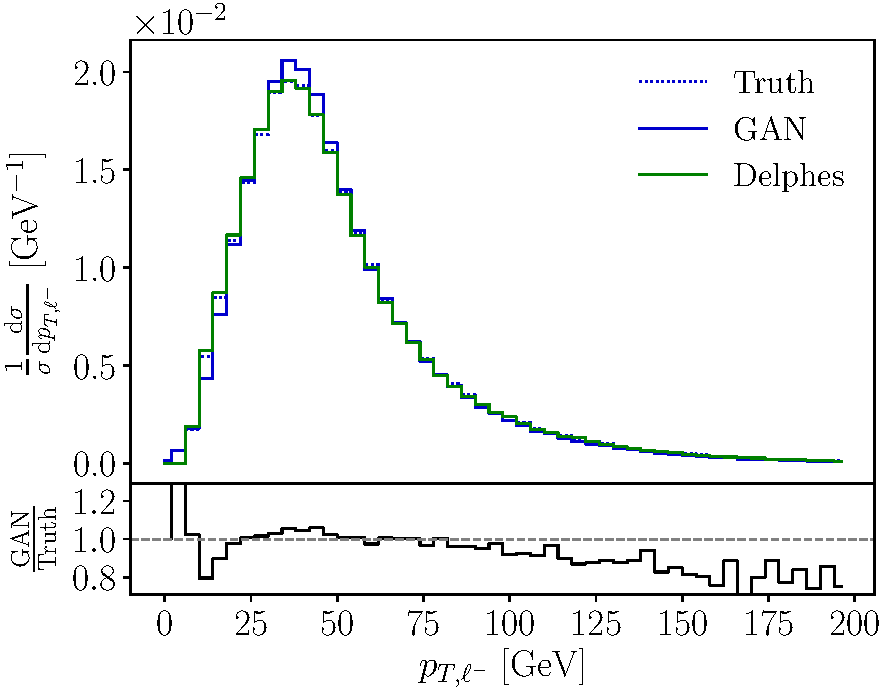
\includegraphics[page = 1, width=0.49\textwidth]{figures/cGAN/GAN_ratio}
\includegraphics[page = 4, width=0.49\textwidth]{figures/cGAN/GAN_ratio}
\caption{Example distributions for parton level truth, after
  detector simulation, and GANned back to parton level. The lower
  panels give the ratio of parton level truth and
  reconstructed parton level.}
\label{fig:distributions_GAN}
\end{figure}
%------------------------------------------------------------

For all GAN trainings we use a dataset of 300k events and assign each
While the smearing of the lepton momenta is modest, 
the observed widths of the hadronically decaying $W$-boson will 
be much larger than the parton-level Breit-Wigner distribution. 
For this reason, we focus on showing hadronic observables to benchmark 
the performance of our set-up.

In Fig.~\ref{fig:distributions_GAN} we
compare true parton-level events to the GAN's output.  
We run the GAN on a set of statistically independent, 
but simulation-wise identical sets of detector-level events. 
Both, the relatively flat $p_{T,j_1}$ and the
peaked $m_{jj}$ distributions agree well between the true parton-level
events and the GAN-inverted sample, indicating that the model
is able to reproduce the parton level observables correctly.

This first approach only serves as a check that the training procedure of the
GAN leads to the correct outcome, as it suffers from severe limitations. 
First of all, we wish to invert the detector simulation stochastically, i.e. 
we want the full posterior distribution of possible parton level events
associated to a single detector level event. As this setting doesn't accommodate
any random input, and the generator itself is a deterministic map, this is 
not possible.
Secondly, the detector information is completely ignored by the model, 
as in the training batches of parton and detector get shuffled independently, 
and there's therefore no connection between each them. 
In order to illustrate this second point better, we invert an event sample which is not
statistically equivalent to the training data, specifically by testing the GAN on 
data covering only part of the detector-level phase space. 
We apply the two sets of jet cuts
%
\begin{alignat}{5}\tag{7}
&\text{Cut I}: & \quad
p_{T,j_1} &= 30~...~100~\gev
\label{eq:jetcut1a} \\\tag{8}
&\text{Cut II}: & \quad
p_{T,j_1} &= 30~...~60~\gev \quad \text{and} \quad p_{T,j_2} = 30~...~50~\gev \; ,
\label{eq:jetcut1b}
\end{alignat}
%
which leave us with 88\% and 38\% of events, respectively. This
approach ensures that the training has access to the full information,
while the test sample is a significantly reduced sub-set of the full
sample.

%------------------------------------------------------------
\begin{figure}[t]
\centering
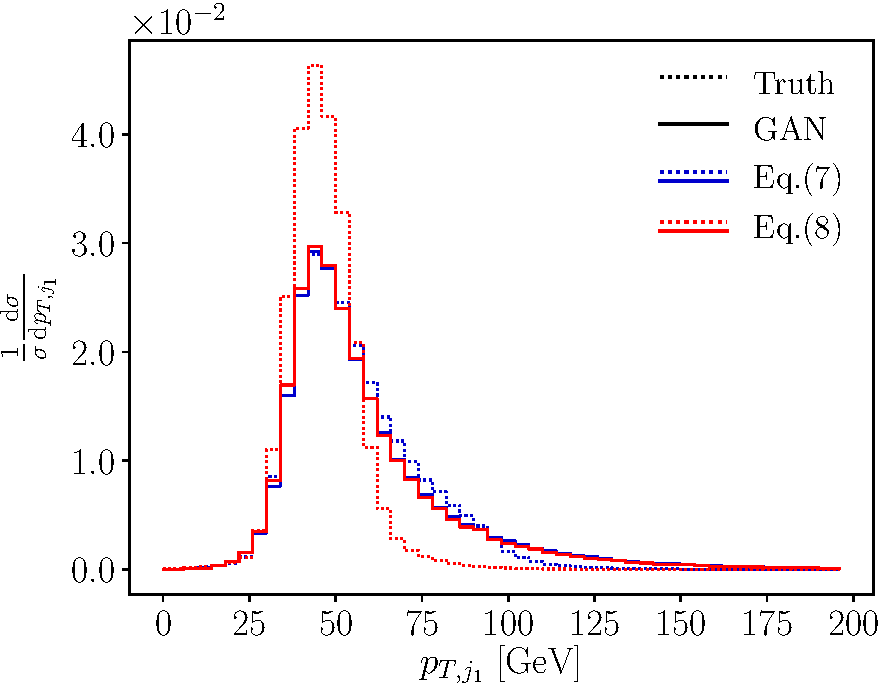
\includegraphics[page = 1, width=0.49\textwidth]{figures/cGAN/GAN_overlap}
\includegraphics[page = 2, width=0.49\textwidth]{figures/cGAN/GAN_overlap}
\caption{Parton level truth and GANned distributions when we train the
  GAN on the full data set but only unfold parts of phase space
  defined in Eq.\eqref{eq:jetcut1a} and Eq.\eqref{eq:jetcut1b}.}
\label{fig:distributions_GAN_sliced}
\end{figure}
%------------------------------------------------------------

In Fig.~\ref{fig:distributions_GAN_sliced} we show a set of kinematic
distributions with detector cuts propagated to the parton level. As
before, we compare the original parton-level shapes of the
distributions with the results from inverting the fast detector
simulation.  
We see that while there's a strong correlation in the paired dataset
used for the training, the model is completely insensitive to it, and 
simply reproduces the full parton level information.
This is clear indications that the naive GAN approach doesn't exploit 
the fact that parton and detector events are paired. We discuss a 
solution in the next section.

%%%%%%%%%%%%%%%%%%%%%%%%%%%%%%%%%%%%%%%%%%%%%%%%%%%%%%%%%
\subsection{Conditional GAN}
\label{sec:fcgan}

%------------------------------------------------------------
\begin{figure}[t]
\centering
%\definecolor{Gcolor}{HTML}{3b528b}
%\definecolor{Dcolor}{HTML}{e41a1c}

\definecolor{Gcolor}{HTML}{2c7fb8}
\definecolor{Dcolor}{HTML}{f03b20}

\tikzstyle{generator} = [thick, rectangle, rounded corners, minimum width=1.5cm, minimum height=1cm,text centered, draw=Gcolor]
\tikzstyle{discriminator} = [thick, rectangle, rounded corners, minimum width=1.5cm, minimum height=1cm,text centered, draw=Dcolor]
\tikzstyle{mmd} = [thick, rectangle, rounded corners, minimum width=1.5cm, minimum height=1cm,text centered, draw=black]
\tikzstyle{io} = [thick,circle, trapezium left angle=70, trapezium right angle=110, minimum width=1.2cm, minimum height=1cm, text centered, draw=black]

\tikzstyle{cond} = [thick, rectangle, dotted, rounded corners, minimum width=10.0cm, minimum height=2cm,text centered, draw=gray!50!black]

\tikzstyle{iodotted} = [thick, circle, trapezium left angle=70, trapezium right angle=110, minimum width=1.2cm, minimum height=1cm, text centered, draw=black, dotted]

\tikzstyle{process} = [thick, rectangle, minimum width=1cm, minimum height=1cm, text centered, draw=black]

\tikzstyle{xG} = [thick,rectangle, minimum width=2.2cm, minimum height=3cm, text depth= 2.2cm, draw=black]
\tikzstyle{s0} = [thick,rectangle, minimum width=2cm, minimum height=3cm, text centered]
\tikzstyle{s1} = [thick, dotted, rectangle, minimum width=1.6cm, minimum height=1.1cm, text centered, draw=black]


\tikzstyle{decision} = [thick,rectangle, minimum width=1cm, minimum height=1cm, text centered, draw=black]


\tikzstyle{dots} = [circle, minimum size=2pt, inner sep=0pt,outer sep=0pt, draw=Dcolor, fill = Dcolor]

\tikzstyle{arrow} = [thick,->,>=stealth]

\begin{tikzpicture}[node distance=2cm]


\node (generator) [generator] {$G$};
\node (random) [io, left of=generator, xshift=-0.2cm, yshift=0cm] {$\{ r \}$};
\draw [arrow, color=black] (random) -- (generator);
\node (xG) [io, right of = generator, xshift=1.0cm, yshift=0cm] {$\{x_G\}$};
\node (discriminator) [discriminator, right of = xG, xshift=1.0cm, yshift=0cm] {$D$};

\node (cond) [cond, above of = generator, xshift=1.5cm, yshift=0.5cm] {};
\node (condi) [above of = xG, xshift=1.9cm, yshift=1.2cm, color=gray!50!black] {Condition};

\node (xd) [io, above of = generator, xshift=0.cm, yshift=0.5cm] {$\{x_d\}$};
\node (xp) [io, below of = xG, xshift=0.5cm, yshift=0cm] {$\{x_p\}$};

\node (detector) [process, left of=xd, xshift=-0.2cm, yshift=0cm] {detector};
\node (parton) [process, left of=xp, xshift=-0.2cm, yshift=0cm] {parton};

\coordinate[ above of= discriminator, xshift=-0.1cm, yshift=0.5cm] (in1);
\draw [thick, color=black] (xd) -- (in1);
\draw [arrow, color=black] (in1) -- ([xshift=-0.1cm] discriminator.north);

\draw [arrow, color=black] (detector) -- (xd);
\draw [arrow, color=black] (parton) -- (xp);
\draw [arrow, color=black] (xd) -- (generator);
\draw [arrow, color=black] (xp) -- (discriminator);
\draw [arrow, color=Gcolor] (generator) -- (xG);
\draw [arrow, color=Gcolor] (xG) -- (discriminator);

\node (dloss) [process, right of=discriminator, xshift=0.5cm, yshift=0cm] {$L_{D}$};
\node (gloss) [process, below of=dloss, xshift=0.0cm, yshift=0cm] {$L_{G}$};
\node (mmd) [mmd, below of=discriminator, xshift=0.0cm, yshift=0cm] {MMD};

\draw [arrow, color=Gcolor] (discriminator) -- (gloss);
\draw [arrow, color=Dcolor] (discriminator) -- (dloss);

\coordinate[ above of = dloss, xshift=0cm, yshift=-1cm] (d1);
\coordinate[ above of = discriminator, xshift=0.1cm, yshift=-1cm] (d2);
\draw[thick, dashed, color=Dcolor] (dloss) -- (d1);
\draw[thick, dashed, color=Dcolor] (d1) -- (d2);
\draw[arrow, dashed, color=Dcolor] (d2) -- ([xshift=0.1cm] discriminator.north);

\draw[arrow, color=Gcolor] (xG) --  (mmd);
\draw[arrow, color=black] (xp) --  (mmd);
\draw[arrow, color=Gcolor] (mmd) --  (gloss);
%\draw[arrow, color=Gcolor] (xd) -- (mmd);


\coordinate[ below of = gloss, xshift=0cm, yshift=1.0cm] (out1);
\coordinate[ below of = generator, xshift=0cm, yshift=-1.0cm] (out2);
\draw[thick, dashed, color=Gcolor] (gloss) --  (out1);
\draw[thick, dashed, color=Gcolor] (out1) --  (out2);
\draw[arrow, dashed, color=Gcolor] (out2) --  (generator);








\end{tikzpicture}

\caption{Structure of our fully conditional FCGAN. The
  input $\{r\}$ describes a batch of random numbers and $\{ x_{G,d,p}
  \}$ denotes events sampled from the generator, detector-level data,
  or parton-level data. The blue (red) arrows indicate which
  connections are used in the training of the generator
  (discriminator).}
\label{fig:FCGAN}
\end{figure}
%------------------------------------------------------------

The issues highlighted in the previous section can be simultaneously solved
by switching to a conditional GAN set-up~\cite{cond_gan}, which we show
 in Fig.~\ref{fig:GANs}. First of all, we recover the physical intuition that
this entire mapping is statistical in nature by feeding the generator random
numbers $\{z\}$ sampled from a simple, fixed distribution, in our case a multivariate
Gaussian with zero mean and the identity as the covariance matrix. The input
is taken with the same dimensionality as the target space.
Secondly, the detector-level information $\{ x_d \}$ is used as an event-by-event conditional input
on the link between a set of random numbers and the parton-level
output, \ie $G( \{ r \}, \{ x_d \} ) = \{ x_G \}$. This way the conditional model
can generate parton-level events from random noise but still using the
detector-level information as input. 
%
%
%The idea behind the conditional set-up is not to learn a deterministic link between input
%and output samples, because we know that without an enforced structure
%in the weight or function space the generator does not benefit from
%the structured input. In other words, the network does not properly
%exploit the fact that the detector-level and parton-level data sets in
%the training sample are paired.  A second, related problem of the
%naive GAN is that once trained the model is completely deterministic,
%so each detector-level event will always be mapped to the same
%parton-level events. This goes against the physical intuition that
%this entire mapping is statistical in nature.

%------------------------------------------------------------

\begin{figure}[t]
\centering
\includegraphics[page = 2, width=0.49\textwidth]{figures/cGAN/cGAN_full_ratio}
\includegraphics[page = 3, width=0.49\textwidth]{figures/cGAN/cGAN_full_ratio} \\
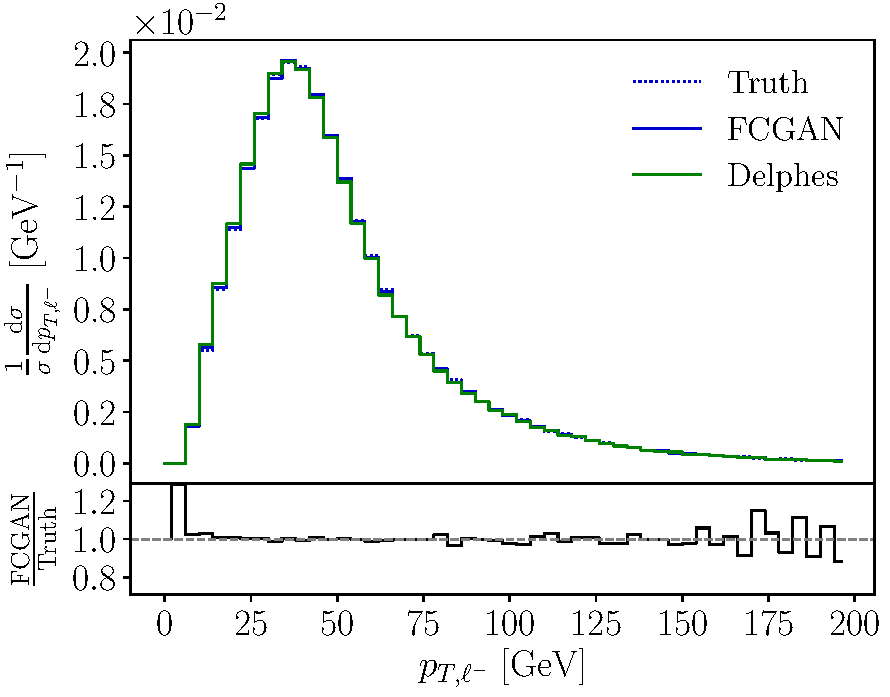
\includegraphics[page = 1, width=0.49\textwidth]{figures/cGAN/cGAN_full_ratio}
\includegraphics[page = 4, width=0.49\textwidth]{figures/cGAN/cGAN_full_ratio}
\caption{Example distributions for parton level truth, after detector
  simulation, and FCGANned back to parton level. The lower panels give
  the ratio of parton level truth and reconstructed parton level.  The
  lower panels give the deviation between parton level truth and
  reconstructed parton level. To be compared with the naive GAN
  results in Fig.~\ref{fig:distributions_GAN}.}
\label{fig:distributions_FCGAN}
\end{figure}
%------------------------------------------------------------

%------------------------------------------------------------
\begin{table}[b!]
\begin{small} \begin{center}
\begin{tabular}{l r | l r}
\toprule
Parameter              & Value   & Parameter              & Value  \\
\midrule
Layers & 12 & Batch size & 512 \\
Units per layer & 512 & Epochs & 1200\\
Trainable weights G & 3M  & Iterations per epoch & 500\\
Trainable weights D & 3M  & Number of training events & $3 \times 10^5$\\
\midrule
$\lambda_G$ & 1 \\
$\lambda_D$ & $10^{-3}$ \\
\bottomrule
\end{tabular}
\end{center} \end{small}
\caption{FCGAN setup.}
\label{tab:details}
\end{table}
%------------------------------------------------------------

In Fig.~\ref{fig:FCGAN} we introduce a fully conditional GAN
(FCGAN).
While the training procedure is identical, we need to modify the objective function as
%
\begin{align}
L_D \to L_D^\text{(FC)}= \left\langle - \log D\left(x, y\right) \right\rangle_{x \sim P_p, y \sim P_d} + \left\langle - \log\left( 1-D\left(x,y\right)\right) \right\rangle_{x \sim P_G, y \sim P_d} \; ,
\label{eq:D_closs}
\end{align}
%
and the regularized loss function changes accordingly,
%
\begin{align}
\begin{split}
L_D^\text{(reg)} \to L_D^\text{(reg,\,FC)} =
L_D^\text{(FC)}
&+ \lambda_D\,
\Langle \left(1- D(x,y)\right)^2 \vert \nabla \phi \vert^2 \Rangle_{x \sim P_p, y \sim P_d} \\
&+ \lambda_D\,
\Langle D\left(x,y\right)^2\, \vert \nabla \phi \vert^2 \Rangle_{x \sim P_G, y \sim P_d}  \; ,
\end{split}
\label{eq:Dcloss2}
\end{align}
%

again using the conventions of Ref.~\cite{gan_phasespace}. The
generator loss function now takes the form
%
\begin{align}
L_G\to L_G^\text{(FC)} = \left\langle - \log D\left(x,y\right) \right\rangle_{x \sim P_G, y \sim P_d} \; .
\label{eq:G_closs}
\end{align}
%
Note, that we do not build a conditional version of the MMD loss.  The
hyper-parameters of our FCGAN are summarized in
Tab.~\ref{tab:details}. Changing from a naive GAN to a
conditional GAN we have to pay a price in the structure of the
training sample. While the naive GAN only required event batches to be
matched between parton level and detector level, the training of the
FCGAN actually requires event-by-event matching.\medskip

In Fig.~\ref{fig:distributions_FCGAN} we compare the truth and the
generated events, trained on and applied to events covering the full
phase space. Compared to the naive GAN, inverting the detector effects
now works even better. The under-estimate of the GAN rate in tails no longer 
occurs for the FCGAN.  The reconstructed invariant
$W$-mass forces the network to dynamically generate a very narrow
physical width from a comparably broad Gaussian peak. Using our usual
MMD loss developed in Ref.~\cite{gan_phasespace} we reproduce the peak
position, width, and peak shape to about 90\%. We emphasize that
the MMD loss requires us to specify the relevant one-dimensional
distribution, in this case $m_{jj}$, but it then extracts the on-shell
mass or width dynamically. The multi-kernel approach we use in this
case is explained in the Appendix.

%------------------------------------------------------------
\begin{figure}[t]
\centering
\includegraphics[page = 2, width=0.49\textwidth]{figures/cGAN/cGAN_overlap_1}
\includegraphics[page = 3, width=0.49\textwidth]{figures/cGAN/cGAN_overlap_1} \\
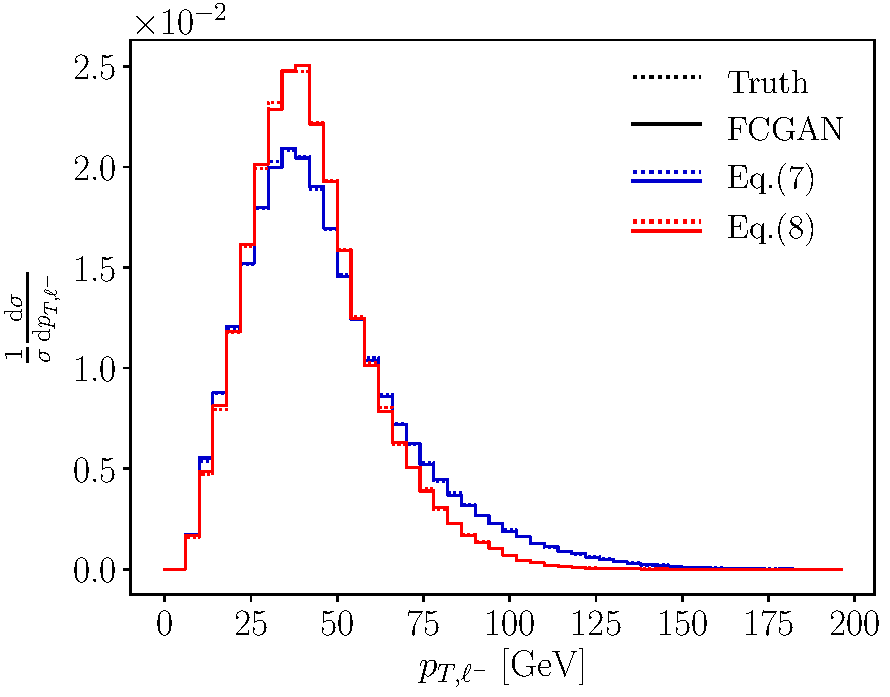
\includegraphics[page = 1, width=0.49\textwidth]{figures/cGAN/cGAN_overlap_1}
\includegraphics[page = 4, width=0.49\textwidth]{figures/cGAN/cGAN_overlap_1}
\caption{Parton level truth and FCGANned distributions when we train
  the GAN on the full data set but only unfold parts of phase space
  defined in Eq.\eqref{eq:jetcut1a} and Eq.\eqref{eq:jetcut1b}. To be
  compared with the naive GAN results in
  Fig.\ref{fig:distributions_GAN_sliced}.}
\label{fig:distributions_FCGAN_sliced_1}
\end{figure}
%------------------------------------------------------------

As for our naive ansatz we now test what happens to the network when
the training data and the test data do not cover the same phase space
region. We train using the entire phase space, but we then only
invert to the 88\% and 38\% of events passing the jet
cuts~I and~II defined in Eq.\eqref{eq:jetcut1a} and
Eq.\eqref{eq:jetcut1b}. We show the results in
Fig.~\ref{fig:distributions_FCGAN_sliced_1}. As observed before,
especially the jet cuts with only 40\% survival probability shape our
four example distributions. However, we see for example in the
$p_{T,jj}$ distribution that the inverted detector-level sample
reconstructs the patterns of the true parton-level events
perfectly. This comparison indicates that the FCGAN approach deals
with differences in the training and test samples very well.

%------------------------------------------------------------
\begin{figure}[t]
\centering
\includegraphics[page = 2, width=0.49\textwidth]{figures/cGAN/cGAN_overlap_2}
\includegraphics[page = 3, width=0.49\textwidth]{figures/cGAN/cGAN_overlap_2} \\
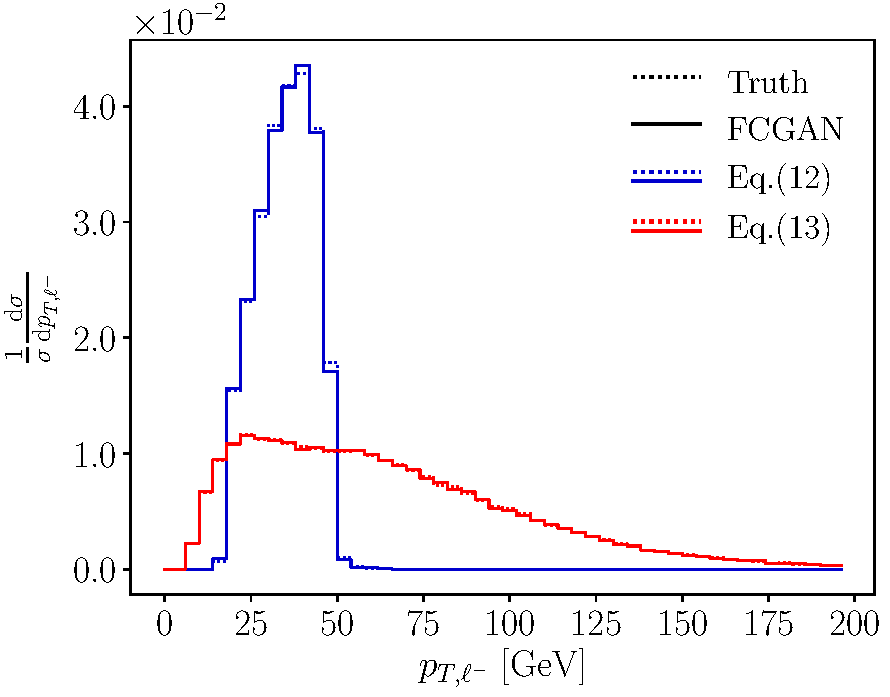
\includegraphics[page = 1, width=0.49\textwidth]{figures/cGAN/cGAN_overlap_2}
\includegraphics[page = 4, width=0.49\textwidth]{figures/cGAN/cGAN_overlap_2}
\caption{Parton level truth and FCGANned distributions when we train
  the GAN on the full data set but only unfold parts of phase space
  defined in Eqs.\eqref{eq:jetcut2a} and~\eqref{eq:jetcut2b}.}
\label{fig:distributions_FCGAN_sliced_2}
\end{figure}
%------------------------------------------------------------

In order to test to which degree the inversion holds, we move on to harsher 
cuts on the inclusive event sample. We start with
%
\begin{align}\tag{12}
\text{Cut III}: \quad p_{T,j_1}= 30~...~50~\gev
\quad p_{T,j_2} = 30~...~40~\gev
\quad p_{T,\ell^-} = 20~...~50~\gev \; ,
\label{eq:jetcut2a}
\end{align}
%
which $14\%$ of all events pass. In
Fig.~\ref{fig:distributions_FCGAN_sliced_2} we see that also for this
much reduced fraction of test events corresponding to the training
sample the FCGAN inversion reproduces the true distributions extremely
well, to a level where it appears not really relevant what fraction of
the training and test data correspond to each other.

Finally, we apply a cut which not only removes a large fraction of
events, but also cuts into the leading peak feature of the $p_{T,j_1}$
distribution and removes one of the side bands needed for an
interpolation,
%
\begin{align}\tag{13}
\text{Cut IV}: \quad  p_{T,j_1} > 60~\gev \; .
\label{eq:jetcut2b}
\end{align}
%
For this choice 39\% of all events pass, but we remove all events at
low transverse momentum, as can be seen from
Fig.~\ref{fig:distributions_FCGAN}. This kind of cut could therefore
be expected to break the unfolding. Indeed, the red lines in
Fig.~\ref{fig:distributions_FCGAN_sliced_2} indicate that we have
broken the $m_{jj}$ reconstruction through the FCGAN. However, all
other (shown) distributions still agree with the parton-level truth
extremely well. The problem with the invariant mass distribution is
that our implementation of the MMD loss is not actually
conditional. At this stage it means that, when pushed
towards its limits, the network will first fail to reproduce the
correct peak width in the $m_{jj}$ distribution, while all other
kinematic variables remain stable.\medskip

%------------------------------------------------------------
\begin{figure}[t]
\centering
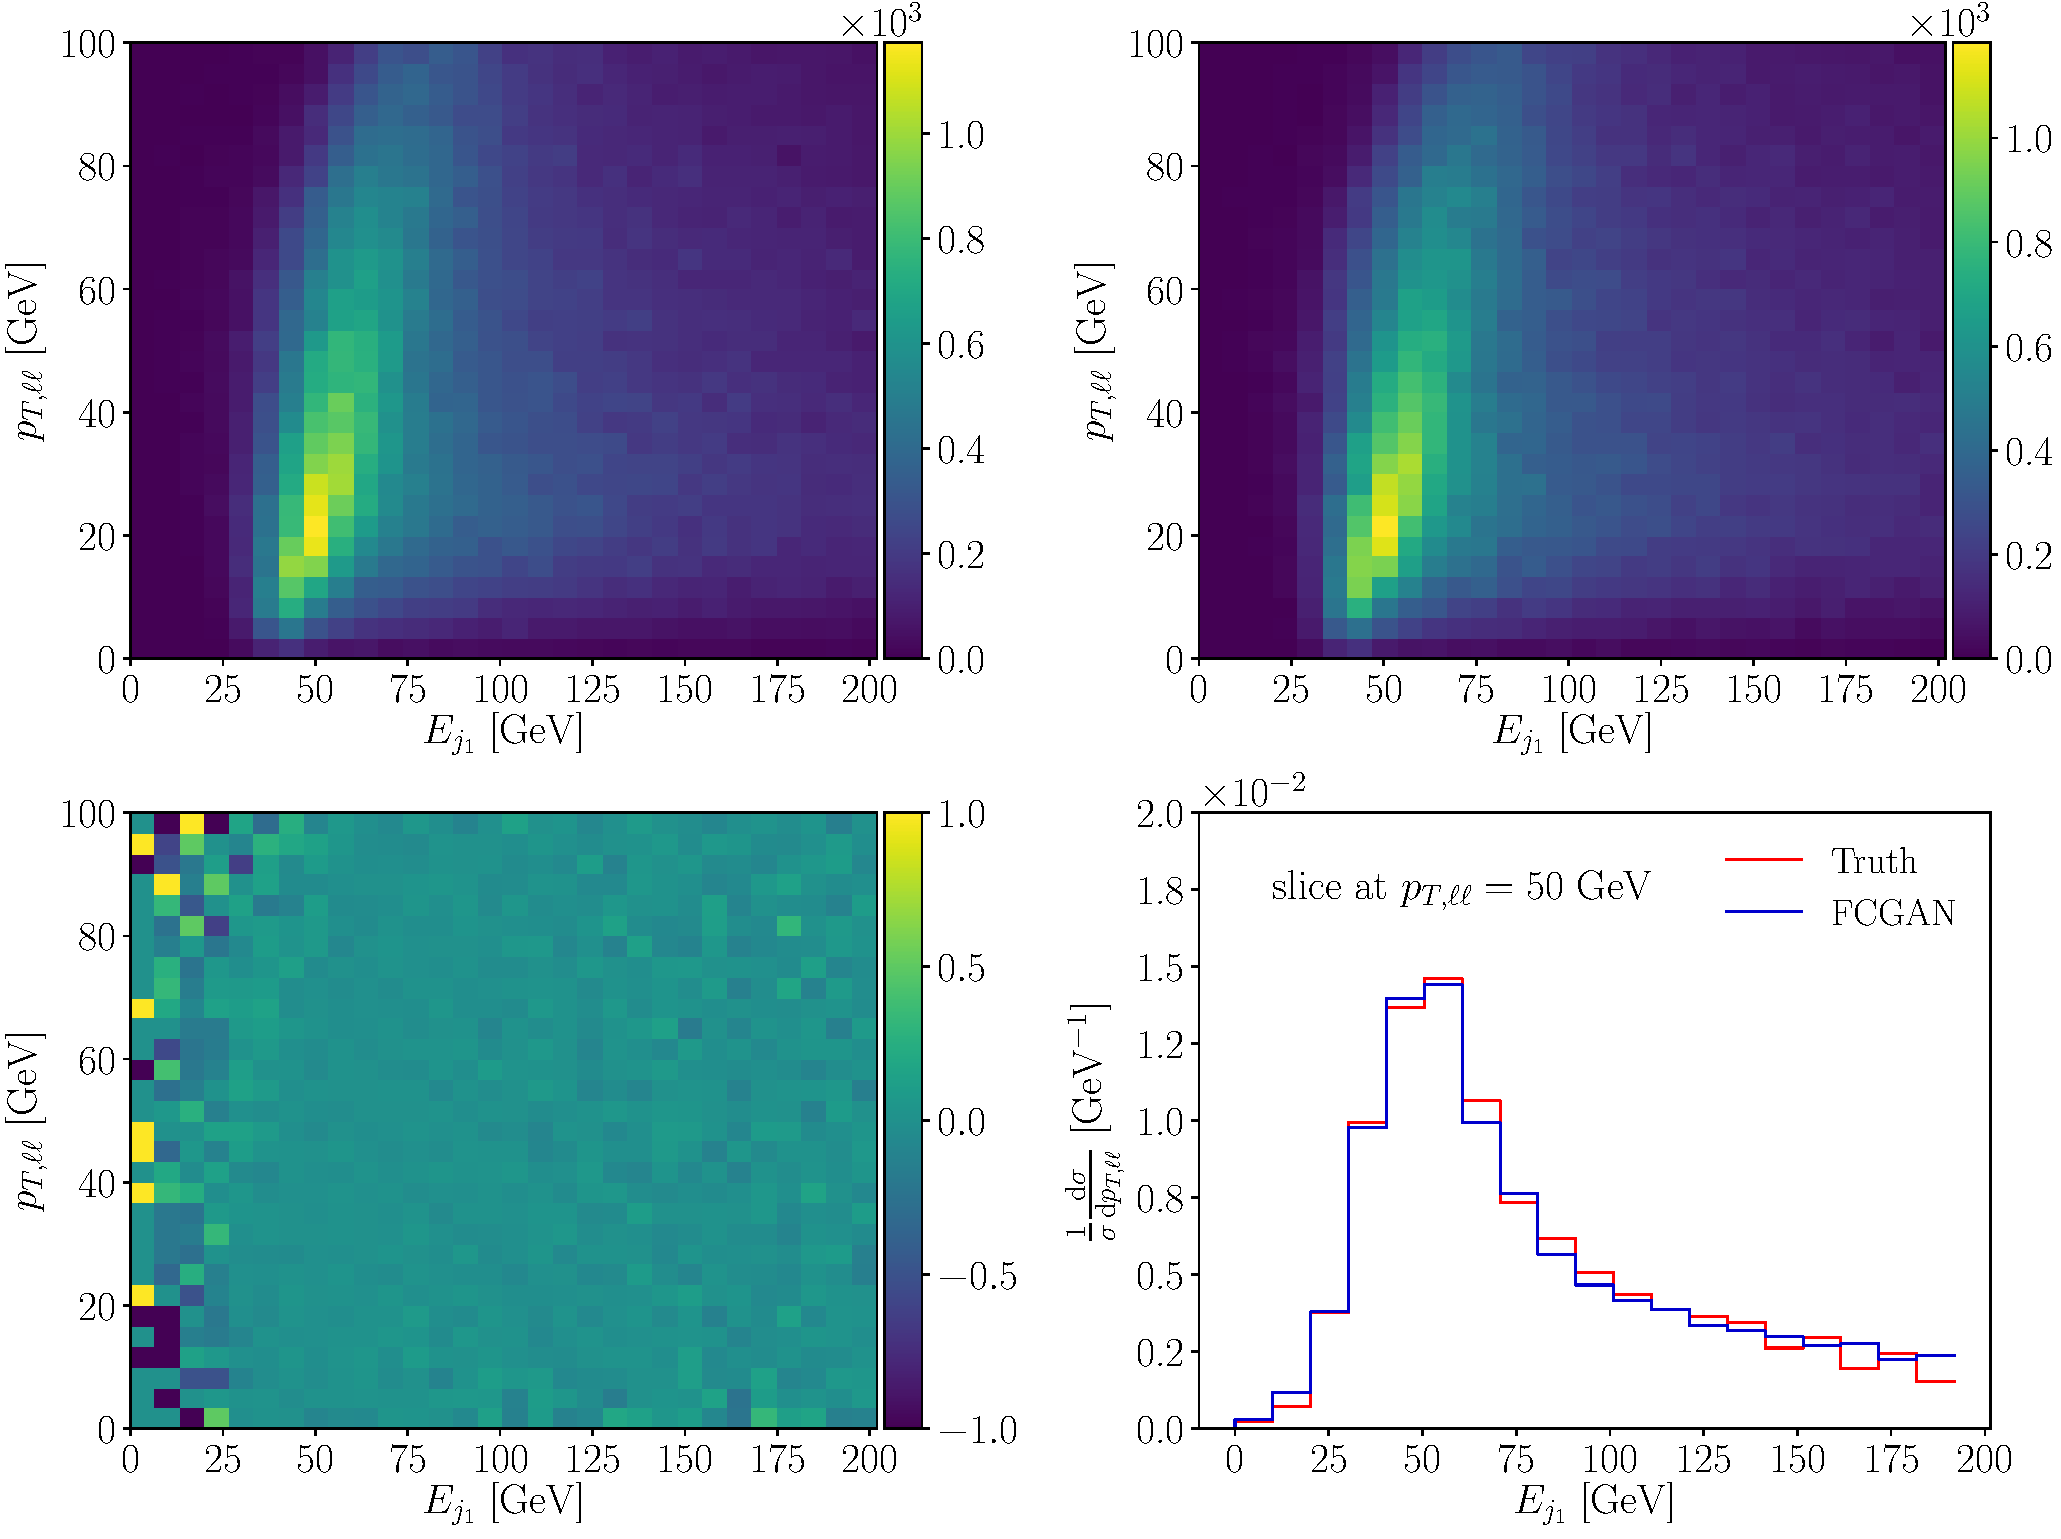
\includegraphics[width=0.98\textwidth]{figures/cGAN/cGAN_2d_corr}
\caption{Two-dimensional parton level truth (upper left) and FCGANned
  (upper right) distributions when we train the GAN on the full data
  set and unfold over the full phase space. The lower panels show the
  relative deviation between truth and FCGANned and the one-dimensional
  $E_{j_1}$ distribution along fixed $p_{T,\ell \ell}$.}
\label{fig:full_2d}
\end{figure}
%------------------------------------------------------------

Finally, just like in Ref.~\cite{gan_phasespace} we show 2-dimensional
correlations in Fig.~\ref{fig:full_2d}. We stick to applying the
network to the full phase space and show the parton level truth and
the FCGAN-inverted events in the two upper panels. Again, we see that
the FCGAN reproduces all features of the parton level truth with high
precision. The bin-wise relative deviation between the two 2-dimensional
distributions only becomes large for small values of $E_{j_1}$, where
the number of training events is extremely small.

%%%%%%%%%%%%%%%%%%%%%%%%%%%%%%%%%%%%%%%%%%%%%%%%%%%%%%%%%
\subsection{New physics injection}
\label{sec:closure}

As discussed before, unfolding to a hard process is necessarily
model-dependent. Until now, we have always assumed the Standard Model
to correctly describe the parton-level and detector-level events. 
An obvious question is what happens if we train our FCGAN on Standard
Model data, but apply it to a different hypothesis. This challenge
becomes especially interesting if this alternative hypothesis differs
from the Standard Model in a local phase space effect. It then allows
us to test if the generator networks maps the parton-level and
detector-level phase spaces in a structured manner. Such features of
neural networks are at the heart of all variational constructions, for
instance variational autoencoders which are structurally close to
GANs. 

To this end we add a fraction of resonant $W'$ events from a
triplet extension of the Standard Model~\cite{Biekoetter:2014jwa},
representing the hard process
%
\begin{align}
p p
\to {W'}^*
\to Z W^\pm
\to (\ell^- \ell^+) \; (j j )
\end{align}
%
to the test data.  We simulate these events with madgraph using the
model implementation of Ref.~\cite{Brehmer:2015rna} and denote the new
massive charged vector boson with a mass of 1.3~TeV and a width of
15~GeV as $W'$. For the test sample we combine the usual Standard
Model sample with the $W'$-sample in proportions $90\% - 10\%$.  The
other new particles do not appear in our process to leading order.
Because we want to test how well the GAN maps local phase space
structures onto each other, we deliberately choose a small width
$\Gamma_{W'}/M_{W'}\sim 1\%$, not exactly typical for such strongly
interacting triplet extensions.

%------------------------------------------------------------
\begin{figure}[t]
\centering
\includegraphics[page = 9, width=0.49\textwidth]{figures/cGAN/6f_plots_mix}
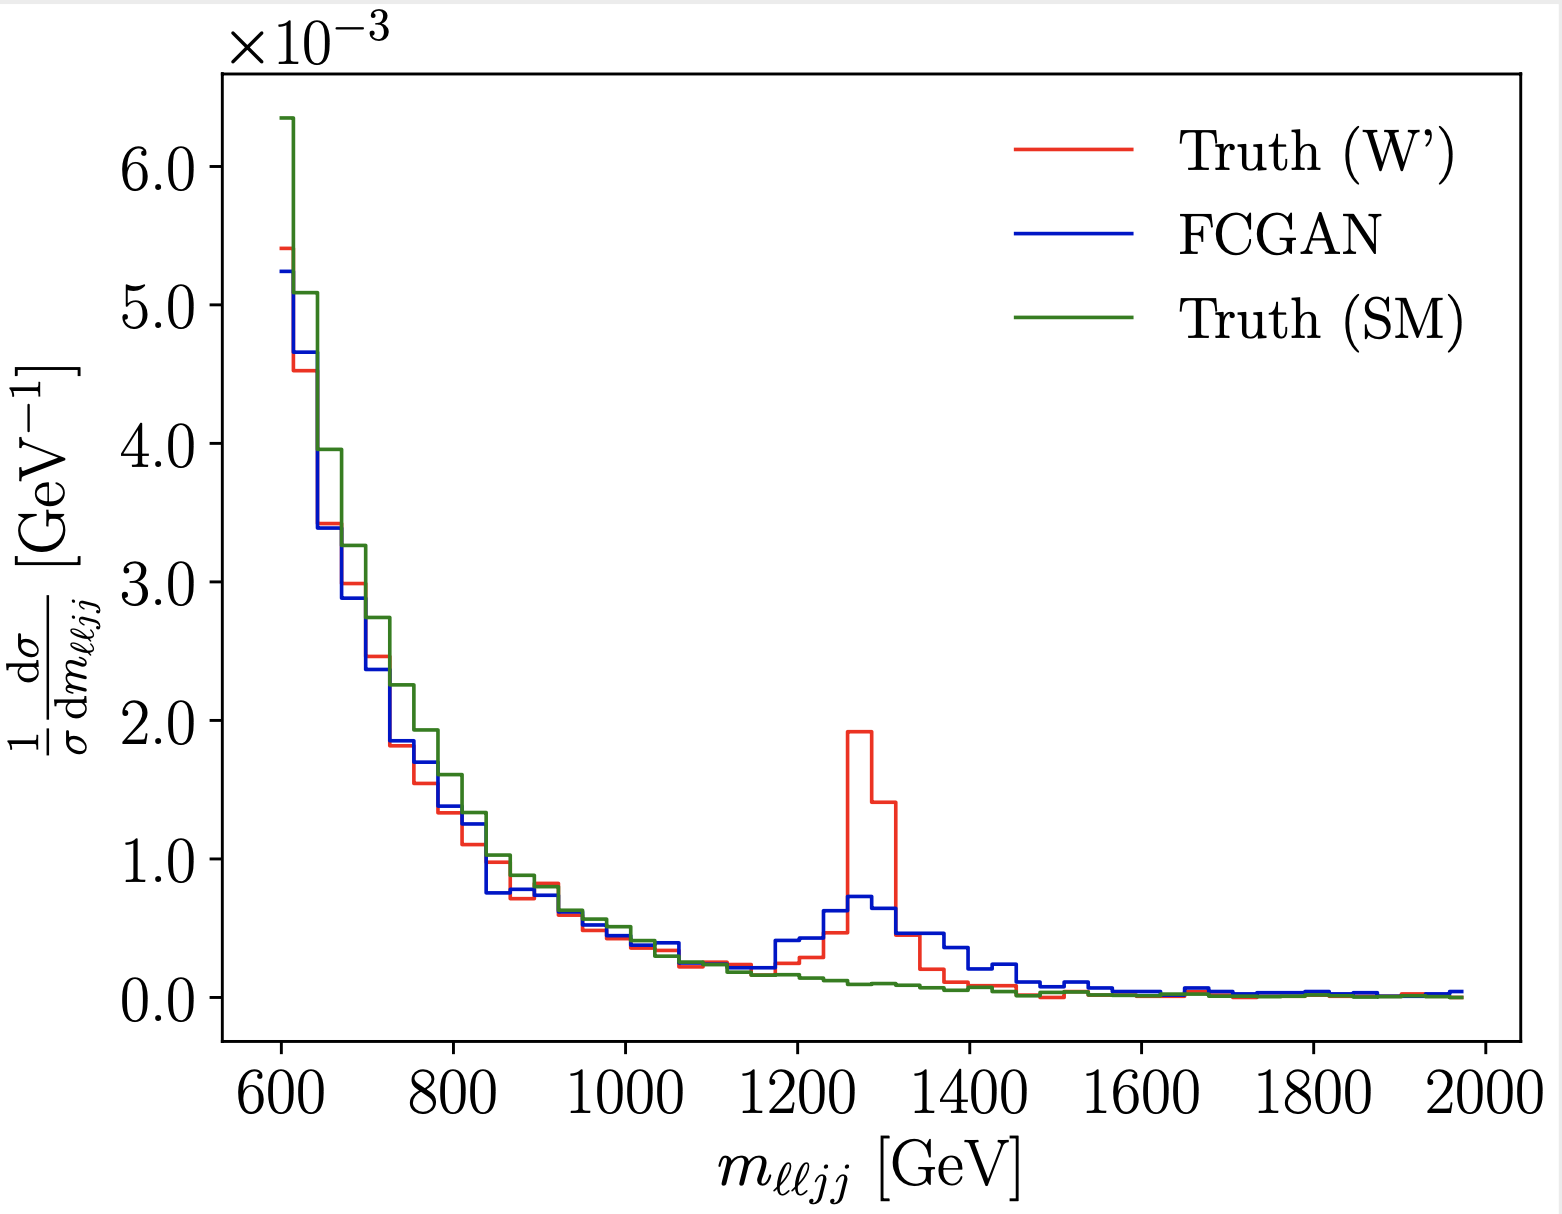
\includegraphics[page = 1, width=0.49\textwidth]{figures/cGAN/6f_plots_mix}\\
\includegraphics[page = 17, width=0.49\textwidth]{figures/cGAN/6f_plots_mix}
\includegraphics[page = 18, width=0.49\textwidth]{figures/cGAN/6f_plots_mix}
\caption{Parton level truth and FCGANned distributions when we train
  the network on the Standard Model only and unfold events with an
  injection of $10\%$ $W'$ events. The mass of the
  additional $s$-channel resonance is 1.3~TeV.}
\label{fig:w_prime}
\end{figure}
%------------------------------------------------------------

The results for this test are shown in Fig.~\ref{fig:w_prime}. First,
we look at transverse momentum distribution of final-state particles,
which are hardly affected by the new heavy resonance. Both, the
leading jet and the lepton distributions are essentially identical for
both truth levels and the FCGAN output. The same is true for the
invariant mass of the hadronically decaying $W$-boson, which
nevertheless provides a useful test of the stability of our training
and testing.

Finally, we show the reconstructed $W'$-mass in the lower-right
pane. Here we see the different (normalized) truth-level distributions
for the Standard Model and the $W'$-injected sample. The FCGAN,
trained on the Standard Model, keeps track of local phase space
structures and reproduces the $W'$ peak faithfully. It also learn the
$W'$-mass as the central peak position very well. The only issue is
the $W'$-width, which the network over-estimates. However, we know
already that dynamically generated width distributions are a challenge
to GANs and require for instance an MMD loss.  Nevertheless,
Fig.~\ref{fig:w_prime} clearly shows that GAN unfolding shows a high
degree of model independence, making use of local structures in the
mapping between the two phase spaces. We emphasize that the additional
mass peak in the FCGANned events is not a one-dimensional feature, but
a localized structure in the full phase space. This local structure is
a feature of neural networks which comes in addition to the known
strengths in interpolation.

%%%%%%%%%%%%%%%%%%%%%%%%%%%%%%%%%%%%%%%%%%%%%%%%%%%%%%%%%

\section{INN unfolding}
\label{sec:inn}

In Sec.~\ref{sec:ganunfolding} we have introduced and developed the idea
of inverting Monte Carlo simulations using a GAN. However, it should be 
clear from Sec.~\ref{intro:normflow} that an invertible model is a more
natural tool to use, as the task we wish to solve consists precisely of 
inverting a well known forward simulation. We will show in this section how
the intuition built with the conditional GAN provides us with a useful 
guideline.

We introduce the conditional INN in two steps, starting with the
non-conditional, standard set-up. The construction of the INN we use in
our analysis combines two goals~\cite{inn}:
%
\begin{enumerate}
\item the mapping from input to output is invertible and the Jacobians
  for both directions are tractable;
\item both directions can be evaluated efficiently. This second
  property goes beyond some other implementations of normalizing
  flow~\cite{nflow1,nflow_review}.
\end{enumerate}
%
While the final aim is not to actually evaluate our INN in both directions, we will
see that these networks can be extremely useful to invert a stochastic
process like detector smearing.

In Sec.~\ref{sec:inn_cond} we will show how the conditional INN
retains a proper statistical notion of the inversion to parton level
phase space.  This avoids a major weakness of standard unfolding
methods, namely that they only work on large enough event samples
condensed to one-dimensional or two-dimensional kinematic
distributions. This could be a missing transverse energy distribution
in mono-jet searches or the rapidities and transverse momenta in top
pair production. To avoid systematics or biases in the full phase
space coverage required by the matrix element method, the unfolding
needs to construct probability distributions in parton-level phase
space, including small numbers of events in tails of kinematic
distributions.

%%%%%%%%%%%%%%%%%%%%%%%%%%%%%%%%%%%%%%%%%%%%%%%%%%%%%%%%%
\subsection{Naive INN}
\label{sec:inn_base}

%------------------------------------------------------------
\begin{figure}[t]
\centering

%\definecolor{Gcolor}{HTML}{3b528b}
%\definecolor{Dcolor}{HTML}{e41a1c}

\definecolor{Gcolor}{HTML}{2c7fb8}
\definecolor{Dcolor}{HTML}{f03b20}


\tikzstyle{INN} = [thick, rectangle, rounded corners, minimum width=2.5cm, minimum height=3.5cm,text centered, draw=Gcolor]
\tikzstyle{preprocessor} = [thick, rectangle, rounded corners, minimum width=1.5cm, minimum height=1cm,text centered, draw=Dcolor]
\tikzstyle{mmd} = [thick, rectangle, rounded corners, minimum width=1.5cm, minimum height=1cm,text centered, draw=black]
\tikzstyle{io} = [thick,circle, minimum width=1.2cm, minimum height=1.2cm, text centered, draw=black]

\tikzstyle{cond} = [thick, rectangle, dotted, rounded corners, minimum width=10.0cm, minimum height=2cm,text centered, draw=gray!50!black]

\tikzstyle{iodotted} = [thick, circle, minimum width=1.2cm, minimum height=1cm, text centered, draw=black, dotted]

\tikzstyle{process} = [thick, rectangle, minimum width=1cm, minimum height=1cm, text centered, draw=black]

\tikzstyle{xG} = [thick,rectangle, minimum width=2.2cm, minimum height=3cm, text depth= 2.2cm, draw=black]
\tikzstyle{s0} = [thick,rectangle, minimum width=2cm, minimum height=3cm, text centered]
\tikzstyle{s1} = [thick, dotted, rectangle, minimum width=1.6cm, minimum height=1.1cm, text centered, draw=black]


\tikzstyle{decision} = [thick,rectangle, minimum width=1cm, minimum height=1cm, text centered, draw=black]


\tikzstyle{dots} = [circle, minimum size=2pt, inner sep=0pt,outer sep=0pt, draw=Dcolor, fill = Dcolor]

\tikzstyle{arrow} = [thick,->,>=stealth]

\begin{tikzpicture}[node distance=2cm]


\node (INN) [INN] {INN};

\node (xG) [io, left of = INN, xshift=-0.8cm, yshift=1cm] {$\{\tilde x_{p}, \tilde r_{p}\}$};
\node (rG) [io, right of = INN, xshift=0.8cm, yshift=-1cm] {$\{\tilde x_{d}, \tilde r_{d}\}$};


\node (xp) [io, left of = INN, xshift=-0.8cm, yshift=-1cm] {$\{x_p, r_p\}$};
\node (parton) [process, below of=xp, xshift=0cm, yshift=0cm] {parton};
\node (mmd) [mmd, left of=xp, xshift=0.0cm, yshift=1cm] {$L_\text{MMD, MSE}$};

\node (random) [io, right of=INN, xshift=0.8cm, yshift=1cm] {$\{ x_d, r_d \}$};
\node (detector) [process, above of=random, xshift=0cm, yshift=0cm] {detector};
\node (gauss) [mmd, right of=rG, xshift=0.0cm, yshift=1cm] {$L_\text{MMD, MSE}$};


%\node (cond) [cond, above of = xG, xshift=1.5cm, yshift=-0.1cm] {};
%\node (condi) [above of = xG, xshift=1.9cm, yshift=0.5cm, color=gray!50!black] {Condition};

%\node (preprocessor) [preprocessor, above of=INN, xshift=0cm, yshift=0.5cm] {Subnet};
%\node (xd) [io, left of = preprocessor, xshift=-0.5cm, yshift=0cm] {$\{x_d\}$};
%\node (detector) [process, left of=xd, xshift=-0.2cm, yshift=0cm] {detector};

\coordinate[ right of = rG, xshift=0cm, yshift=0cm] (Gin1);
\coordinate[ right of = random, xshift=0cm, yshift=0cm] (Gin2);

\coordinate[ left of = xG, xshift=0cm, yshift=0cm] (MMDin1);
\coordinate[ left of = xp, xshift=0cm, yshift=0cm] (MMDin2);



%\draw [arrow, color=black] ([yshift=0em]random.west) -- ([yshift=1.5em]INN.east);
%\draw [arrow, color=black] ([yshift=-1.5em]INN.east) -- (rG.west);
%\draw [arrow, color=black] ([yshift=1.5em]INN.west) -- (xG.east);
%\draw [arrow, color=black] ([yshift=0em]xp.east) -- ([yshift=-1.5em]INN.west);

\draw [arrow, color=black] ([yshift=0em]parton.north) -- ([yshift=0em]xp.south);
\draw [arrow, color=black] ([yshift=0em]detector.south) -- ([yshift=0em]random.north);

\draw [thick, color=Gcolor] ([yshift=0em]xp.west) -- ([yshift=0em]MMDin2);
\draw [arrow, color=Gcolor] ([yshift=0em]MMDin2) -- ([yshift=0em]mmd.south);
\draw [thick, color=Gcolor] ([yshift=0em]xG.west) -- ([yshift=0em]MMDin1);
\draw [arrow, color=Gcolor] ([yshift=0em]MMDin1) -- ([yshift=0em]mmd.north);

\draw [thick, color=Gcolor] ([yshift=0em]random.east) -- ([yshift=0em]Gin2);
\draw [arrow, color=Gcolor] ([yshift=0em]Gin2) -- ([yshift=0em]gauss.north);
\draw [thick, color=Gcolor] ([yshift=0em]rG.east) -- ([yshift=0em]Gin1);
\draw [arrow, color=Gcolor] ([yshift=0em]Gin1) -- ([yshift=0em]gauss.south);

%\draw [arrow, color=black] ([yshift=0em]detector.east) -- ([yshift=0em]xd.west);
%\draw [arrow, color=black] ([yshift=0em]xd.east) -- ([yshift=0em]preprocessor.west);
%\draw [arrow, color=black] ([yshift=0em]preprocessor.south) -- ([yshift=0em]INN.north);

%\draw[arrow, thick, color=Gcolor] (random.west) -- (xG.east);
\draw[arrow, color=Gcolor] (random.west) --  node[scale=0.8, sloped, anchor=center, above, color=Gcolor]{$\bar{g}(x_d, r_d)$} ([yshift=0cm]xG.east);
%\draw[arrow, thick, color=Gcolor] ([yshift=1cm]INN.west) -- (xG.east);
%\draw[arrow, thick, color=Gcolor] (xp.east) -- (rG.west);
%\draw[arrow, thick, color=Gcolor] (xp.east) -- ([yshift=-1cm]INN.west);
\draw[arrow, color=Gcolor] ([yshift=0cm]xp.east) --  node[scale=0.8, sloped, anchor=center, above, color=Gcolor]{$g(x_p, r_p)$} (rG.west);



\draw[arrow, thick, dashed, color=black] (mmd) -- (INN.west);
\draw[arrow, thick, dashed, color=black] (gauss) -- (INN.east);


\end{tikzpicture}

\caption{Structure of INN. The $\{ x_{d,p} \}$ denote detector-level
  and parton-level events, $\{ r_{d,p} \}$ are random numbers to match
  the phase space dimensionality. A tilde indicates the INN
  generation.}
\label{fig:inn}
\end{figure}
%------------------------------------------------------------

While it is clear from our discussion in Sec.~\ref{sec:ganunfolding} that a
standard INN will not serve our purpose, we still describe it in some
detail before we extend it to a conditional network.  
Following the conventions of our GAN analysis and in analogy to Eqs.\eqref{eq:toy1}
to \eqref{eq:toy3} we define the network input as a vector of hard
process information $x_p \in R^{D_p}$ and the output at detector level
via the vector $x_d \in \mathbb{R}^{D_d}$. 
as the INN is a change of variable, the input and output dimensionalities must be
the same. If the dimensionality of the spaces are such that $D_p < D_d$ 
we can add a noise vector $r$ with dimension
$D_d-D_p$ to define the bijective, invertible transformation,
%
\begin{align}
\begin{pmatrix} x_p \\ r \end{pmatrix}
\stackrel[\leftarrow \; \text{unfolding}: \bar{g}]{\textsc{Pythia,Delphes}: g \rightarrow}{\xleftrightarrow{\hspace*{3.5cm}}}
 x_d  \; .
\label{eq:mapping}
\end{align}
%
A correctly trained network $g$ with the parameters $\theta$
then reproduces $x_d$ from the combination $x_p$ and $r$. Its inverse
$\bar{g}$ instead reproduces the combination of $x_p$ and $r$ from $x_d$.

We have introduced in Sec.~\ref{intro:normflow} the general features of 
invertible models, i.e. models that learn both directions of the bijective mapping in parallel
and encodes them into one network as illustrated in Fig.~\ref{fig:inn} .
In particular, we have explained how we can think of an INN as the composition
of multiple copies of a single base function with the required properties
of invertibility and cheap Jacobian.
For our INN we have chosen invertible coupling layers~\cite{coupling1,coupling2}
based on dimensional partitioning.  For
notational purposes we ignore the random numbers in
Eq.\eqref{eq:mapping} and assume that this layer links an input vector
$x_p$ to an output vector $x_d$ after splitting both of them in
halves, $x_{p,i}$ and $x_{d,i}$ for $i=1,2$. The relation between
input and output is given by a sub-network, which encodes arbitrary
functions $s_{1,2}$ and $t_{1,2}$.  Using an element-wise
multiplication~$\odot$ and sum one could for instance define an output
$x_{d,1}(x_p) = x_{p,1} \odot s_2(x_{p,2}) + t_2(x_{p,2})$. 
In order to avoid numerical instabilities caused by the division with 
$s(x)$ in the inverse direction, we include an exponential to obtain
%
\begin{align}
\begin{pmatrix} x_{d,1} \\ x_{d,2} \end{pmatrix} =
\begin{pmatrix}
x_{p,1} \odot e^{s_2(x_{p,2})} + t_2(x_{p,2}) \\
x_{p,2} \odot e^{s_1(x_{d,1})} + t_1(x_{d,1})
\end{pmatrix}
\hspace{0.5em} \Leftrightarrow \hspace{0.5em}
\begin{pmatrix} x_{p,1} \\ x_{p,2} \end{pmatrix} =
\begin{pmatrix}
(x_{d,1} - t_2(x_{p,2})) \odot e^{-s_2(x_{p,2})} \\
(x_{d,2} - t_1(x_{d,1})) \odot e^{-s_1(x_{d,1})}
\end{pmatrix} \; .
\label{eq:layers}
\end{align}
%
By construction, this inversion works independent of the form of $s$
and $t$. If we write the coupling block function as $g(x_p) \sim x_d$,
again omitting the random numbers $r$, the Jacobian of the network
function has a triangular form
%
\begin{align}
\frac{\partial g(x_p)}{\partial x_p} =
\begin{pmatrix}
\text{diag } e^{s_2(x_{p,2})} & \text{finite} \\
0 & \text{diag } e^{s_1(x_{d,1})}
\end{pmatrix} \; ,
\label{eq:jacob}
\end{align}
%
so its determinant is easy to compute. Such coupling layer
transformations define the normalizing flow, when we view it
as transforming an initial probability density into a very general
form of probability density through a series of invertible steps. We
can relate the two probability densities as long as the Jacobians of
the individual layers can be efficiently calculated.

Since the first use of the invertible coupling layer, much effort has
gone into improving its efficiency. The All-in-One (AIO) coupling
layer includes two features, introduced by Ref.~\cite{coupling2} and
Ref.~\cite{glow}. The first modification replaces the transformation
of $x_{p,2}$ by a permutation of the output of each layer. Due to the
permutation each component still gets modified after passing through
several layers. The second modification includes a global affine transformation
to include a global bias and linear scaling that maps $x \rightarrow s
x + b$. Finally, we apply a bijective soft clamping after the
exponential function in Eq.\eqref{eq:layers} to prevent instabilities
from diverging outputs.

The INN in our simplified example combines three contributions to the
loss function. First, it tests if in the \textsc{Delphes} direction of
Eq.\eqref{eq:mapping} we indeed find $g(x_p) = x_d$ via the mean
squared error (MSE) function. While this is theoretically sufficient
to obtain the inverse function, also testing the inverse direction
$\bar{g}(x_d) = x_p$ greatly improves the efficiency and stability of
the training. Third, to resolve special sharp features like the
invariant mass of intermediate particles we use the MMD loss introduced 
in Sec.~\ref{sec:ganunfolding}. 
%Because we will also use the MMD in another function
%function~\cite{gan_phasespace} we review it briefly. An MMD loss
%allows us to compare any pre-defined distribution. For a relativistic
%phase space a critical narrow phase space feature is the invariant
%mass of intermediate particles. We can force the network to consider
%this one-dimensional distribution of the 4-vectors $x_p$ for batches
%of parton-level and detector-level events,
%%
%\begin{align}
%\text{MMD} =
%\left[ \langle k\left(x,x'\right)\rangle_{x,x' \sim P_p}
%     + \langle k\left(y,y'\right)\rangle_{y,y' \sim P_d}
%     - 2 \langle k\left(x,y \right)\rangle_{x\sim P_p,y \sim P_d} \right]^{1/2} \; .
%\label{eq:MMD2}
%\end{align}
%%
%In Refs.~\cite{gan_phasespace} and~\cite{fcgan} we compare common
%choices, like Gaussian or Breit-Wigner kernels
%%
%\begin{align}
%k_\text{Gauss} \left(x,y\right) = \exp \frac{- \left(x - y\right)^2}{2 \sigma^2}
%\qquad \text{or} \qquad
%k_\text{BW}\left(x,y\right) = \frac{\sigma^2}{\left(x - y\right)^2 + \sigma^2}
%\label{eq:kernels2}
% \end{align}
%%
%with a fixed or variable width $\sigma$~\cite{fcgan}. 
For the INN architecture the Breit-Wigner kernel is the best choice to analyze the
distribution of the random numbers as part of the loss
function~\cite{inn}.

%------------------------------------------------------------
\begin{figure}[t]
%\centering
\includegraphics[page=25, width=0.48\textwidth]{figures/cINN/INN_noE}
\includegraphics[page=25, width=0.48\textwidth]{figures/cINN/INN_FineTune} \\
\includegraphics[page=26, width=0.48\textwidth]{figures/cINN/INN_noE}
\includegraphics[page=26, width=0.48\textwidth]{figures/cINN/INN_FineTune} \\
\includegraphics[page=32, width=0.48\textwidth]{figures/cINN/INN_noE}
\includegraphics[page=32, width=0.48\textwidth]{figures/cINN/INN_FineTune}
\caption{INN-generated $p_{T,q}$ and $M_{W,\text{reco}}$ distributions from a
  naive INN (left) and the noise-extended eINN (right). In green we
  compare the detector-level truth to INNed events transformed from
  parton level. In blue we compare the parton-level truth to INNed
  events transformed from detector level. The secondary panels show
  the ratio of INNed events over parton-level truth. More
  distributions can be found in the pdf files submitted to the arXiv.}
\label{fig:UnfoldCurve}
\end{figure}
%------------------------------------------------------------

We now use the INN network to map parton-level events to
detector-level events or vice-versa. In a statistical analysis we then
use standard kinematic distributions and compare the respective truth
and INN-inverted shapes for both directions. The left panels of
Fig.~\ref{fig:UnfoldCurve} shows the transverse momentum distributions
of the two jets and their invariant mass for both directions of the
INN. The truth events at parton level and at detector level are marked
as dashed lines. Starting from each of the truth events we can apply
the INN describing the detector effects as $x_d = g(x_p)$ or unfolding
the detector effects as $x_p = \bar{g}(x_d)$ in
Eq.\eqref{eq:mapping}. The corresponding solid lines have to be
compared to the dotted truth lines, where we need to keep in mind that
at the parton level the relevant objects are quarks while at the
detector level they are jets.

For the leading jet the truth and INN-generated detector-level agree very
well, while for the second jet the naive INN fails to capture the hard
cut imposed by the jet definition. 
For the invariant mass we find that
the smearing due to the detector effects is reproduced well with some
small deviations in the tails. In the unfolding direction both $p_T$
distributions follow the parton level truth. The only difference is a
systematic lack of events in the tail for the second quark. This is
especially visible in the ratio of the INN-unfolded events and the
parton-level truth, indicating that also at small $p_T$ the network
does not fill the phase space sufficiently. Combining both directions
we see that in forward direction the INN produces a too broad
$p_T$-distribution, the unfolding direction of the INN produces a too
narrow distribution.  The conceptual advantage of the INN actually
implies a disadvantage for the inversion of particular difficult
features.  Finally, the invariant mass of the $W$ is reproduced
perfectly without any systematic deviation.

%%%%%%%%%%%%%%%%%%%%%%%%%%%%%%%%%%%%%%%%%%%%%%%%%%%%%%%%%
\subsection{Noise-extended INN}
\label{sec:inn_noise}

While our simplified example in the previous section shows the potential
 of INNs, it fails to incorporate key aspects of the physical
process.  First of all, the number of degrees of freedom is not
actually the same at parton level and at detector level. External
partons are on their mass shell, while jets come with a range of jet
masses. This mismatch becomes crucial when we include missing
transverse momentum in the signature.  We generally need fewer
parameters to describe the partonic scattering than the detector-level
process.  For a fixed set of parton-level momenta we usually smear
each momentum component to simulate the detector measurement. These
additional degrees of freedom are of stochastic nature, so adding
Gaussian random variable on the parton side of the INN could be a
first step to address this problem.

To also account for potentially unobservable degrees of freedom at the
parton level we extend each side of the INN by a random number vector.
The mapping in Eq.\eqref{eq:mapping} now includes two random number
vectors with dimensions $D_{r_d} = D_p$ and $D_{r_p} = D_d$,
%
\begin{align}
\begin{pmatrix} x_p \\ r_p \end{pmatrix}
\stackrel[\leftarrow \; \text{unfolding}: \bar{g}]{\textsc{Pythia,Delphes}: g \rightarrow}{\xleftrightarrow{\hspace*{3.5cm}}}
\begin{pmatrix} x_d \\ r_d \end{pmatrix} \; .
\label{eq:mappingnoise}
\end{align}
%
In addition, a pure MSE loss can not capture the fact that the
additional noise generates a distribution of detector-level events
given fixed parton momenta. It would just predict a mean value of
this distribution and minimize the effect of the noise. A better
solution is an MMD loss for each degree of freedom in the event and
the masses of intermediate particles, as well as the Gaussian random
variables. On the side of the random numbers this MMD loss ensures
that they really only encode noise. Again it is beneficial for the
training to use the inverse direction and apply additional MMD
losses to the parton level events as well as the corresponding
Gaussian inputs.  Finally we add a weak MSE loss on the four vectors
of each side to stabilize the training.

In the right panels of Fig.~\ref{fig:UnfoldCurve} we show results for
this noise-extended INN (eINN). The generated distributions are similar to
the naive INN case and match the truth at the parton level. A notable
difference appears in the second jet, the weak spot of the naive
INN. The additional random numbers and MMDs provide more freedom to
generate the peak in the forward direction and also improve the
unfolding in the low-$p_T$ and high-$p_T$ regimes.\bigskip

%------------------------------------------------------------
\begin{figure}[t]
\includegraphics[page=9, width=0.48\textwidth]{figures/cINN/point1_inn_fcgan}
\includegraphics[page=20, width=0.48\textwidth]{figures/cINN/CalibrationCurveINNFCGAN}
\caption{Left: illustration of the statistical interpretation of
  unfolded events for one event. Right: calibration curves for
  $p_{T,q_1}$ extracted from the FCGAN and the noise-extended eINN.}
\label{fig:quantile1}
\end{figure}
%------------------------------------------------------------

The noise extension allows for a
statistic interpretation of the generated distributions and a test of
the integrity of the INN-inverted distributions. In the left panel of
Fig.~\ref{fig:quantile1} we illustrate the goal of the statistical
treatment: we start from a single event at the detector level and
generate a set of unfolded events. For each of them we evaluate for
instance $p_{T,q_1}$. Already in this illustration we see that the GAN
output is lacking a statistical behaviour at the level of individual
events, while the noise-extended eINN returns a reasonable
distribution of unfolded events.

To see if the width of this INN output is correct we take 1500
parton-level and detector-level event pairs and unfold each event 60
times, sampling over the random variables. This gives us 1500
combinations like the one shown in the left panel of
Fig.~\ref{fig:quantile1}: a single parton-level truth configuration
and a distribution of the INNed configuration. To see if the central
value and the width of the INNed distribution can be interpreted
statistically as a posterior probability distribution in parton phase
space we analyse where the truth lies within the INN distribution for
each of the 1500 events.  For a correctly calibrated curve we start
for instance from the left of the kinematic distribution and expect
10\% of the 1500 events in the 10\% quantile of the respective
probability distribution, 20\% of events in the 20\% quantile, etc.
The corresponding calibration curves for the noise-extended eINN are
shown in the right panel of Fig.~\ref{fig:quantile1}. While they
indicate that we can attempt a statistical interpretation of the INN
unfolding, the calibration is not (yet) perfect.  A steep rise for the
lower quantile indicates that too many events end up in the first 10\%
quantile. In other words, the distributions we obtain by sampling over
the Gaussian noise for each event are too narrow.

While our noise-extended eINN takes several steps in the right
direction, it still faces major challenges: the combination of many
different loss functions is sensitive to their relative weights; the
balance between MSE and MMD on event constituents has to be calibrated
carefully to generate reasonable quantile distributions; when we want
to extend the INN to include more detector-level information we have
to include an equally large number of random variable on the parton
level which makes the training very inefficient. This leads us
again~\cite{fcgan} to adopt a conditional set-up.

%%%%%%%%%%%%%%%%%%%%%%%%%%%%%%%%%%%%%%%%%%%%%%%%%%%%%%%%%%%%%%%%%%%%%%%%
\subsection{Conditional INN}
\label{sec:inn_cond}

If a distribution of parton-level events can be described by $n$
degrees of freedom, we should be able to use normalizing flows or an
INN to map a $n$-dimensional random number vector onto parton-level
4-momenta.  To capture the information from the detector-level events
we need to condition the INN on these
events~\cite{goodfellow,cond_gan,fcgan}, so we link the parton-level
data $x_p$ to random noise $r$ under the condition of $x_d$. Trained
on a given process the network should now be able to generate
probability distributions for parton-level configurations given a
detector-level event and an unfolding model. We note that the cINN
is still invertible in the sense that it includes a bi-directional
training from Gaussian random numbers to parton-level events and
back. While this bi-directional training does not represent the
inversion of a detector simulation anymore, it does stabilize the
training by requiring the noise to be Gaussian.

%------------------------------------------------------------
\begin{figure}[t]
\centering

%\definecolor{Gcolor}{HTML}{3b528b}
%\definecolor{Dcolor}{HTML}{e41a1c}

\definecolor{Gcolor}{HTML}{2c7fb8}
\definecolor{Dcolor}{HTML}{f03b20}


\tikzstyle{cINN} = [thick, rectangle, rounded corners, minimum width=2.5cm, minimum height=3.5cm,text centered, draw=Gcolor]
\tikzstyle{preprocessor} = [thick, rectangle, rounded corners, minimum width=1.5cm, minimum height=1cm,text centered, draw=Dcolor]
\tikzstyle{mmd} = [thick, rectangle, rounded corners, minimum width=1.5cm, minimum height=1cm,text centered, draw=black]
\tikzstyle{io} = [thick,circle, minimum width=1.2cm, minimum height=1cm, text centered, draw=black]

\tikzstyle{cond} = [thick, rectangle, dotted, rounded corners, minimum width=10.0cm, minimum height=2cm,text centered, draw=gray!50!black]

\tikzstyle{iodotted} = [thick, circle, minimum width=1.2cm, minimum height=1cm, text centered, draw=black, dotted]

\tikzstyle{process} = [thick, rectangle, minimum width=1cm, minimum height=1cm, text centered, draw=black]

\tikzstyle{xG} = [thick,rectangle, minimum width=2.2cm, minimum height=3cm, text depth= 2.2cm, draw=black]
\tikzstyle{s0} = [thick,rectangle, minimum width=2cm, minimum height=3cm, text centered]
\tikzstyle{s1} = [thick, dotted, rectangle, minimum width=1.6cm, minimum height=1.1cm, text centered, draw=black]


\tikzstyle{decision} = [thick,rectangle, minimum width=1cm, minimum height=1cm, text centered, draw=black]


\tikzstyle{dots} = [circle, minimum size=2pt, inner sep=0pt,outer sep=0pt, draw=Dcolor, fill = Dcolor]

\tikzstyle{arrow} = [thick,->,>=stealth]

\begin{tikzpicture}[node distance=2cm]


\node (cINN) [cINN] {cINN};

\node (xG) [io, left of = cINN, xshift=-0.5cm, yshift=1cm] {$\{\tilde{x}_p\}$};
\node (rG) [io, right of = cINN, xshift=0.5cm, yshift=-1cm] {$\{ \tilde{r} \}$};


\node (xp) [io, left of = cINN, xshift=-0.5cm, yshift=-1cm] {$\{x_p\}$};
\node (parton) [process, below of=xp, xshift=0cm, yshift=0.25cm] {parton};
\node (mmd) [mmd, left of=xp, xshift=0.0cm, yshift=1cm] {$L_\text{MMD}$};

\node (random) [io, right of=cINN, xshift=0.5cm, yshift=1cm] {$\{ r \}$};
\node (gauss) [mmd, right of=rG, xshift=0.0cm, yshift=1cm] {$L$};


\node (cond) [cond, above of = xG, xshift=1.5cm, yshift=0.7cm] {};
\node (condi) [above of = xG, xshift=5.5cm, yshift=1.3cm, color=gray!50!black] {condition};

\node (preprocessor) [preprocessor, above of=cINN, xshift=0cm, yshift=1.5cm] {subnet};
\node (xd) [io, left of = preprocessor, xshift=-0.5cm, yshift=0cm] {$\{x_d\}$};
\node (detector) [process, left of=xd, xshift=-0.2cm, yshift=0cm] {detector};

\coordinate[ right of = rG, xshift=0cm, yshift=0cm] (Gin1);
\coordinate[ right of = random, xshift=0cm, yshift=0cm] (Gin2);

\coordinate[ left of = xG, xshift=0cm, yshift=0cm] (MMDin1);
\coordinate[ left of = xp, xshift=0cm, yshift=0cm] (MMDin2);



%\draw [arrow, color=black] ([yshift=0em]random.west) -- ([yshift=1.5em]cINN.east);
%\draw [arrow, color=black] ([yshift=-1.5em]cINN.east) -- (rG.west);
%\draw [arrow, color=black] ([yshift=1.5em]cINN.west) -- (xG.east);
%\draw [arrow, color=black] ([yshift=0em]xp.east) -- ([yshift=-1.5em]cINN.west);

\draw [arrow, color=black] ([yshift=0em]parton.north) -- ([yshift=0em]xp.south);


\draw [thick, color=Gcolor] ([yshift=0em]xp.west) -- ([yshift=0em]MMDin2);
\draw [arrow, color=Gcolor] ([yshift=0em]MMDin2) -- ([yshift=0em]mmd.south);
\draw [thick, color=Gcolor] ([yshift=0em]xG.west) -- ([yshift=0em]MMDin1);
\draw [arrow, color=Gcolor] ([yshift=0em]MMDin1) -- ([yshift=0em]mmd.north);

%\draw [thick, color=Gcolor] ([yshift=0em]random.east) -- ([yshift=0em]Gin2);
%\draw [arrow, color=Gcolor] ([yshift=0em]Gin2) -- ([yshift=0em]gauss.north);
\draw [thick, color=Gcolor] ([yshift=0em]rG.east) -- ([yshift=0em]Gin1);
\draw [arrow, color=Gcolor] ([yshift=0em]Gin1) -- ([yshift=0em]gauss.south);

\draw [arrow, color=black] ([yshift=0em]detector.east) -- ([yshift=0em]xd.west);
\draw [arrow, color=Dcolor] ([yshift=0em]xd.east) -- ([yshift=0em]preprocessor.west);
\draw [arrow, color=Dcolor] ([yshift=0em, xshift=1mm]preprocessor.south) -- node[scale=0.8, anchor=center, right, color=Dcolor]{$f(x_d)$} ([yshift=0em,xshift=1mm]cINN.north);
\draw [arrow, dashed, color=black] ([yshift=0em, xshift=-1mm]cINN.north) -- ([yshift=0em, xshift=-1mm]preprocessor.south);

\draw[arrow, thick, color=Gcolor] (random.west) -- node[scale=0.8, sloped, anchor=center, above, color=Gcolor]{$\bar{g}(r, f(x_d))$} (xG.east);
\draw[arrow, thick, color=Gcolor] (xp.east) -- node[scale=0.8, sloped, anchor=center, above, color=Gcolor]{$g(x_p, f(x_d))$} (rG.west);


\draw[arrow, thick, dashed, color=black] (mmd) -- (cINN.west);
\draw[arrow, thick, dashed, color=black] (gauss) -- (cINN.east);


\end{tikzpicture}

\caption{Structure of the conditional INN. The input are random
  numbers $\{ r\}$ while $\{ x_{d,p} \}$ denote detector-level and
  parton-level data. The latent dimension loss $L$ follows
  Eq.\eqref{eq:loss}, a tilde indicates the INN generation.}
\label{fig:cinn}
\end{figure}
%------------------------------------------------------------

%------------------------------------------------------------
\begin{table}[b!]
\centering
\begin{small} \begin{tabular}{l|c c}
\toprule
Parameter & INN & eINN  \\
\midrule
Blocks & 24 & 24\\
Layers per block & 2 & 2\\
Units per layer & 256 & 256\\
Trainable weights & $\sim$ 150k & $\sim$ 270k \\
Epochs & 1000 & 1000 \\
Learning rate & $8 \cdot 10 ^{-4}$ & $8 \cdot 10 ^{-4}$\\
Batch size & 512 & 512 \\
Training/testing events & 290k / 30k & 290k / 30k \\
Kernel widths & $\sim 2, 8, 25, 67$ & $\sim 2, 8, 25, 67$\\
$D_p+D_{r_p}$ & $12+4$ & $12+16$ \\
$D_d+D_{r_d}$ & $16+0$ & $16+12$ \\
$\lambda_\text{MMD}$ & 0.1 (masses only) & 0.2 \\
$\lambda_\text{MMD}$ increase & - & - \\
\bottomrule
\end{tabular} \end{small}
\caption{INN and noise-extended eINN setup and hyper-parameters, as
  implemented in \pytorch(v1.2.0)~\cite{pytorch}.}
\label{tab:inn}
\end{table}
%------------------------------------------------------------

%------------------------------------------------------------
\begin{figure}[t]
\includegraphics[page = 2, width=0.48\textwidth]{figures/cINN/cINN_full_ratio}
\includegraphics[page = 9, width=0.48\textwidth]{figures/cINN/isr_2jonly_test} \\
\includegraphics[page =3, width=0.48\textwidth]{figures/cINN/cINN_full_ratio}
\includegraphics[page =10, width=0.48\textwidth]{figures/cINN/isr_2jonly_test} \\
\includegraphics[page =4, width=0.48\textwidth]{figures/cINN/cINN_full_ratio}
\includegraphics[page =19, width=0.48\textwidth]{figures/cINN/isr_2jonly_test}
\caption{cINNed $p_{T,q}$ and $m_{W,\text{reco}}$ distributions.  Training and
  testing events include exactly two jets. In the left panels we use a
  data set without ISR, while in the right panels we use the two-jet
  events in the full data set with ISR. The lower panels give the
  ratio of cINNed to parton-level truth.}
\label{fig:2j}
\end{figure}
%------------------------------------------------------------

A graphic representation of this conditional INN or cINN is given in
Fig.~\ref{fig:cinn}.  We first process the detector-level data by a
small subnet, \ie $x_d\to f(x_d)$, to optimize its usability for the cINN~\cite{cinn}. The
subnet is trained alongside the cINN and does not need to be reversed
or adapted.  We choose a shallow and wide architecture of two layers
with a width of 1024 internally, because four layers
degrade already the conditional information and allow the cINN to ignore it.
When a deeper subnet is required we advertise to use an
encoder, which is initialized by pre-training it as part of an autoencoder.
 We apply this technique when using the larger ISR input, where it leads 
 to a more efficient training.  After this preprocessing, the detector information is passed
to the functions $s_i$ and $t_i$ in Eq.\eqref{eq:layers}, which now
depend on the input, the output, and on the fixed condition. Since the
invertibility of the network is independent of the values of $s_i$ and
$t_i$, the network remains invertible between the parton-level events
$\{ x_p \}$ and the random variables $\{ r \}$.  This feature
stabilizes the training. The cINN loss function is motivated by the
simple argument that for the correct set of network parameters
$\theta$ describing $s_i$ and $t_i$ we maximize the (posterior)
probability $p(\theta |x_p,x_d)$ or minimize

\begin{align}
\begin{split}
L &= -  \left\langle \log p(\theta |x_p,x_d) \right\rangle_{x_p\sim P_p,x_d \sim P_d} \\
&= -  \left\langle \log p(x_d |x_p, \theta) + \log p(\theta|x_p) - \log p(x_d|x_p)\right\rangle_{x_p\sim P_p,x_d \sim P_d} \\
&= - \left\langle  \log p(x_d |x_p,\theta) \right\rangle_{x_p\sim P_p,x_d \sim P_d}  - \log p(\theta) + \text{const.} \\
&= - \left\langle \log p(g(x_p,x_d)) + \log \left| \frac{\partial g(x_p,x_d)}{\partial x_p} \right| \right\rangle_{x_p\sim P_p,x_d \sim P_d}  - \log p(\theta) + \text{const.} \; ,
\end{split}
\label{eq:loss}
\end{align}

where we first use Bayes' theorem, then ignore all terms irrelevant
for the minimization, and finally apply a simple coordinate transformation
for the bijective mapping. The last term is a simple weight
regularization, while the first two terms are called the maximum
likelihood loss. Since we impose the latent distribution of the random
variable $p(g(x_p, x_d))$ to produce a normal distribution centered
around zero and with width one, the first term becomes
%
\begin{align}
  \log p(g(x_p,x_d)) = -\frac{||g(x_p, x_d))||_2^2}{2} \; .
\end{align}
%
The final network set-up after tuning of the hyper-parameters are listed
 In Tab.~\ref{tab:cinn}. We verified that the network performance is 
 stable under small changes of these parameters.

%------------------------------------------------------------
\begin{figure}[t]
\includegraphics[page=9, width=0.48\textwidth]{figures/cINN/point1_cinn_inn_fcgan}
\includegraphics[page=20, width=0.48\textwidth]{figures/cINN/CalibrationCurvesCINNINNFCGAN}
\caption{Left: illustration of the statistical interpretation of
  unfolded events for one event. Right: calibration curves for
  $p_{T,q_1}$ extracted from the FCGAN and the noise-extended eINN, as
  shown in Fig.~\ref{fig:quantile1}, and the cINN.}
\label{fig:quantile2}
\end{figure}
%------------------------------------------------------------

In the left panels of Fig.~\ref{fig:2j} we show the unfolding
performance of the cINN, trained and tested on the same exclusive
2-jet events as the simpler INNs in Fig.~\ref{fig:UnfoldCurve}.
Unlike the naive and the noise-extended INNs we cannot evaluate the
cINN in both direction, detector simulation and unfolding, so we focus
on the detector unfolding. The agreement between parton-level truth
and the INN-unfolded distribution is around 10\% for the bulk of the
$p_T$ distributions, with the usual larger relative deviations in the
tails. An interesting feature is still the cut $p_{T,j} > 20$~GeV at
the detector level, because it leads to a slight shift in the peak of
the $p_{T,j_2}$ distribution.  Finally, the reconstructed invariant
$W$-mass and the physical $W$-width agree extremely well with the Monte
Carlo truth owing to the MMD loss.\medskip

As in Fig.~\ref{fig:quantile1} we can interpret the unfolding output
for a given detector-level event statistically. First, in the left
panel of Fig.~\ref{fig:quantile2} we show a single event and how the
FCGAN, INN, and cINN output is distributed in parton level phase
space. The separation
between truth and sampled distributions does not have any
significance, but we see that the cINN inherits the beneficial
features of the noise-extended eINN.  In the right panel of
Fig.~\ref{fig:quantile2} we again reconstruct the individual
probability distribution from the unfolding numerically. We then
determine the position of the parton-level truth in its respective
probability distribution for the INN and the cINN. We expect a given
percentage of the 1500 events to fall into the correct quantile of its
respective probability distribution. The corresponding calibration
curve for the cINN is added to the right panel of
Fig.~\ref{fig:quantile2}, indicating that without additional
calibration the output of the cINN unfolding can be interpreted as a
probability distribution in parton-level phase space for a single
detector-level event, as always assuming an unfolding model. Instead
of the transverse momentum of the harder parton-level quark we could
use any other kinematic distribution at parton level. This marks the
final step for a statistically interpretable unfolding.

%%%%%%%%%%%%%%%%%%%%%%%%%%%%%%%%%%%%%%%%%%%%%%%%%%%%%%%%%
\section{Unfolding with jet radiation}
\label{sec:jets}

In the previous chapter we used a simplified data set to explore
different possibilities to unfold detector level information with
invertible networks. We limit the data to events with exactly two
jets, by switching off initial state radiation (ISR). This guarantees
that the two jets come from the $W$-decay. 
In a realistic QCD environment we do not
have that information, because additional QCD jets will be radiated
off the initial and final state partons. In this section we
demonstrate how we can unfold a sample of events including ISR and
hence with a variable number of jets. We know that with very few
exceptions~\cite{Buckley:2014fqa} the radiation of QCD
jets does not help us understand the nature of the hard process. In
such cases, we would like to interpret a measurement with an
appropriately defined hard process, leading to the question if an
unfolding network can invert detector effects and QCD jet
radiation. Technically, this means inverting jet radiation and
kinematic modifications to the hard process as, in our case, done by
\textsc{Pythia}.

We emphasize that this approach requires us to define a specific hard
process with any number of external jets and other features. We can
illustrate this choice for two examples. First, a di-tau resonance
search typically probes the hard process $pp \to \mu^+ \mu^-+X$, where
$X$ denotes any number of additional, analysis-irrelevant jets. We
invert the corresponding measurements to the partonic process $pp \to
\mu^+ \mu^-$. A similar mono-jet analysis instead probes the process
$pp \to Z' j (j) +X$, where $Z'$ is a dark matter mediator decaying to
two invisible dark matter candidate. Depending on the analysis, the
relevant process to invert is $pp \to Z' j$ or $pp \to Z' jj$, where a
reported missing transverse momentum recoils against one or two hard
jets. Because our inversion network in trained on Monte Carlo data, we
automatically define the appropriate hard process when generating the
training data. This covers any combination of signal and background
matrix elements contributing to such a hard process, even non-SM
processes to quantify a remaining model dependence. A final caveat ---
in the hard process we do not include subjet aspects at this stage. As
long as subjet information is used for tagging purposes it factorizes
from the hard process information and can easily be included in terms
of efficiencies. A problem would arise in unfolding or inverting
analyses relying on different hard processes, like a fat mono-jet
analysis, where the above choice of recoil jets is left to a sub-jet
algorithm.

%------------------------------------------------------------
\begin{table}[b!]
\centering
\begin{small} \begin{tabular}{l|c c}
\toprule
Parameter & cINN no ISR& cINN ISR incl.  \\
\midrule
Blocks & 24 & 24 \\
Layers per block & 2 & 3 \\
Units per layer & 256 & 256 \\
Condition/encoder layers & 2 & 8 \\
Units per condition/encoder layer & 1024 & 1024 \\
Condition/encoder output dimension & 256 & 256 \\
Trainable weights & $\sim$ 2 M & $\sim$ 10 M \\
Encoder pre training epochs & - & 300\\
Epochs & 1000 & 900 \\
Learning rate & $8 \cdot 10^{-4}$ & $8 \cdot 10^{-4}$\\
Batch size & 512 & 512 \\
Training/testing events & 290k / 30k & 620k / 160k\\
Kernel widths & $\sim 2, 8, 25, 67$ & $\sim 2, 8, 25, 67$\\
$D_p$ & 12 & 12 \\
$D_d$ & 16 & 25 \\
$\lambda_\text{MMD}$ & 0.5 & 0.04 \\
$\lambda_\text{MMD}$ increase & - & 1.6 / 100 epochs\\
\bottomrule
\end{tabular} \end{small}
\caption{cINN setup and hyper-parameters, as implemented in
  \pytorch(v1.2.0)~\cite{pytorch}.}
\label{tab:cinn}
\end{table}
%------------------------------------------------------------

%%%%%%%%%%%%%%%%%%%%%%%%%%%%%%%%%%%%%%%%%%%%%%%%%%%%%%%%%
\subsection{Individual $n$-jet samples}
\label{sec:jets_indiv}

%------------------------------------------------------------
\begin{figure}[t]
\includegraphics[page = 9, width=0.48\textwidth]{figures/cINN/isr_3jonly_test_ratio}
\includegraphics[page = 9, width=0.48\textwidth]{figures/cINN/isr_4jonly_test_ratio} \\
\includegraphics[page =10, width=0.48\textwidth]{figures/cINN/isr_3jonly_test_ratio}
\includegraphics[page =10, width=0.48\textwidth]{figures/cINN/isr_4jonly_test_ratio} \\
\includegraphics[page =19, width=0.48\textwidth]{figures/cINN/isr_3jonly_test_ratio}
\includegraphics[page =19, width=0.48\textwidth]{figures/cINN/isr_4jonly_test_ratio}
\caption{cINNed $p_{T,q}$ and $m_{W,\text{reco}}$ distributions.  Training and
  testing events include exactly three (left) and four (right) jets
  from the data set including ISR.}
\label{fig:34j}
\end{figure}
%------------------------------------------------------------

In Sec.~\ref{sec:inn_cond} we have shown that our cINN can unfold
detector effects for $ZW$-production at the LHC.  The crucial new
feature of the cINN is that it provides probability distribution in
parton-level phase space for a given detector-level event. The actual
unfolding results are illustrated in Fig.~\ref{fig:2j}, focusing on
the two critical distribution known from the corresponding FCGAN
analysis~\cite{fcgan}.  The event sample used throughout
Sec.~\ref{sec:inn} includes exactly two partons from a $W$-decay with
minimal phase space cuts on the corresponding jets. Strictly speaking,
these phase space cuts are not necessary in this simulation. The
correct definition of a process described by perturbative QCD includes
a free number of additional jets,
%
\begin{align}
pp
\to ZW^\pm + \text{jets}
\to (\ell^- \ell^+) \; (j j ) + \text{jets} \; ,
\label{eq:proc_jets}
\end{align}
%
For the additional jets we need to include for instance a $p_T$ cut to
regularize the soft and collinear divergences at fixed-order
perturbation theory. The proper way of generating events is therefore
to allow for any number of additional jets and then cut on the number
of hard jets.  Since ISR can lead to jets with larger $p_T$ than the
$W$-decay jets, an assignment of the hardest jets to hard partons does
not work. We simply sort jets and partons by their respective $p_T$
and let the network work out their relations.  We limit the number of
jets to four because larger jet number appear very rarely and would
not give us enough training events.

Combining all jet multiplicities we use 780k events, out of which 530k
include exactly two jets, 190k events include three jets and 60k have
four or more jets. We split the data into 80\% training data and 20\%
test data to produce the shown plots.  For the network input we
zero-pad the event-vector for events with less than four jets and add
the number of jets as additional information. The training samples are
then split by exclusive jet multiplicity, such that the cINN
reconstructs the 2-quark parton-level kinematics from two, three, and
four jets at the detector level.

As before, we can start with the sample including exactly two
jets. The difference to the sample used before is that now one of the
$W$-decay jets might not pass the jet $p_T$ condition in Eq.\eqref{eq:jetcond}, so it
will be replaced by an ISR jet in the 2-jet sample. Going back to
Fig.~\ref{fig:2j} we see in the right panel how these events are
slightly different from the sample with only decay jet. The main
difference is in $p_{T,q_2}$, where the QCD radiation produces
significantly more soft jets. Still, the network learns these
features, and the unfolding for the sample without ISR and the 2-jet
exclusive sample has a similar quality. In Fig.~\ref{fig:34j} we see
the same distributions for the exclusive 3-jet and 4-jet samples. In
this case we omit the secondary panels because they are dominated by
the statistical uncertainties of the training sample. For these samples the network
has to extract the parton-level kinematics with two jets only from up
to four jets in the final state. In many cases this corresponds to
just ignoring the two softest jets and mapping the two hardest jets on
the two $W$-decay quarks, but from the $p_{T,q_2}$ distributions in
Fig.~\ref{fig:2j} we know that this is not always the correct
solution. Especially in the critical $m_{jj}$ peak reconstruction we
see that the network feels the challenge, even though the other
unfolded distributions look fine.

%%%%%%%%%%%%%%%%%%%%%%%%%%%%%%%%%%%%%%%%%%%%%%%%%%%%%%%%%
\subsection{Combined $n$-jet sample}
\label{sec:jets_all}

%------------------------------------------------------------
\begin{figure}[t]
\includegraphics[page = 9, width=0.48\textwidth]{figures/cINN/isr_alljets_test}
\includegraphics[page =10, width=0.48\textwidth]{figures/cINN/isr_alljets_test} \\
\includegraphics[page =13, width=0.48\textwidth]{figures/cINN/isr_alljets_test}
\includegraphics[page =19, width=0.48\textwidth]{figures/cINN/isr_alljets_test}
\caption{cINNed example distributions. Training and testing events
  include two to four jets, combining the samples from
  Fig.~\ref{fig:2j} and Fig.~\ref{fig:34j} in one network. At the
  parton level there exist only two $W$-decay quarks.}
\label{fig:allj}
\end{figure}
%------------------------------------------------------------

The obvious final question is if our INN can also reconstruct the hard
scattering process with its two $W$-decay quarks from a sample with a variable number of
jets. Instead of separate samples as in Sec.~\ref{sec:jets_indiv} we
now interpret the process in Eq.\eqref{eq:proc_jets} as
jet-inclusive. This means that the hard process includes only the two
$W$-decay jets, and all additional jets are understood as jet radiation,
described either by resummed ISR or by fixed-order QCD corrections.
The training sample consists of the combination of the right panels in
Fig.~\ref{fig:2j} and the two panels in Fig.~\ref{fig:34j}. This means
that the network has to deal with the different number of jets in the
final state and how they can be related to the two hard jets of the
partonic $ZW \to \ell \ell jj$ process. The number of jets in the
final state is not given by individual hard partons, but by the jet
algorithm and its $R$-separation.

In Fig.~\ref{fig:allj} we show a set of unfolded distributions. First,
we see that the $p_{T,j}$ thresholds at the detector level are
corrected to allow for $p_{T,q}$ values to zero.  Next, we see that
the comparably flat azimuthal angle difference at the parton level is
reproduced to better than 10\% over the entire range. Finally, the
$m_{jj}$ distribution with its MMD loss re-generates the $W$-mass peak
at the parton level almost perfectly. The precision of this unfolding
is not any worse than it is for the case where the number of hard
partons and jets have to match and we only unfold the detector
effects.

%------------------------------------------------------------
\begin{figure}[t]
\includegraphics[page = 5, width=0.48\textwidth]{figures/cINN/isrstacked}
\includegraphics[page =10, width=0.48\textwidth]{figures/cINN/isrstacked} \\
\includegraphics[page =12, width=0.48\textwidth]{figures/cINN/isrstacked}
\includegraphics[page =13, width=0.48\textwidth]{figures/cINN/isrstacked}
\caption{cINNed example distributions. Training and testing events
  include two to four events, combining the samples from
  Fig.~\ref{fig:2j} and Fig.~\ref{fig:34j} in one network. The
  parton-level events are stacked by number of jets at detector
  level.}
\label{fig:stacked}
\end{figure}
%------------------------------------------------------------

In Fig.~\ref{fig:stacked} we split the unfolded distributions in
Fig.~\ref{fig:allj} by the number of 2, 3, and 4 jets in the
detector-level events. In the first two panels we see that the
transverse momentum spectra of the hard partons are essentially
independent of the QCD jet radiation. In the language of higher-order
calculations this means that we can describe extra jet radiation with
a constant $K$-factor, if necessary with the appropriate phase space
mapping. Also the reconstruction of the $W$-mass is not affected by
the extra jets, confirming that the neural network correctly
identifies the $W$-decay jets and separates them from the ISR
jets. Finally, we test the transverse momentum conservation at the
unfolded parton level. Independent of the number of jets in the final
state the energy and momentum for the pre-defined hard process is
conserved at the $10^{-4}$ level. The kinematic modifications from the
ISR simulation are unfolded correctly, so we can compute the matrix
element for the hard process and use it for instance for inference.\medskip

%%%%%%%%%%%%%%%%%%%%%%%%%%%%%%%%%%%%%%%%%%%%%%%%%%%%%%%%%%%%%%%%%%%%%%
\section{Conclusions and outlook}

In this chapter we have demonstrated how deep generative models
have the required flexibility and expressive power to invert Monte
Carlo simulations like a a fast detector simulation.
For our example process $WZ \to (jj) (\ell \ell)$ at the LHC we have
worked out several possible configurations of (conditional-) GANs and INNs,
giving emphasis to the strengths and weaknesses of each version. 

Starting with the GAN, we have shown how a naive approach
works extremely well when the training sample and the test sample are
very similar. In that case the GAN benefits from the fact that we do
not actually need an event-by-event matching of the parton-level and
detector-level samples.

If the training and test samples become significantly different we
may use instead a conditional model. It maps
random noise parton-level events with conditional, event-by-event
detector-level input and learns to generate parton-level events from
detector-level events.  First, we noticed that the conditional-GAN with its
structured mapping provides much more stable predictions in tails of
distributions, where the training sample is statistics limited.  Then,
we have shown that a network trained on the full phase space can be
applied to much smaller parts of phase space, even including cuts in
the main kinematic features. The conditional-GAN successfully maintains a notion
of events close to each other at detector level and at parton level
and maps them onto each other. This approach only breaks eventually
because the MMD loss needed to map narrow Breit-Wigner propagators is
not (yet) conditional in our specific setup.

In the second half of the chapter we have instead focused on invertible
architectures.
We have shown how an INN and in particular a
conditional INN can be used to unfold detector effects for the same
reference process. The cINN is not only able to unfold the process over the entire phase
space, but it also gives correctly calibrated posterior probability
distributions over parton-level phase space for given detector-level
events.

Finally, we have extended the inversion to a variable number of jets in
the final state. This situation will automatically appear whenever we
include higher-order corrections in perturbative QCD for a given hard
process. The hard process at parton level is defined at the training
level. We find that the cINN also unfolds QCD jet radiation in the
sense that it identifies the ISR jets and corrects the kinematics of
the hard process to ensure energy-momentum conservation in the hard
scattering.

In combination, these features should enable analysis techniques like
the matrix element method and efficient ways to communicate analysis
results including multi-dimensional kinematic distributions. While the
$ZW$ production process used in this analysis, we expect these results
to carry over to more complex processes with intermediate
particles and the impact of a SM-training
hypothesis should be under control, the next step will be
to test this new framework in a realistic LHC example with proper analysis of the
uncertainties.

%------------------------------------------------------------
\begin{figure}[b!]
\centering

%\definecolor{Gcolor}{HTML}{3b528b}
%\definecolor{Dcolor}{HTML}{e41a1c}

%\definecolor{Gcolor}{HTML}{4477aa}
%\definecolor{pcolor}{HTML}{ee6677}
%\definecolor{dcolor}{HTML}{228833}

\definecolor{Gcolor}{HTML}{f03b20}
\definecolor{pcolor}{HTML}{0077bb}
\definecolor{dcolor}{HTML}{2c7fb8}

%\definecolor{Gcolor}{HTML}{004488}
%\definecolor{pcolor}{HTML}{bb5566}
%\definecolor{dcolor}{HTML}{ddaa33}

\tikzstyle{theory} = [thick, rectangle, rounded corners, minimum width=1.5cm, minimum height=1cm,text centered, draw=Gcolor]
\tikzstyle{nature} = [thick, rectangle, rounded corners, minimum width=1.5cm, minimum height=1cm,text centered, draw=pcolor]
\tikzstyle{none} = [thick, rectangle, rounded corners, minimum width=3.5cm, minimum height=1cm,text centered, draw=black]
\tikzstyle{io} = [thick,circle, trapezium left angle=70, trapezium right angle=110, minimum width=1.2cm, minimum height=1cm, text centered, draw=black]

\tikzstyle{cond} = [thick, rectangle, dotted, rounded corners, minimum width=4.2cm, minimum height=7cm,text centered, draw=gray!50!black]

\tikzstyle{iodotted} = [thick, circle, trapezium left angle=70, trapezium right angle=110, minimum width=1.2cm, minimum height=1cm, text centered, draw=black, dotted]

\tikzstyle{process} = [thick, rectangle, minimum width=1cm, minimum height=1cm, text centered, draw=black]

\tikzstyle{xG} = [thick,rectangle, minimum width=2.2cm, minimum height=3cm, text depth= 2.2cm, draw=black]
\tikzstyle{s0} = [thick,rectangle, minimum width=2cm, minimum height=3cm, text centered]
\tikzstyle{s1} = [thick, dotted, rectangle, minimum width=1.6cm, minimum height=1.1cm, text centered, draw=black]


\tikzstyle{decision} = [thick,rectangle, minimum width=1cm, minimum height=1cm, text centered, draw=black]


\tikzstyle{dots} = [circle, minimum size=2pt, inner sep=0pt,outer sep=0pt, draw=Dcolor, fill = Dcolor]

\tikzstyle{arrow} = [thick,->,>=stealth]

\begin{tikzpicture}[node distance=2cm]


\node (theory) [none] {Theory};
\node (nature) [none, right of = theory, xshift = 4cm] {Nature};

\node (parton) [none, below of = theory, color = black] {Perturbative QCD};
\node (hard) [none, color = pcolor, below of = nature] {Hard process};

\node (mcevent) [none, below of = parton, yshift=-0.5cm, color = black] {Simulated Events};
\node (data) [none, color = dcolor, below of = hard, yshift=-0.5cm] {LHC Events};


\node (theorybig)[cond, below of = theory, yshift=-0.3cm]{};
\node (theorybig)[cond, below of = nature, yshift=-0.3cm]{};
\node(theo1)[above of = theory, color=gray!50!black,yshift=-0.5cm]{Simulation};
\node(theo1)[above of = nature, color=gray!50!black,yshift=-0.5cm]{Measurement};

\draw[arrow] (theory) -- (parton);
\draw[arrow] (nature) -- (hard);
\draw[arrow] (parton) --  node[scale=0.9, below, anchor=center, xshift=-1.0cm, yshift=0.25cm] {Geant4} (mcevent);
\draw (parton) -- node[scale=0.9, below, anchor=center, xshift=-1.0cm, yshift=-0.25cm] {Delphes} (mcevent);

\draw[arrow] (hard) --node[scale=0.9, above, anchor=center, xshift=0.9cm, yshift=0.25cm] {ATLAS}  (data);
\draw (hard) --node[scale=0.9, above, anchor=center, xshift=0.9cm, yshift=-0.25cm] {CMS}  (data);

\draw[arrow] (parton) -- node [scale=0.9, above] {OmniFold} (hard);
\draw[arrow] (mcevent) -- node [scale=0.9, above] {OmniFold}  (data);

\draw[arrow, color=Gcolor] ([xshift=0.2cm] mcevent.north) -- node [scale=0.9,below, anchor=center, xshift=0.9cm ] {FCGAN} ([xshift=0.2cm]parton.south);
\draw[arrow, color=Gcolor] ([xshift=-0.2cm] data.north) -- node [scale=0.9,above,anchor=center, xshift=-0.9cm ] {FCGAN} ([xshift=-0.2cm]hard.south);








\end{tikzpicture}

\caption{Illustration of the complementary 1.FCGAN and
  \textsc{OmniFold}~\cite{Andreassen:2019cjw} approaches.}
\label{fig:flow}
\end{figure}
%------------------------------------------------------------

We conclude by pointing out that while research projects related to this 
chapter were being finalized, the \textsc{OmniFold} approach
appeared~\cite{Andreassen:2019cjw}. It aims at the same problem as our 
generative models approach,
but as illustrated in Fig.~\ref{fig:flow} it is completely
complementary. Our conditional models use the simulation based on \delphes to
train a generative network, which we can apply to LHC events to
generate events describing the hard process. The \textsc{OmniFold}
approach also starts from matched simulated events, but instead of
inverting the detector simulation it uses machine learning to
iteratively translate each side of this link to the measured events.
This way both approaches should be able to extract hard process
information from LHC events, assuming that we understand the relation
between perturbative QCD predictions and Monte Carlo events.

%We have shown that it is possible to invert a simple Monte Carlo
%simulation, like a fast detector simulation, with a fully conditional
%GAN. 
%Our example process is $WZ \to (jj) (\ell \ell)$ at the LHC and
%we GAN away the effect of standard \delphes. A naive GAN approach
%works extremely well when the training sample and the test sample are
%very similar. In that case the GAN benefits from the fact that we do
%not actually need an event-by-event matching of the parton-level and
%detector-level samples.

%If the training and test samples become significantly different we
%need a fully conditional GAN to invert the detector effects. It maps
%random noise parton-level events with conditional, event-by-event
%detector-level input and learns to generate parton-level events from
%detector-level events.  First, we noticed that the FCGAN with its
%structured mapping provides much more stable predictions in tails of
%distributions, where the training sample is statistics limited.  Then,
%we have shown that a network trained on the full phase space can be
%applied to much smaller parts of phase space, even including cuts in
%the main kinematic features. The FCGAN successfully maintains a notion
%of events close to each other at detector level and at parton level
%and maps them onto each other. This approach only breaks eventually
%because the MMD loss needed to map narrow Breit-Wigner propagators is
%not (yet) conditional in our specific setup.

%\end{document}

%\documentclass[a4paper,twoside,10pt,openright]{report}%Dokumentenklasse 
\usepackage{graphicx} %Compiler

\usepackage{dsfont}

%%%% Schrift und Kodierung %%%%
	\usepackage[T1]{fontenc} %Zeichensatzkodierung von 7bit auf 8bit 
	\usepackage[utf8]{inputenc} %Zeichensatzkodierung Unicode bzw. UTF8
	\usepackage{lmodern} %Vektorschrift
	%\RequirePackage[english,spanish,es-nolayout]{babel}
	\usepackage[english]{babel}
	\usepackage{textcomp}
	\usepackage{lmodern}
	\usepackage{url}
	\usepackage[bookmarksnumbered=true]{hyperref}
    \graphicspath{{figures/}}	
	
%%% COLORS %%%
\newcommand{\hl}[1]{
   \textcolor{MidnightBlue!90!black}{#1} 
}

\usepackage{pifont}% http://ctan.org/pkg/pifont
\newcommand{\cmark}{\ding{51}}%
\newcommand{\xmark}{\ding{55}}%

\usepackage{stackrel}

\usepackage{feynmp}

\usepackage{amsthm}
\newtheorem{definition}{Definition}
\newtheorem{proposition}{Proposition}
	
%%%% Fancy Header %%%
\usepackage{fancyhdr}
\usepackage[dvipsnames]{xcolor}
\usepackage{tikz} 
\usepackage{pgfplots}
%\usepackage{pgf-pie}

\usetikzlibrary{arrows}
\usetikzlibrary{shapes.geometric, arrows}

\definecolor{mycolor}{rgb}{0.45,0.45,0.45}% dark grey

\newcommand{\mcD}{\mathcal{D}}
\newcommand{\mcL}{\mathcal{L}}
\newcommand{\dth}{\Delta_{\text{th/sys}}}
\newcommand{\dst}{\Delta_{\text{stat}}}
\newcommand{\dsy}{\Delta_{\text{syst}}}
\newcommand{\sthsy}{\sigma_{\text{th/sys}}}
\newcommand{\sth}{\sigma_{\text{th}}}
\newcommand{\sst}{\sigma_{\text{stat}}}
\newcommand{\ssy}{\sigma_{\text{syst}}}

\newcommand{\Langle}{\big\langle}
\newcommand{\Rangle}{\big\rangle} 
 
\fancyhf{}
\fancyhead[LE]{\sffamily\color{mycolor}\nouppercase{\leftmark}} % left even, right odd
\fancyhead[RO]{\sffamily\color{mycolor}\nouppercase{\rightmark}} % left even, right odd
\fancyfoot[CE,CO]{\sffamily\color{mycolor}\nouppercase{\thepage}} % center even, center odd
\renewcommand{\headrule}{{\color{mycolor}%
\hrule width\headwidth height\headrulewidth \vskip-\headrulewidth}}
\renewcommand{\headrulewidth}{0.5pt}

\fancypagestyle{plain}{%
    \fancyhf{}%
    \fancyfoot[CE,CO]{ { \sffamily\color{mycolor}{\thepage} } }
	\renewcommand{\headrulewidth}{0.0pt}
}

%\fancypagestyle{fancy}{%
%   \fancyhf{}
%	\fancyhead[LE,RO]{\sffamily\color{mycolor}\nouppercase{\leftmark}} % left even, right odd
%	\fancyfoot[CE,CO]{\sffamily\color{mycolor}\nouppercase{\thepage}} % center even, center odd
%	\renewcommand{\headrule}{{\color{mycolor}%
%	\hrule width\headwidth height\headrulewidth \vskip-\headrulewidth}}
%	\renewcommand{\headrulewidth}{0.5pt}
%}


%%% Customize titles %%%%
\usepackage[ ]{titlesec}  %
\usepackage{etoolbox}
\makeatletter
\patchcmd{\ttlh@hang}{\parindent\z@}{\parindent\z@\leavevmode}{}{}
\patchcmd{\ttlh@hang}{\noindent}{}{}{}
\makeatother
%\titleformat{\chapter}[display]
%  { \normalsize \huge  \color{black}}%
%  {\flushright \normalsize \color{mycolor} \MakeUppercase %
%  {\sffamily \chaptertitlename } \hspace{1 ex}%
%  { \fontsize{60}{60}\selectfont \color{mycolor} \sffamily  \thechapter }}%
%  {10 pt}%
%  {\sffamily \huge \color{mycolor}\bfseries}
%\newcommand\mychapformat[1]{\parbox[t]{\dimexpr\textwidth-3em\relax}{\raggedleft#1}}
\titleformat{\chapter}[hang]{\Huge\bfseries\color{mycolor}\sffamily}% the number
	{\thechapter\hspace{20pt}\textcolor{mycolor}{|}\hspace{20pt}}%
	{0pt}{\Huge\bfseries\color{mycolor}\sffamily}% the title
\titleformat*{\section}{\sffamily\LARGE\color{mycolor}}
\titleformat*{\subsection}{\sffamily\Large\color{mycolor}}
\titleformat*{\subsubsection}{\sffamily\large\color{mycolor}}
\titleformat*{\paragraph}{\sffamily\large\bfseries\color{mycolor}}



	
%%%% Mathepakete %%%%
	\usepackage{array}
	\usepackage{calc}
	\usepackage{amsmath}
	\usepackage[intlimits]{empheq}
	\usepackage{amssymb,mathrsfs}
	\usepackage{theorem}
	\usepackage{slashed}
	\usepackage{feynmp-auto}

%%%% Sonstiges %%%%
	%\usepackage{subcaption}
	\expandafter\def\csname ver@subfig.sty\endcsname{}
	\usepackage{subfig} %Ermöglicht subfloats, also mehrere Tabellen/Bilder in einer Umgebung
	\usepackage{float} %Setzt mit [H] Figuren genau dort hin, wo sie im Text auftauchen
	\usepackage{booktabs} %Andere Tabellen
	\usepackage{gensymb}
	\usepackage{extarrows}%lange Pfeile
%	\usepackage{pst-pdf}	
	\usepackage{wasysym} %Symbolpaket
	\usepackage{multirow} %Ein Wert für mehrere Zeilen oder Spalten von Tabellen. Verwendung \multirow{#AnzahlZeilen}{*}{Name} bzw. analog \multicolumn{}{}{}
	\usepackage{rotating} %ermöglicht Schiefe Schrift
	%\usepackage{ziffer} %Deutsche Zahlen (Komma als Dezimalstelle im Mathemodus!)
	\usepackage{nicefrac} %Im Text schöne Brüche
	\usepackage[inner=3cm, outer=2.4cm, top=3cm]{geometry} %Passt Seitenränder an (left, right, top, bottom, width, height, textwidth, textheight)
	\usepackage{scrhack} %Verbessert angeblich LaTeX-Pakete
	\usepackage{numprint} %ROOT-Zahlen in deutsches zahlenformat übertragen. Syntax: \numprint[kg]{1.234e56} wird zu 1,234 * 10^56 kg
	\usepackage{cite}
	\usepackage{placeins}
	\usepackage{changepage}
	%\hyphenation{con-fine-ment}
	
%%%% spezielle Formatierungen %%%%
	\setlength{\emergencystretch}{25pt} %verhindert das Herausragen von Wörtern übers Zeilenende
	\setlength{\parindent}{0pt} %Kein Einschub bei neuem Absatz
	\setlength{\parskip}{2pt plus 1pt} %Erhöht Abstand zwischen Absätzen (um 1pt flexibel bei Seitenumbrüchen)
	
	%%%% Dokument-Variablen %%%%
\date{\today}

%%%% Eigene Befehle %%%%
\DeclareGraphicsRule{*}{mps}{*}{}
	\newcommand{\mE}[1]{\,\mathrm{#1}} %Einheiten im Mathemodus
	\renewcommand{\sl}[1]{\slashed{#1}} %Feynman-Slash
	\newcommand{\dummyImage}[2]{  %Erzeugt eine Umgebung wie includegraphics
		\frame{\mbox{\rule{0pt}{#2}	Bild fehlt  noch \rule{#1}{0pt}}}
	}
	\renewcommand{\i}{\mathrm{i}} %Imaginäre Einheit
%	\renewcommand{\vec}[1]{\textbf{#1}} %Fette Vektoren
	\newcommand{\bc}{\begin{center}}
	\newcommand{\ec}{\end{center}}

\newcommand{\matM}{\mathcal{M}}
\newcommand{\matH}{\mathcal{H}}
\newcommand{\matS}{\mathcal{S}}
\newcommand{\matU}{\mathcal{U}}
\newcommand{\matUL}{\mathcal{U}_L}
\newcommand{\matUR}{\mathcal{U}_R}

%%% center all the figures and tables
\makeatletter
\g@addto@macro\@floatboxreset\centering
\makeatother

%% maximal number of floating environments on each page 
\setlength{\floatsep}{0pt}
\setcounter{topnumber}{1}
\setcounter{bottomnumber}{1}
\setcounter{totalnumber}{1}
\renewcommand{\topfraction}{1.0}
\renewcommand{\bottomfraction}{1.0}
\renewcommand{\textfraction}{0.0}
\renewcommand{\thefootnote}{\fnsymbol{footnote}}

\def\tablename{Table}
\def\figurename{Figure}

\newcommand{\newparagraph}{\par\bigskip\noindent}
\newcommand{\toolfont}[1]{\texttt{#1}}
\newcommand{\ord}{\ensuremath{\mathcal{O}}}
\newcommand{\ope}[1]{\ensuremath{\mathcal{O}_{#1}}}
\newcommand{\largex}{\ensuremath{\large \boldsymbol{\times}}}
\newcommand{\brlargex}{\ensuremath{\large (\boldsymbol{\times})}}
\newcommand{\mheavy}{\ensuremath{M}}

\newcommand{\lag}{\ensuremath{\mathcal{L}}}
\newcommand{\mat}{\ensuremath{\mathcal{M}}}
\newcommand{\delx}{\ensuremath{\Delta}}
\newcommand{\data}{\ensuremath{\mathcal{D}}}
\newcommand{\jump}{\vspace{0.3cm}}
\newcommand{\bsg}{\ensuremath{\mathcal{B}(b \to s \gamma)}}
\newcommand{\rself}{\ensuremath{\hat{\Sigma}}}
\newcommand{\retildehat}{\ensuremath{\mbox{Re}\hat{\Sigma}}}
\newcommand{\retilde}{\ensuremath{\mbox{Re}\,\Sigma}}
\newcommand{\dweaksing}{\ensuremath{\delta_{\text{weak}}^{\text{sing}}}}
\newcommand{\dweak}{\ensuremath{\delta_{\text{weak}}}}
\newcommand{\newtext}[1]{\textcolor{red}{#1}}
\newcommand{\suit}{\textcolor{blue}{$\spadesuit$}}
\newcommand{\neutn}{\ensuremath{\tilde{\chi}^0_n}}
\newcommand{\gluino}{\ensuremath{\tilde{g}}}
\newcommand{\squark}{\ensuremath{\tilde{q}}}
\newcommand{\met}{\ensuremath{\slashed{E}_T}}
\newcommand{\nqsq}{\ensuremath{\tilde{\chi}\,\tilde{q}\,q}}
\newcommand{\msbar}{\ensuremath{\overline{MS}}}
\newcommand{\sw}{\ensuremath{s_w}}
\newcommand{\swd}{\ensuremath{s^2_w}}
\newcommand{\cw}{\ensuremath{c_w}}
\newcommand{\cwd}{\ensuremath{c^2_w}}
\newcommand{\myrbox}[1]{\parbox{4.0cm}{#1}}

\usepackage{xspace}
\newcommand{\brinv}{\ensuremath{BR_{\text{inv}}}\xspace}
\newcommand{\vegas}{\textsc{Vegas}\xspace}
\newcommand{\madgraph}{\textsc{Madgraph}\xspace}
\newcommand{\geant}{\textsc{Geant4}\xspace}
\newcommand{\pythia}{\textsc{Pythia}8\xspace}
\newcommand{\fastjet}{\textsc{FastJet}\xspace}
\newcommand{\delphes}{\textsc{Delphes}\xspace}
\newcommand{\sherpa}{\textsc{Sherpa}\xspace}
\newcommand{\sklearn}{\textsc{scikit-learn}\xspace}
\newcommand{\keras}{\textsc{Keras}\xspace}
\newcommand{\tensorflow}{\textsc{TensorFlow}\xspace}
\newcommand{\pytorch}{\textsc{PyTorch}\xspace}
\newcommand{\theano}{\textsc{Theano}\xspace}
\newcommand{\adam}{\textsc{Adam}\xspace}

\newcommand{\psib}{\overline{\psi}}
\newcommand{\bpm}{\begin{pmatrix}}
\newcommand{\epm}{\end{pmatrix}}

\newcommand{\p}{\partial}
\newcommand{\br}{\text{BR}}
\newcommand{\qqquad}{\qquad \qquad}
\newcommand{\qqqquad}{\qquad \qquad \qquad}

\newcommand{\matx}{|\mathcal{M}|^2}
\newcommand{\really}{\stackrel{!}{=}}
\newcommand{\SFitter}{\textsc{SFitter} }

% units of measure
\newcommand{\mev}{{\ensuremath\rm MeV}}
\newcommand{\gev}{{\ensuremath\rm GeV}}
\newcommand{\tev}{{\ensuremath\rm TeV}}
\newcommand{\fb}{{\ensuremath\rm fb}}
\newcommand{\ab}{{\ensuremath\rm ab}}
\newcommand{\pb}{{\ensuremath\rm pb}}
\newcommand{\sign}{{\ensuremath\rm sign}}
\newcommand{\iab}{\text{ab}^{-1}}
\newcommand{\ifb}{{\ensuremath\rm fb^{-1}}}
\newcommand{\ipb}{{\ensuremath\rm pb^{-1}}}

% really great macro by Chris Lester
\def\slashchar#1{\setbox0=\hbox{$#1$}           % set a box for #1
   \dimen0=\wd0                                 % and get its size
   \setbox1=\hbox{/} \dimen1=\wd1               % get size of /
   \ifdim\dimen0>\dimen1                        % #1 is bigger
      \rlap{\hbox to \dimen0{\hfil/\hfil}}      % so center / in box
      #1                                        % and print #1
   \else                                        % / is bigger
      \rlap{\hbox to \dimen1{\hfil$#1$\hfil}}   % so center #1
      /                                         % and print /
   \fi}
\newcommand{\dslash}{\slashchar{\partial}}
\newcommand{\Dslash}{\slashchar{D}}

\def\eg{{e.g.}\ }
\def\ie{{i.e.}\ }
%\def\etal{{\sl et al} \,}
%\DeclareMathOperator{\tr}{Tr}
\newcommand{\pbp}{\ensuremath{H^\dagger\,H}}
\DeclareMathOperator{\tr}{Tr}
\newcommand{\Dfb}{\mbox{$\raisebox{2mm}{\boldmath ${}^\leftrightarrow$}\hspace{-4mm} D$}}
\newcommand{\Dfba}{\mbox{$\raisebox{2mm}{\boldmath ${}^\leftrightarrow$}\hspace{-4mm} D^a$}}
\newcommand{\overbar}[1]{\mkern 1.5mu\overline{\mkern-1.5mu#1\mkern-1.5mu}\mkern 1.5mu}
\let\vec\mathbf % vectors in bold
\renewcommand{\d}{\text{d}}


%\pagestyle{fancy}
%\graphicspath{{../figures/}}	
%\begin{document}

\chapter[What is the uncertainty of generative models?]{What is the uncertainty of\\ generative models?}\label{chap:bnn}

\enlargethispage{2ex}
\vspace*{-2pt}

\enlargethispage{2ex}

{\bf Following the growing interest in refining LHC simulations with deep generative models, a crucial question to realistically use them in an analysis, is how to define and estimate the uncertainty associated to models output. 
We illustrate how approximate Bayesian inference can be used to define an uncertainty over a generative model's output.
Our findings show a highly non-trivial pattern in the model uncertainty, which may be understood in terms of a functional fit of the learnt density.}

%%%%%%%%%%%%%%%%%%%%%%%%%%%%%%%%%%%%%%%%%%%%%%%%%%%%%%%%%%%%%%%%%%%%%%%%
\section{Introduction}
\label{sec:binnintro}

In Chap.~\ref{chap:unfolding} we have shown that deep generative models certainly
possess the expressive power that we need to produce realistic synthetic data.
However, expressive power is not the only feature needed for their realistic use
in particle physics analysis. When data is simulated via standard Monte Carlo methods,
there's a clear understanding of what is the associated statistical error. 

Assuming a simple set-up in which we wish to estimate the observable
\begin{align}
\mathcal{O} = \int_x ~ dx f(x),
\end{align}
we can estimate $\mathcal{O}$ via Monte Carlo
\begin{align}
\mathbb{E}\left[\mathcal{O}\right] = \frac{1}{N} \sum_{i=1}^N f(x_i)
\end{align}
with uncertainty
\begin{align}
\text{Var}\left[\mathbb{E}\left[\mathcal{O}\right] \right] = \frac{\text{Var}\left[ f(x)\right]}{N}.
\end{align}
It is not within the scope of this chapter to discuss standard methods such as optimized
importance sampling to improve the standard integration described above, instead, we
want emphasize that as $\mathcal{O}$ is estimated using the "true" function $f(x)$, the 
only relevant figure is the number of samples $N$.
This is clearly not the case for approaches like the one described in Ref.~\cite{gan_phasespace},
where a generative model completely replaces the integrator.
As generative models only approximates a desired distribution, in this case the 
integrand $f(x)$, they should be used with caution if and when precision is required.
In other worlds, if an additional rejection sampling based on the truth is not added on top
of the generative model, our prediction will also include uncertainties from the fact
that we generate samples from some function $\tilde{f} \sim f$, and this extra uncertainty
collects everything associated to model's training.
This does not mean that such an approach should be discarded entirely, but rather
that we should think of a way to estimate this approximation uncertainty.

The role of first-principle simulations in our understanding of large
data sets makes LHC physics stand out in comparison to many other
areas of science. 
Two key aspects determine the potential of modern data driven approaches in this field:
%
\begin{itemize}
\item[$\cdot$] ATLAS and CMS deliver proper big data with excellent control over uncertainties;
%\item[$\cdot$] perturbative quantum field theory ;
\item[$\cdot$] high fidelity simulations can be used to generate events from first principles.
\end{itemize}
%
The fact that experiments, field theory calculations, and simulations
control their uncertainties implies that we can work with a complete
uncertainty budget, including statistical, systematic, and theory
uncertainties. To sustain this approach at the upcoming HL-LHC, with a
data set more than 25 times the current Run~2 data set, the
challenge is to provide faster simulations while keeping full control of
the uncertainties.

In recent years it has been shown that modern machine learning can
improve LHC event simulations in various ways. 
Promising techniques include deep generative models such as generative 
adversarial networks
(GAN)~\cite{goodfellow,Creswell2018}, variational 
autoencoders~\cite{kingma2014autoencoding,Kingma2019}, and
invertible models~\cite{nflow1,nflow_review,papamakarios2019normalizing,nflow_review,mller2018neural, inn,coupling2,glow}. 
%They can improve phase space integration~\cite{maxim,Chen:2020nfb}, phase
%space sampling~\cite{Bothmann:2020ywa,Gao:2020vdv,Gao:2020zvv}, and
%amplitude computations~\cite{Bishara:2019iwh,Badger:2020uow}.  
Further developments are fully NN-based event generation~\cite{dutch,gan_datasets,DijetGAN2,gan_phasespace,Alanazi:2020klf}, detector
simulation~\cite{calogan1,calogan2,fast_accurate,aachen_wgan1,aachen_wgan2,ATLASShowerGAN,ATLASsimGAN,Belayneh:2019vyx,Buhmann:2020pmy,Buhmann:2021lxj},
or parton showering~\cite{shower,by_example,monkshower,juniprshower,Dohi:2020eda}.
Generative models may also improve searches for physics beyond the
Standard Model~\cite{bsm_gan}, anomaly
detection~\cite{Nachman:2020lpy,Knapp:2020dde}, detector
resolution~\cite{DiBello:2020bas,Baldi:2020hjm}, and
inference~\cite{Brehmer:2020vwc,radev2020bayesflow}. Finally,
conditional GANs and INNs allow us to invert the simulation chain to
unfold detector effects~\cite{Datta:2018mwd,fcgan} and extract the
hard scattering process at parton level~\cite{Bellagente:2020piv}. The
problem with these applications is that little is known about
%
\begin{enumerate}
\item how these generative networks work, and
\item what the uncertainty on the generative network output is.
\end{enumerate}
%
As we will see in this chapter, these two questions may be related.

In general, we can track statistical uncertainties in
neural network outputs with Bayesian
networks~\cite{bnn_early,bnn_early2,bnn_early3,deep_errors}. Such
networks have been used in particle physics for a long
time~\cite{bnn_tev,bnn_tev2,bnn_Nu}. For the LHC we have proposed to
use them to extract uncertainties in jet
classification~\cite{Bollweg:2019skg} and jet
calibration~\cite{Kasieczka:2020vlh}. 
They can cover uncertainties related to statistical and structural
limitations of the training sample~\cite{Nachman:2019dol}, while being obviously unable to track
systematic uncertainties.  Similar ideas can be used as part of ensemble techniques~\cite{Araz:2021wqm}.
We propose to use a Bayesian INN (BINN) to extract uncertainties induced by the network training on a
generated event sample.

Because invertible models allows to evaluate the likelihood exactly, 
they are a natural tool for evaluating the uncertainty over the learnt
distribution, compared to implicit models like generative adversarial networks.
While Bayesian classification~\cite{Bollweg:2019skg} and regression
networks~\cite{Kasieczka:2020vlh} highlight the statistical and
nature of uncertainties, our Bayesian generative network
exhibits a very different structure. We will discuss the learning
pattern of the Bayesian INN in details for a set of simple toy
processes in Sec.~\ref{sec:toy}, before we apply the network to a
semi-realistic LHC example in Sec.~\ref{sec:lhc}.

%%%%%%%%%%%%%%%%%%%%%%%%%%%%%%%%%%%%%%%%%%%%%%%%%%%%%%%%%%%%%%%%%%%%%%%%
\section{Generative networks with uncertainties}
\label{sec:nets}

We start by reminding that in the literature it is often assumed 
that a generative model has learned a phase-space density perfectly, 
so that the only remaining source of uncertainty is the statistics of the generated
sample binned in phase space.  However, such an assumption is not 
realistic~\cite{Bollweg:2019skg,Kasieczka:2020vlh},
and we need to estimate the effect of statistical limitations of the training data,
as well as in the representation power of the model and the training procedure. 
A problem with existing methods to estimate models uncertainties is that they
rely on training many networks, with the assumption that randomly initializing their weights
 is enough to get independent samples and finally comparing their
outcome. For some applications this can be an infeasible option, 
so we will show how an alternative solution could look.

%%%%%%%%%%%%%%%%%%%%%%%%%%%%%%%%%%%%%%%%%%%%%%%%%%%%%%%%%%%%%%%%%%%%%%%%
\subsection{Uncertainties on event samples}
\label{sec:nets_unc}

Uncertainties on a simulated kinematic or phase space distribution are
crucial for any LHC analysis. We denote the complete phase space weight 
for a given phase space point as $p(x)$, such that we can express a total cross
section as
%
\begin{align}
  \sigma_\text{tot} = \int_0^1 dx \; p(x)
  \quad \text{with} \quad p(x)>0 \; .
\end{align}
%

In this simplified notation $x$ stands for a generally
multi-dimensional phase space. For each phase space position, we can
likewise define an uncertainty $\sigma(x)$.

One contribution to the error budget are systematic and theory
uncertainties, $\sthsy(x)$. The former reflect our ignorance of
aspects of the training data, which do not decrease when we increase
the amount of training data. The latter captures the degree to which
we trust our prediction, for instance based on self-consistency
arguments.  For example, we can account for possible large, 
momentum-dependent logarithms as a simple function of phase space. 
If we use a numerical variation of the
factorization and renormalization scale to estimate a theory
uncertainty, we typically re-weight events with the scales.  Another
uncertainty arises from the statistical limitations of the training
data, $\sst(x)$. In the Gaussian limit, a statistical
uncertainty can be defined by binning the phase space and in that
limit we expect a scaling like $\sst(x) \sim \sqrt{p(x)}$, and we will
test that hypothesis in detail in Sec.~\ref{sec:toy}.

Once we know the uncertainties as a function of the phase space
position, we can account for them as additional entries in unweighted
or weighted events. For instance, relative uncertainties can be easily
added to unweighted events,
%
\begin{align}
  \text{ev}_i  = \begin{pmatrix} \sst/p \\ \ssy/p \\ \sth/p \\ \{ x_{\mu,j} \} \\ \{ p_{\mu,j} \} \end{pmatrix} \; ,
  \qquad \text{with $\mu=0~...~3$ for each particle $j$.}
  \label{eq:ext_evt}
\end{align}
%
The entries $\sigma$ or $\sigma/p$ are smooth functions of phase
space.  The challenge in working with this definition is how to
extract $\sst$ without binning.  Specific
theory counterparts can be either computed directly or
extracted by appropriately modifying the training
data~\cite{Bollweg:2019skg,Kasieczka:2020vlh}.

%%%%%%%%%%%%%%%%%%%%%%%%%%%%%%%%%%%%%%%%%%%%%%%%%%%%%%%%%%%%%%%%%%%%%%%%
\subsection{Invertible Neural Networks}
\label{sec:nets_inn}

To model complex densities such as LHC phase space distributions, we
can employ invertible models~\cite{nflow1,coupling2,glow,nflow_review}. 
They use the fact we can transform a random variable $z\sim p_Z(z)$ 
using a bijective map $G:z\to x$ to a random variable $x = G(z)$ with the density
%
\begin{align}
    p_X(x) = p_Z(z) \left|\det \frac{\partial G(z)}{\partial z}\right|^{-1} = p_Z\big(G^{-1}(x)\big)\left|\det\frac{\partial G^{-1}(x)}{\partial x}\right|\; .\label{eq:cov}
\end{align}
%
Given a random variable $z$ from the base distribution, we can then use the map
$G$ to generate a sample from the target distribution going in the
forward direction. Alternatively, we can start from a sample $x$ from the
target distribution and compute its density using the inverse
direction. We will suppress the subscripts in the distributions
$p_Z,p_X$ whenever the density is clear from the context, to lighten
the notation.

For this to be a useful approach, we require the base distribution
$p_Z$ to be simple enough to allow for efficient sample generation,
$G$ to be flexible enough to represent a non-trivial transformation, and its
Jacobian determinant to be cheaply computable. If these
constraints are fulfilled, $G$ gives us a powerful generative pipeline
to model the phase space density
%
\begin{align}
\text{base distribution $z \sim p_Z$}
\stackrel[\leftarrow \; \overline{G}(x)]{G(z) \rightarrow}{\xleftrightarrow{\hspace*{1.5cm}}}
\text{phase space distribution $x \sim p_X$} \;,
\label{eq:mapping2}
\end{align}
%
where $\overline{G}(x) = G^{-1}(x)$.

To fulfil the first constraint, we choose the base distribution $p_Z$
to be a multivariate Gaussian with zero mean and an identity matrix
as the covariance.  
The construction of $G$ relies on the fact that a composition of invertible
maps is again invertible, therefore, the receptive field of an invertible architecture
can be increased by stacking simple non-linear transformations.
In contrast, the determinant of the Jacobian
of the composition remains simple in the sense that we can decompose
it into the product of determinants of each individual transformation.  
There exists a broad literature of different
transformations, each with different strengths and
weaknesses~\cite{nflow_review}. We rely on the real non-volume
preserving flow~\cite{coupling2} in the invertible neural network
(INN) formulation~\cite{inn}.

An INN composes multiple transformation maps into coupling layers with
dimensional partitioning. The input vector $z$ into a layer is split in
half, $z = (z_1,z_2)$, allowing us to compute the output $x=(x_1,x_2)$
of the layer as
%
\begin{align}
\begin{pmatrix} x_1 \\ x_2 \end{pmatrix} =
\begin{pmatrix}
z_1 \odot e^{s_2(z_2)} + t_2(z_2) \\
z_2 \odot e^{s_1(x_1)} + t_1(x_1)
\end{pmatrix}\label{eq:layer1},
\end{align}
%
where $s_i, t_i$ ($i=1,2$) are arbitrary functions, and $\odot$ is the
element-wise product. In practice, each is a small multi-layer
perceptron. This transformation has the benefit of being trivially
invertible, given a vector $x=(x_1,x_2)$ the inverse is given by
%
\begin{align}
\begin{pmatrix} z_1 \\ z_2 \end{pmatrix} =
\begin{pmatrix}
(x_1 - t_2(z_2)) \odot e^{-s_2(z_2)} \\
(x_2 - t_1(x_1)) \odot e^{-s_1(x_1)}
\end{pmatrix} \; .
\label{eq:layer2}
\end{align}
%
Additionally, its Jacobian is an upper triangular matrix
%
\begin{align}
\frac{\partial G(z)}{\partial z} =
\begin{pmatrix}
\text{diag}\left(e^{s_2(z_2)}\right) & \text{finite} \\
0 & \text{diag}\left(e^{s_1(x_1)}\right)
\end{pmatrix}  \; ,
\end{align}
%
whose determinant is just the product of the diagonal entries,
irrespective of the off-diagonal entries. As such, it is
computationally cheap and easily composable.

We refer to the overall map composing a sequence of such coupling
layers as $G(z;\theta)$, where we collected the parameters of the
individual nets $s$, $t$ of each layer into a joint $\theta$. Note
that each coupling layer has a separate set of nets, whose indices
we suppress  (e.g.\ $s^l, t^l$ for the $l$-th layer).
We can then train the model via a maximum likelihood approach.  It relies on the
assumption that we have access to a data set of $N$ samples
$\mathcal{D} = \{x_1,\ldots, x_N\}$ of the intractable target phase
space distribution $p_X^*(x)$ and want to fit our model distribution
$p_X(x;\theta)$ via the INN~$G$. The maximum likelihood loss is %
%
\begin{align}
    \mcL_\text{ML} &= - \sum_{n=1}^N \log p_X(x_n;\theta)\nonumber\\
    &=-\sum_{n=1}^N \log p_Z\big(\overline{G}(x_n;\theta)\big) + \log \left|\det \frac{\partial \overline{G}(x_n;\theta)}{\partial x_n}\right|\label{eq:MLE}\; .
\end{align}
%
Given the structure of $\overline{G}(x;\theta)$ and the base
distribution $p_Z$ each of the terms is tractable and can be computed
efficiently. We can approximate the sum over the complete training
data via a mini-batch and optimize the overall objective with a
stochastic gradient descent approach. Note that one can see this
maximum likelihood approach as minimizing the Kullback-Leibler (KL)
divergence between the true but unknown phase space distribution
$p_X^*(x)$ and our approximating distribution $p_X(x;\theta)$.

%%%%%%%%%%%%%%%%%%%%%%%%%%%%%%%%%%%%%%%%%%%%%%%%%%%%%%%%%%%%%%%%%%%%%%%%
\subsection{Bayesian INN}
\label{sec:nets_binn}

The invertible model provides us with a powerful generative model
of the underlying data distribution. However, it lacks a mechanism to
account for the uncertainty in the parameters $\theta$themselves.  
In order to model it, we switch from deterministic to probabilistic 
transformations, replacing the deterministic
sub-networks $s_{1,2}$ and $t_{1,2}$ in each of the coupling layers
with Bayesian neural nets. In this section, we first review the
structure of a classical Bayesian neural network
(BNN)~\cite{mackay1995probable, neal2012bayesian} as used in a
supervised learning task, and then explain how we can use BNNs for our
problem of modelling the phase space density, extending the INN into a
Bayesian invertible neural network (BINN).

\paragraph{Bayesian Neural Networks}
Assuming a data set $\mcD$ consisting of $N$ pairs of observations
$(\mathbf{x}_i, y_i)$, $\mcD =\{(\mathbf{x}_1,
y_1),\ldots,(\mathbf{x}_N,y_N)\}$, in the supervised learning problem
we want to model the relation $y = f_\theta(\mathbf{x})$ through a
neural network parameterised by weights $\theta$. Placing a prior over
the weights and allowing for some observation noise, the generative
model is given as
%
\begin{align}
\begin{split}
    \theta &\sim p(\theta) \; , \\
    y_i|\theta, \mathbf{x}_i &\sim p(y_i|\theta, \mathbf{x}_i), \qqquad i=1,\ldots,N \; .
\end{split}
\end{align}
%
In case of a regression with $y_i \in \mathds{R}$ we often use a
Gaussian likelihood, $p(y_i|\theta, \mathbf{x}_i)=
\mathcal{N}\left(y_i|f_\theta(\mathbf{x}_i), \alpha^{-1}\right)$, and
a Gaussian prior over the weights $p(\theta) =
\mathcal{N}\left(\theta\vert \mathbf{0}, \beta^{-1}\mathbf{1}\right)$,
with precisions $\alpha, \beta$ and $\mathbf{1}$ the identity matrix
of suitable dimensionality~\cite{Kasieczka:2020vlh}. We are not bound
to these distributions and could for example choose a prior with a
strongly sparsifying character for further
regularization\cite{louizos2018learning,ghosh2018structured}.  Given
the highly nonlinear structure of $f_\theta$ the posterior
$p(\theta|\mcD)$ is, for practically relevant applications, analytically
intractable. While MCMC-based approaches can work for specific use
cases and small networks~\cite{springenberg2016bayesian}, they quickly
become too expensive for large architectures, so we instead rely on
variational inference (VI)~\cite{blei2017variational}. A VI-based
model approximates the posterior $p(\theta|\mcD)$ with a tractable
simplified family of distributions, $q_\phi(\theta)$, parameterized by
$\phi$. We will rely on mean-field Gaussians throughout this work,
learning a separate mean and variance parameter for each network
weight.  These parameters are learned by minimizing the KL-divergence
%
\begin{align}
\min_\phi \text{KL}\big(q_\phi(\theta),p(\theta|\mcD)\big)\; .
\label{eq:trueviobj}
\end{align}
%
However, this objective is intractable, as it relies on the unknown
posterior. Using Bayes' theorem we reformulate it as
%
\begin{align}
    \text{KL}\big(q_\phi(\theta),p(\theta|\mcD)\big)
%    &= -\int d\theta  q_\phi(\theta) \log \frac{p(\theta|\mcD)}{q_\phi(\theta)} \notag \\
    &= -\int d\theta \; q_\phi(\theta) \log \frac{p(\mcD|\theta)p(\theta)/p(\mcD)}{q_\phi(\theta)} \notag \\
    &= -\int d\theta \; q_\phi(\theta) \log p(\mcD|\theta)
    - \int d\theta \; q_\phi(\theta)\log \frac{p(\theta)}{q_\phi(\theta)} + \log p(\mcD)\; .
\end{align}
%
Now, the log evidence $\log p(\mcD)$ is bounded from below as
%
\begin{align}
    \log p(\mcD)
    &= \text{KL}\big(q_\phi(\theta),p(\theta|\mcD)\big)
    + \int d\theta \; q_\phi(\theta) \log p(\mcD|\theta)
    - \text{KL}\big(q_\phi(\theta),p(\theta)\big) \notag \\
    &\geq \int d\theta \; q_\phi(\theta) \log p(\mcD|\theta)
    - \text{KL}\big(q_\phi(\theta),p(\theta)\big)\; .
\end{align}
%
Maximizing this evidence lower bound (ELBO) then is equivalent to
minimizing Eq.\eqref{eq:trueviobj}, giving us as the objective without
the intractable posterior
%
\begin{align}
    \mcL_\text{ELBO} = \sum_{i=1}^N \Big\langle \log p(y_i|\theta, \mathbf{x}_i)\Big\rangle_{\theta \sim q_\phi(\theta)} - \text{KL}\big(q_\phi(\theta),p(\theta)\big) \; .
\end{align}
%
This turns the inference problem into an optimization problem, which
allows us to take advantage of gradient descent methods such as
Adam~\cite{KingmaB14}.  As the choice of prior $p(\theta)$ is under
our control, the KL-term between the variational posterior and the
prior is tractable. The intractable expectation in the first term we
can approximate by taking $S$ samples from the variational posterior
and instead of computing the gradient over the whole data set in each
iteration switch to a stochastic gradient setup, approximating the sum
with a mini-batch of size $M$, giving us
%
\begin{align}
  \mcL_\text{ELBO} \approx \frac NM\sum_{i=1}^M \frac1S\sum_{s=1}^S\log p(y_i|\theta^{(s)}, \mathbf{x}_i) - \text{KL}\big(q_\phi(\theta),p(\theta)\big)
  \qquad \text{with} \quad \theta^{(s)}\sim q_\phi(\theta) \; .
\label{eq:loss_elbo}
\end{align}
%
In practice, it is often sufficient to approximate the expectation via
a single sample ($S=1$) per forward pass to keep the computational
cost low and further rely on local
re-parametrization~\cite{kingma2015variational} to reduce the
variance of the gradients.

\paragraph{Bayesian INN}
As discussed in Sec.~\ref{sec:nets_inn}, our generative model consists 
of a map $G: z \to x$ from a base distribution
$p_Z(z)$ to the phase-space $p_X(x)$ parameterized via an
INN. Replacing the deterministic sub-networks $s_{1,2}$ and $t_{1,2}$
in Eq.\eqref{eq:layer1} with BNNs we get as the generative pipeline
for our BINN
%
\begin{align}
\begin{split}
    \theta &\sim p(\theta),\\
    x|\theta &\sim p_X(x|\theta)= p_Z(\overline{G}(x;\theta))\Big|\det \frac{\partial \overline{G}(x;\theta)}{\partial x}\Big|\; .
\end{split}
\end{align}
%
Given a set of $N$ observations $\mcD = \{x_1,\ldots,x_N\}$ we can
approximate the intractable posterior $p(\theta|\mcD)$ as before with
a mean-field Gaussian as the variational posterior
$q_\phi(\theta)$. Learning the map and the posterior then is achieved
by maximizing the equivalent of the ELBO loss in
Eq.\eqref{eq:loss_elbo} for event samples,
%
\begin{align}
   \mcL &= \sum_{n=1}^N \langle \log p_X(x_n|\theta)\rangle_{\theta\sim q_\phi(\theta)} - \text{KL}\big(q_\phi(\theta), p(\theta)\big)\nonumber \\
   &= \sum_{n=1}^N \Big\langle \log p_Z\big(\overline{G}(x_n;\theta)\big) + \log \Big|\det \frac{\partial \overline{G}(x_n;\theta)}{\partial x_n}\Big|\Big\rangle_{\theta\sim q_\phi(\theta)} - \text{KL}\big(q_\phi(\theta), p(\theta)\big)\nonumber \\
   &\approx \frac NM  \sum_{m=1}^M \frac1S \sum_{s=1}^S\log p_Z\big(\overline{G}(x_m;\theta^{(s)})\big) + \log \Big|\det \frac{\partial \overline{G}(x_m;\theta^{(s)})}{\partial x_m}\Big| - \text{KL}\big(q_\phi(\theta), p(\theta)\big)\;,
\end{align}
%
with a mini-batch of size $M$ and $S$ samples $\theta^{(s)}$ from the
variational posterior $q_\phi(\theta)$. By design all three terms, the
log likelihood, the log determinant of the Jacobian as well as the
Kullback-Leibler divergence can be computed easily. Automatic
differentiation~\cite{pytorch} allows us to get the gradients of
$\mcL$ with respect to $\phi$ in order to fit our generative pipeline
via a stochastic gradient descent update scheme.

%%%%%%%%%%%%%%%%%%%%%%%%%%%%%%%%%%%%%%%%%%%%%%%%%%%%%%%%%%%%%%%%%%%%%%%%
\section{Toy events with uncertainties}
\label{sec:toy}

%----------------------------------------------------------
\begin{table}[b!]
\begin{small} \begin{center}
\begin{tabular}{l r }
\toprule
Parameter & Flow\\
\midrule
Hidden layers (per block) & 3 \\
Units per hidden layer & 32 \\
Batch size & 512\\
Epochs & 300 \\
Trainable weights &  75k  \\
%Number of training events & 20k \\
Optimizer & Adam \\
%scaling factor & 2$\sigma$ & 2$\sigma$\\
($\alpha$, $\beta_1$, $\beta_2$)  & ($1\times10^{-3}$, 0.9, 0.999) \\
Coupling layers & 20 \\
%$\lambda_\text{KL}$ & 1.0 \\
Training size & 300k \\
Prior width & 1 \\
\bottomrule
\end{tabular}
\end{center} \end{small}
\caption{Hyper-parameters for all toy models, implemented in pytorch(v1.4.0)~\cite{pytorch}.}
\label{tab:toy_params}
\end{table}
%----------------------------------------------------------

Before we tackle a semi-realistic LHC setup, we first study the
behaviour of BINNs for a set of toy examples, namely distributions over
the minimally allowed two-dimensional parameter space where in one
dimension the density is flat. Aside from the fact that these toy
examples illustrate that the BINN actually constructs a meaningful
uncertainty distribution, we will use the combination of density and
uncertainty maps to analyse how an INN actually learns a density
distributions. We will see that the INN representation of the target density 
may be interpreted as a few-parameter fit, rather than numerically 
encoding patches over the parameter space independently.

The default architecture for our toy models is a
network with 32 units per layer, three layers per
coupling block, and a total of 20 coupling blocks. 
It's implemented in \textsc{PyTorch}~\cite{pytorch}. More details are
given in Tab.~\ref{tab:toy_params}.  Generally, moderate changes 
of the hyperparameters do not have a visible impact on the
performances. For each of the trainings we use a sample of 300k
events. The widths of the Gaussian priors is set to one. We check that
variations of this over several orders of magnitude did not have a
significant impact on the performance.

%%%%%%%%%%%%%%%%%%%%%%%%%%%%%%%%%%%%%%%%%%%%%%%%%%%%%%%%%%%%%%%%%%%%%%%%
\subsection{Wedge ramp}
\label{sec:toy_wedge}

Our first toy example is a two-dimensional ramp distribution, linear
in one direction and flat in the other,
%
\begin{align}
p(x, y) = \text{Linear}(x \in [0, 1]) \times \text{Const}(y \in [0, 1]) = x \times 2 \; .
%& = \frac{1}{2} \Theta[1 - y] \Theta[y + 1]  \Theta[x] \Theta[1 - x] \, 2 x
\label{eq:linear_dens}
\end{align}
%
The second term ensures that the distribution $p(x,y)$ is normalized
to one, and the network output is shown in
Fig.~\ref{fig:linear_ring_hists}. The network output are set of points in the 
two-dimensional parameters space, $(x,y)$. We show
one-dimensional distributions after marginalizing over the flat
direction and find that the network reproduces
Eq.\eqref{eq:linear_dens} well.

%-------------------------------------------
\begin{figure}[b!]
\centering
\includegraphics[width=0.32\textwidth, page=1]{./figures/bINN/linear_2dhists}
\includegraphics[width=0.32\textwidth, page=1]{./figures/bINN/linear_1dhists}
\includegraphics[width=0.32\textwidth, page=2]{./figures/bINN/linear_1dhists}
\caption{Two-dimensional and marginal densities for the linear wedge
  ramp.}
\label{fig:linear_ring_hists}
\end{figure}
%-------------------------------------------

In Fig.~\ref{fig:linear_unc} we include the predicted uncertainty
given by the BINN. For this purpose we train a network on the
two-dimensional parameter space and evaluate it for a set of points
with $x \in [0,1]$ and a constant $y$-value. In the left panel we
indicate the predicted uncertainty as an error bar around the density
estimate. Throughout the chapter we always remove the phase space
boundaries, because we observe that the model predicts there large 
uncertainties which would overall dominate the figures. The relative
uncertainty grows for small values of $x$ and hence small values of
$p(x,y)$, and it covers the deviation of the extracted density from
the true density well. These features are common to all our network
trainings. In the central and right panel of Fig.~\ref{fig:linear_unc}
we show the relative and absolute predicted uncertainties. The error
bar indicates how much $\sigma_\text{pred}$ varies for different
choices of $y$. We compute it as the standard deviation of different
values of $\sigma_\text{pred}$, after confirming that the central
values agrees within this range. As expected, the relative uncertainty
decreases towards larger $x$. However, the absolute uncertainty shows
a distinctive minimum in $\sigma_\text{pred}$ around $x \approx
0.45$. This minimum is a common feature in all our trainings, so we
need to explain it.

%-------------------------------------------
\begin{figure}[t]
\centering
\includegraphics[width=0.32\textwidth, page=1]{./figures/bINN/linear_1dplots}
\includegraphics[width=0.32\textwidth, page=2]{./figures/bINN/linear_1dplots}
\includegraphics[width=0.32\textwidth, page=3]{./figures/bINN/linear_1dplots}
\caption{Density and predicted uncertainty distribution for the wedge
  ramp. In the left panel the density and uncertainty are averaged
  over several lines with constant $y$. In the central and right
  panels, the uncertainty band on $\sigma_\text{pred}$ is given by
  their variation.  The green curve represents a two-parameter fit to
  Eq.\eqref{eq:fit_wedge}.}
  \label{fig:linear_unc}
\end{figure}
%-------------------------------------------

To understand this non-trivial uncertainty distribution
$\sigma_\text{pred}(x)$ we focus on the non-trivial $x$-coordinate and
its linear behavior
%
\begin{align}
  p(x) = a  x + b
  \qquad \text{with} \qquad x \in [0,1] \; .
\end{align}
%
Because the network learns a normalized density, we can remove $b$ by
fixing the normalization,
%
\begin{align}
  p(x) = a \left( x - \frac{1}{2} \right) + 1 \; .
\end{align}
%
If we now assume that a network acts like a fit of $a$, , we can relate 
the uncertainty $\Delta a$ to an uncertainty in the density
%
\begin{align}
\sigma_\text{pred} \equiv \Delta p \approx \left| x - \frac{1}{2} \right| \; \Delta a \; .
\label{eq:simple_wedge}
\end{align}
%
The absolute value appears because the uncertainties are defined to be
positive, as encoded in the usual quadratic error propagation. The
uncertainty distribution has a minimum at $x=1/2$, close to the
observed value in Fig.~\ref{fig:linear_unc}.

The differences between the simple prediction in
Eq.\eqref{eq:simple_wedge} and our numerical findings in
Fig.~\ref{fig:linear_unc} is that the predicted uncertainty is not
symmetric and does not reach zero. To account for these sub-leading
effects we can expand our very simple ansatz to
%
\begin{align}
  p(x) = a  x + b
  \qquad \text{with} \qquad x \in [x_\text{min},x_\text{max}] \; .
\label{eq:fund_wedge}
\end{align}
%
Using the normalization condition we again remove $b$ and find
%
\begin{align}
  p(x)
  = a x
  +  \frac{ 1 - \frac{a}{2}(x_\text{max}^2 - x_\text{min}^2) }{ x_\text{max} - x_\text{min} } \; .
\end{align}
%
Again assuming a fit-like behaviour of the flow network we expect for
the predicted uncertainty
%
\begin{align}
\sigma_\text{pred}^2 \equiv (\Delta p)^2 =
    \left( x - \frac{1}{2} \right)^2 (\Delta a)^2
    + \left(1 + \frac{a}{2} \right)^2 (\Delta x_\text{max} )^2
    + \left(1 - \frac{a}{2} \right)^2 (\Delta x_\text{min} )^2 \; .
\label{eq:fit_wedge}
\end{align}
%
Adding $x_\text{max}$ adds an $x$-independent offset. Also accounting
for $x_\text{min}$ does not change the $x$-dependence of predicted
uncertainty. The slight shift of the minimum and the asymmetry between
the lower and upper boundaries in $x$ are not explained by this
argument.  We ascribe them to boundary effects, specifically the
challenge for the network to describe the correct approach towards
$p(x) \to 0$.

The green line in the lower panels of Fig.~\ref{fig:linear_unc} gives
a two-parameter fit of $\Delta a$ and $\Delta x_\text{max}$ to the
$\sigma_\text{pred}$ distribution from the BINN. It indicates that
there is a hierarchy in the way the network extracts the
$x$-independent term with high precision, whereas the uncertainty on
the slope $a$ is around 4\%.

%%%%%%%%%%%%%%%%%%%%%%%%%%%%%%%%%%%%%%%%%%%%%%%%%%%%%%%%%%%%%%%%%%%%%%%%
\subsection{Quadratic ramp}
\label{sec:toy_kicker}

%-------------------------------------------
\begin{figure}[b!]
\centering
\includegraphics[width=0.32\textwidth, page=1]{./figures/bINN/quadratic_2dhists}
\includegraphics[width=0.32\textwidth, page=1]{./figures/bINN/quadratic_1dhists}
\includegraphics[width=0.32\textwidth, page=2]{./figures/bINN//quadratic_1dhists}
\caption{Two-dimensional and marginal densities for the quadratic ramp.}
\label{fig:quadratic_hists}
\end{figure}
%-------------------------------------------

We can test our findings from the linear wedge ramp using the slightly
more complex quadratic ramp,
%
\begin{align}
  p(x, y) =  \text{Quadr} (x\in[0,1]) \times \text{Const} (y \in[0, 1])
  = x^2 \times 3 \; .
%&= \frac{1}{2} \Theta [1 - x] \Theta [x + 1] \Theta[x + 0.5] \Theta[0.5 - x] \, \frac{1}{3} \left(x - \frac{1}{2} \right)^2
\label{eq:quadratic_dens}
\end{align}
%
We show the results from the network training for the density in
Fig.~\ref{fig:quadratic_hists} and find that the network describes the
density well, limited largely by the flat, low-statistics approach
towards the lower boundary with $p(x) \to 0$.

%-------------------------------------------
\begin{figure}[t]
\centering
\includegraphics[width=0.32\textwidth, page=1]{./figures/bINN/quadratic_1dplots}
\includegraphics[width=0.32\textwidth, page=2]{./figures/bINN/quadratic_1dplots}
\includegraphics[width=0.32\textwidth, page=3]{./figures/bINN/quadratic_1dplots}
\caption{Density and predicted uncertainty distribution for the
  quadratic ramp. In the left panel the density and uncertainty are
  averaged over several lines with constant $y$. In the central and
  right panels, the uncertainty band on $\sigma_\text{pred}$ is given
  by their variation.  The green curve represents a two-parameter fit
  to Eq.\eqref{eq:fit_kicker}.}
\label{fig:quadratic_unc}
\end{figure}
%-------------------------------------------

In complete analogy to Fig.~\ref{fig:linear_unc} we show the complete
BINN output with the density $p(x,y)$ and the uncertainty
$\sigma_\text{pred}(x,y)$ in Fig.~\ref{fig:quadratic_unc}. As for the
linear case, the BINN reproduces the density well, deviations from the
truth being within the uncertainty in all points of phase
space. The indicated error bar on $\sigma_\text{pred}(x,y)$ is given by the
variation of the predictions for different $y$-values, after ensuring
that their central values agree.  The relative uncertainty at the
lower boundary $x = 0$ is large, reflecting the statistical limitation
of this phase-space region. An interesting feature appears again in
the absolute uncertainty, namely a maximum-minimum combination as a
function of $x$.

Again in analogy to Eq.\eqref{eq:fund_wedge} for the wedge ramp, we
start with the parametrization of the density
%
\begin{align}
  p(x) = a \, (x - x_0)^2
  \qquad \text{with} \qquad x \in [x_0, x_\text{max}] \; ,
\end{align}
%
where we assume that the lower boundary coincides with the minimum and
there is no constant offset. We choose to describe this density
through the minimum position $x_0$, coinciding the the lower end of
the $x$-range, and $x_\text{max}$ as the second parameter. The
parameter $a$ can be eliminated through the normalization condition
and we find
%
\begin{align}
  p(x)
%  =a \, (x - x_0)^2
  =3 \frac{(x - x_0)^2}{(x_\text{max} - x_0)^3} \; .
\end{align}
%
If we vary $x_0$ and $x_\text{max}$ we can trace two contributions to the
uncertainty in the density,
%
\begin{align}
\sigma_\text{pred} \equiv \Delta p
%&= \left| p \left( \frac{3}{x_\text{max} - x_0} - \frac{2}{x - x_0} \right) \right| \Delta x_0
%\notag \\
%&= \left| \frac{9 (x - x_0)^2}{(x_\text{max} - x_0)^4} - \frac{6 (x - x_0)}{(x_\text{max} - x_0)^3} \right| \Delta x_0
%\notag \\
%&= \frac{3}{(x_\text{max} - x_0)^4} \left| 3 (x - x_0)^2 - 2 (x - x_0) (x_\text{max} - x_0) \right| \Delta x_0
%\notag \\
%&= \frac{9}{(x_\text{max} - x_0)^4} \left| (x - x_0) \left( x - x_0 - \frac{2}{3} (x_\text{max} - x_0) \right) \right| \Delta x_0
%\notag \\
&\supset \frac{9}{(x_\text{max} - x_0)^4} \left| (x - x_0) \left( x - \frac{x_0}{3} - \frac{2 x_\text{max}}{3} \right) \right| \Delta x_0 \notag \\
\text{and} \qquad
\sigma_\text{pred} \equiv  \Delta p
%&= \left| p \; \frac{3}{x_\text{max} - x_0} \right| \Delta x_\text{max}
%\notag \\
%&= \left| 9 \frac{(x - x_0)^2}{(x_\text{max} - x_0)^4} \right| \Delta x_\text{max}
%\notag \\
&\supset \frac{9}{(x_\text{max} - x_0)^4} \; (x - x_0)^2 \; \Delta x_\text{max} \; ,
\label{eq:fit_kicker}
\end{align}
%
one from the variation of $x_0$ and one from the variation of
$x_\text{max}$. In analogy to Eq.\eqref{eq:fit_wedge} they need to be
added in quadrature.  If the uncertainty on $\Delta x_0$ dominates,
the uncertainty has a trivial minimum at $x=0$ and a non-trivial
minimum at $x=2/3$. From $\Delta x_\text{max}$ we get another
contribution which scales like $\Delta p \propto p(x)$. In
Fig.~\ref{fig:quadratic_unc} we clearly observe both contributions,
and the green line in the lower panels is given by the corresponding
2-parameter fig to the $\sigma_\text{pred}$ distribution from the
BINN.

%%%%%%%%%%%%%%%%%%%%%%%%%%%%%%%%%%%%%%%%%%%%%%%%%%%%%%%%%%%%%%%%%%%%%%%%
\subsection{Gaussian ring}
\label{sec:toy_ring}

%-------------------------------------------
\begin{figure}[b!]
\centering
\includegraphics[width=0.32\textwidth, page=1]{./figures/bINN/gauss_ring_2dhists}
\includegraphics[width=0.32\textwidth, page=1]{./figures/bINN/gauss_ring_1dhists}
\includegraphics[width=0.32\textwidth, page=2]{./figures/bINN/gauss_ring_1dhists}
\caption{Two-dimensional and marginal densities for the Gaussian
  (half-)ring.}
\label{fig:gauss_hists}
\end{figure}
%-------------------------------------------

Our third example is a two dimensional Gaussian ring, which in terms
of polar coordinates reads
%
\begin{align}
p(r, \phi) = \text{Gauss}(r > 0; \mu=4, w=1) \times \text{Const}(\phi \in [0, \pi]) \; ,
\label{eq:gauss_dens}
\end{align}
%
We define the Gaussian density as the usual
%
\begin{align}
  \text{Gauss}(r)
&=  \frac{1}{\sqrt{2 \pi} \; w} \exp \left[ - \frac{1}{2 w^2} (r-\mu)^2 \right]
%  \notag \\
%  \text{Gauss}'(r) 
%&=  \frac{1}{\sqrt{2 \pi} \; w} \exp \left[ - \frac{1}{2 w^2} (r-\mu)^2 \right]
%  \frac{-1}{2w^2} ( 2r - 2\mu ) \notag \\
%&=\text{Gauss}(r) 
%  \; \frac{\mu-r}{w^2} 
\end{align}
%
The density defined in Eq.\eqref{eq:gauss_dens} can be translated into
Cartesian coordinates as
%
\begin{align}
p(x, y) = \text{Gauss}(r(x, y);\mu=4, w=1) \, \times \text{Const}(\phi(x, y) \in [0, \pi]) \times \dfrac{1}{r(x, y)}
\end{align}
%
where the additional factor $1/r$ comes from the Jacobian. We train
the BINN on Cartesian coordinates, just like in the two examples
before, and limit ourselves to $y>0$ to avoid problems induced by
learning a non-trivial topology in mapping the latent and phase
spaces.  In Fig.~\ref{fig:gauss_hists} we once again see that our
network describes the true two-dimensional density well.

%-------------------------------------------
\begin{figure}[t]
\centering
\includegraphics[width=0.32\textwidth, page=1]{./figures/bINN/gauss_ring_1dplots}
\includegraphics[width=0.32\textwidth, page=2]{./figures/bINN/gauss_ring_1dplots}
\includegraphics[width=0.32\textwidth, page=3]{./figures/bINN/gauss_ring_1dplots}
\caption{Cartesian density and predicted uncertainty distribution for
  the Gaussian ring. In the left panel the density and uncertainty are
  averaged over several lines with constant $\phi$. In the central and
  right panels, the uncertainty band on $\sigma_\text{pred}$ is given
  by their variation.  The green curve represents a two-parameter fit
  to Eq.\eqref{eq:gauss_fit}.}
\label{fig:gauss_unc}
\end{figure}
%-------------------------------------------

In Fig.~\ref{fig:gauss_unc} we show the Cartesian density but
evaluated on a line of constant angle. This form includes the Jacobian
and has the expected, slightly shifted peak position at $r_\text{max}
= 2 + \sqrt{3} = 3.73$. The BINN returns an uncertainty
which grows towards both boundaries.  The error band easily covers the
deviation of the density learned by the BINN and the true
density. While the relative predicted uncertainty appears to have a
simple minimum around the peak of the density, we again see that the
absolute uncertainty has a distinct structure with a local minimum
right at the peak. The question is what we can learn about the INN
from this pattern in the BINN.

As before, we describe our distribution in the relevant direction in
terms of convenient fit parameters. For the Gaussian radial density
these are the mean $\mu$ and the width $w$ used in
Eq.\eqref{eq:gauss_dens}. The contributions driven by the extraction
of the mean in Cartesian coordinates reads
%
\begin{align}
\sigma_\text{pred} &\equiv  \Delta p \supset
%  \Bigr| \dfrac{d}{d \mu} \, p(x, y | \mu) \Bigr|_{\mu=4}  \, \Delta \mu  \Bigr| \\
% &= \Bigr| \frac{d}{d \mu} \, G(r(x, y) | \mu, \sigma=1) \, \dfrac{1}{r(x, y)} \Bigr|_{\mu=4} \, \Delta \mu \Bigr|\\
\left| \frac{G(r)}{r} \, \frac{\mu - r}{w^2} \right| \Delta \mu
\notag \\
\text{and} \qquad
\sigma_\text{pred} &\equiv \Delta p \supset
\left| \frac{(r - \mu)^2}{w^3} - \frac{1}{w} \right| \Delta w \; .
%\notag \\
%&= \left| \frac{(r - \mu)^2 - w^2}{w^3} \right| \Delta w 
%\notag \\
%&= \left| \frac{r^2 - 2 \mu r + \mu^2 - w^2}{w^3} \right| \Delta w 
%\notag \\
\label{eq:gauss_fit}
\end{align}
%
In analogy to Eq.\eqref{eq:fit_wedge} the two contributions need to be
added in quadrature for the full, fit-like uncertainty.  The
contribution from the the mean has a minimum at $r=\mu=4$ and is
otherwise dominated by the exponential behavior of the Gaussian, just
as we observe in the BINN result.  In the opposite limit of $\Delta
\mu \ll \Delta w$ the uncertainty develops the maxima at $r=3$ and
$r=5$, which we observe in Fig.~\ref{fig:gauss_unc}. In the central and right 
panels we show a one-parameter fit of the BINN output and find that the 
network determined the mean of the Gaussian as $\mu = 4 \pm 0.037$. 
We observe that including $\Delta w$ doesn't improve the goodness of the fit.

%%%%%%%%%%%%%%%%%%%%%%%%%%%%%%%%%%%%%%%%%%%%%%%%%%%%%%%%%%%%%%%%%%%%%%%%
\subsection{Errors vs training statistics}
\label{sec:toy_stats}

%-------------------------------------------
\begin{figure}[t]
\centering
\includegraphics[width=0.32\textwidth, page=1]{./figures/bINN/training_size_10k}
\includegraphics[width=0.32\textwidth, page=1]{./figures/bINN/training_size_100k}
\includegraphics[width=0.32\textwidth, page=1]{./figures/bINN/training_size_1M} \\
\includegraphics[width=0.32\textwidth, page=2]{./figures/bINN/training_size_10k}
\includegraphics[width=0.32\textwidth, page=2]{./figures/bINN/training_size_100k}
\includegraphics[width=0.32\textwidth, page=2]{./figures/bINN/training_size_1M}
\caption{Dependence of the density (upper) and absolute
  uncertainty (lower) on the training statistics for the quadratic ramp. We illustrate BINNs trained
  on 10k, 100k, and 1M events (left to right), to be compared to 300k
  events used for Fig.~\ref{fig:quadratic_unc}. Our training routine
  ensures that all models receive the same number of weights updates,
  regardless of the training set size.}
\label{fig:training_size}
\end{figure}
%-------------------------------------------

Even though it is clear from the above discussion that we cannot
expect the predicted uncertainties to have a simple scaling pattern,
like for the regression~\cite{Kasieczka:2020vlh} and
classification~\cite{Bollweg:2019skg} networks, there still remains
the question of how the BINN uncertainties change with the size of the
training sample.

In Fig.~\ref{fig:training_size} we show how the BINN predictions for
the density and uncertainty change if we vary the training sample size
from 10k events to 1M training events. Note that for all toy
models, including the quadratic ramp in Sec.~\ref{sec:toy_kicker}, we use
300k training events. For the small 10k training sample, we see that
the instability of the BINN density becomes visible even for our
reduced $x$-range.  The peak-dip pattern of the absolute uncertainty,
characteristic for the quadratic ramp, is also hardly visible, indicating
that the network has not learned the density well enough to determine
its shape. Finally, the variation of the predicted density explodes
for $x>0.4$, confirming the picture of a poorly trained model. As a
rough estimate, the absolute uncertainty at $x=0.5$ with a density
value $p(x,y) = 0.75$ ranges around $\sigma_\text{pred} =
0.11~...~0.15$.

For 100k training events we see that the patterns discussed in
Sec.~\ref{sec:toy_kicker} begin to form. The density and uncertainty
encoded in the network are stable, and the peak-dip with a minimum
around $x=2/3$ becomes visible. As a rough estimate we can read off
$\sigma_\text{pred}(0.5) \approx 0.06 \pm 0.03$. For 1M training
events the picture improves even more and the network extracts a
stable uncertainty of $\sigma_\text{pred}(0.5) \approx 0.03 \pm
0.01$. Crucially, the dip around $x \approx 2/3$ remains, and even
compared to Fig.~\ref{fig:quadratic_unc} with its 300k training events
the density and uncertainty at the upper phase space boundary are much
better controlled.

Finally, we briefly comment on a frequentist interpretation of the
BINN output. We know from simpler Bayesian 
networks~\cite{Bollweg:2019skg,Kasieczka:2020vlh}
that it is possible to reproduce the predicted uncertainty using
an ensemble of deterministic networks with the same architecture.
However, from those studies we also know that our class of Bayesian
networks has a very efficient built-in regularization, so
this kind of comparison is not trivial. For the BINN results shown
in this chapter we find that the detailed patterns in the
absolute uncertainties are extracted by the Bayesian network much more
effectively than they would be for ensembles of deterministic INNs.
For naive implementations with a similar network size and no fine-tuned
regularization these patterns are somewhat harder to extract. On the
other hand, in stable regions without distinctive patterns
the spread of ensembles of deterministic networks
reproduces the predicted uncertainty reported by the BINN.

%%%%%%%%%%%%%%%%%%%%%%%%%%%%%%%%%%%%%%%%%%%%%%%%%%%%%%%%%%%%%%%%%%%%%%%%
\subsection{Marginalizing phase space}
\label{sec:toy_marginal}

Before we move to a more LHC-related problem, we need to study how the
BINN provides uncertainties for marginalized kinematic
distributions. In all three toy examples the two-dimensional phase
space consists of one physical and one trivial direction. For
instance, the quadratic ramp in Sec.~\ref{sec:toy_kicker} has a quadratic
physical direction, and in a typical phase space problem we would
integrate out the trivial, constant direction and show a
one-dimensional kinematic distribution. From our effectively
one-dimensional uncertainty extraction we know that the absolute
uncertainty has a characteristic maximum-minimum combination, as seen
in the lower-right panel of Fig.~\ref{fig:quadratic_unc}.

To compute the uncertainty for a properly marginalized phase space
direction, we remind ourselves how the BINN computes the density and
the predicted uncertainty by sampling over the weights,
%
\begin{align}
p(x, y) &= \int d\theta \, q(\theta) \, p(x, y | \theta)  \notag \\
\sigma_\text{pred}^2(x, y) &= \int d\theta \, q(\theta) \left[ p(x, y | \theta) - p(x, y) \right]^2 \, .
\label{eq:sigma_pred}
\end{align}
%
If we integrate over the $y$-direction, the marginalized density is
defined as
%
\begin{align}
  p(x)  = \int dy \, p(x,y)
       =& \int dy d\theta \, q(\theta) \, p(x, y | \theta)  \notag \\
       =& \int d\theta \, q(\theta) \, \int dy \, p(x, y | \theta)
       \equiv \int d\theta \, q(\theta) \, p(x | \theta) \; ,
\label{eq:p_marginal}
\end{align}
%
which implicitly defines $p(x|\theta)$ in the last step, notably
without providing us with a way to extract it in a closed form. The
key step in this definition is that we exchange the order of the $y$
and $\theta$ integrations. Nevertheless, with this definition at hand,
we can \textsl{define} the uncertainty on the marginalized
distribution as
%
\begin{align}
  \sigma_\text{pred}^2 (x) = \int d\theta \, q(\theta) \left[ p(x | \theta) - p(x) \right]^2 \; .
\label{eq:sigma_pred_marg}
\end{align}
%
We illustrate this construction with a trivial $p(x,y) = p(x,y_0)$,
where we can replace the trivial $y$-dependence by a fixed choice
$y=y_0$ just like for the wedge and quadratic ramps. Here we find, modulo
a normalization constant in the $y$-integration
%
\begin{align}
  \sigma_\text{pred}^2 (x)
  &= \int d\theta \, q(\theta) \left[ p(x | \theta) - p(x) \right]^2
  \notag \\
  &= \int d\theta \, q(\theta) \int dy \; \left[ p(x,y_0 | \theta) - p(x,y_0) \right]^2
  \notag \\
  &= \int dy d\theta \, q(\theta) \; \left[ p(x,y_0 | \theta) - p(x,y_0) \right]^2
   = \int dy \, \sigma_\text{pred}^2 (x,y_0) = \sigma_\text{pred}^2 (x,y_0) \; .
\end{align}
%
Adding a trivial $y$-direction does not affect the predicted
uncertainty in the physical $x$-direction.

%-------------------------------------------
\begin{figure}[t]
\centering
\includegraphics[width=0.32\textwidth,page=3]{./figures/bINN/quadratic_1dhists_with_unc}
\hspace*{0.1\textwidth}
\includegraphics[width=0.32\textwidth,page=4]{./figures/bINN/quadratic_1dhists_with_unc}\\
\includegraphics[width=0.32\textwidth,page=1]{./figures/bINN/quadratic_1dhists_with_unc}
\hspace*{0.1\textwidth}
\includegraphics[width=0.32\textwidth,page=2]{./figures/bINN/quadratic_1dhists_with_unc}
\caption{Marginalized densities and predicted uncertainties for the
  quadratic ramp. Instead of the true distribution we now show the training data as a reference, to illustrate possible limitations. We use 10M phase space point to guarantee a stable prediction.}
\label{fig:marginalized}
\end{figure}
%-------------------------------------------

As mentioned above, unlike for the joint density, $p(x, y | \theta)$
we do not know the closed form of the marginal distributions $p(x)$ or
$p(x| \theta)$. Instead, we can approximate the marginalized
uncertainties through a combined sampling in $y$ and $\theta$.  We
start with one set of weights $\theta_i$ from the weight
distributions, based on one random number per INN weight. We now
sample $N$ points in the latent space, $z_j$, and compute $N$ phase
space point $x_j$ using the BINN configuration $\theta_i$. We then bin
the wanted phase space direction $x$ and approximate $p(x|\theta_i)$
by a histogram. We repeat this procedure $i=1~...~M$ times to extract
$M$ histograms with identical binning. This allows us to compute a
mean and a standard deviation from $M$ histograms to approximates
$p(x)$ and $\sigma_\text{pred}(x)$. The approximation of
$\sigma_\text{pred}$ should be an over-estimate, because it includes
the statistical uncertainty related to a finite number of samples per
bin.  For $N \gg 1$ this contribution should become negligible. With
this procedure we effectively sample $N \times M$ points in phase
space.

Following Eq.\eqref{eq:p_marginal}, we can also fix the phase space
points, so instead of sampling for each weight sample another set of
phase space points, we use the same phase space points for each weight
sampling. This should stabilize the statistical fluctuations, but with
the drawback of relying only on an effective number of $N$ phase space
points. Both approaches lead to the same $\sigma_\text{pred}$ for
sufficiently large $N$, which we typically set to $10^5~...~10^6$. For
the Bayesian weights we find stable results for $M=30~...~50$.

In Fig.~\ref{fig:marginalized} we show the marginalized densities and
predicted uncertainties for the quadratic ramp.  In $y$-direction the
density and the predicted uncertainty show the expected flat
behaviour. The only exception are the phase space boundaries, where the
density starts to deviate slightly from the training data and the
uncertainty correctly reflects that instability.  In $x$-direction,
the marginalized density and uncertainty can be compared to their
one-dimensional counterparts in Fig.\ref{fig:quadratic_unc}. While we
expect the same peak-dip structure, the key question is if the
numerical values for $\sigma_\text{pred}(x)$ change. If the network
learns the $y$-direction as uncorrelated additional data, the
marginalized uncertainty should decrease through a larger effective
training sample. This is what we typically see for Monte Carlo
simulations, where a combination of bins in an unobserved directions
leads to the usual reduced statistical uncertainty. On the other hand,
if the network learns that the $y$-directions is flat, then adding
events in this direction will have no effect on the uncertainty of the
marginalized distribution. This would correspond to a set of fully
correlated bins, where a combination will not lead to any improvement
in the uncertainty. In Fig.~\ref{fig:marginalized} we see that the
$\sigma_\text{pred}(x)$ values on the peak, in the dip, and to the
upper end of the phase space boundary hardly change from the
one-dimensional results in Fig.\ref{fig:quadratic_unc}. This strengthens
our general observation, that the (B)INN learns a functional form of
the density in both directions, in close analogy to a fit. It also
means that the uncertainty from the generative network training is not
described by the simple statistical scaling we observed for simpler
models~\cite{Bollweg:2019skg,Kasieczka:2020vlh}.

%%%%%%%%%%%%%%%%%%%%%%%%%%%%%%%%%%%%%%%%%%%%%%%%%%%%%%%%%%%%%%%%%%%%%%%%
\section{LHC events with uncertainties}
\label{sec:lhc}

%----------------------------------------------------------
\begin{table}[b!]
\begin{small} \begin{center}
\begin{tabular}{l r }
\toprule
Parameter & Flow \\
\midrule
Hidden layers (per block) & 2\\
Units per hidden layer & 64\\
Batch size & 512 \\
Epochs & 500 \\
Trainable weights & $\sim$ 182k \\
Number of training events & $\sim$ 1M\\
Optimizer & Adam\\
($\alpha$, $\beta_1$, $\beta_2$)  & ($1\times10^{-3}$, 0.9, 0.999) \\
Coupling layers & 20 \\
Prior width & 1 \\
\bottomrule
\end{tabular}
\end{center} \end{small}
\caption{Hyper-parameters for the Drell-Yan data set, implemented in
  pytorch(v1.4.0)~\cite{pytorch}.}
\label{tab:DY_param_details}
\end{table}
%----------------------------------------------------------

As a physics example we consider the Drell-Yan process
%
\begin{align}
pp \rightarrow Z \rightarrow e^+ e^- \; ,
\end{align}
%
with its simple $2 \to 2$ phase space combined with the parton
density. The training set consists of an unweighted set of 4-vectors
simulated with madgraph~\cite{madgraph} at 13~TeV collider energy
with the NNPDF2.3 parton densities~\cite{Ball:2013hta}. We fix the
masses of the final-state leptons and enforce momentum conservation in
the transverse direction, which leaves us with a four-dimensional
phase space. In our discussion we limit ourselves to a sufficiently
large set of one-dimensional distributions. For these marginalized
uncertainties we follow the procedure laid out in
Sec.~\ref{sec:toy_marginal} with 50 samples in the BINN-weight
space. In Tab.~\ref{tab:DY_param_details} we give the relevant
hyper-parameters for this section.


%----------------------------------------------------------
\begin{figure}[t]
\includegraphics[width=0.32\textwidth, page=1]{./figures/bINN/DrellYan_without_mmd_1dhists}
\includegraphics[width=0.32\textwidth, page=3]{./figures/bINN/DrellYan_without_mmd_1dhists}
\includegraphics[width=0.32\textwidth, page=21]{./figures/bINN/DrellYan_without_mmd_1dhists}\\
\includegraphics[width=0.32\textwidth, page=7]{./figures/bINN/DrellYan_without_mmd_1dhists}
\includegraphics[width=0.32\textwidth, page=25]{./figures/bINN/DrellYan_without_mmd_1dhists}
\includegraphics[width=0.32\textwidth, page=27]{./figures/bINN/DrellYan_without_mmd_1dhists}
\caption{One-dimensional (marginalized) kinematic distributions for
  the Drell-Yan process.  We show the central prediction from the BINN
  and include the predicted uncertainty from the BINN as the blue
  band. The red band indicates the statistical uncertainty of the
  training data per bin in the Gaussian limit.}
\label{fig:DY}
\end{figure}
%----------------------------------------------------------

%----------------------------------------------------------
\begin{figure}[t]
\includegraphics[width=0.32\textwidth, page=2]{./figures/bINN/DrellYan_without_mmd_1dhists}
\includegraphics[width=0.32\textwidth, page=4]{./figures/bINN/DrellYan_without_mmd_1dhists}
\includegraphics[width=0.32\textwidth, page=22]{./figures/bINN/DrellYan_without_mmd_1dhists}\\
\includegraphics[width=0.32\textwidth, page=8]{./figures/bINN/DrellYan_without_mmd_1dhists}
\includegraphics[width=0.32\textwidth, page=26]{./figures/bINN/DrellYan_without_mmd_1dhists}
\includegraphics[width=0.32\textwidth, page=28]{./figures/bINN/DrellYan_without_mmd_1dhists}
\caption{Absolute and relative uncertainties as a function of some of
  the kinematic Drell-Yan observables shown in Fig.~\ref{fig:DY}.}
\label{fig:DY_unc}
\end{figure}
%----------------------------------------------------------

To begin with, we show a set of generated kinematic distributions in
Fig.~\ref{fig:DY}. The positron energy features the expected strong
peak from the $Z$-resonance. Its sizeable tail to larger energies is
well described by the training data to $E_e \approx 280$~GeV. The
central value learned by the BINN becomes unstable at slightly lower
values of 250~GeV, as expected. The momentum component $p_x$ is not
observable given the azimuthal symmetry of the detector, but it's
broad distribution is nevertheless reproduced correctly. The
predicted uncertainty covers the slight deviations over the entire
range. What is observable at the LHC is the transverse momentum of the
outgoing leptons, with a similar distribution as the energy, just with
the $Z$-mass peak at the upper end of the distribution. Again, the
predicted uncertainty determined by the BINN covers the slight
deviations from the truth on the pole and in both tails. In the second
row we show the $p_z$ component as an example for a strongly peaked
distribution, similar to the Gaussian toy model in
Sec.~\ref{sec:toy_ring}.

While the energy of the lepton pair has a similar basic form as the
individual energies, we also show the invariant mass of the
electron-positron pair, which is described by the usual Breit-Wigner
peak. It is well known that this intermediate resonance is especially
hard to learn for a network, because it forms a narrow, highly
correlated phase space structure. Going beyond the precision shown
here would for instance require an additional MMD loss, as described
 in Ref.~\cite{fcgan}.
This resonance peak is the only distribution, where the predicted
uncertainty does not cover the deviation of the BINN density from the
truth. This apparent failure corresponds to the fact that generative
networks always overestimate the width and hence underestimate the
height of this mass peak~\cite{gan_phasespace}.  This is an example of
the network being limited by the expressive power in phase space
resolution, generating an uncertainty which the Bayesian version
cannot account for.

In Fig.~\ref{fig:DY_unc} we show a set of absolute and relative
uncertainties from the BINN. The strong peak combined with a narrow
tail in the $E_e$ distribution shows two interesting features. Just
above the peak the absolute uncertainty drops more rapidly than
expected, a feature shared by the wedge and quadratic ramps at their
respective upper phase space boundaries. The shoulder around $E_e
\approx 280$~GeV indicates that for a while the predicted uncertainty
follows the increasingly poor modelling of the phase space density by
the BINN, to a point where the network stops following the truth curve
altogether and the predicted uncertainty is limited by the expressive
power of the network.  Unlike the absolute uncertainty, the relative
uncertainty keeps growing for increasing values of $E_e$.  This
behavior illustrates that in phase space regions where the BINN starts
failing altogether, we cannot trust the predicted uncertainty either,
but we see a pattern in the intermediate phase space regime where the
network starts failing.

The second kinematic quantity we select is the
$x$-component of the momentum, which forms a relative flat central
plateau with sharp cliffs at each side. Any network will have trouble
learning the exact shape of such sharp phase space patterns. Here the
BINN keeps track of this, the absolute and the relative
uncertainties indeed explode. The only difference between the two is
that the density at the foot of the plateau drops even
faster than the learned absolute uncertainty, so their ratio keeps
growing.

Finally, we show the result for the Breit-Wigner mass peak, the
physical counterpart of the Gaussian ring model of
Sec.~\ref{sec:toy_ring}. Indeed, we see exactly the same pattern,
namely a distinctive minimum in the predicted uncertainty right on
the mass peak.  This pattern can be explained by the network learning
the general form of a mass peak and then adjusting the mean and the
width of this peak. Learning the peak position leads to a minimum of
the uncertainty right at the peak, and learning the width brings up
two maxima on the shoulders of the mass peak.  In combination
Fig.~\ref{fig:DY} and \ref{fig:DY_unc} show that the BINN
traces uncertainties in generated LHC events just as for the toy
models.

%%%%%%%%%%%%%%%%%%%%%%%%%%%%%%%%%%%%%%%%%%%%%%%%%%%%%%%%%%%%%%%%%%%%%%%%
\section{Conclusions and outlook}

Controlling the output of generative networks and quantifying their
uncertainties is the main task for any application in LHC physics, be
it in forward generation, inversion, or inference.  We have proposed
to use a Bayesian invertible network (BINN) to quantify the
uncertainties from the network training for each generated event. For
a series of two-dimensional toy models and an LHC-inspired
application we have shown how the Bayesian setup indeed generates an
uncertainty distribution, over the full phase space and over marginalized phase
spaces. As expected, the learned uncertainty shrinks with an improved training
statistics. Our method can be trivially extended
from unweighted to weighted events by adapting the simple MLE loss.
An intriguing result from our study is that the combined learning of
the density and uncertainty distributions allows us to draw conclusions on
how a normalizing-flow network like the BINN learns a distribution. 
We find that the uncertainty distributions are naturally explained by a
fit-like behavior of the network, rather than a patch-wise learning of
the density. For the LHC, this can be seen for instance in the
non-trivial uncertainty for an intermediate Breit-Wigner
resonance. 

%\end{document}

%\documentclass[a4paper,twoside,10pt,openright]{report}%Dokumentenklasse 
\usepackage{graphicx} %Compiler

\usepackage{dsfont}

%%%% Schrift und Kodierung %%%%
	\usepackage[T1]{fontenc} %Zeichensatzkodierung von 7bit auf 8bit 
	\usepackage[utf8]{inputenc} %Zeichensatzkodierung Unicode bzw. UTF8
	\usepackage{lmodern} %Vektorschrift
	%\RequirePackage[english,spanish,es-nolayout]{babel}
	\usepackage[english]{babel}
	\usepackage{textcomp}
	\usepackage{lmodern}
	\usepackage{url}
	\usepackage[bookmarksnumbered=true]{hyperref}
    \graphicspath{{figures/}}	
	
%%% COLORS %%%
\newcommand{\hl}[1]{
   \textcolor{MidnightBlue!90!black}{#1} 
}

\usepackage{pifont}% http://ctan.org/pkg/pifont
\newcommand{\cmark}{\ding{51}}%
\newcommand{\xmark}{\ding{55}}%

\usepackage{stackrel}

\usepackage{feynmp}

\usepackage{amsthm}
\newtheorem{definition}{Definition}
\newtheorem{proposition}{Proposition}
	
%%%% Fancy Header %%%
\usepackage{fancyhdr}
\usepackage[dvipsnames]{xcolor}
\usepackage{tikz} 
\usepackage{pgfplots}
%\usepackage{pgf-pie}

\usetikzlibrary{arrows}
\usetikzlibrary{shapes.geometric, arrows}

\definecolor{mycolor}{rgb}{0.45,0.45,0.45}% dark grey

\newcommand{\mcD}{\mathcal{D}}
\newcommand{\mcL}{\mathcal{L}}
\newcommand{\dth}{\Delta_{\text{th/sys}}}
\newcommand{\dst}{\Delta_{\text{stat}}}
\newcommand{\dsy}{\Delta_{\text{syst}}}
\newcommand{\sthsy}{\sigma_{\text{th/sys}}}
\newcommand{\sth}{\sigma_{\text{th}}}
\newcommand{\sst}{\sigma_{\text{stat}}}
\newcommand{\ssy}{\sigma_{\text{syst}}}

\newcommand{\Langle}{\big\langle}
\newcommand{\Rangle}{\big\rangle} 
 
\fancyhf{}
\fancyhead[LE]{\sffamily\color{mycolor}\nouppercase{\leftmark}} % left even, right odd
\fancyhead[RO]{\sffamily\color{mycolor}\nouppercase{\rightmark}} % left even, right odd
\fancyfoot[CE,CO]{\sffamily\color{mycolor}\nouppercase{\thepage}} % center even, center odd
\renewcommand{\headrule}{{\color{mycolor}%
\hrule width\headwidth height\headrulewidth \vskip-\headrulewidth}}
\renewcommand{\headrulewidth}{0.5pt}

\fancypagestyle{plain}{%
    \fancyhf{}%
    \fancyfoot[CE,CO]{ { \sffamily\color{mycolor}{\thepage} } }
	\renewcommand{\headrulewidth}{0.0pt}
}

%\fancypagestyle{fancy}{%
%   \fancyhf{}
%	\fancyhead[LE,RO]{\sffamily\color{mycolor}\nouppercase{\leftmark}} % left even, right odd
%	\fancyfoot[CE,CO]{\sffamily\color{mycolor}\nouppercase{\thepage}} % center even, center odd
%	\renewcommand{\headrule}{{\color{mycolor}%
%	\hrule width\headwidth height\headrulewidth \vskip-\headrulewidth}}
%	\renewcommand{\headrulewidth}{0.5pt}
%}


%%% Customize titles %%%%
\usepackage[ ]{titlesec}  %
\usepackage{etoolbox}
\makeatletter
\patchcmd{\ttlh@hang}{\parindent\z@}{\parindent\z@\leavevmode}{}{}
\patchcmd{\ttlh@hang}{\noindent}{}{}{}
\makeatother
%\titleformat{\chapter}[display]
%  { \normalsize \huge  \color{black}}%
%  {\flushright \normalsize \color{mycolor} \MakeUppercase %
%  {\sffamily \chaptertitlename } \hspace{1 ex}%
%  { \fontsize{60}{60}\selectfont \color{mycolor} \sffamily  \thechapter }}%
%  {10 pt}%
%  {\sffamily \huge \color{mycolor}\bfseries}
%\newcommand\mychapformat[1]{\parbox[t]{\dimexpr\textwidth-3em\relax}{\raggedleft#1}}
\titleformat{\chapter}[hang]{\Huge\bfseries\color{mycolor}\sffamily}% the number
	{\thechapter\hspace{20pt}\textcolor{mycolor}{|}\hspace{20pt}}%
	{0pt}{\Huge\bfseries\color{mycolor}\sffamily}% the title
\titleformat*{\section}{\sffamily\LARGE\color{mycolor}}
\titleformat*{\subsection}{\sffamily\Large\color{mycolor}}
\titleformat*{\subsubsection}{\sffamily\large\color{mycolor}}
\titleformat*{\paragraph}{\sffamily\large\bfseries\color{mycolor}}



	
%%%% Mathepakete %%%%
	\usepackage{array}
	\usepackage{calc}
	\usepackage{amsmath}
	\usepackage[intlimits]{empheq}
	\usepackage{amssymb,mathrsfs}
	\usepackage{theorem}
	\usepackage{slashed}
	\usepackage{feynmp-auto}

%%%% Sonstiges %%%%
	%\usepackage{subcaption}
	\expandafter\def\csname ver@subfig.sty\endcsname{}
	\usepackage{subfig} %Ermöglicht subfloats, also mehrere Tabellen/Bilder in einer Umgebung
	\usepackage{float} %Setzt mit [H] Figuren genau dort hin, wo sie im Text auftauchen
	\usepackage{booktabs} %Andere Tabellen
	\usepackage{gensymb}
	\usepackage{extarrows}%lange Pfeile
%	\usepackage{pst-pdf}	
	\usepackage{wasysym} %Symbolpaket
	\usepackage{multirow} %Ein Wert für mehrere Zeilen oder Spalten von Tabellen. Verwendung \multirow{#AnzahlZeilen}{*}{Name} bzw. analog \multicolumn{}{}{}
	\usepackage{rotating} %ermöglicht Schiefe Schrift
	%\usepackage{ziffer} %Deutsche Zahlen (Komma als Dezimalstelle im Mathemodus!)
	\usepackage{nicefrac} %Im Text schöne Brüche
	\usepackage[inner=3cm, outer=2.4cm, top=3cm]{geometry} %Passt Seitenränder an (left, right, top, bottom, width, height, textwidth, textheight)
	\usepackage{scrhack} %Verbessert angeblich LaTeX-Pakete
	\usepackage{numprint} %ROOT-Zahlen in deutsches zahlenformat übertragen. Syntax: \numprint[kg]{1.234e56} wird zu 1,234 * 10^56 kg
	\usepackage{cite}
	\usepackage{placeins}
	\usepackage{changepage}
	%\hyphenation{con-fine-ment}
	
%%%% spezielle Formatierungen %%%%
	\setlength{\emergencystretch}{25pt} %verhindert das Herausragen von Wörtern übers Zeilenende
	\setlength{\parindent}{0pt} %Kein Einschub bei neuem Absatz
	\setlength{\parskip}{2pt plus 1pt} %Erhöht Abstand zwischen Absätzen (um 1pt flexibel bei Seitenumbrüchen)
	
	%%%% Dokument-Variablen %%%%
\date{\today}

%%%% Eigene Befehle %%%%
\DeclareGraphicsRule{*}{mps}{*}{}
	\newcommand{\mE}[1]{\,\mathrm{#1}} %Einheiten im Mathemodus
	\renewcommand{\sl}[1]{\slashed{#1}} %Feynman-Slash
	\newcommand{\dummyImage}[2]{  %Erzeugt eine Umgebung wie includegraphics
		\frame{\mbox{\rule{0pt}{#2}	Bild fehlt  noch \rule{#1}{0pt}}}
	}
	\renewcommand{\i}{\mathrm{i}} %Imaginäre Einheit
%	\renewcommand{\vec}[1]{\textbf{#1}} %Fette Vektoren
	\newcommand{\bc}{\begin{center}}
	\newcommand{\ec}{\end{center}}

\newcommand{\matM}{\mathcal{M}}
\newcommand{\matH}{\mathcal{H}}
\newcommand{\matS}{\mathcal{S}}
\newcommand{\matU}{\mathcal{U}}
\newcommand{\matUL}{\mathcal{U}_L}
\newcommand{\matUR}{\mathcal{U}_R}

%%% center all the figures and tables
\makeatletter
\g@addto@macro\@floatboxreset\centering
\makeatother

%% maximal number of floating environments on each page 
\setlength{\floatsep}{0pt}
\setcounter{topnumber}{1}
\setcounter{bottomnumber}{1}
\setcounter{totalnumber}{1}
\renewcommand{\topfraction}{1.0}
\renewcommand{\bottomfraction}{1.0}
\renewcommand{\textfraction}{0.0}
\renewcommand{\thefootnote}{\fnsymbol{footnote}}

\def\tablename{Table}
\def\figurename{Figure}

\newcommand{\newparagraph}{\par\bigskip\noindent}
\newcommand{\toolfont}[1]{\texttt{#1}}
\newcommand{\ord}{\ensuremath{\mathcal{O}}}
\newcommand{\ope}[1]{\ensuremath{\mathcal{O}_{#1}}}
\newcommand{\largex}{\ensuremath{\large \boldsymbol{\times}}}
\newcommand{\brlargex}{\ensuremath{\large (\boldsymbol{\times})}}
\newcommand{\mheavy}{\ensuremath{M}}

\newcommand{\lag}{\ensuremath{\mathcal{L}}}
\newcommand{\mat}{\ensuremath{\mathcal{M}}}
\newcommand{\delx}{\ensuremath{\Delta}}
\newcommand{\data}{\ensuremath{\mathcal{D}}}
\newcommand{\jump}{\vspace{0.3cm}}
\newcommand{\bsg}{\ensuremath{\mathcal{B}(b \to s \gamma)}}
\newcommand{\rself}{\ensuremath{\hat{\Sigma}}}
\newcommand{\retildehat}{\ensuremath{\mbox{Re}\hat{\Sigma}}}
\newcommand{\retilde}{\ensuremath{\mbox{Re}\,\Sigma}}
\newcommand{\dweaksing}{\ensuremath{\delta_{\text{weak}}^{\text{sing}}}}
\newcommand{\dweak}{\ensuremath{\delta_{\text{weak}}}}
\newcommand{\newtext}[1]{\textcolor{red}{#1}}
\newcommand{\suit}{\textcolor{blue}{$\spadesuit$}}
\newcommand{\neutn}{\ensuremath{\tilde{\chi}^0_n}}
\newcommand{\gluino}{\ensuremath{\tilde{g}}}
\newcommand{\squark}{\ensuremath{\tilde{q}}}
\newcommand{\met}{\ensuremath{\slashed{E}_T}}
\newcommand{\nqsq}{\ensuremath{\tilde{\chi}\,\tilde{q}\,q}}
\newcommand{\msbar}{\ensuremath{\overline{MS}}}
\newcommand{\sw}{\ensuremath{s_w}}
\newcommand{\swd}{\ensuremath{s^2_w}}
\newcommand{\cw}{\ensuremath{c_w}}
\newcommand{\cwd}{\ensuremath{c^2_w}}
\newcommand{\myrbox}[1]{\parbox{4.0cm}{#1}}

\usepackage{xspace}
\newcommand{\brinv}{\ensuremath{BR_{\text{inv}}}\xspace}
\newcommand{\vegas}{\textsc{Vegas}\xspace}
\newcommand{\madgraph}{\textsc{Madgraph}\xspace}
\newcommand{\geant}{\textsc{Geant4}\xspace}
\newcommand{\pythia}{\textsc{Pythia}8\xspace}
\newcommand{\fastjet}{\textsc{FastJet}\xspace}
\newcommand{\delphes}{\textsc{Delphes}\xspace}
\newcommand{\sherpa}{\textsc{Sherpa}\xspace}
\newcommand{\sklearn}{\textsc{scikit-learn}\xspace}
\newcommand{\keras}{\textsc{Keras}\xspace}
\newcommand{\tensorflow}{\textsc{TensorFlow}\xspace}
\newcommand{\pytorch}{\textsc{PyTorch}\xspace}
\newcommand{\theano}{\textsc{Theano}\xspace}
\newcommand{\adam}{\textsc{Adam}\xspace}

\newcommand{\psib}{\overline{\psi}}
\newcommand{\bpm}{\begin{pmatrix}}
\newcommand{\epm}{\end{pmatrix}}

\newcommand{\p}{\partial}
\newcommand{\br}{\text{BR}}
\newcommand{\qqquad}{\qquad \qquad}
\newcommand{\qqqquad}{\qquad \qquad \qquad}

\newcommand{\matx}{|\mathcal{M}|^2}
\newcommand{\really}{\stackrel{!}{=}}
\newcommand{\SFitter}{\textsc{SFitter} }

% units of measure
\newcommand{\mev}{{\ensuremath\rm MeV}}
\newcommand{\gev}{{\ensuremath\rm GeV}}
\newcommand{\tev}{{\ensuremath\rm TeV}}
\newcommand{\fb}{{\ensuremath\rm fb}}
\newcommand{\ab}{{\ensuremath\rm ab}}
\newcommand{\pb}{{\ensuremath\rm pb}}
\newcommand{\sign}{{\ensuremath\rm sign}}
\newcommand{\iab}{\text{ab}^{-1}}
\newcommand{\ifb}{{\ensuremath\rm fb^{-1}}}
\newcommand{\ipb}{{\ensuremath\rm pb^{-1}}}

% really great macro by Chris Lester
\def\slashchar#1{\setbox0=\hbox{$#1$}           % set a box for #1
   \dimen0=\wd0                                 % and get its size
   \setbox1=\hbox{/} \dimen1=\wd1               % get size of /
   \ifdim\dimen0>\dimen1                        % #1 is bigger
      \rlap{\hbox to \dimen0{\hfil/\hfil}}      % so center / in box
      #1                                        % and print #1
   \else                                        % / is bigger
      \rlap{\hbox to \dimen1{\hfil$#1$\hfil}}   % so center #1
      /                                         % and print /
   \fi}
\newcommand{\dslash}{\slashchar{\partial}}
\newcommand{\Dslash}{\slashchar{D}}

\def\eg{{e.g.}\ }
\def\ie{{i.e.}\ }
%\def\etal{{\sl et al} \,}
%\DeclareMathOperator{\tr}{Tr}
\newcommand{\pbp}{\ensuremath{H^\dagger\,H}}
\DeclareMathOperator{\tr}{Tr}
\newcommand{\Dfb}{\mbox{$\raisebox{2mm}{\boldmath ${}^\leftrightarrow$}\hspace{-4mm} D$}}
\newcommand{\Dfba}{\mbox{$\raisebox{2mm}{\boldmath ${}^\leftrightarrow$}\hspace{-4mm} D^a$}}
\newcommand{\overbar}[1]{\mkern 1.5mu\overline{\mkern-1.5mu#1\mkern-1.5mu}\mkern 1.5mu}
\let\vec\mathbf % vectors in bold
\renewcommand{\d}{\text{d}}


%\pagestyle{fancy}
%\graphicspath{{../figures/}}	
%\begin{document}

\chapter{Latent Space Refinement}\label{chap:lsr}
\enlargethispage{2ex}
\vspace*{-2pt}

\enlargethispage{2ex}

\section*{Abstract}
{\bf Deep generative models are becoming widely used across science and industry for a variety of purposes. A common challenge is achieving a precise implicit or explicit representation of the data probability density.  Recent proposals have suggested using classifier weights to refine the learned density of deep generative models.  We extend this idea to all types of generative models and show how latent space refinement via iterated generative modeling can circumvent topological obstructions and improve precision. This methodology also applies to cases were the target model is non-differentiable and has many internal latent dimensions which must be marginalized over before refinement. We demonstrate our Latent Space Refinement (LaSeR) protocol on a variety of examples, focusing on the combinations of Normalizing Flows and Generative Adversarial Networks. We make all codes publicly available.}

\section{Introduction}
\label{sec:lsrintro}

Generative models are essential tools for many aspects of scientific and engineering workflows. First-principles simulations encode physical laws and then samples from these simulations can be used for designing, performing, and interpreting a measurement. However, these physics-based simulations can be too slow or not precise enough for a growing number of studies. Deep learning-based techniques such as Generative Adversarial Networks (GAN)~\cite{goodfellow,Creswell2018}, Variational Autoencoders (VAE)~\cite{kingma2014autoencoding,Kingma2019}, and Normalizing Flows (NF)~\cite{10.5555/3045118.3045281,nflow_review} are powerful surrogates that can accelerate slow simulations and model complex datasets that would otherwise be intractable to describe from first principles. For example, a growing number of studies are exploring these tools for high energy physics (HEP) applications~\cite{by_example,calogan1,calogan2,Alonso-Monsalve:2018aqs,Butter:2019eyo,Martinez:2019jlu,fcgan,Vallecorsa:2019ked,SHiP:2019gcl,Carrazza:2019cnt,gan_phasespace,bsm_gan,DijetGAN2,gan_datasets,Chekalina:2018hxi,ATL-SOFT-PUB-2018-001,Zhou:2018ill,Carminati:2018khv,Vallecorsa:2018zco,Datta:2018mwd,fast_accurate,aachen_wgan1,Deja:2019vcv,Derkach:2019qfk,Erbin:2018csv,aachen_wgan2,Urban:2018tqv,Oliveira:DLPS2017,deOliveira:2017rwa,Farrell:2019fsm,Hooberman:DLPS2017,Belayneh:2019vyx,Buhmann:2020pmy,Alanazi:2020jod,2009.03796,Kansal:2020svm,Maevskiy:2020ank,Lai:2020byl,Choi:2021sku,Rehm:2021zow,Rehm:2021zoz,Carrazza:2021hny,Albergo:2019eim,Kanwar:2003.06413,Brehmer:2020vwc,Bothmann:2020ywa,Gao:2020zvv,Gao:2020vdv,Nachman:2020lpy,Choi:2020bnf,Lu:2020npg,Bieringer:2020tnw,Hollingsworth:2021sii,Monk:2018zsb,Cheng:2020dal,Dohi:2020eda,Howard:2021pos,Buhmann:2021lxj,Bortolato:2021zic,deja2020endtoend,Hariri:2021clz,Fanelli:2019qaq, Bellagente:2020piv, Bellagente:2021yyh}.

A key difference in generative modeling between many scientific applications, including HEP, and typical industrial applications is that individual samples are often not useful. Inference is performed on a statistical basis and so it is essential to model the probability density precisely and not just match its support. Existing deep generative models have shown great promise in qualitatively modeling complex probability densities, but it is often challenging to achieve precision.

A useful strategy to improve the precision of generative models is to refine their predictions. For example, Ref.~\cite{che2020gan} showed how the classification part of a GAN can be used to reweight and resample the input probability distribution of the random noise. A similar idea was introduced in Ref.~\cite{2009.03796} that is not specific to GANs, whereby a classifier network is trained on the generated samples to produce weights that improve the precision of the generated probability distribution. We combine and extent these approaches by introducing the \textbf{La}tent \textbf{S}pac\textbf{e} \textbf{R}efinement (\textsc{LaSeR}) protocol, illustrated in Fig.~\ref{fig:schematic}. Like \textsc{DctrGAN}~\cite{2009.03796,Andreassen:2019nnm}, \textsc{LaSeR} starts with any generative model $g(z)$ and trains a post-hoc classifier to distinguish the generated samples from the target data. A challenge with \textsc{DctrGAN} is that the results are weighted, which reduces the statistical power of a generated sample. The energy-based framework of Discriminator Driven Latent Sampling~(DDLS)~\cite{che2020gan} produces unweighted samples by transferring the weights to the latent space and then performing Langevin Markov Chain Monte Carlo (MCMC) to produce unweighted samples.  

We develop a more general protocol that works for any generative model and is more efficient than the Langevin MCMC approach of Ref.~\cite{che2020gan}. We begin by pulling back the weights from our post-hoc classifier to the latent space, either directly or via the \textsc{OmniFold} method~\cite{Andreassen:2019cjw} when the generator is not surjective. We then propose to learn a second generative model $\Phi(y)$ that maps an auxiliary latent space onto the refined latent space. Generating from the refined model amounts to sampling from the auxiliary latent space and applying $g(\Phi(y))$. We focus on the case where $g$ is a normalizing flow and $\Phi$ is a GAN because GANs need not to be invertible
%\footnote{There are tricks to achieve a similar result for Normalizing Flows~\cite{huang2020augmented}.}
; however, the method can be applied to any pair of generative models. Furthermore, the procedure can be iterated for further refinement.  Learning a post-hoc generative model in a latent space was also studied by the authors of Refs.~\cite{bohm2020probabilistic,GMMN,xiao2019generative}, where a standard autoencoder becomes probabilistic via a second model such as a NF trained on the bottleneck layer. Similarly, the authors of Ref.~\cite{dai2018diagnosing} proposed an iterative VAE setup to bring the latent space closer to a target multidimensional Gaussian random variable.

This paper is organized as follows. We review related work and describe the statistical properties and challenges associated with existing generative models in Section~\ref{sec:background}.  We introduce various ways of implementing the \textsc{LaSeR} protocol in Sec.~\ref{sec:methods}.  Illustrative numerical examples are provided in Sec.~\ref{sec:examples} and the paper ends with conclusions and outlook in Sec.~\ref{sec:conclusion}.

\begin{figure}[h!]
    \centering
    \includegraphics[width=0.95\textwidth]{./figures/LSR/SchematicDiagram.pdf}
    \caption{A schematic diagram illustrating the \textsc{LaSeR} protocol.  {\large\textbf{\color{Fuchsia}1}}. The upper right part of the diagram represents a given generative model $g:\mathbb{R}^N\rightarrow \mathbb{R}^M$ that maps features from a latent space to a data space.  {\large\textbf{\color{Fuchsia}2}}. A classifier network $f:\mathbb{R}^M\rightarrow \mathbb{R}$ is trained to distinguish between the generated samples and real samples from data.  The output of this classifier is interpreted as a likelihood ratio between the generated samples and the real samples and is pulled back to the latent space.  If $f$ is trained with binary cross entropy, the weights are approximated as $w(x)=f(x)/(1-f(x))$ and then the weight of a latent space point $z$ is $w(g(z))$.  {\large\textbf{\color{Fuchsia}3}}. Next, a second generative model $\Phi:\mathbb{R}^L\rightarrow \mathbb{R}^N$ is trained with these weights to transform the original latent space into a new latent space.  {\large\textbf{\color{Fuchsia}4}}. The \textsc{LaSeR} model is then given by $g(\Phi(y))$.}
    \label{fig:schematic}
\end{figure}

%%%%%%%%%%%%%%%%%%%%%%%%%%%%%%%%%%%%%%%
\section{Background}
\label{sec:background}
%%%%%%%%%%%%%%%%%%%%%%%%%%%%%%%%%%%%%%%
A generator is a function $g$ that maps a latent space $\mathcal{Z}\subseteq \mathbb{R}^N$ onto a target or feature space $\mathcal{X}\subseteq \mathbb{R}^M$, with underlying probability densities $p_\mathcal{Z}$ and $p_\mathcal{X}$, respectively.  Typically, $p_\mathcal{Z}$ is chosen to be simple (e.g. normal or uniform) so that it is efficient to generate data $Z\sim p_\mathcal{Z}$.  In some cases, the latent space $\mathcal{Z}$ is broken into two components: one component that specifies the input features of interest and one component that specifies auxiliary latent features that are marginalized over.  When this happens, the map $g$ is viewed as a stochastic function of the first latent space component.  While our examples exclusively cover the case of deterministic maps from the full latent space to the target space, our approach can accommodate both settings as we explain in more detail below.

The function $g$ can be constructed from first-principles insights about the dynamics of a system or it can be learned from data.  For example, commonly-used deep generative models include

\begin{itemize}
    \item Generative adversarial networks (GANs)~\cite{goodfellow,Creswell2018}
    \item Variational autoencoders (VAEs)~\cite{kingma2014autoencoding,Kingma2019}
    \item Normalizing flows (NFs)~\cite{nflow1,nflow_review} %and related  invertible neural networks (INNs)~\cite{ardizzone2019analyzing,1800956}.
    %\item Physics-based Monte-Carlo generators (e.g. from collider physics~\cite{Rambo, Platzer:2013esa, Alwall:2014hca, Sjostrand:2014zea, Frederix:2018nkq,Bellm:2015jjp, Bothmann:2019yzt}).
\end{itemize}

Apart from the specific learning objective, all generative models have their intrinsic advantages and disadvantages. The relevant features to understand the \textsc{LaSeR} protocol are summarized in Table~\ref{tab:comparison} and are further discussed in the following.

\begin{table}[!htbp]
  \caption{A comparison of commonly used deep generative models.}
  \label{tab:comparison}
  \centering
  \begin{tabular}{lcccc}
    \toprule
      \parbox{3cm}{\centering Method} & \parbox{1.5cm}{\centering Train on data} & \parbox{1.5cm}{\centering Exact log-likelihood} & \parbox{2cm}{\centering  Non-topology preserving} \\ 
    \midrule
     Variational Autoencoders & {\color{green!70!black}\cmark} &  {\color{red!80!black}\xmark} & {\color{green!70!black}\cmark}\\
     Generative Adversarial Networks & {\color{green!70!black}\cmark} & {\color{red!80!black}\xmark} & {\color{green!70!black}\cmark}  \\
     Normalizing Flows & {\color{green!70!black}\cmark} & {\color{green!70!black}\cmark} & {\color{red!80!black}\xmark}\\
    \bottomrule
  \end{tabular}
\end{table}

%======================================
\subsection{Generative models and coordinate transformations}
\label{sec:event_generation}
%======================================

While the three generative models introduced in the previous section can all be trained directly on unlabeled data, they have different strategies for estimating $p_\mathcal{X}$.  GANs and VAEs learn this density implicitly by introducing an auxiliary task. In the case of GANs, the auxiliary task is performed by a discriminator network that tries to distinguish samples drawn from $p_\mathcal{Z}$ passed through $g$ and those drawn from $p_\mathcal{X}$ directly. For VAEs, the generator is called the decoder and the auxiliary task requires an encoder network $h$ to satisfy $g(h(x))\approx x$, while regularizing the latent space probability density.  Due to the structure of these networks, $N$ need not be the same size as $M$. 

In contrast to GANs and VAEs, NFs explicitly encode an estimate for the probability density $p_\mathcal{X}$. These networks rely on a coordinate transformation which maps the prior distribution $p_\mathcal{Z}$ into a target distribution $p_g$ with $g$ now being invertible. This requires $M=N$ but allows for an analytic expression for the probability density induced by $g$:
%
\begin{equation}
    p_{g}(x)\equiv p_g(g(z))=\left\vert\frac{\partial g(z)}{\partial z}\right\vert^{-1} p_\mathcal{Z}(z).
    \label{eq:coordinate_transform}
\end{equation}
%
In order to match $p_g$ and the data probability density $p_\mathcal{X}$, one can directly maximize the log-likelihood of the data without resorting to an auxiliary task:
\begin{equation}
    \log p_{g}(x)=\log p_\mathcal{Z}(g^{-1}(x)) + \log \left\vert\frac{\partial g^{-1}(x)}{\partial x}\right\vert.
\end{equation}

%======================================
\subsection{Topological obstructions}
\label{sec:topology}
%======================================

While the bijective nature of NFs allows for an explicit representation of the target probability density estimate, they inevitably suffer from a significant drawback.
In order to find a mapping $g$ which satisfies Eq.~\eqref{eq:coordinate_transform} and matches the data probability density, the manifolds defined by the prior distribution $p_\mathcal{Z}$ and the target distribution $p_\mathcal{X}$ need to be topologically equivalent.
A common way to describe the topological properties of manifolds are the Betti numbers.
%
\begin{definition}
The $n^\text{th}$ Betti number $b_n$ of a topological space $X$ is defined as the rank of the $n^\text{th}$ homology group $H_n$ of $X$~\cite{bettinumbers,hatcher2002algebraic}.
\end{definition}
%
Informally, the $n^\text{th}$ Betti number denotes the number of $n$-dimensional holes of a topological space.
In fact, the first three Betti numbers do have simple geometrical interpretations:
\begin{itemize}
    \item $b_0$ is the number of connected components.
    \item $b_1$ is the number of one-dimensional or circular holes.
    \item $b_2$ is the number of two-dimensional voids.
\end{itemize}
For instance, in Fig.~\ref{fig:betti_torus} we illustrate a torus which has one connected component $b_0 =1$, two one-dimensional holes $b_1 = 2$, and a single void enclosed within the surface $b_2 = 1$.
%
\begin{figure}[!htbp]
    \centering
    \includegraphics[width=0.4\textwidth]{./figures/LSR/torus.png}
    \caption{For a torus, the first Betti number is $b_1 = 2$ , which can be intuitively understood as the number of circular holes.}
    \label{fig:betti_torus}
\end{figure}
%\medskip

It has been proven by Poincar\'{e} that these numbers are invariant under homeomorphisms. This implies the following proposition:
\begin{proposition}
Any bijective mapping $g(z)$ is a homeomorphism and preserves the topological structure of the input space.
\label{prop:topology}
\end{proposition}
A proof can be found in Refs.~\cite{younes2010shapes,dupont2019augmented}.
This mathematical statement has a major impact on any generative model relying on bijective mappings, such as NFs. If the target space has a different topological structure than the latent space, these models cannot properly describe the target space topology as they inherently preserve the latent space topology.  It is indeed possible that these inconsistencies are hidden in some highly-correlated observable which might not be investigated during or after optimization. Moreover, it has been shown in Ref.~\cite{cornish2021relaxing} that you can hide and diminish the topological issues if you increase the network complexity. However, you can achieve better and computationally cheaper results by relaxing the bijetivity constraint itself~\cite{cornish2021relaxing} or by augmenting additional dimensions~\cite{dupont2019augmented, huang2020augmented}. Further, the issues arising by non-trivial topologies have also been investigated in the context of autoencoders in Ref.~\cite{Batson:2021agz}.

Consequently, if we want to correctly reproduce the target space with a non-trivial topology, we either need to modify the latent space to match the topological structure, or the bijective model $g$ has to be replaced by a non-topology preserving model such as GANs or VAEs. While these models do have more flexibility and do not suffer from the same topological obstructions, this freedom usually goes hand in hand with training instabilities and more time-consuming hyperparameter searches. In order to benefit from both worlds and to fix the topology of the latent space, we propose to use the \textsc{LaSeR} protocol which is described in the following.

%%%%%%%%%%%%%%%%%%%%%%%%%%%%%%%%%%%%%%%%
\section{Proposed methods}
\label{sec:methods}
%%%%%%%%%%%%%%%%%%%%%%%%%%%%%%%%%%%%%%%%

The \textsc{LaSeR} protocol is illustrated in Fig.~\ref{fig:schematic}. The input is a generator $g(z)$ that could either be a neural network or a black-box (BB) simulator (e.g. a physics-based Monte Carlo).

As a first step, a classifier is trained to distinguish samples drawn from $g$ and samples drawn from the target data probability density. It is well-known~\cite{hastie01statisticallearning,sugiyama_suzuki_kanamori_2012} (and forms the basis of the \textsc{Dctr} protocol~\cite{1907.08209}) that an ideally trained classifier $f$ using the binary cross entropy (BCE) loss function will have the property $f/(1-f)\propto p(x|\text{target})/p(x|\text{from $g$})$. The proportionality constant is $p(\text{target})/p(\text{from $g$})$ and is unity when the two datasets have the same number of samples. Other loss functions such as the mean squared error have the same property. It is also possible to engineer the loss function to directly learn the likelihood ratio~\cite{DAgnolo:2018cun,Nachman:2021yvi}. Throughout this paper, we use BCE.

Each generated sample is assigned a weight $w(x_i)=f(x_i)/(1-f(x_i))$. These weights are then assigned to the corresponding latent space point $g(z_i)=x_i$. When $g$ is surjective, $w$ is a proper function of $z$. However, there are many potential applications where the generator has many internal latent degrees of freedom that are marginalized over and are not part of $\mathcal{Z}$. In this case, one can use the \textsc{OmniFold} algorithm~\cite{Andreassen:2019cjw} which is an iterative expectation maximization-style approach that returns weights for the $z_i$ that maximizes the likelihood in the data space.  The weights extracted with \textsc{OmniFold} are a proper function of the latent space. This is not necessarily the case for weights directly inferred from the classifier, since the mapping $g$ can send the same latent space point to different data space points. In other words, the marginalized latent dimensions make $g$ a stochastic function.


The final step of \textsc{LaSeR} requires to sample from weighted latent space $(z,w(z))$. This can be for instance done directly using the following methods:

\begin{itemize}
    \item \textbf{Rejection sampling:}
    We can use the weights $w(z)$ to perform rejection sampling on the latent space. This is simple, but ineffective if the weights are broadly distributed. Thus, we do not employ this method in our experiments.
    \item \textbf{Markov chain Monte Carlo (MCMC):}
    The weights $w(z)$ induce a new probability distribution
    \begin{equation}
        q_\mathcal{Z}(z)= p_\mathcal{Z}(z)\,w(z)/Z_0,
        \label{eq:mcmc_distribution}
    \end{equation}
    with some normalisation factor $Z_0$. In general, this probability distribution is non-trivial and does not allow to determine its quantile function analytically.
However, if the probability distribution $q_\mathcal{Z}$ and its derivative $\partial q_\mathcal{Z}/\partial z$ are tractable a MCMC algorithm can be employed. While Ref.~\cite{che2020gan} uses a simple Langevin dynamics algorithm, we suggest to use the more advanced Hamiltonian Monte Carlo (HMC)~\cite{DUANE1987216,neal2012mcmc} algorithm as it generates significantly better samples.
\end{itemize}

However, instead of using the above approaches, we suggest for the \textsc{LaSeR} protocol to convert the weighted latent space $(z,w(z))$ into a new unweighted latent space.
For this, we train a second generative model $\Phi$ which we call the refiner. The refiner maps an auxiliary latent space $\mathcal{Y}\subseteq\mathbb{R}^L$ onto the refined latent space $\mathcal{Z}^\prime\subseteq\mathbb{R}^N$, with underlying probability densities $p_\mathcal{Y}$ and
$p_{\mathcal{Z}^\prime}=q_\mathcal{Z}$, respectively.
The refiner $\Phi$ can be either a GAN or a NF, where the latter requires $L=N$. In order to train the model on the weighted latent space $(z,w(z))$ we accommodate the weights into the loss functions as it was proposed in Refs.~\cite{Backes:2020vka, Verheyen:2020bjw}. In contrast to the MCMC algorithm, this method does not require to calculate the derivative of the weights $\partial w/\partial z$.

At the end, we generate new samples from the refined generator by first sampling from the auxiliary latent space, mapping that to the refined latent space, and then passing that through $g$. In some cases, the entire procedure can be iterated, i.e.\,if $g$ is a neural network, its weights could be updated using the refined latent space.

Table~\ref{tab:refiner_comparison} illustrates some of the features of various combinations of generators $g$ and latent space refiner networks $\Phi$.

\begin{table}[!htbp]
  \caption{Comparison of various combinations of generator $g$ and refiner network $\Phi$.}
  \label{tab:refiner_comparison}
  \centering
  \begin{tabular}{ccl}
    \toprule
      \parbox{2cm}{\centering Generator $g$} & \parbox{2cm}{\centering Refiner $\Phi$} & \parbox{5cm}{Note}\\
    \midrule
     GAN & GAN &  Possible to iterate \\
     GAN & NF &  Possible to iterate \\
     NF & GAN &  Cannot iterate (density no longer explicit)\\
     NF & NF &  Suffers topological obstructions \\
    \bottomrule
  \end{tabular}
\end{table}

%%%%%%%%%%%%%%%%%%%%%%%%%%%%%%%%%%%%%%%%
\section{Numerical examples}
\label{sec:examples}
%%%%%%%%%%%%%%%%%%%%%%%%%%%%%%%%%%%%%%%%

We consider three different 2-dimensional examples which allows to visualize both the full output and the latent space of the primary generator.
All three sets of training data consist of 480k data points. In all models and experimentes we used a batch size of 2000 points and an epoch is defined as iterating through all points in the training set, giving 240 model updates per epoch. We run all our experiments on
our internal GPU cluster, which consists of multiple Nvidia GTX 1080 TI and Nvidia RTX 2080 Ti GPUs. Depending on the model the computation times range between 30 mins and 5 hours.

\subsection{Implementation details}
\label{sec:implementation_details}

All models and the training routines are implemented in \textsc{PyTorch} 1.8~\cite{Pytorch2019}. In the following we specify the implementation details for the various networks and the chosen hyperparameters.

\paragraph{Baseline model.}
In all examples we use the Real-NVP~\cite{RNVP2019} implementation of a NF as the baseline model. Our implementation relies partially on the \textsc{FrEIA} library.\footnote{Framework for Easily Invertible Architectures: \texttt{https://github.com/VLL-HD/FrEIA}}
In the first two examples, the NF consists of 12 coupling blocks, where each block consists of a fully connected multi-layer perceptron (MLP) with 3 hidden layers, 48 units per layer and leaky ReLU activation functions. In the third more complex example, we increase the number of coupling blocks to 20 and the number of units to 60. In all cases the model is trained for 100 epochs by minimizing the negative log-likelihood with an additional weight decay of $10^{-5}$. The optimization is performed using Adam~\cite{Adam2019} with default $\beta$ parameters and $\alpha_0 = 10^{-3}$. We further employ a exponential learning rate schedule, i.e.\,$\alpha_n = \alpha_0\,\gamma^n$,
with $\gamma = 0.999$ which decays the learning rate after each epoch.

\paragraph{Post-hoc classifier.}
As a post-hoc classifier we employ a MLP with 8 hidden layers, 96 units per layer and leaky ReLU activation functions. We train it for 50 epochs by minimizing the BCE loss between true data samples and samples from the generator $g$. Optimization is again performed using Adam with default $\beta$ parameters and $\alpha_0 = 10^{-3}$ and an exponential learning rate schedule with $\gamma = 0.999$.

\paragraph{Refiner network.}
Finally, the refiner network is a GAN consisting of a discriminator and a generator, both MLPs with 7 hidden layers, 100 units per layer and Leaky ReLU activation functions.
As a GAN does not require to have the same dimensions in the latent space as in the feature space we choose 4-dimensional auxiliary latent space to simplify the task of the generator. The standard GAN objective is replaced by the weighted BCE loss introduced in Ref.~\cite{Backes:2020vka} to accommodate the weights of the weighted training data. The GAN is trained for 200 epochs using the Adam optimizer with $(\alpha, \beta_1, \beta_2) = (10^{-4}, 0.5, 0.9)$ and also using an exponential learning rate schedule with $\gamma = 0.999$. To compensate an imbalance in the training we update the discriminator four times for each generator update.

\paragraph{Hamiltonian Monte Carlo (HMC).}
In order to have full control of all parameters and inputs we implemented our own version of Hamiltonian Monte Carlo in \textsc{PyTorch}, using its automatic differentiation module to compute the necessary gradients to run the algorithm.
For all examples, we initialize a total of 100 Markov Chains running in parallel to reduce computational overhead and solve the equation of motions numerically using the leapfrog algorithm~\cite{neal2012mcmc} with a step size of $\varepsilon=0.004$ and $50$ leapfrog steps.
To avoid artifacts originating from the random initialization of the chains, we start with a burn-in phase and discard the first 3000 points from each chain.

\subsection{Probability distance measures}
\label{sec:distance_measure}

In order to quantify the performance of the base model and its refined counterparts, we implemented two measures of distance:

\paragraph{Jensen--Shannon divergence (JSD).}

A simple but commonly used distance measure between two probability distributions $p(x)$ and $q(x)$ is the Jensen–Shannon divergence
\begin{equation}
 \mathrm{JSD}(p,q) =  \frac{1}{2}\int dx\,p(x)\log\left(\frac{2p(x)}{p(x)+q(x)}\right)+q(x)\log\left(\frac{2p(x)}{p(x)+q(x)}\right).
\end{equation}
In contrast to the Kullback–Leibler (KL) divergence it is symmetric and always returns a finite value.

\paragraph{Earth mover distance (EMD).}

Another common distance measure between two probability distributions $p(x)$ and $q(x)$ is the earth mover's distance (EMD). The EMD is usually formulated as an optimal transport problem. Lets assume the two distributions are represented as clusters $P=\{(x_i,p(x_i)\}_{i=1}^M$ and $Q=\{(y_j,q(y_j)\}_{j=1}^{M^\prime}$. Then, the EMD between two probabilities is the minimum cost required to rearrange one probability distribution $p$ into the other $q$ by discrete probability flows $f_{ij}$ from one cluster point $x_i$ to the other $y_j$
\begin{equation}
\begin{split}
\mathrm{EMD}(p,q)&=\min_{\{f_{ij}>0\}}\sum_{i=1}^M \sum_{i=1}^{M^\prime}\,f_{ij}||x_i - y_j||_2, \\
    \sum_{j=1}^{M^\prime}\,f_{ij}\leq p(x_i),\quad \sum_{i=1}^{M}&\,f_{ij}\leq q(y_j),\quad
    \sum_{i=1}^M \sum_{i=1}^{M^\prime}\,f_{ij}=\min\left(\sum_{i=1}^{M}p(x_i), \sum_{j=1}^{M^\prime}q(y_j)\right),
\end{split}
\end{equation}
where the optimal flow $f_{ij}$ is found by solving this optimization problem. For an efficient implementation we used the \textsc{POT} library~\cite{flamary2021pot}.

\paragraph{Numerical approximation.}
In order to calculate these quantities numerically we generate 2M data points for all models and examples and approximate the probability densities from a 2-dimensional histogram. As ground distance measure between clusters $P$ and $Q$ for the calculation of the EMD, we consider the Euclidean distance between the center points of each bin. In order to estimate the error by approximating the probabilities, we calculated the JSD and EMD score on equally large but independent test samples drawn from the truth distribution. The extracted error estimations are indicated in parenthesis in Table~\ref{tab:scores}.

\subsection{Experimental results}
\label{sec:results}

In the following we will simply refer to the \textsc{LaSeR} protocol using the Hamiltonian Monte Carlo as HMC method, and we will refer to the \textsc{LaSeR} protocol using a refiner network as \textsc{LaSeR} method.

In the first example, illustrated in Fig.~\ref{fig:gaussians}, we considered a multi-modal distribution which can be topologically described by its Betti numbers $b_0=4$ and $b_{n\ge1}=0$. In contrast, our non-refined latent space is described by a 2-dimensional normal distribution with $b_0=1$ and $b_{n>0}=0$. As both spaces are topologically different our baseline model fails to correctly reproduce the truth distribution. It is obvious that the baseline model cannot properly separate the individual modes and always leaves a connection between them. This is in agreement with Proposition \ref{prop:topology} as our baseline model is a NF and thus inevitably topology preserving.
After training a post-hoc classifier the reweighted feature space of the \textsc{Dctr} method clearly resolved the topological obstructions. Pulling back these weights onto the orginal latent space induces a weighted latent space which is now also clearly separated into four pieces and thus shows the same topological structure as the data distribution. This weighted latent space is correctly reproduced in the refined latent spaces of the HMC and \textsc{LaSeR} method. Acting with our generator $g$ on these refined latent spaces shows a highly improved feature space distribution.
%
\begin{figure}[!htbp]
    \centering
    \includegraphics[width=0.85\textwidth]{./figures/LSR/4_gaussians.pdf}
  \caption{Comparison of the baseline model and the refined outputs by either using the HMC, \textsc{LaSeR} or \textsc{Dctr} method on a 2-dimensional multi-modal gaussian distribution with Betti numbers $b_0=4$, $b_1=0$.}
  \label{fig:gaussians}
\end{figure}
%

In Fig.~\ref{fig:donut}, we considered a double donut distribution with Betti numbers $b_0=1$, $b_{1}=2$ and $b_{n\ge2}=0$ as a second example.
This example does not have disconnected parts but contains two circular holes. Again the baseline model has troubles to properly close the loops and reproduce the holes as these topological features are not present in the non-refined latent space. After reweighting the latent space with the \textsc{Dctr} weights, these topological features emerge as holes in the latent space. Both refined latent spaces show the same topological structure as the reweighted latent space, resulting in an improved feature space distribution for both the HMC and the \textsc{LaSeR} method.
%
\begin{figure}[!htbp]
    \centering
    \includegraphics[width=0.85\textwidth]{./figures/LSR/double_donut.pdf}
  \caption{Comparison of the baseline generator and the refined outputs by either using the HMC, \textsc{LaSeR} or \textsc{Dctr} method on a 2-dimensional double donut distribution with Betti numbers $b_0=1$, $b_1=2$.}
  \label{fig:donut}
\end{figure}
%

Finally, in the last example we combine the topological features from the previous examples to make our baseline model fail even more. In detail, we considered a set of 3 displaced rings which can be topologically described by the Betti numbers $b_0=3$, $b_{1}=3$ and $b_{n\ge1}=0$, as illustrated in Fig.~\ref{fig:3_rings}. As with previous examples, the baseline model utterly fails to reproduce the true data distribution. As the topological structure of the data distribution is more complex the reweighted latent space in the \textsc{Dctr} method is considerably more involved then the weighted latent spaces of the previous examples. Owing to this more complex structure of the weighted latent space our refiner model $\Phi$ has a much harder job to properly reproduce these topological features in the refined latent space of the \textsc{LaSeR} method. While being far from optimal the feature space distribution of the \textsc{LaSeR} refined generator is notably improved in comparison to the baseline model. In this particular complicated example the output of the HMC method seems to show slightly better agreement with the truth distribution than the \textsc{LaSeR} method. However, these results can be improved by spending more time on a detailed network hyperparameter optimization.
%
\begin{figure}[!htbp]
    \centering
    \includegraphics[width=0.85\textwidth]{./figures/LSR/3_rings.pdf}
  \caption{Comparison of the baseline generator and the refined outputs by either using the HMC, \textsc{LaSeR} or \textsc{Dctr} method on a 2-dimensional triple ring distribution with Betti numbers $b_0=3$, $b_1=3$.}
  \label{fig:3_rings}
\end{figure}
%
\begin{table}[!htbp]
  \caption{Earth mover distance (EMD) and Jensen–Shannon divergence (JSD) on test data for the baseline model and the proposed refinement methods for various two-dimensional examples. The best results are written in bold face. The errors on the approximate EMD and JSD are indicated in parenthesis.}
  \label{tab:scores}
  \centering
  \begin{tabular}{lcccccc}
    \toprule
     \multirow{2}*{Method}& \multicolumn{2}{c}{Gaussians} & \multicolumn{2}{c}{Double donut} & \multicolumn{2}{c}{Rings}\\
    \cmidrule(r){2-3} \cmidrule(r){4-5} \cmidrule(r){6-7}
             & EMD  & JSD & EMD & JSD & EMD & JSD\\
    \midrule
    Baseline & $0.28(2)$  & $0.66(4)$  & $0.23(2)$  & $0.27(4)$ & $0.067(6)$  & $0.21(2)$  \\
    HMC & $0.22(2)$ & $\mathbf{0.12(4)}$ & $\mathbf{0.06(2)}$  & $\mathbf{0.07(4)}$ & $0.137(6)$  & $\mathbf{0.07(2)}$ \\
    \textsc{LaSeR} & $\mathbf{0.21(2)}$ & $0.24(4)$ & $0.09(2)$  & $0.09(4)$ & $\mathbf{0.047(6)}$  & $0.08(2)$ \\
    \midrule[0.2pt]
    \textsc{Dctr}  & $0.09(2)$ & $0.09(4)$ & $0.11(2)$  & $0.05(4)$ & $0.037(6)$  & $0.04(2)$ \\
    \bottomrule
  \end{tabular}
\end{table}
%

In order to provide a quantitative comparison of performances, we calculated the EMD and JSC scores of our baseline model and its refined counterparts for all examples. These scores are summarized in Table~\ref{tab:scores} and show that the \textsc{HMC} method yields the best performance in most scenarios for the unweighted output. However, the \textsc{LaSeR} method is equally good or better for the the most complex example, showing that the HMC method has troubles to sample from the highly tangled latent space.  Moreover, the HMC method cannot be used at all if the derivatives of the weights are not tractable, in which case the \textsc{LaSeR} method is still applicaple. The overall best performance is achieved by the \textsc{Dctr} method which however corresponds to a weighted feature space. As these weights are also used to obtain the refined latent space for the HMC and \textsc{LaSeR} method the score of the \textsc{Dctr} yield as a benchmark and provides lower limit.
Indeed, we can ask ourselves why the EMD of both unweighted methods are smaller than the EMD of the \textsc{Dctr} method for the double donut example. However, owing to the
the uncertainty on the numerical estimation of the scores, which are indicated in parenthesis, all scores a statistically consistent.

%%%%%%%%%%%%%%%%%%%%%%%%%%%%%%%%%%%%%%%
\section{Conclusions and outlook}
\label{sec:conclusion}
%%%%%%%%%%%%%%%%%%%%%%%%%%%%%%%%%%%%%%%

We have presented the \textsc{LaSeR} protocol, which provides a post-hoc method to improve the performance of any generative model. In particular, it has shown remarkable results on several numerical examples and improved the EMD (JSD) score of the baseline model by 25-61\% (62-67\%). It further managed to fix the topological obstructions encountered by the base model.  While we have only explicitly demonstrated \textsc{LaSeR} for refining normalizing flows as the primary generator, the protocol is also valid for other deep generative models as well as other generative models that need not be differentiable or surjective.

While \textsc{LaSeR} is a promising approach for generative model refinement, it also has some limitations.  First of all, there is some dependence on the efficacy of the primary generator. For example, if the primary generator is a constant, then no amount of refining can recover the data probability density.  Furthermore, the refinement comes at a computational cost with an additional step on top what is required to construct the original generative model.  This can be particularly important when the new latent space is sourced from a much bigger space than the original one.  Finally, even though \textsc{LaSeR} produces unweighted examples, the statistical precision of the resulting dataset may be limited by the size of the training dataset.  We leave further investigations of the statistical power of refined samples and the interplay with hyperparameter choices for future research.


%\end{document}

%\documentclass[a4paper,twoside,10pt,openright]{report}%Dokumentenklasse 
\usepackage{graphicx} %Compiler

\usepackage{dsfont}

%%%% Schrift und Kodierung %%%%
	\usepackage[T1]{fontenc} %Zeichensatzkodierung von 7bit auf 8bit 
	\usepackage[utf8]{inputenc} %Zeichensatzkodierung Unicode bzw. UTF8
	\usepackage{lmodern} %Vektorschrift
	%\RequirePackage[english,spanish,es-nolayout]{babel}
	\usepackage[english]{babel}
	\usepackage{textcomp}
	\usepackage{lmodern}
	\usepackage{url}
	\usepackage[bookmarksnumbered=true]{hyperref}
    \graphicspath{{figures/}}	
	
%%% COLORS %%%
\newcommand{\hl}[1]{
   \textcolor{MidnightBlue!90!black}{#1} 
}

\usepackage{pifont}% http://ctan.org/pkg/pifont
\newcommand{\cmark}{\ding{51}}%
\newcommand{\xmark}{\ding{55}}%

\usepackage{stackrel}

\usepackage{feynmp}

\usepackage{amsthm}
\newtheorem{definition}{Definition}
\newtheorem{proposition}{Proposition}
	
%%%% Fancy Header %%%
\usepackage{fancyhdr}
\usepackage[dvipsnames]{xcolor}
\usepackage{tikz} 
\usepackage{pgfplots}
%\usepackage{pgf-pie}

\usetikzlibrary{arrows}
\usetikzlibrary{shapes.geometric, arrows}

\definecolor{mycolor}{rgb}{0.45,0.45,0.45}% dark grey

\newcommand{\mcD}{\mathcal{D}}
\newcommand{\mcL}{\mathcal{L}}
\newcommand{\dth}{\Delta_{\text{th/sys}}}
\newcommand{\dst}{\Delta_{\text{stat}}}
\newcommand{\dsy}{\Delta_{\text{syst}}}
\newcommand{\sthsy}{\sigma_{\text{th/sys}}}
\newcommand{\sth}{\sigma_{\text{th}}}
\newcommand{\sst}{\sigma_{\text{stat}}}
\newcommand{\ssy}{\sigma_{\text{syst}}}

\newcommand{\Langle}{\big\langle}
\newcommand{\Rangle}{\big\rangle} 
 
\fancyhf{}
\fancyhead[LE]{\sffamily\color{mycolor}\nouppercase{\leftmark}} % left even, right odd
\fancyhead[RO]{\sffamily\color{mycolor}\nouppercase{\rightmark}} % left even, right odd
\fancyfoot[CE,CO]{\sffamily\color{mycolor}\nouppercase{\thepage}} % center even, center odd
\renewcommand{\headrule}{{\color{mycolor}%
\hrule width\headwidth height\headrulewidth \vskip-\headrulewidth}}
\renewcommand{\headrulewidth}{0.5pt}

\fancypagestyle{plain}{%
    \fancyhf{}%
    \fancyfoot[CE,CO]{ { \sffamily\color{mycolor}{\thepage} } }
	\renewcommand{\headrulewidth}{0.0pt}
}

%\fancypagestyle{fancy}{%
%   \fancyhf{}
%	\fancyhead[LE,RO]{\sffamily\color{mycolor}\nouppercase{\leftmark}} % left even, right odd
%	\fancyfoot[CE,CO]{\sffamily\color{mycolor}\nouppercase{\thepage}} % center even, center odd
%	\renewcommand{\headrule}{{\color{mycolor}%
%	\hrule width\headwidth height\headrulewidth \vskip-\headrulewidth}}
%	\renewcommand{\headrulewidth}{0.5pt}
%}


%%% Customize titles %%%%
\usepackage[ ]{titlesec}  %
\usepackage{etoolbox}
\makeatletter
\patchcmd{\ttlh@hang}{\parindent\z@}{\parindent\z@\leavevmode}{}{}
\patchcmd{\ttlh@hang}{\noindent}{}{}{}
\makeatother
%\titleformat{\chapter}[display]
%  { \normalsize \huge  \color{black}}%
%  {\flushright \normalsize \color{mycolor} \MakeUppercase %
%  {\sffamily \chaptertitlename } \hspace{1 ex}%
%  { \fontsize{60}{60}\selectfont \color{mycolor} \sffamily  \thechapter }}%
%  {10 pt}%
%  {\sffamily \huge \color{mycolor}\bfseries}
%\newcommand\mychapformat[1]{\parbox[t]{\dimexpr\textwidth-3em\relax}{\raggedleft#1}}
\titleformat{\chapter}[hang]{\Huge\bfseries\color{mycolor}\sffamily}% the number
	{\thechapter\hspace{20pt}\textcolor{mycolor}{|}\hspace{20pt}}%
	{0pt}{\Huge\bfseries\color{mycolor}\sffamily}% the title
\titleformat*{\section}{\sffamily\LARGE\color{mycolor}}
\titleformat*{\subsection}{\sffamily\Large\color{mycolor}}
\titleformat*{\subsubsection}{\sffamily\large\color{mycolor}}
\titleformat*{\paragraph}{\sffamily\large\bfseries\color{mycolor}}



	
%%%% Mathepakete %%%%
	\usepackage{array}
	\usepackage{calc}
	\usepackage{amsmath}
	\usepackage[intlimits]{empheq}
	\usepackage{amssymb,mathrsfs}
	\usepackage{theorem}
	\usepackage{slashed}
	\usepackage{feynmp-auto}

%%%% Sonstiges %%%%
	%\usepackage{subcaption}
	\expandafter\def\csname ver@subfig.sty\endcsname{}
	\usepackage{subfig} %Ermöglicht subfloats, also mehrere Tabellen/Bilder in einer Umgebung
	\usepackage{float} %Setzt mit [H] Figuren genau dort hin, wo sie im Text auftauchen
	\usepackage{booktabs} %Andere Tabellen
	\usepackage{gensymb}
	\usepackage{extarrows}%lange Pfeile
%	\usepackage{pst-pdf}	
	\usepackage{wasysym} %Symbolpaket
	\usepackage{multirow} %Ein Wert für mehrere Zeilen oder Spalten von Tabellen. Verwendung \multirow{#AnzahlZeilen}{*}{Name} bzw. analog \multicolumn{}{}{}
	\usepackage{rotating} %ermöglicht Schiefe Schrift
	%\usepackage{ziffer} %Deutsche Zahlen (Komma als Dezimalstelle im Mathemodus!)
	\usepackage{nicefrac} %Im Text schöne Brüche
	\usepackage[inner=3cm, outer=2.4cm, top=3cm]{geometry} %Passt Seitenränder an (left, right, top, bottom, width, height, textwidth, textheight)
	\usepackage{scrhack} %Verbessert angeblich LaTeX-Pakete
	\usepackage{numprint} %ROOT-Zahlen in deutsches zahlenformat übertragen. Syntax: \numprint[kg]{1.234e56} wird zu 1,234 * 10^56 kg
	\usepackage{cite}
	\usepackage{placeins}
	\usepackage{changepage}
	%\hyphenation{con-fine-ment}
	
%%%% spezielle Formatierungen %%%%
	\setlength{\emergencystretch}{25pt} %verhindert das Herausragen von Wörtern übers Zeilenende
	\setlength{\parindent}{0pt} %Kein Einschub bei neuem Absatz
	\setlength{\parskip}{2pt plus 1pt} %Erhöht Abstand zwischen Absätzen (um 1pt flexibel bei Seitenumbrüchen)
	
	%%%% Dokument-Variablen %%%%
\date{\today}

%%%% Eigene Befehle %%%%
\DeclareGraphicsRule{*}{mps}{*}{}
	\newcommand{\mE}[1]{\,\mathrm{#1}} %Einheiten im Mathemodus
	\renewcommand{\sl}[1]{\slashed{#1}} %Feynman-Slash
	\newcommand{\dummyImage}[2]{  %Erzeugt eine Umgebung wie includegraphics
		\frame{\mbox{\rule{0pt}{#2}	Bild fehlt  noch \rule{#1}{0pt}}}
	}
	\renewcommand{\i}{\mathrm{i}} %Imaginäre Einheit
%	\renewcommand{\vec}[1]{\textbf{#1}} %Fette Vektoren
	\newcommand{\bc}{\begin{center}}
	\newcommand{\ec}{\end{center}}

\newcommand{\matM}{\mathcal{M}}
\newcommand{\matH}{\mathcal{H}}
\newcommand{\matS}{\mathcal{S}}
\newcommand{\matU}{\mathcal{U}}
\newcommand{\matUL}{\mathcal{U}_L}
\newcommand{\matUR}{\mathcal{U}_R}

%%% center all the figures and tables
\makeatletter
\g@addto@macro\@floatboxreset\centering
\makeatother

%% maximal number of floating environments on each page 
\setlength{\floatsep}{0pt}
\setcounter{topnumber}{1}
\setcounter{bottomnumber}{1}
\setcounter{totalnumber}{1}
\renewcommand{\topfraction}{1.0}
\renewcommand{\bottomfraction}{1.0}
\renewcommand{\textfraction}{0.0}
\renewcommand{\thefootnote}{\fnsymbol{footnote}}

\def\tablename{Table}
\def\figurename{Figure}

\newcommand{\newparagraph}{\par\bigskip\noindent}
\newcommand{\toolfont}[1]{\texttt{#1}}
\newcommand{\ord}{\ensuremath{\mathcal{O}}}
\newcommand{\ope}[1]{\ensuremath{\mathcal{O}_{#1}}}
\newcommand{\largex}{\ensuremath{\large \boldsymbol{\times}}}
\newcommand{\brlargex}{\ensuremath{\large (\boldsymbol{\times})}}
\newcommand{\mheavy}{\ensuremath{M}}

\newcommand{\lag}{\ensuremath{\mathcal{L}}}
\newcommand{\mat}{\ensuremath{\mathcal{M}}}
\newcommand{\delx}{\ensuremath{\Delta}}
\newcommand{\data}{\ensuremath{\mathcal{D}}}
\newcommand{\jump}{\vspace{0.3cm}}
\newcommand{\bsg}{\ensuremath{\mathcal{B}(b \to s \gamma)}}
\newcommand{\rself}{\ensuremath{\hat{\Sigma}}}
\newcommand{\retildehat}{\ensuremath{\mbox{Re}\hat{\Sigma}}}
\newcommand{\retilde}{\ensuremath{\mbox{Re}\,\Sigma}}
\newcommand{\dweaksing}{\ensuremath{\delta_{\text{weak}}^{\text{sing}}}}
\newcommand{\dweak}{\ensuremath{\delta_{\text{weak}}}}
\newcommand{\newtext}[1]{\textcolor{red}{#1}}
\newcommand{\suit}{\textcolor{blue}{$\spadesuit$}}
\newcommand{\neutn}{\ensuremath{\tilde{\chi}^0_n}}
\newcommand{\gluino}{\ensuremath{\tilde{g}}}
\newcommand{\squark}{\ensuremath{\tilde{q}}}
\newcommand{\met}{\ensuremath{\slashed{E}_T}}
\newcommand{\nqsq}{\ensuremath{\tilde{\chi}\,\tilde{q}\,q}}
\newcommand{\msbar}{\ensuremath{\overline{MS}}}
\newcommand{\sw}{\ensuremath{s_w}}
\newcommand{\swd}{\ensuremath{s^2_w}}
\newcommand{\cw}{\ensuremath{c_w}}
\newcommand{\cwd}{\ensuremath{c^2_w}}
\newcommand{\myrbox}[1]{\parbox{4.0cm}{#1}}

\usepackage{xspace}
\newcommand{\brinv}{\ensuremath{BR_{\text{inv}}}\xspace}
\newcommand{\vegas}{\textsc{Vegas}\xspace}
\newcommand{\madgraph}{\textsc{Madgraph}\xspace}
\newcommand{\geant}{\textsc{Geant4}\xspace}
\newcommand{\pythia}{\textsc{Pythia}8\xspace}
\newcommand{\fastjet}{\textsc{FastJet}\xspace}
\newcommand{\delphes}{\textsc{Delphes}\xspace}
\newcommand{\sherpa}{\textsc{Sherpa}\xspace}
\newcommand{\sklearn}{\textsc{scikit-learn}\xspace}
\newcommand{\keras}{\textsc{Keras}\xspace}
\newcommand{\tensorflow}{\textsc{TensorFlow}\xspace}
\newcommand{\pytorch}{\textsc{PyTorch}\xspace}
\newcommand{\theano}{\textsc{Theano}\xspace}
\newcommand{\adam}{\textsc{Adam}\xspace}

\newcommand{\psib}{\overline{\psi}}
\newcommand{\bpm}{\begin{pmatrix}}
\newcommand{\epm}{\end{pmatrix}}

\newcommand{\p}{\partial}
\newcommand{\br}{\text{BR}}
\newcommand{\qqquad}{\qquad \qquad}
\newcommand{\qqqquad}{\qquad \qquad \qquad}

\newcommand{\matx}{|\mathcal{M}|^2}
\newcommand{\really}{\stackrel{!}{=}}
\newcommand{\SFitter}{\textsc{SFitter} }

% units of measure
\newcommand{\mev}{{\ensuremath\rm MeV}}
\newcommand{\gev}{{\ensuremath\rm GeV}}
\newcommand{\tev}{{\ensuremath\rm TeV}}
\newcommand{\fb}{{\ensuremath\rm fb}}
\newcommand{\ab}{{\ensuremath\rm ab}}
\newcommand{\pb}{{\ensuremath\rm pb}}
\newcommand{\sign}{{\ensuremath\rm sign}}
\newcommand{\iab}{\text{ab}^{-1}}
\newcommand{\ifb}{{\ensuremath\rm fb^{-1}}}
\newcommand{\ipb}{{\ensuremath\rm pb^{-1}}}

% really great macro by Chris Lester
\def\slashchar#1{\setbox0=\hbox{$#1$}           % set a box for #1
   \dimen0=\wd0                                 % and get its size
   \setbox1=\hbox{/} \dimen1=\wd1               % get size of /
   \ifdim\dimen0>\dimen1                        % #1 is bigger
      \rlap{\hbox to \dimen0{\hfil/\hfil}}      % so center / in box
      #1                                        % and print #1
   \else                                        % / is bigger
      \rlap{\hbox to \dimen1{\hfil$#1$\hfil}}   % so center #1
      /                                         % and print /
   \fi}
\newcommand{\dslash}{\slashchar{\partial}}
\newcommand{\Dslash}{\slashchar{D}}

\def\eg{{e.g.}\ }
\def\ie{{i.e.}\ }
%\def\etal{{\sl et al} \,}
%\DeclareMathOperator{\tr}{Tr}
\newcommand{\pbp}{\ensuremath{H^\dagger\,H}}
\DeclareMathOperator{\tr}{Tr}
\newcommand{\Dfb}{\mbox{$\raisebox{2mm}{\boldmath ${}^\leftrightarrow$}\hspace{-4mm} D$}}
\newcommand{\Dfba}{\mbox{$\raisebox{2mm}{\boldmath ${}^\leftrightarrow$}\hspace{-4mm} D^a$}}
\newcommand{\overbar}[1]{\mkern 1.5mu\overline{\mkern-1.5mu#1\mkern-1.5mu}\mkern 1.5mu}
\let\vec\mathbf % vectors in bold
\renewcommand{\d}{\text{d}}


%\pagestyle{fancy}
%\graphicspath{{../figures/}}	
%\begin{document}

\chapter{Summary and Outlook}\label{chap:summ}
\enlargethispage{2ex}
\vspace*{-2pt}

In this thesis we have illustrated how LHC analysis may benefit from the introduction of deep learning-based tools.
In particular, we have focused on the possible application of a variety of deep generative models to the problem of unfolding. In parallel we have defined a method to estimate the uncertainty of generative models and an algorithmic procedure to remove topological obstructions from data manifolds.

\medskip
In Chap.~\ref{chap:unfolding} we have employed GANs and INNs as tools for inverting Monte Carlo simulations without relying on binned histograms. We started with a naive GAN and shown that without a dedicated training correlating parton and detector level information, the inversion is meaningless. Accordingly, we changed our model to a conditional setting, showing how phase space slices at the detector level are correctly propagated by the model down to the parton level. This insight is then applied to INNs. We again started with a naive formulation, showing that our invertible architecture is powerful enough to represent the parton level distributions. We then employed a conditional set-up superior to that of the conditional GAN, showing that a conditional INN can generate posterior distributions over single events. We have concluded the chapter by illustrating how the conditional INN is powerful enough to handle a semi-realistic scenario with initial state radiation and a variable number of reconstructed jets.

\medskip

In Chap.~\ref{chap:bnn} we have addressed to problem of defining estimating the uncertainty associated to distributions generated by deep generative models. Providing with a well-justified, reliable estimate of model's uncertainties is a fundamental aspect for the adoption of deep learning methods in LHC analysis. While we believe that a lot more needs to be done both theoretically, and from the perspective or more realistic examples, we have made a first step in the direction of "trustable" generative models, by formulating the training of an INN as a Bayesian inference procedure.

\medskip

Finally, in Chap.~\ref{chap:lsr} we introduced the notion of topological obstructions between data manifolds, and explained if and how they may represents a limitation for existing methods using invertible architectures. We have therefore proposed a method which solves the problem by defining a refined latent space via a classifier weights. We have provided toy examples as well as first results on a realistic parton-level process.

\medskip



\medskip

In conclusion, the field of deep learning for high energy physics is gaining more and more momentum, with novel applications, architectures and training procedures being proposed on a daily basis. We strongly believe that with a few more steps toward explainable machine learning, more mathematically rigorous approaches and in general better communication between theorists and experimentalists, this technology will become a standard tool in the life of future researchers.

\chapter{Acknowledgements}\label{chap:acknowledgements}
\enlargethispage{2ex}
\vspace*{-2pt}
\thispagestyle{empty}

The first thank goes to the amazing supervisors of my phd,  Jan Martin Pawlowski, Monica Dunford and Hans-Christian Schultz-Coulon, for their support, the supervision and the scientific discussions.

\medskip

I'm obviously grateful to the Heidelberg University and the Max Planck Institute for paying my rent and giving me the opportunity of fulfilling my dream of getting a phd and do research.

\medskip

I'm grateful to the referees of this thesis and the members of my defence committee Jan Martin Pawlowski, Monica Dunford, Fred Hamprecht and Lorenzo Masia for wasting a morning of their life to listen to me.

\medskip

Secondly, a huge thanks goes to my phd-siblings, the postdocs, students, visitors and all the amazing people I met along the way, Theo, Tanmoy, Ruth, Ramon, all the Sebastians, Sascha, Patrick, Peter, Nina, Natalie, Nastia, Manuel, Jennifer, Luca, Lynton, the Lennarts, Ilaria, Gonzalo, Emma, Diego, Bob, Barry, Armand, Anke, Michel (list is in strict order of importance). Please have mercy of me, if I forgot you it was probably not on purpose (probably). Also, if you expected personalised greetings, well suck on that, I have too much stuff to do these days.

\medskip

I'm extremely grateful to Ullrich Köthe, Gregor Kasieczka, Simone Marzani, Benjamin Nachman and Michael Spannowsky, the incredible scientists I had the opportunity to (at least partially) work with, and most of all learn from. A special thank of course goes to all the people I directly worked with, Ramon, Lynton, Armand, Manuel and Michel.


\medskip

Whenever I felt hopeless, I could always count on amazing friends, Ante, Elena, Elisa, Franzo, Giulia V., Jens, Manto, the Minuters, Minuti, Nicola, Nigel, Peter, Pischi, Porots, Princess, Ramon, Verra and Michel (again in strict order of importance).

\medskip

I would never have made it without the support of my family, my parents Annalaura and Benedetto, Ginger, my brother Simone, Krystine and my wonderful niece Aurora. A kind and warm thank goes to Giulia's family, to Alvaro, Elena, Franca, Fuffino, Ester and Federica and to Mirko.

\medskip

Finally, the biggest, warmest thank goes to my better half, the umami of my life, the kimchi in my pancakes, the guanciale in my carbonara: my dear Giulia, without whom I would only be a fish out of water.


%%%%%%%%%%%%%%%%%%%%%%%%%%%%%%%%%%%%%%%%%%%%%%%%%%%%%%%%%%%%%%%%%%%%%%%%
\begin{appendices}
\chapter{Appendix: conditional GAN}\label{chap:fcga)app}
%\appendix
\section{Performance}
\label{sec:app1}

%------------------------------------------------------------
\begin{figure}[b!]
\centering
\includegraphics[page = 2, width=0.49\textwidth]{figures/cGAN/pull_full}
\includegraphics[page = 3, width=0.49\textwidth]{figures/cGAN/pull_full} \\
\includegraphics[page = 1, width=0.49\textwidth]{figures/cGAN/pull_full}
\includegraphics[page = 4, width=0.49\textwidth]{figures/cGAN/pull_full}
\caption{Normalized deviation between the FCGANned sample and truth (residual)
 for some of the kinematic variables.}
\label{fig:app_pull}
\end{figure}
%------------------------------------------------------------

While it is clear from the main text that the FCGAN inversion of the
fast detector simulation  works extremely well, we can still show some
additional standard measures to illustrate this. For instance, in
Fig.~\ref{fig:app_pull} we show the event-wise normalized deviation
between the parton-level truth kinematics and the \delphes and
FCGAN-inverted kinematics, for instance
%
\begin{align}
\frac{p_{T,j}^\text{(FCGAN)} - p_{T,j}^\text{(Truth)}}{p_{T,j}^\text{(Truth)}}
\qquad \text{and} \qquad
\frac{p_{T,j}^\text{(\delphes)} - p_{T,j}^\text{(Truth)}}{p_{T,j}^\text{(Truth)}} \; .
\end{align}
%
The events shown in these histograms correspond to the full phase
space inversion shown in Fig.~\ref{fig:distributions_FCGAN}, but from
the discussion in the main text it is clear that the picture does not
change when we invert only part of phase space.  As expected, we see
narrow peaks around zero, with a width in the $\pm 10\%$ range for the
jet momenta and much more narrow for the leptons, which are less
affected by detector smearing. For all distributions, but especially
the reconstructed $W$-mass, we see that the FCGAN reconstruction is
significantly closer to the parton-level truth than the \delphes
events are.

%------------------------------------------------------------
\begin{figure}[t]
\centering
\includegraphics[page = 1, width=0.49\textwidth]{figures/cGAN/cGAN_pt1_corr}
\includegraphics[page = 1, width=0.49\textwidth]{figures/cGAN/cGAN_pt2_corr}
\caption{Correlations between the FCGAN-inverted and parton-level truth
 kinematics, or migration matrix.}
\label{fig:app_2d}
\end{figure}
%------------------------------------------------------------

Finally, we show the migration matrix or correlation between true
parton-level and reconstructed parton-level events in terms of some of
the kinematic variables in Fig.~\ref{fig:app_2d}. Not surprisingly,
we observe narrow diagonal lines.

%%%%%%%%%%%%%%%%%%%%%%%%%%%%%%%%%%%%%%%%%%%%%%%%%%%%%%%%%%%%%%%%%%%%%%%%
\section{Staggered vs cooling MMD}
\label{sec:app}

The MMD loss is a two-sample test looking at the distance between
samples $x$, $x'$, drawn independently and identically distributed, in
terms of a kernel function $k\left(x, x'\right)$.  Implementations of
such a kernel, as given in Eq.~\ref{eq:kernels}, include a fixed
width or resolution $\sigma$.  We employ the MMD loss to reproduce the
invariant mass distribution of intermediate on-shell particles
$M_p$. A natural choice of $\sigma$ is the corresponding particle
width. However, this is inefficient at the beginning of the training,
when any generated invariant mass $M_G$ is essentially a random
uniform distribution. In that case $\left(x - x'\right)^2 \gg
\sigma^2$ for any $x, x' \sim M_G$, and Eq.~\ref{eq:MMD} reduces to
%
\begin{align}
\text{MMD}\left(k; M_G,M_P\right) \simeq \sqrt{\langle k\left(y,y'\right)\rangle_{y,y' \sim M_P}} \simeq \text{const} \; ,
\end{align}
%
and provides little to no gradient.

This can be avoided by computing the MMD loss using multiple kernels
with decreasing widths, so that the early training can be driven by
wide kernels.  A drawback of this approach is that only the small
subset of kernels with a resolution close to the evolving width of
$M_G$ gives a non-negligible gradient.

Alternatively, we can employ a cooling kernel, which we initialize to
some large value and then shrink to the correct particle width. This
is an efficient solution at all stages of the training.  A subtlety is
that the rate of the cooling has to follow the pace of the
generator in producing narrower invariant mass
distributions. Ultimately, we want to avoid hand-crafting the cooling
process, because it adds hyper-parameters we need to tune.  We use a
dynamic kernel width as a fixed fraction of the standard deviation of
the $M_G$ distribution.  This standard deviation as an estimate of the
width of $M_{G}$ can be replaced by any measure of the shape of
$M_{G}$, such as the full width at half maximum, and our tests show
that the performance is largely insensitive to the choice of the
fraction.

Yet another approach is based on the observation that the MMD kernel
test is not restricted to one-dimensional distributions
~\cite{GMMN,MomentMatching, MMDgen}.
This allows us to improve the invariant mass reconstruction by including
 additional physical information $x_i$ to the test, so that the
 discrepancy is not computed just between the samples $M_P$ and $M_G$
 of real and generated invariant masses, but rather between
 $(M_P, x_P)$ and $(M_G, x_G)$.
In the FCGAN spirit we therefore augment the batches of true and
generated invariant masses with one of
conditional invariant masses. From the same detector
information used to condition the generator and the discriminator, we
can extract the detector level invariant masses $M_D$ and accordingly
compute $\text{MMD}(k; (M_G, M_D), (M_P, M_D))$. Even tough
this does not represent a conditional MMD, training with multiple
kernels benefits from using the augmented batches. In
Fig.~\ref{fig:kernels_comparison} we compare the same invariant mass
distribution using these different MMD implementations.

%-------------------------------------------------
\begin{figure}[t]
\centering
\includegraphics[page=1,width=0.49\textwidth]{figures/cGAN/single_1}
\includegraphics[page=1,width=0.49\textwidth]{figures/cGAN/multi_1}\\
\includegraphics[page=1,width=0.49\textwidth]{figures/cGAN/cooling_1}
\includegraphics[page=1,width=0.49\textwidth]{figures/cGAN/combined_1}
\caption{Invariant jet-jet mass distribution for different MMD loss
  implementations: single kernel (upper left), multiple kernels (upper
  right), cooling kernel (lower left) and augmented multiple kernels
  (lower right).}
\label{fig:kernels_comparison}
\end{figure}
%-------------------------------------------------

\end{appendices}

\clearpage
\cleardoublepage
\newpage
\phantomsection
\addcontentsline{toc}{chapter}{References}

%\bibliographystyle{utphys}
\bibliographystyle{unsrt}
\bibliography{literature}

\end{fmffile}
\end{document}
